\documentclass[a4paper,10pt,oneside,brazil]{book}

\usepackage[T1]{fontenc}
\usepackage{newunicodechar}
\usepackage[portuguese]{babel}

\setlength{\parskip}{0.4em}

\usepackage[none]{hyphenat}\tolerance=1
\emergencystretch=\maxdimen
\hyphenpenalty=10000
\hbadness=10000

\usepackage{booktabs,caption}
\usepackage[para,online,flushleft]{threeparttable}
\usepackage{array}

\usepackage{paralist} % very flexible & customisable lists (eg. enumerate/itemize, etc.)
\usepackage{verbatim} % adds environment for commenting out blocks of text & for better verbatim
\usepackage{subfig} % make it possible to include more than one captioned figure/table in a single float

\usepackage{chemfig,chemmacros}
\chemsetup{formula=chemformula,modules=all}
\usepackage{graphicx,pdflscape,float}
\usepackage{siunitx}

\usepackage{textcomp}
\usepackage{gensymb}

\usepackage[margin=25mm]{geometry}
\usepackage{float}

%% remove chapter and number from header
\usepackage{textcase}
\usepackage[hidelinks]{hyperref}

\makeatletter
\let\oldcontentsline\contentsline
\def\contentsline#1#2{%
  \expandafter\ifx\csname l@#1\endcsname\l@section
    \expandafter\@firstoftwo
  \else
    \expandafter\@secondoftwo
  \fi
  {%
    \oldcontentsline{#1}{\MakeTextLowercase{#2}}%
  }{%
    \oldcontentsline{#1}{#2}%
  }%
}
\makeatother

\usepackage{amsmath}
\usepackage{multirow}

\usepackage{pgfplots}
\pgfplotsset{compat=1.7}
\usepackage{filecontents}

\usepackage{tikz,pgffor}
\usetikzlibrary{calc,positioning,shadows,intersections,decorations.pathreplacing,angles,quotes,arrows,decorations.markings}

%% dummy figures
\usepackage{adjustbox}
%\usepackage{pstricks} %conflicts with adjustbox

%% Opcional Materials section
\usepackage{thmbox}

%% math symbols

%% allows for multiline table cells
\newcolumntype{L}{>{\centering\arraybackslash}m{3cm}}
\newcolumntype{C}{>{\centering\arraybackslash}p{3cm}}
\newcolumntype{P}[1]{>{\centering\arraybackslash}p{#1}}
\newcommand\angstrom{\mbox{\normalfont\AA}}

%% new commands for chemfig
\newcommand\namebond[4][5pt]{\chemmove{\path(#2)--(#3)node[midway,sloped,yshift=#1]{#4};}}
\definesubmol\nobond{-[,0.2,,,draw=none]\scriptstyle}
\newenvironment{tightcenter}{%
  \setlength{\topsep}{.5ex}
  \begin{center}
    }{%
  \end{center}
}


\begin{document}
\date{}
\title{Química Orgânica}
\author{By Allinger translated by J. Quinn}
\maketitle
\tableofcontents
\chapter{Introdução}

\section{AS PRIMEIRAS MOLÉCULAS ORGÂNICAS}

Se quisermos voltar ao início, é preciso regredir três bilhões de anos, ao tempo em que a vida apareceu na Terra. A Terra de então tinha todas as condições necessárias para o aparecimento da vida: temperatura estável, nem calor nem frio, energia solar abundante, massa suficiente para reter uma atmosfera propícia e os poucos ingredientes que compõem todas as formas de vida — carbono, hidrogênio, oxigênio e nitrogênio. Estes quatro elementos perfazem 98 por cento de todo tecido vivo. Isto é muito interessante, pois os elementos mais abundantes na crosta terrestre são oxigênio, silício e alguns metais leves. Os elementos acima, exceto o oxigênio, são elementos-traço, não passando de 1 por cento da crosta terrestre. 

Como começou a vida? Como os complexos compostos de carbono que a constituem puderam se formar a partir dos átomos e moléculas simples que existiam, quando nosso planeta tinha apenas um bilhão e meio de anos de idade? Em 1923, Oparin, químico russo, sugeriu que as primeiras moléculas orgânicas, os chamados precursores da vida, apareceram em um mundo que dispunha de pouco ou nenhum oxigênio. A atmosfera era, então, formada por vapor d'água, dióxido de carbono, nitrogênio, amoníaco (\ch{NH3}) e metano (\ch{CH4}). O sol iluminava a Terra, nuvens formavam-se, os raios e a chuva caíam. As substâncias radioativas decaíam, adicionando sua energia à do ambiente. Segundo Oparin, foi neste ambiente caótico que as primeiras moléculas orgânicas formaram-se e a vida foi possível. Os gases simples decompuseram-se e reações químicas mais complexas foram ocorrendo. 

Durante os anos cinquenta, Miller realizou algumas experiências para testar as idéias de Oparin. Em seu laboratório na Universidade de Chicago, Miller colocou em uma aparelhagem metano, amoníaco, água e hidrogênio de modo a simular uma atmosfera semelhante àquela que, segundo Oparin, rodearia a Terra primitiva. Quando Miller fez passar uma centelha na mistura para simular as descargas elétricas dos raios descobriu que, entre outras moléculas orgânicas, formavam-se amino-ácidos. Este resultado é notável, uma vez que todas as proteínas, componentes importantes da matéria viva, são formadas por amino-ácidos ligados entre si. 

Os compostos orgânicos simples, formados durante um grande período de tempo, dissolveram-se no oceano que, assim, se enriqueceu gradualmente, com uma enorme variedade de materiais orgânicos. Ainda não se sabe como estas primeiras moléculas orgânicas evoluíram até formar as células vivas. Com o tempo, o sistema desenvolveu-se de maneira a se organizar para o crescimento e a divisão de forma ordenada em duas partes idênticas, isto é, para a reprodução. Uma coisa, porém, é certa: neste processo de evolução, em colaboração com água, luz do sol e alguns poucos outros elementos, o carbono tem um papel central. 

\section{POR QUE CARBONO?}

Carbono é o elemento essencial, isto é, em torno do qual desenvolveu-se a química da vida. As proteínas, por exemplo, apenas um dos tipos de compostos de carbono, existem em uma variedade surpreendente de formas e funções. São moléculas complicadas, com pesos moleculares que vão de alguns milhares a milhões. Conhece-se a estrutura completa de apenas cinquenta proteínas, e só recentemente foi possível sintetizar uma das mais simples por métodos químicos em laboratório. A variedade de proteínas atualmente em função nos sistemas vivos é surpreendente. Usando apenas vinte amino-ácidos cada espécie existente na desenvolveu seu próprio conjunto de proteínas. Até mesmo uma bactéria fisiologicamente simples como \textit{Escherichia coli} contém cerca de 5000 compostos químicos diferentes, dos quais cerca de três mil são diferentes proteínas. O ser humano contém cerca de cinco milhões de proteínas diferentes e nenhuma delas é encontrada em \textit{E. coli}, ou em qualquer outro organismo vivo. Quando se considera o grande número de espécies diferentes que existem na Terra, é realmente surpreendente o número e variedade das proteínas. Os biólogos calculam o número de espécies em cerca de 1.200.000. Isto significa que cerca de $10^{12}$ tipos de proteínas participam dos processos vitais em curso na superfície da Terra. O carbono é o responsável por esta fantástica variedade. 

\begin{figure}[htbp]
    \centering
    \adjustbox{margin=1em,width=\textwidth,set height=4cm,set depth=4cm,frame,center}{Dummy}
    \caption{Aparelhagem usada por Miller para simular as condições que se acredita terem existido na Terra primitiva. Metano e amoníaco circulam continuamente entre o frasco inferior aquecido (o "oceano") e o frasco superior (a "atmosfera" que é atravessado por uma descarga elétrica.}
    \label{fig1_1}
\end{figure}

Por que o carbono é tão apropriado aos processos vitais? Por que nenhum dos outros quase cem elementos? Encontram-se as respostas quando se examina a estrutura atômica do carbono, pois é esta estrutura que lhe permite a formação de uma variedade de compostos muito maior do que os demais elementos. O carbono tem quatro elétrons na camada eletrônica externa. Cada um desses elétrons pode ser partilhado com outros elementos que sejam capazes de completar suas camadas eletrônicas por partilha de elétrons, formando ligações covalentes. (No Capítulo 2, discutiremos ligações covalentes com mais detalhes.) Nitrogênio, hidrogênio e oxigênio estão entre os elementos que podem se ligar desta maneira. um único átomo de carbono pode partilhar um máximo de quatro pares de elétrons para formar compostos do tipo do metano: 

\begin{figure}[htbp]
    \centering
    \adjustbox{margin=1em,width=\textwidth,set height=4cm,set depth=4cm,frame,center}{Dummy}
    \caption{Células de \textit{Escherichia Coli}, uma bactéria intestinal do ser humano, durante o processo do divisão celular. Tais células são compostas principalmente por água; as moléculas mais abundantes a seguir são as proteínas, que se constituem em cerca de 15 por cento do peso da célula. As proteínas servem de elementos estruturais de célula e participam das reações pelas quais a célula se mantém e se reproduz.}
    \label{fig1_2}
\end{figure}

\begin{tightcenter}
    \setchemfig{atom sep=2em}\chemfig[][]{H-C(-[2]H)(-[6]H)-H}
\end{tightcenter}

A característica mais importante do átomo de carbono, que o distingue de todos os demais elementos (exceto silício) e que explica seu papel fundamental na origem e evolução da vida, é sua capacidade de partilhar elétrons com outros átomos de carbono para formar ligações carbono-carbono. Este fenômeno simples é a base da química orgânica. É ele que permite a formação de estruturas de carbono lineares, ramificadas, cíclicas e semelhantes a gaiolas, com a participação de hidrogênio, oxigênio, nitrogênio e outros átomos capazes de formar ligações covalentes. Apenas aqueles poucos elementos que contêm quatro elétrons em sua camada de valência são capazes de formar ligações covalentes de forma repetitiva com o mesmo elemento. Destes, silício é o único elemento, além do carbono, capaz de formar tais ligações de forma relativamente estável. Porém, compostos contendo ligações silício-silício não resistem à atmosfera oxigenada da Terra, oxidando-se para formar sílica (\ch{SiO2}), o constituinte principal da areia e do quartzo, materiais incapazes de sustentar a vida. Assim, pelo menos na Terra, apenas o carbono é capaz de fornecer a espinha dorsal dos componentes moleculares dos seres vivos. 

\section{A QUÍMICA DO CARBONO E O PLANETA TERRA}

Foram precisos cerca de 4,5 bilhões de anos de luz solar e compostos de carbono para formar a vida atualmente existente na Terra. O ser humano, um neófito; existe na Terra há apenas alguns milhões de anos e, no espaço de somente cem anos, aprendeu a transformar compostos de carbono em medicamentos, combustíveis e produtos industriais em larga escala.

Até recentemente, nossa capacidade de efetuar estas transformações industriais com moléculas orgânicas era considerada uma bênção que permitia ao ser humano e suas máquinas exercerem poder sobre o meio ambiente. Conseguimos drogas maravilhosas, fibras fantásticas, detergentes miraculosos, supercombustíveis. Conseguimos aspirinas, pílulas de controle da natalidade, brinquedos plásticos, refrigerantes e comida suficiente para a maior parte das pessoas na maior parte do tempo. 

Mas, agora, temos o ar poluído. Peixes estão morrendo em lagos e rios onde não mais ousamos nadar. As praias e os mares estão ameaçados por uma mortífera combinação de óleo cru e dejetos industriais. Relatórios governamentais americanos indicam que cerca de 500000 novos tipos de moléculas sintéticas, transportadas pelos rios do mundo, terminam no mar a cada ano. O chumbo da gasolina já é encontrado nas neves distantes das regiões polares. A gordura de focas e pinguins está contaminada por DDT. 

O problema do DDT merece um comentário à parte. Este composto químico controlou a população de insetos do mundo a tal ponto que a Terra é agora capaz de produzir comida suficiente para alimentar a população humana. Mas este resultado altamente positivo tem seu lado negativo: os níveis de DDT na comida estão atingindo proporções perigosa à saúde. Poderíamos deixar de usar DDT (e deixar morrer de fome uma proporção maior da humanidade), mas uma melhor solução a longo prazo precisa ser encontrada. 

\begin{figure}[htbp]
    \centering
    \adjustbox{margin=1em,width=\textwidth,set height=4cm,set depth=4cm,frame,center}{Dummy}
    \caption{A idade industrial trouxe poluição e prosperidade.}
    \label{fig1_3}
\end{figure}

\begin{figure}[htbp]
    \centering
    \adjustbox{margin=1em,width=\textwidth,set height=4cm,set depth=4cm,frame,center}{Dummy}
    \caption{Uma consequência importante de recente evolução cultural da humanidade foi a poluição do ar, da água e da terra por dejetos industriais e da agricultura.}
    \label{fig1_4}
\end{figure}

A indústria química orgânica mudou nosso mundo para melhor e para pior. Poluição e superpopulação são problemas sérios que se estão tornando ainda mais sérios. São problemas científicos e políticos. A parte científica tem solução, embora dispendiosa. A parte politica é menos clara. É uma questão de como utilizar nossas riquezas - uma questão de prioridades. Como estudantes de química orgânica vocês fariam bem em ter estes problemas na cabeça. Muitos de vocês serão, provavelmente, biólogos, físicos, professores ou pesquisadores em química. Nestas e em outras posições, vocês terão possibilidades de resolver alguns dos problemas que outros, antes de vocês, ajudaram a criar. A qualidade da vida, talvez a própria vida, depende de sua ligação e respeito para com a Terra. Aqueles que têm algum conhecimento de química orgânica terão uma oportunidade de trabalhar para tal e a obrigação de fazê-lo. Nós esperamos sua participação nesta tarefa. 
\begin{figure}[htbp]
    \centering
    \adjustbox{margin=1em,width=\textwidth,set height=4cm,set depth=4cm,frame,center}{Dummy}
    \caption{O desenvolvimento de novas cepas de trigo, arroz e milho aumentou a produtividade agrícola no mundo, proporcionando uma solução parcial e temporária para os problemas de subnutrição e superpopulação.}
    \label{fig1_5}
\end{figure}
\chapter{Teoria Estrutural}

\section{OS PRIMEIROS TEMPOS DA QUÍMICA ORGÂNICA}

Os povos pré-históricos conheciam as propriedades de alguns compostos orgânicos, sendo capazes de executar algumas reações envolvendo estes compostos. Os antigos egípcios, fenícios e romanos empregavam alguns corantes que eram compostos químicos em estado puro: índigo, alizarina e a lendária púrpura de Tiro. Os primeiros dois eram isolados de plantas e o último, obtido em pequenas quantidades a partir de uma espécie rara de moluscos.

A conversão de gordura animal em sabão, por tratamento com lixívia, é conhecida desde tempos antigos. Somente em 1948 os químicos orgânicos foram capazes de sintetizar produtos (detergentes) que podiam competir comercialmente com sabão. 

A fermentação de amido e açúcares para produção de álcool é conhecida desde os tempos pré-históricos e é usada, atualmente, quase sem modificações. 

A química orgânica, como a conhecemos hoje, teve seus começos no fim do século XVIII, quando um grande esforço foi iniciado para isolar compostos orgânicos puros que pudessem ser usados em substituição aos extratos. Entre 1769 e 1786, o alemão Scheele, que trabalhava na Suécia como boticário, isolou um certo número de compostos orgânicos de fontes naturais e estudou sua química. 

Em 1784, Lavoisier imaginou um método (discutido na Seção 2.2) para a queima de um composto orgânico e análise dos produtos de combustão. Embora fosse um processo de pouca precisão permitiu a Lavoisier inferir que a grande maioria dos compostos orgânicos era constituída de várias combinações dos elementos C, H, O e N. 

Em 1807, o químico sueco Berzelius foi o primeiro a usar o termo \textit{composto orgânico} para descrever substâncias extraídas de matéria viva, isto é, de \textit{sistemas organizados}. Berzelius e outros químicos de seu tempo acreditavam que compostos orgânicos possuíam uma "força vital", além dos elementos químicos que os compunham, e que seria tão impossível sintetizar um composto orgânico a partir de seus elementos, quanto converter a matéria inorgânica em uma criatura viva. Entretanto, a popularidade da teoria da "força vital" foi diminuindo, na medida em que as evidências analíticas iam se acumulando e mostrando que as leis usuais válidas para os materiais inorgânicos, tais como a lei das proporções múltiplas, funcionavam, também, para os compostos orgânicos. A teoria da `força vital` sofreu um severo golpe em 1828, quando Wölher descobriu que a evaporação de uma solução aquosa do sal inorgânico \textit{cianato de amônio} produzia \textit{uréia}, idêntica ao produto natural. Era a síntese de um composto orgânico típico, a partir de um composto inorgânico típico, sem a interferência de um organismo vivo que lhe comunicasse a "força vital". 

Em 1837, Liebig escreveu: "A extraordinária, e de algum modo inexplicável, produção da uréia sem a assistência das funções vitais, pela qual somos reconhecidos a Wöhler, deve ser considerada como uma das descobertas que marcam o início de uma nova era da ciência". No ano seguinte, Wöhler e Liebig, em um trabalho sobre o ácido lírico, afirmaram que todos os compostos seriam passíveis de preparação: "A filosofia da química chegará à conclusão de que a produção de todos os compostos orgânicos, desde que não façam parte de um organismo, deve ser vista não somente como provável, mas como certa." 

Melhores métodos de análise foram desenvolvidos, entre 1811 e 1831, principalmente por Gay-Lussac, Thénard e Dumas em Paris; Berzelius em Estocolmo e Liebig, em Giessen, na Alemanha. Os químicos aprenderam a determinar os elementos existentes nos compostos e suas proporções. Os métodos analíticos e sua aplicações são discutidos na Seção 2.2. 

Nos meados do século XIX, os métodos analíticos para a determinação dos elementos e radicais presentes em um composto orgânico e os, métodos sintéticos para a preparação de um composto, a partir de materiais mais simples, já estavam razoavelmente bem desenvolvidos, mas havia um aspecto da química orgânica que resistia aos esforços dos cientistas. Referimo-nos às \textit{estruturas} dos compostos orgânicos. Sabia-se, por exemplo, que álcool etílico e éter dimetílico têm a mesma fórmula (\ch{C2H60}), mas o primeiro é um componente das bebidas alcoólicas, enquanto o outro é um gás. Uma vez que estes dois compostos têm o mesmo tipo de átomos, a diferença entre eles, e entre muito outros grupos de compostos, era claramente devida à maneira pela qual os átomos estavam ligados, isto é, às estruturas das moléculas. O dilema pode ser melhor apreciado se dermos uma olhada nas estruturas corretas dos dois compostos. 

\begin{tightcenter}
    \chemnameinit{}
    \chemname{\chemname{\setchemfig{atom sep=2em}\chemfig[][]{H-C(-[2]H)(-[6]H)-C(-[2]H)(-[6]H)-O-H}}{\footnotesize{Álcool etílico}}}{\footnotesize{\ch{C2H6O}}}
    \qquad\qquad
    \chemnameinit{}
    \chemname{\chemname{\setchemfig{atom sep=2em}\chemfig[][]{H-C(-[2]H)(-[6]H)-O-C(-[2]H)(-[6]H)-H}}{\footnotesize{Éter dimetílico}}}{\footnotesize{\ch{C2H6O}}}
\end{tightcenter}

Os químicos, naquele tempo, enfrentavam um problema extremamente difícil. Gosta-riam de entender as estruturas das moléculas orgânicas, mas a única maneira de que dispunham para investigá-las eram reações químicas que causavam mudanças desconhecidas nas estruturas. Os caminhos que então foram tentados eram realmente complicados. Muito es-forço foi efetuado por alguns brilhantes cientistas: Frankland, em Manchester, Berzelius, Dumas e muitos outros para que se chegasse a uma melhor compreensão da estrutura molecular. Finalmente, em 1858, dois cientistas, Kekulé, em Heidelberg, e Couper, na Sorbonne, em Paris, independentemente introduziram as regras gerais das ligações de valência e a representação pictórica das moléculas como grupos de átomos ligados entre si. Eles também especificaram as regras que regem estas ligações, as quais são discutidas na Seção 2.3. 

\section{ANÁLISE QUÍMICA E FORMAS MOLECULARES}

O método da combustão, desenvolvido por Lavoisier, era capaz de dizer se carbono e hidrogênio estavam presentes em determinada substância e de dar uma idéia aproximada da quantidade de cada, mas não era suficientemente preciso para permitir estudos detalhados em compostos orgânicos. Um método de controle da combustão foi desenvolvido por Liebig, em 1831. Ele fez uso do fato, já então conhecido, de que vapores orgânicos são queimados, lenta e completamente, quando em contato com o óxido de cobre aquecido ao rubro, como ilustram as equações abaixo: 

\begin{tightcenter}
    \ch{CH4 + 4 CuO -> CO2 + 2 H2O + 4 Cu}
    
    \ch{C2H6O + 6 CuO -> 2 CO2 + 3 H2O + 6 Cu}
\end{tightcenter}

Por este método os químicos podiam determinar acuradamente a percentagem de cada elemento presente em um composto orgânico. 

\par\bigskip
\begin{leftbar}[cut=false]
\footnotesize
\noindent MATÉRIA OPCIONAL

\noindent \textit{Método de Liebig}. A Figura \ref{figurar_2_1} mostra em diagrama a aparelhagem usada para a combustão pelo mé-todo de Liebig. A amostra a ser queimada é vaporizada e o vapor misturado com oxigênio passa por um tubo carregado com óxido de cobre aquecido. O material orgânico é oxidado pelo óxido de cobre. O fluxo de oxigênio oxida novamente o cobre a óxido de cobre, carrega o dióxido de carbono e a água formados e passa por um tubo contendo um agente secante (usualmente perclorato de magnésio) e por um tubo contendo cal sodada. Na amostra inicial, o tubo de secagem e o tubo contendo cal sodada são pesados antes da combustão. Durante a combustão, quando o fluxo de oxigênio passa pelo tubo de secagem, a água fica retida e quando passapelo tubo contendo cal sodada, o dióxido de carbono é absorvido e transformado em carbonato. Após o término da combustão, os tubos de absorção são pesa-dos novamente. Obtém-se a quantidade de água formada na reação de combustão do aumento em peso do tubo de secagem. O aumento em peso do tubo contendo cal sodada fornece, do mesmo modo. a quantidade de dióxido de carbono formada.

\begin{figure}[H]
    \centering
    \captionsetup{width=0.93\linewidth}
    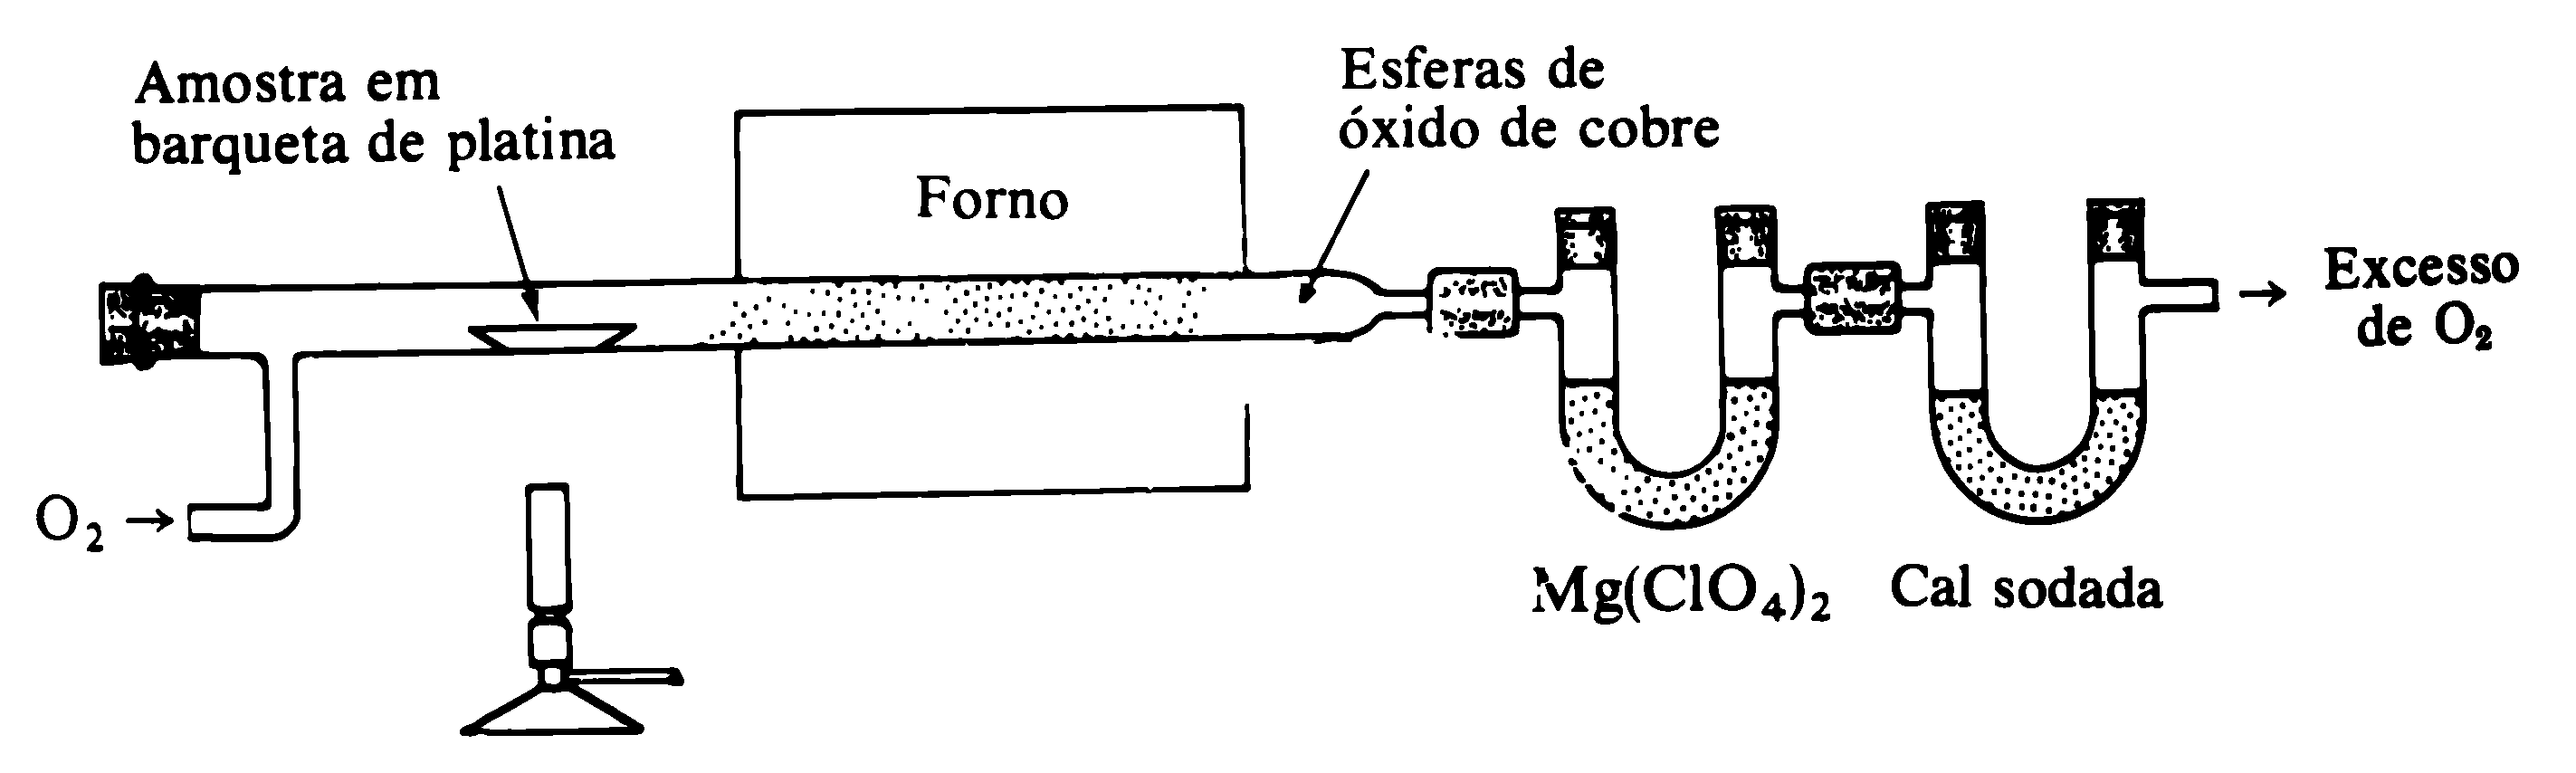
\includegraphics[scale=0.3]{content/images/Figura_2_1.pdf}
    \caption{Representação esquemática da aparelhagem usada para a analise de carbono e hidrogênio.}
    \label{figurar_2_1}
\end{figure}

Conhecendo as quantidades de dióxido de carbono e água produzidas no processo de combustão e a quantidade inicial de matéria orgânica queimada, pode-se calcular a percentagem de carbono e hidrogênio existentes na amostra original. O seguinte exemplo mostra o procedimento adequado. Usando os pesos atômicos H = 1,008, C = 12,01 e O = 16,000, o peso de hidrogênio na amostra é igual ao peso de água produzida vezes a fração de hidrogênio contida na água e o peso de carbono, o peso de dióxido de carbono produzido vezes a fração de carbono contida no dióxido de carbono.

\begin{tightcenter}
    \footnotesize
    g H = g \ch{H2O} $\times$ $\dfrac{2,016}{18,016}$ $\dfrac{\text{g H}}{\text{g \ch{H2O}}}$
    
    \% H = $\dfrac{\text{g H}}{\text{g Amostra}}$ $\times$ 100
    
    g C = g \ch{CO2} $\times$ $\dfrac{12,01}{44,01}$ $\dfrac{\text{g C}}{\text{g \ch{CO2}}}$
    
    \% C = $\dfrac{\text{g C}}{\text{g Amostra}}$ $\times$ 100
\end{tightcenter}

A análise não fornece diretamente a percentagem de oxigênio no composto. Pode-se, entretanto, supor que a percentagem da amostra que não seja carbono ou hidrogênio, e que se sabe não ser outro elemento (de testes preliminares), seja oxigênio, que é, assim, obtido por diferença. 
\end{leftbar}

\par\bigskip
\noindent\emph{No tempo de Liebig, os químicos orgânicos faziam suas próprias análises por combustão e era muito importante, para eles, entender os detalhes experimentais da combustão, pois a precisão obtida na análise dependia dos cuidados tomados durante a experiência. Hoje, o químico orgânico dificilmente faz as análises de que necessita, pois a área é controlada por um grupo de especialistas. Dada a amostra de um composto, eles darão ao químico orgânico a percentagem de cada elemento na amostra. O que é mais importante para o químico médio é que seja capaz de, urna vez conhecidas as percentagens dos elementos presentes, deduzir a fórmula para o composto em estudo. Deve ficar bem claro que a análise determina a percentagem de elementos na amostra. Se o composto não está puro, não serão obtidos bons resultados. Por outro lado, uma boa análise é evidência da pureza do composto.}
\par\bigskip

Como calculamos a fórmula de um composto, uma vez que a composição percentual é fornecida? Como um exemplo, seja a análise por combustão do éter metílico (um gás). Suponhamos que os seguintes valores fossem encontrados:

\begin{tightcenter}
53,24\% de carbono

13,05\% de hidrogênio
\end{tightcenter}

Testes qualitativos mostraram a ausência de outros elementos e, já que a percentagem total não atinge 100\%, a diferença deve ser devida ao oxigênio: 

\begin{tightcenter}
34,71\% de oxigênio 
\end{tightcenter}

Uma amostra de 100 g do composto, por exemplo, conteria 52,4 g de carbono, 13,05 g de hidrogênio e 34,71 g de oxigênio. Usando os números relativos em gramas destes elementos, queremos achar os números relativos em moles. Usando os pesos atômicos já fornecidos teremos em 100 g do composto:

\begin{tightcenter}
52,24/12,01 = 4,36 moles de carbono 

13,05/1,008 = 12,93 moles de hidrogênio 

34,71/16,00 = 2,16 moles de oxigênio 
\end{tightcenter}

Nossa tentativa inicial dá a fórmula C$_{4,36}$H$_{12,93}$O$_{2,16}$. Esta fórmula nos dá as razões corretas dos elementos. É evidente que a molécula contém menos átomos de oxigênio do que de carbono e hidrogênio. Como os átomos ocorrem apenas em números inteiros, então a molécula deve conter pelo menos um átomo de oxigênio, embora possa conter dois, três ou mesmo algum número maior. Se tomarmos os subscritos da fórmula e os dividirmos pelo menor deles (2,16) obteremos as razões corretas entre os elementos, na base da presença de um único átomo de oxigênio. A fórmula que obteremos é C$_{2,02}$H$_{5,98}$O. Existe sempre um erro experimental na análise (menor do que 0,3\%, se a análise for bem feita), e a fórmula que obtivemos, embora não tivesse números inteiros, pode ser tomada como sendo \ch{C2H6O}. Esta fórmula é chamada a \textit{fórmula empírica} do composto. É a fórmula, com a razão correta dos elementos, descrita pelo \textit{conjunto dos menores números inteiros}. A fórmula verdadeira poderia ser um múltiplo da fórmula que obtivemos. Por exemplo \ch{C4H12O2}, que contém exatamente a mesma razão elementar. Poderia ser, também, \ch{C6H18O3}, ou outro qualquer múltiplo da fórmula empírica. Para saber qual destas possibilidades representa a verdadeira \textit{fórmula molecular} do composto é preciso conhecer o peso molecular. Para um gás, o peso molecular pode ser obtido de medidas de pressão, volume e temperatura; para um líquido ou sólido, a partir do abaixamento do ponto de fusão de um solvente apropriado, ou, ainda, de várias outras maneiras. Digamos que para nosso composto, que é um gás, o peso de uma amostra de volume, pressão e temperatura conhecidos indica o peso molecular de 44,5. Para a fórmula empírica \ch{C2H6O} o peso molecular seria 46,1 ou um múltiplo deste número. Como o peso molecular experimental é mais próximo de 46,1 do que de qualquer um de seus múltiplos, podemos garantir que a fórmula molecular do composto é \ch{C2H6O}.

A importância de serem obtidas análises acuradas pode ser medida pelo exemplo seguinte. O ciclo-hexano tem a fórmula molecular \ch{C6H12}, enquanto que o composto chamado ciclo-hexeno, que possui propriedades diferentes, tem fórmula molecular \ch{C6H10}. A percentagem dos dois elementos presentes nestes compostos é, para \ch{C6H12}, de 85,6\% de carbono e 14,4\% de hidrogênio e, para \ch{C6H10}, de 87,7\% de carbono e 12,3\% de hidrogênio. O método analítico desenvolvido por Liebig tornou possível uma precisão de 0,3\% por elemento. Assim, o método de Liebig é capaz de distinguir entre os dois compostos mencionados. 

A desvantagem do método de Liebig, tal como era usado, é que requer uma quantidade que vai de 0,5 a 1,0 g de material para uma análise. O isolamento de um composto orgânico da natureza em forma pura é, frequentemente, muito difícil e muitos dos compostos que têm sido estudados nos últimos anos têm sido obtidos em quantidades muito pequenas. Um processo de microanálise foi introduzido por Pregl, em 1911, utilizando o método básico de Liebig, mas melhorando todos os instrumentos e acessórios envolvidos, especialmente a sensibilidade da balança usada para as pesagens. Pregl foi capaz de desenvolver o método de forma a que a análise fosse possível com 3 a 4 mg do material e recebeu o Prêmio Nobel por este trabalho.

\par\bigskip
\noindent\emph{Embora as fórmulas moleculares sejam, ainda hoje, determinadas pelo método de Pregl, outro método para efetuar esta determinação faz uso de um instrumento chamado espectrômetro de massas. Este aparelho bombardeia moléculas em fase gasosa com um feixe de elétrons. íons positivos, correspondendo à molécula original menos um elétron e aos diversos fragmentos moleculares, são formados e separados de acordo com a sua massa. Das massas destes íons é possível deduzir a fórmula molecular exata. O alto custo dos espectrômetros de massas (US\$30.000,00 a US\$100.000,00) temi evitado que este método seja mais difundido, mas isto ocorrerá certamente no futuro. O espectrômetro de massas será discutido com mais detalhes no Capítulo 32.}
\par\bigskip

\section{A TEORIA ESTRUTURAL DE KEKULÉ}

No campo da química inorgânica, uma vez conhecida a fórmula da substância, frequentemente a fórmula estrutural da molécula pode ser escrita sem problemas. Por exemplo. só existe um composto com a fórmula molecular \ch{Na2SO4}. O mesmo não acontece na química orgânica. Dois compostos, por exemplo, têm a fórmula molecular \ch{C4H10} e 14 compostos têm a fórmula molecular \ch{C5H12O}. Cada um destes 14 compostos têm propriedades físicas diferentes, tais como ponto de fusão e solubilidade e, consequentemente, correspondem a diferentes moléculas. Uma vez que esses compostos têm a mesma fórmula, deve haver algo diferente entre eles, isto é, os átomos devem estar ligados entre si de maneiras diferentes, de modo que a diferentes arranjos corresponderão diferentes compostos. A importância de entender como os átomos se ligam entre si para formar moléculas já era compreendida pelos cientistas nos começos do século XIX, mas os químicos do tempo não tinham como resolver o problema. A solução foi produzida independentemente por Kekulé e Cooper, em 1858. Estes cientistas postularam que o carbono teria a mesma valência 4 em moléculas orgânicas complicadas que têm nas substancias simples tais como tetracloreto de carbono (\ch{CCl4}) e dióxido de carbono (\ch{CO2}). O hidrogênio e o cloro têm valência 1, o oxigênio 2 e o nitrogênio trivalente 3. O carbono poderia ligar-se, então, a quatro átomos de cloro para formar metano (\ch{CH4}) ou a quatro átomos de cloro para formar tetracloreto de carbono. Usando essas valências, poderíamos escrever as fórmulas abaixo para dióxido de carbono, cianeto de hidrogênio (ácido cianídrico), metil-amina e etano:

\begin{tightcenter}
    \chemnameinit{}
    \chemname{\setchemfig{atom sep=2em}\chemfig[][]{Cl-C(-[2]Cl)(-[6]Cl)-Cl}}{\footnotesize{Tetracloreto de carbono}}
    \qquad\qquad\qquad
    \chemnameinit{}
    \chemname{\setchemfig{atom sep=2em}\chemfig[][]{O=C=O}}{\footnotesize{Dióxido de carbono}}
    \qquad\qquad\qquad
    \chemnameinit{}
    \chemname{\setchemfig{atom sep=2em}\chemfig[][]{H-C~N}}{\footnotesize{Cianeto de hidrogênio}}
\end{tightcenter}

\begin{tightcenter}
    \chemnameinit{}
    \chemname{\setchemfig{atom sep=2em}\chemfig[][]{H-C(-[2]H)(-[6]H)-H}}{\footnotesize{Metano}}
    \qquad\qquad\qquad
    \chemnameinit{}
    \chemname{\setchemfig{atom sep=2em}\chemfig[][]{H-C(-[2]H)(-[6]H)-C(-[2]H)(-[6]H)-H}}{\footnotesize{Etano}}
    \qquad\qquad\qquad
    \chemnameinit{}
    \chemname{\setchemfig{atom sep=2em}\chemfig[][]{H-C(-[2]H)(-[6]H)-N(-[2]H)-H}}{\footnotesize{Metil-amina}}
\end{tightcenter}
 
Quando duas moléculas diferentes têm a mesma fórmula molecular são chamadas de \textit{isômeros}. Álcool etílico e éter dimetílico são isômeros com fórmula molecular \ch{C2H6O}: 

\begin{tightcenter}
    \chemnameinit{}
    \chemname{\setchemfig{atom sep=2em}\chemfig[][]{H-C(-[2]H)(-[6]H)-C(-[2]H)(-[6]H)-OH} = \ch{CH3CH2OH}}{\footnotesize{Álcool etílico}}
    \qquad\qquad\qquad
    \chemnameinit{}
    \chemname{\setchemfig{atom sep=2em}\chemfig[][]{H-C(-[2]H)(-[6]H)-O-C(-[2]H)(-[6]H)-H } = \ch{CH3OCH3}}{\footnotesize{Éter dimetílico}}
\end{tightcenter}

Deve ficar bem claro ao leitor que, segundo as regras de valência de Kekulé, estas são as duas únicas maneiras em que estes átomos podem ser arranjados. 

Como dizer experimentalmente a qual estrutura corresponde determinado composto é um problema com o qual nos preocuparemos nos próximos capítulos. 

\section{A LIGAÇÃO COVALENTE}

Kekulé usava uma linha simples para representar a ligação química entre dois átomos, mas não estava clara qual a natureza física desta ligação química. O desenvolvimento do que consideramos, atualmente, uma teoria razoável sobre a natureza das ligações químicas e as estruturas das moléculas orgânicas só foi possível após a descoberta do elétron, em 1897, por J. J. Thompson, e a posterior descrição devida a Lorde Rutherford, em 1911, de um átomo como sendo um sistema formado por pequeno núcleo positivo cercado por elétrons a uma distância relativamente grande. 

Em 1916, Lewis em Berkeley e W. Kossel, em Munique, utilizaram-se do modelo de Rutherford para explicar muitas das propriedades químicas dos átomos e de seus íons. Lewis desenvolveu o modelo, de modo a incluir as ligações covalentes de maneira a permitir a expressão das primeiras idéias sobre a teoria estrutural em termos das partículas fundamentais, núcleo e elétron. A teoria de Lewis é fundamental para o entendimento das estruturas de compostos e das propriedades químicas de moléculas orgânicas em termos clássicos e, graças à sua simplicidade, ainda hoje é largamente utilizada para descrições qualitativas de fenômenos da química orgânica. 

Desde os começos de sua ciência, os químicos orgânicos imaginaram teorias que pudessem explicar suas observações. Uma boa teoria explica todos os fatos nos quais é baseada e pode ser utilizada para a previsão de novos fatos que, por sua vez, podem ser verificados pela experiência. Por causa do desconhecimento, durante o século XIX, da natureza do átomo, as teorias sobre as estruturas e reações de moléculas orgânicas não se desenvolveram com rapidez para ser de valor na predição de novos fatos. Ao contrário, os químicos estavam principalmente preocupados com a explicação de fatos já conhecidos experimentalmente. No entanto, as idéias de Kekulé e de seus contemporâneos eram essencialmente corretas, e os modernos químicos têm a maior admiração pelos cientistas que fizeram o extraordinário trabalho de deduzir as estruturas das moléculas muito antes que os fatos correspondentes aos átomos fossem compreendidos. 

Todavia muitos dos problemas estruturais mais complicados não foram entendidos até cerca de 1930, quando a teoria quantomecânica foi desenvolvida. Não seguiremos, neste capítulo, o desenvolvimento histórico da teoria estrutural por ser um caminho extremamente difícil e trabalhoso, embora de proveito intelectual. Utilizando-nos das idéias essenciais da teoria estrutural, é possível deduzir praticamente todos os fatos relativos as estruturas das moléculas orgânicas nos quais estaremos interessados. Este modo de abordar o problema é vantajoso, no momento, porque liberta o estudante da necessidade de tratar uma quantidade enorme de fatos experimentais e mostra como todos os fatos se tornam evidentes, desde que a teoria seja compreendida. Deve ser enfatizado, entretanto, que, historicamente, tudo se passou de maneira diferente. 

Podem-se reconhecer três tipos de ligação: iônica, metálica e covalente. A \textit{ligação iônica} (\textit{e.g.} \ch{NaCl}) foi muito bem descrita por Lewis e também por Kossel. Na verdade, não se trata de uma ligação, na acepção do termo, mas uma atração eletrostática sem direção preferencial. A \textit{ligação metálica} é característica dos metais em fase sólida e líquida e não nos interessa discuti-la presentemente. Moléculas orgânicas são formadas por átomos em \textit{ligação covalente} e tais ligações formam a base da química orgânica. A teoria de Lewis foi a primeira etapa na compreensão da ligação covalente e, qualitativamente, as idéias em que se baseava estavam essencialmente corretas, já que explicavam a maior parte dos fenômenos. A ligação covalente existe entre pares, de átomos que tendem a completar suas camadas eletrônicas por partilha de elétrons e é, geralmente, mais forte quando um ou ambos os átomos pertencem a um dos grupos centrais da tabela periódica. Um átomo de carbono dificilmente forma ligações iônicas, pois, para tal, seria necessária uma carga +4 ou -4 concentrada em um átomo relativamente pequeno — uma situação altamente desfavorável energeticamente.

\begin{tightcenter}
    C: 1s$^2$2s$^2$2p$^2$ \ch{->} 1s$^2$2s$^0$p$^0$ ou C$^{4-}$: 1s$^2$2s$^2$2p$^6$
\end{tightcenter}

Em vez de perder ou ganhar elétrons de forma definitiva para formar íons, um átomo de carbono tende a partilhar elétrons em ligações covalentes. Muitas moléculas inorgânicas são igualmente formadas por ligações covalentes, como \textit{e.g.}, \ch{N2}, \ch{AsCl3} e \ch{H2O}. 

\par\bigskip
\noindent REVISÃO DAS ESTRUTURAS DE LEWIS. \textit{Será necessário ao leitor recordar o que são estruturas de Lewis, como se representam e o que é} carga formal. \textit{Os próximos parágrafos o ajudarão nisto.} 

\emph{Lewis notou que os sistemas eletrônicos dos gases nobres podem ser considerados como sendo compostos de camadas de elétrons, contendo nas camadas eletrônicas exteriores, respectivamente, 2 elétrons (hélio), 8 elétrons (neônio), 8 elétrons (argônio) e assim por diante. Os gases nobres são muito estáveis e inertes quimicamente. Sistemas eletrônicos semelhantes apresentam, também, relativa estabilidade e inércia química. Temos, assim, F$^-$ com a configuração eletrônica do neônio e K$^+$ com a configuração do argônio. Metano, amoníaco, água e fluoreto de hidrogênio têm, também, 8 elétrons na camada exterior do elemento pesado (desde que contemos os elétrons partilhados) e 2 elétrons na camada eletrônica dos hidrogênios. Todas essas moléculas são eletronicamente análogas aos gases nobres e são substâncias covalentes muito estáveis. Suas estruturas podem ser representadas como se segue:}

\begin{tightcenter}
    \chemnameinit{}
    \chemname{\chemfig[][]{\lewis{0:2:4:6:,C}(-[2,0.4,,,draw=none]H)(-[4,0.4,,,draw=none]H)(-[6,0.4,,,draw=none]H)(-[0,0.4,,,draw=none]H)}}{\footnotesize{Methano}}
    \qquad    
    \chemnameinit{}
    \chemname{\chemfig[][]{\lewis{0:2:4:6:,N}(-[4,0.4,,,draw=none]H)(-[6,0.4,,,draw=none]H)(-[0,0.4,,,draw=none]H)}}{\footnotesize{Amoníaco}}
    \qquad    
    \chemnameinit{}
    \chemname{\chemfig[][]{\lewis{0:2:4:6:,O}(-[4,0.4,,,draw=none]H)(-[6,0.4,,,draw=none]H)}}{\footnotesize{Água}}
    \qquad\qquad\qquad    
    \chemnameinit{}
    \chemname{\chemfig[][]{\lewis{0:2:4:6:,F}(-[4,0.4,,,draw=none]H)}}{\footnotesize{Fluoreto de hidrogênio}}
    \qquad\qquad\qquad    
    \chemnameinit{}
    \chemname{\chemfig[][]{\lewis{0:,He}}}{\footnotesize{Hélio}}
    \qquad    
    \chemnameinit{}
    \chemname{\chemfig[][]{\lewis{0:2:4:6:,Ne}}}{\footnotesize{Neônio}}
\end{tightcenter}

\emph{Para determinar a carga formal de um átomo, contam-se todos os elétrons que, na formula de Lewis, pertencem exclusivamente ao átomo, mais a metade dos elétrons partilhados em ligações covalentes. Se este número é igual ao número de elétrons de valência do átomo livre, a carga formal do átomo na fórmula de Lewis é zero. Se o número de elétrons excede o número de elétrons de valência do átomo livre por 1, 2, 3, ..., então a carga formal do átomo na estrutura de Lewis é -1, —2, —3, .... Se, por outro lado, o numero de elétrons é menor do que o número de elétrons de valência do átomo livre por 1, 2, 3, ..., então a carga formal do átomo na estrutura de Lewis é +1, +2, +3, ....}

\emph{Alguns exemplos do cálculo de cargas formais podem ilustrar melhor o exposto. Na molécula de metano cada átomo tem uma carga formal zero, uma vez que a metade do número de elétrons em ligação covalente é igual ao número de elétrons de valência do átomo de carbono livre (carga formal = 4 - 4 = O), o mesmo acontecendo para os hidrogênios (carga formal = 1 - 1 = O). Pode ser igualmente verificado que todos os átomos em \ch{NH3}, \ch{H2O} e \ch{HF} têm carga formal zero.}

\emph{Examine, agora, as estruturas abaixo:}

\begin{tightcenter}
    \chemnameinit{}
    \chemname{\chemfig[][]{\lewis{0:2:4:6:,\chemabove{N}{\hspace{+5mm}\scriptstyle +}}(-[2,0.4,,,draw=none]H)(-[4,0.4,,,draw=none]H)(-[6,0.4,,,draw=none]H)(-[0,0.4,,,draw=none]H)}}{\footnotesize{Íon amônio}}
    \qquad
    \chemnameinit{}
    \qquad 
    \chemfig[][]{\lewis{0:4:,C}(-[4,0.4,,,draw=none]H)}
\end{tightcenter}


\emph{Note que todos os átomos têm 8 elétrons na camada de valência (exceto os hidrogênios que têm 2). O íon amônio tem 1/2 $\times$ 8 = 4 elétrons que pertencem ao nitrogênio. Como o nitrogênio isolado tem 5 elétrons, há uma carga formal +1 no nitrogênio do íon amônio.}

\emph{Na molécula \ch{HCN}, o H tem uma carga formal zero (1 - 2/2), assim como o carbono (4 - 8/2) e o nitrogênio (5 - 2 - 6/2). No caso do \ch{CN-}, o nitrogênio tem formalmente 5 elétrons e carga formal zero, enquanto o carbono tem 5 elétrons e, portanto, carga formal -1.}

\par\bigskip
O leitor deve lembrar-se de que a descrição exata do átomo de hidrogênio pode ser obtida pela solução da equação de Schrödinger: 

\begin{equation}
    \setlength{\topsep}{.5ex}
    H\psi = E\psi
\end{equation}

\noindent onde existe um conjunto infinito de funções de onda psi ($\psi$) chamadas \textit{orbitais}. Cada orbital é uma função matemática que descreve uma distribuição possível do elétron no espaço. Cada um destes orbitais tem uma energia (\textit{E}) a ele associada. O elétron pode ocupar qualquer um destes orbitais e os átomos adquirem a energia correspondente. 

\par\bigskip
\noindent\emph{O resto desta seção e parte do material subsequente referir-se-á à solução da equação de Schrödinger. A matemática necessária para solucionar a equação é muito complicada e, neste texto, estaremos muito mais interessados em usar os resultados que podem ser obtidos do que nos detalhes de sua obtenção.}
\par\bigskip

A parte complicada da equação é \textbf{H}, o operador Hamiltoniano. (Um operador é um símbolo matemático que nos diz como manipular a quantidade que o segue.) Este operador contém as segundas derivadas de $\psi$ com respeito às coordenadas. Para resolver a equação, deve-se integrá-la. Infelizmente, isto só pode ser feito de maneira exata em alguns casos, tais como o do átomo de hidrogênio. Soluções aproximadas (com muitos algarismos significativos) já foram obtidas para átomos de baixo número atômico e para algumas moléculas pequenas. Mesmo o átomo de hélio já é muito complicado para que se possa obter, com as técnicas de hoje, uma solução exata, mas a energia pode ser calculada por métodos aproximados até 8 algarismos significativos. Não há dúvida nenhuma de que a equação é igual-mente válida para moléculas maiores, mas, para estes casos, mesmo os métodos aproximados de que dispomos são limitados, dada a complexidade matemática do problema. 

O sistema mais simples que contém uma ligação covalente normal (um par de elétrons) é a molécula de hidrogênio (\ch{H2}). Esta molécula vem sendo estudada teoricamente com cuidado. É mais complicada do que o átomo de hélio, embora se pareça muito com ele. Se chamarmos os dois núcleos de hidrogênio da molécula \ch{H2}, H$_A$ e H$_B$, podemos usar o orbital atômicos 1s do hidrogênio para cada um dos átomos ($\psi _A$ e $\psi _B$) e escrever um \textit{orbital molecular} $\psi _A + \psi _B$. No nosso caso, o orbital molecular é formado por uma combinação linear de orbitais atômicos. Do mesmo modo que um orbital atômico nos diz onde o elétron deve ser encontrado no espaço tridimensional ao redor do núcleo, um orbital molecular nos diz onde deve encontrar-se o elétron no espaço tridimensional da molécula. (Lembre-se de que o valor de $\psi ^2$ em qualquer ponto deste espaço é proporcional à densidade eletrônica,, isto é, à probabilidade de encontrar-se o elétron naquele ponto.) A forma do orbital molecular ou a função da probabilidade de encontrar-se um elétron no espaço tridimensional da molécula é, geralmente, muito mais complicada do que a de um orbital atômico. Como acontece com o átomo de hélio, quanto mais refinados os cálculos, melhor a concordância entre os valores experimentais e calculados para as distâncias de ligação e energias. A idéia de que os orbitais moleculares sejam formados por combinações de orbitais atômicos é muito importante. Ela nos permite interpretar a estrutura das moléculas em termos das estruturas dos átomos, os quais conhecemos relativamente bem, graças à analogia que podemos fazer com o caso do átomo de hidrogênio, no qual a equação de Schrödinger pode ser resolvida exatamente. \textit{A matemática da formação de orbitais moleculares é de tal natureza que, em geral, se começamos com n orbitais atômicos e os combinamos, obteremos sempre n orbitais moleculares.} As energias dos n orbitais moleculares serão diferentes das energias dos orbitais atômicos dos quais foram formados. Alguns dos orbitais têm energia mais baixa e são chamados orbitais ligantes, enquanto outros têm energia mais alta e são chamados orbitais antiligantes. Pode acontecer que um, ou mais de um, dos orbitais moleculares tenha a mesma energia do que um dos orbitais atômicos e, neste caso, é chamado orbital não-ligante. Para a molécula de hidrogênio, a solução da equação de Schrödinger dá dois orbitais moleculares ($\psi$ e $\psi ^*$) que são combinações dos orbitais atômicos: 

\begin{equation}
    \setlength{\topsep}{.5ex}
    \psi = \psi _A + \psi _B
    \qquad e \qquad
    \psi ^* = \psi _A - \psi _B
\end{equation}

O primeiro dos orbitais ($\psi$) é um orbital ligante, enquanto o segundo ($\psi ^*$) é antiligante (veja Figura 2.2). Os orbitais moleculares são como os orbitais atômicos, no sentido de que são capazes de suportar no máximo dois elétrons e, assim mesmo, se tiverem spins opostos. É evidente que ambos os elétrons da molécula do hidrogênio ocuparão o orbital ligante (de menor energia) e, nestas circunstâncias, a energia do sistema será mínima quando a separação entre os dois núcleos for de 0,74 \AA ngstrom (\AA). Estes elétrons de ligação estão, portanto, numa situação de maior estabilidade do que estariam, se cada elétron estivesse em um átomo de hidrogênio isolado, e tendem a permanecer nesta situação, mantendo unidos os núcleos e formando uma ligação química. Mais precisamente, eles formam uma ligação com um comprimento de 0,74 \AA \enspace e com força de ligação correspondente à profundidade do poço de potencial no qual estão os elétrons. Por outro lado, elétrons colocados em orbitais antiligantes evitam a região do espaço entre os núcleos, tendendo, deste modo, a mantê-los separados. 

\begin{figure}[H]
    \centering
    \begin{tikzpicture}[help lines/.style={thin,draw=black!50}]
        %\draw[help lines] (0,0) grid (15,12);
        \node (z) at (3,2.2) {\footnotesize{($\psi _A - \psi _B$)}};
        \node (y) at (3,0.6) {\footnotesize{$(\psi _A + \psi _B$)}};
        \node (x) at (4.7,-0.2) {\footnotesize{\textit{d}}};
        \draw [->,>=stealth] (4.85,-0.22) -- ++(0:0.7);
        \node (m) at (-0.2,1.55) {\footnotesize{0}};
        \node [rotate=90] (t) at (-0.5,1.55) {\footnotesize{\textbf{Energia}}};
        \draw [->,>=stealth] (t) -- ++(90:1.5);
        
        % Set horizontal range 
        \pgfmathsetmacro{\nx}{8}
        % Set vertical range 
        \pgfmathsetmacro{\ny}{2.5}
        
        \pgfmathsetmacro{\xmin}{2*(sqrt(\ny+1)-1)/\ny}
        \pgfmathsetmacro{\xmint}{2/sqrt(\ny)}
        \pgfmathsetmacro{\xminb}{4/\ny}
        \pgfmathsetmacro{\xmax}{2*\nx}
        
        \begin{axis}[xmin=0,xmax=\xmax,axis x line*=bottom,axis y line*=left,xtick=\empty,ytick=\empty,extra x ticks={2},extra x tick labels={\footnotesize{0,74 \AA}}]
            \addplot[thick,domain=\xmin:\xmax,samples=100]{1/x^2-1/x+0.05};
            %\addplot[domain=\xminb:\xmax,samples=100]{-1/x};
            \addplot[thick,domain=\xmint:\xmax,samples=100]{1/x^2};
            \addplot[no markers] coordinates {(0,0) (\xmax,0)};
        \end{axis}
    \end{tikzpicture}
    \caption{Energia de dois átomos de hidrogênio em função da distância (\textit{d}) entre os núcleos quando os elétrons ocupam orbitais ligantes é antiligantes.}
    \label{figura_2_2}
\end{figure}

\begin{figure}[H]
    \centering
    \adjustbox{margin=1em,width=\textwidth,set height=4cm,set depth=4cm,frame,center}{Dummy}
    \caption{Orbital de ligação da molécula do hidrogênio.}
    \label{fig2_3}
\end{figure}

Desde o tempo de Kekulé, os químicos orgânicos usam uma linha simples para representar uma ligação covalente e ainda hoje o fazem. Todavia, nossa compreensão do que a linha simples realmente representa alterou-se muito. graças ao nosso melhor conhecimento dos fenômenos que governam a ligação química. Vários outros modos de representação dos orbitais moleculares encontram-se na Figura \ref{fig2_3}. A maneira mais simples de representar os orbitais $1s$ é utilizando-se de círculos. Deve-se, entretanto, ter em mente que cada círculo representa na realidade uma esfera que contém uma boa parte, digamos 90\%, da densidade eletrônica do orbital em seu interior. A Figura ensombrecida representa a probabilidade de distribuição do elétron: quanto mais forte for a sombra, maior será a probabilidade de encontrar-se o elétron naquela posição. Um mapa de contorno de densidade eletrônica frequentemente é útil. A ligação existente na molécula \ch{H2} é uma ligação covalente típica, semelhante àquelas encontradas em moléculas orgânicas. Em uma molécula complicada é, geral-mente, uma boa aproximação da realidade considerarem-se os átomos ligados aos pares por ligações covalentes. 

Uma ligação covalente entre quaisquer dois átomos é descrita por uma função de onda que tem uma certa semelhança com a que usamos para a molécula de hidrogênio. Para uma molécula como \ch{HF}, a função de onda para o orbital ligante é tal que existe maior densidade eletrônica no átomo eletronegativo (flúor), como aliás seria de se esperar. A função de onda de ligação para \ch{HF} é $\psi = \psi$H$_{1s} + \lambda\psi$F$_{2p}$, onde lambda ($\lambda$) > 1, correspondendo a uma densidade eletrônica maior na parte F$_{2p}$ do orbital de ligação do que na parte H$_{1s}$. 

Por outro lado, o elétron no orbital antiligante gasta a maior parte de seu tempo perto do elemento eletropositivo. As densidades eletrônicas correspondentes aos orbitais ligante e antiligante da molécula do fluoreto de hidrogênio estão na Figura \ref{fig2_4}. (Os átomos de flúor têm muitos elétrons não-ligantes que não aparecem na Figura. Observe que o átomo de flúor usa um orbital $2p$ para formar a ligação.) Se os elétrons estão no orbital de ligação, tendem a concentrar-se entre os núcleos. O orbital de antiligação tem um nodo (superfície de densidade eletrônica zero) e os elétrons tendem a evitar esta região. 

\par\bigskip
\noindent\emph{O leitor pode muito bem perguntar: mas como o elétron é capaz de atravessar o nodo? A resposta mais direta é que os nodos são preditos na base de matemática não-relativística e os livros-texto geralmente esquecem-se de mencionar que, quando os efeitos da relatividade são levados em consideração, a superfície de densidade eletrônica "zero" tem uma densidade eletrônica finita (embora muito pequena). O nodo é, portanto, na realidade só uma aproximação e o elétron pode cruzá-lo sem problemas.}
\par\bigskip

O estado de mais baixa energia para a molécula é geralmente aquele que nos interessa mais e é chamado \textit{estado fundamental}. Se dermos energia à molécula (da maneira correta), é possível excitar-se um elétron de um orbital ligante a um orbital antiligante. Esta absorção de energia ocorre apenas em determinados comprimentos de onda (energias) que dependem das diferenças de energia entre o orbital ocupado pelo elétron no estado fundamental e nos diversos estados excitados. As excitações eletrônicas que ocorrem corresponderão ao espectro de absorção da molécula. Um \textit{espectro de absorção} é medido pela diferença de quantidade de radiação incidente em uma substância e a quantidade capaz de atravessá-la. Esta diferença é usada para excitar os átomos ou moléculas a estados de mais alta energia. Frequentemente o espectro de absorção de uma substância permite inferir-se muitas informações relevantes sobre a estrutura molecular; por isto voltaremos ao assunto em capítulos subsequentes. 

\begin{figure}[H]
    \centering
    \adjustbox{margin=1em,width=\textwidth,set height=4cm,set depth=4cm,frame,center}{Dummy}
    \caption{Orbitais ligantes e antiligantes do fluoreto do hidrogênio.}
    \label{fig2_4}
\end{figure}

A cor amarela que aparece em uma chama toda vez que nela colocamos um pouco de sódio é um exemplo familiar de \textit{espectro de emissão}. O sódio adquire energia térmica da chama e os seus elétrons são excitados a orbitais de mais alta energia. Quando os elétrons voltam aos níveis de mais baixa energia, luz de diversos comprimentos de onda é emitida, inclusive na região do visível, e, assim, podemos ver a cor amarela característica. O espectro de emissão é medido pela radiação fornecida quando os elétrons voltam dos estados excitados ao fundamental.

\section{ESTRUTURA DO METANO}

o metano é o constituinte principal do gás natural que usamos como combustível. Algumas vezes é chamado \textit{gás dos pântanos} porque é o produto da decomposição de vegetais em condições anaeróbicas. O metano tem fórmula \ch{CH4}, e é o \textit{hidrocarboneto} (molécula contendo apenas carbono e hidrogênio) mais simples. No século passado ficou estabelecido que esta molécula tem a forma de um tetraedro regular (Figura \ref{figura_2_5}) com hidrogênios nos quatro vértices e carbono no centro, sendo os ângulos \ch{HCH} de 109,5$\degree$. A prova desta estrutura residia no fato, que pode ser mostrado experimentalmente: os quatro hidrogênios são equivalentes. Assim, existe apenas um cloreto de metileno, \ch{CH_2Cl_2}. Uma vez que os quatro vértices de um tetraedro regular são equivalentes, não faz diferença qual grupo de dois hidrogênios é substituído por cloro, porque a mesma estrutura resultará sempre. Observe que, se a estrutura da molécula fosse a de um quadrado em um plano, por exemplo, os átomos de cloro poderiam estar em vértices adjacentes, ou não, e haveria assim dois compostos com estruturas diferentes e com a fórmula \ch{CH_2Cl_2} (Figura \ref{figura_2_6}).

\begin{figure}[H]
    \centering
    \begin{tikzpicture}[help lines/.style={thin,draw=black!50}] 
        % \draw[help lines] (0,0) grid (15,12);
        \path (0,0) node (m) {C} (2,0) node (x) {H};
        \node (z) at ($ (m) + (100:2) $) {H};
        \node (y) at ($ (m) + (310:2) $) {H};
        \node (w) at ($ (m) + (200:3) $) {H};
        \draw[thick] (m) -- (z);
        \draw[thick] (m) -- (x);
        \draw[thick] (m) -- (y);
        \draw[thick] (m) -- (w);
        \draw[dashed] (x) -- (y) -- (z) -- (x);
        \draw[dashed] (z) -- (w) -- (y) -- (z);
        \draw[dashed] (w) -- (x);
    \end{tikzpicture}
    \caption{Estrutura de tetraedro regular do metano (as linhas interrompidas são imaginarias e são incluídas apenas para facilitar a visualização do tetraedro.}
    \label{figura_2_5}
\end{figure}

\begin{figure}[H]
    \centering
    \begin{tikzpicture}[help lines/.style={thin,draw=black!50}] 
        % \draw[help lines] (0,0) grid (15,12);
        \path (0,0) node (m) {C};
        \node (z) at ($ (m) + (45:2) $) {H};
        \node (x) at ($ (m) + (155:3) $) {H};
        \node (w) at ($ (m) + (225:2) $) {Cl};
        \node (y) at ($ (m) + (334:3) $) {Cl};
        \draw[thick] (m) -- (z);
        \draw[thick] (m) -- (x);
        \draw[thick] (m) -- (y);
        \draw[thick] (m) -- (w);
        \draw[dashed] (z) -- (x) -- (w) -- (y) -- (z);
        % isômero
        \path (7,0) node (m2) {C};
        \node (z2) at ($ (m2) + (45:2) $) {H};
        \node (x2) at ($ (m2) + (155:3) $) {Cl};
        \node (w2) at ($ (m2) + (225:2) $) {H};
        \node (y2) at ($ (m2) + (334:3) $) {Cl};
        \draw[thick] (m2) -- (z2);
        \draw[thick] (m2) -- (x2);
        \draw[thick] (m2) -- (y2);
        \draw[thick] (m2) -- (w2);
        \draw[dashed] (z2) -- (x2) -- (w2) -- (y2) -- (z2);
    \end{tikzpicture}
    \caption{Isômeros que seriam possíveis se o cloreto de metileno fosse um quadrado coplanar.}
    \label{figura_2_6}
\end{figure}

Estudos realizados com muitos metanos substituídos mostram, invariavelmente, que o número total de isômeros é coerente com uma estrutura de tetraedro regular para o metano, eliminando assim todas as demais geometrias possíveis. O carbono tetraédrico foi proposto independentemente por van't Hoff e Le Bel, em 1874, na base de fatos experimentais que discutiremos no Capítulo 3. Esta estrutura é confirmada por muitos tipos diferentes de experiencias físicas e químicas. O porquê de o metano possuir esta estrutura, e não outras aparentemente plausíveis, só foi compreendido com o desenvolvimento da teoria quanto-mecânica, sendo até então aceita como um fato experimental.

Com o desenvolvimento da teoria quanto-mecânica, nos anos 20 e 30, a estrutura do metano pôde ser estudada do ponto de vista teórico. Os átomos de hidrogênio ligados ao carbono utilizam seus orbitais $1s$ para formar a ligação, como no \ch{H2} ou em \ch{HF}. Em seu estado fundamental, um átomo de carbono tem dois elétrons desemparelhados (Figura \ref{figura_2_7}). Dever-se-ia esperar que, em vez de formar \ch{CH4}, o carbono se ligasse a apenas dois hidrogênios, formando \ch{CH2} e deixando um orbital $2p$ vazio. \ch{CH2} é uma espécie química conhecida, chamada carbeno, e é muito reativa, tendo um tempo de vida muito curto. 

A resposta a esta questão foi rapidamente encontrada. Pela adição de 96 quilocalorias por mol (kcal mol$^{-1}$) de energia aos átomos de carbono, um dos elétrons $2s$ pode ser excitado ao orbital $2p$ vazio, dando a configuração mostrada na Figura \ref{figura_2_8}. Agora o átomo de carbono tem quatro elétrons disponíveis para a formação de ligações e, uma vez formadas as ligações covalentes, a configuração semelhante à do gás nobre é obtida (se contarmos como pertencendo à camada exterior, ou de valência, todos os elétrons que nela estão, seja pertencendo apenas ao átomo em questão, seja partilhados com outros átomos). A formação da ligação covalente resulta no abaixamento da energia do par de elétrons envolvidos, como vimos para o caso da reação \ch{2 H -> H2} (Seção 2.4). Na reação \ch{CH2 + 2 H -> CH4} formam-se duas ligações \ch{C—H}, o que resulta em um decréscimo de energia da ordem de 174 kcal mol$^{-1}$. Este decréscimo supera de muito o aumento de 96 kcal mol$^{-1}$ que foi necessário para levar o átomo do estado fundamental ao estado excitado que mostramos na Figura \ref{figura_2_8}, e explica porque o carbono tende a ser tetravalente. Monóxido de carbono (\ch{C=O}) é o único composto divalente de carbono estável. 

\begin{figure}[H]
    \centering
    \begin{tikzpicture}[help lines/.style={thin,draw=black!50}] 
        %\draw[help lines] (0,0) grid (15,12);
        \foreach \x in {10,...,14} 
            \draw[thick] (\x,9) circle (0.4);
        \foreach \x in {6,...,8} 
            \draw[thick] (\x,8) circle (0.4);
        \draw[thick] (4,7) circle (0.4);
        \foreach \x in {6,...,8}
            \draw[thick] (\x,5) circle (0.4);
        \node at (6,5) {$\uparrow$};
        \node at (7,5) {$\uparrow$};
        \draw[thick] (4,4) circle (0.4);
        \node at (4,4) {$\uparrow \downarrow$};
        \draw[thick] (4,2) circle (0.4);
        \node at (4,2) {$\uparrow \downarrow$};
        \draw[line width=1.5pt,decoration={brace},decorate] (2.5,6.5) -- node[left=5pt] {$n=3$} (2.5,9.5);
        \node at (3,9) {$3d$};
        \node at (3,8) {$3p$};
        \node at (3,7) {$3s$};
        \draw[line width=1.5pt,decoration={brace},decorate] (2.5,3.5) -- node[left=5pt] {$n=2$} (2.5,5.5);
        \node at (3,5) {$2p$};
        \node at (3,4) {$2s$};
        \node at (3,2) {$1s$};
        \node at (1.8,2) {$n=1$};
        \node at (1.8,1) {$l=$};
        \node at (4,1) {$0$};
        \node at (7,1) {$1$};
        \node at (12,1) {$2$};
        \node at (1.8,0) {$m=$};
        \node at (4,0) {$0$};
        \node at (6,0) {$+1$};
        \node at (7,0) {$0$};
        \node at (8,0) {$-1$};
        \node at (10,0) {$+2$};
        \node at (11,0) {$+1$};
        \node at (12,0) {$0$};
        \node at (13,0) {$-1$};
        \node at (14,0) {$-2$};
    \end{tikzpicture}
    \caption{Estado fundamental eletrônico do carbono.}
    \label{figura_2_7}
\end{figure}

\begin{figure}[H]
    \centering
    \begin{tikzpicture}[help lines/.style={thin,draw=black!50}] 
        %\draw[help lines] (0,0) grid (15,12);
        \foreach \x in {6,...,8} {
            \draw[thick] (\x,5) circle (0.4);
            \node at (\x,5) {$\uparrow$};
        }
        \draw[thick] (4,4) circle (0.4);
        \node at (4,4) {$\uparrow$};
        \draw[thick] (4,2) circle (0.4);
        \node at (4,2) {$\uparrow \downarrow$};
        \node at (3,5) {$2p$};
        \node at (3,4) {$2s$};
        \node at (3,2) {$1s$};
    \end{tikzpicture}
    \caption{Estado eletrônico do carbono que se obtém pela excitação de um elétron $2s$ ao orbital vazio $2p$.}
    \label{figura_2_8}
\end{figure}

 Embora não seja difícil perceber-se porque o carbono tende a ser tetravalente, é menos óbvio porque o carbono tende a formar compostos que são tetraedros regulares. Os quatro orbitais de valência da Figura \ref{figura_2_8} são três orbitais $p$, dispostos perpendicularmente uns aos outros, e um orbital $s$, esférico, e, portanto, sem direção definida. Uma ligação química é sempre mais forte quando os núcleos estão na linha de maior densidade eletrônica, de modo que esperaríamos, neste caso, que o átomo de carbono no metano estivesse no vértice de um cubo e três dos hidrogênios estivessem nos vértices a ele adjacentes, correspondendo às direções dos três orbitais $p$. Como o orbital $s$ é esférico, o quarto hidrogênio poderia estar em qualquer direção, como indicado na Figura \ref{figura_2_9}. Isto significaria que três dos ângulos seriam de 90$\degree$ e os demais não poderiam ser especificados. Esta estrutura não pode ser correta porque os quatro hidrogênios, como já vimos, têm de ser equivalentes. 

\begin{figure}[H]
    \centering
    \begin{tikzpicture}[help lines/.style={thin,draw=black!50}] 
        % \draw[help lines] (0,0) grid (15,12);
        \path (0,0) node (x) {H} (0,2) node (m) {C};
        \node (z) at ($ (m) + (20:2) $) {H};
        \node (y) at ($ (m) + (-3:2) $) {H};
        \draw[thick] (x) -- (m) -- (z);
        \draw[thick] (m) -- (y);
        % \node (b) at ($ (x) + (-3:2) $) {};
        \draw[dashed] (x) -- ($ (x) + (-3:2) $) -- (y) -- ($ (y) + (20:2) $) -- ++(-90:2) -- ++(200:2);
        \draw[dashed] (x) -- ($ (x) + (20:2) $) -- ++(-3:2);
        \draw[dashed] (z) -- ++(-90:2);
        \draw[dashed] (z) -- ++(-3:2);
        \draw[] (m) -- ++(90:2);
        \draw[] (m) -- ++(177:2);
        \draw[] (m) -- ++(200:2);
        \draw (-1,2.2) .. controls (-0.9,2.3) .. (-0.8,2.2) .. controls (-0.7,2.3) .. (-0.6,2.2);
        \node (H) at (-1.3,2.3) {H};
    \end{tikzpicture}
    \caption{Estrutura que esperaríamos para o metano se os orbitais de ligação não fossem hibridados.}
    \label{figura_2_9}
\end{figure}

A dificuldade aqui é teórica, uma vez que a evidência experimental é muito grande. O erro deve vir do fato de que estamos formando a ligação \ch{C—H} incorretamente. Os orbitais ($s$ e $p$) que usamos para descrever a molécula não estão corretos. Em outras palavras, o átomo de carbono deve ter sua descrição orbital alterada quando a ligação é feita. O sistema descrito no parágrafo precedente é uma solução aproximada satisfatória da equação Schrõdinger para a camada $n = 2$, mas podemos escrever combinações lineares dos quatro orbitais que são igualmente soluções da equação de Schrõdinger. (Os novos orbitais, obtidos dessas combinações lineares, são chamados de \textit{orbitais híbridos}.) Como construir \textit{orbitais híbridos} que satisfaçam as necessidades de geometria do tetraedro regular? A principal exigência é que os quatro orbitais devem ser equivalentes (de modo a formar quatro ligações \ch{C—H} equivalentes) e, portanto, a combinação linear adequada deve incluir os quatro orbitais de valência da Figura \ref{figura_2_8}. É matematicamente viável fazê-lo e os quatro novos orbitais terão caráter $\dfrac{1}{4} s$ e $\dfrac{3}{4}p$. Os quatro orbitais equivalentes contêm, portanto, três vezes mais caráter $p$ do que $s$ e são chamados orbitais $sp^3$.
\par\bigskip

\begin{leftbar}[cut=false]
\footnotesize

\noindent MATÉRIA OPCIONAL

\noindent \textit{Energética da hibridação}. Como uma ilustração específica, considere o átomo de neônio. A camada $n = 2$ está completa e a nuvem de elétrons total é esférica. (A densidade eletrônica total que resulta da existência de dois elétrons em cada orbital $2p$ é esférica, embora isto não seja aparente da inspeção das formas dos orbitais $p$.) Dois elétrons estão no orbital $2s$, com energia $E_8$ e seis elétrons estão nos orbitais $2p$, com energia $E_p$. A energia eletrônica total é, portanto $2E_8 + 6E_p$.

Se considerarmos quatro orbitais $sp^3$, cada qual com dois elétrons, a energia total é 8 elétrons $\times$ $(\dfrac{1}{4}E_8 + \dfrac{3}{4}E_p) = 2E_8 + 6E_p$, como acima, e os oito elétrons descrevem a mesma distribuição esférica. Assim, a descrição da camada externa do átomo de neônio pode ser feita igualmente em termos de um orbital $s$ e três orbitais $p$, ou em termos de quatro orbitais $sp^3$. Seria a mesma coisa que dizer que 12 é 3 $\times$ 4 ou 2 $\times$ 6. Ambas são corretas mas uma delas pode ser de uso mais conveniente. 

A hibridação dos orbitais não afeta a energia, distribuição eletrônica ou qualquer propriedade do estado fundamental do neônio, de modo que podemos utilizar ou não, a nossa escolha, orbitais híbridos. (Isto não é verdadeiro para estados excitados. Por quê?) 

Em um átomo de flúor, a distribuição eletrônica e a energia total dependem da hibridação e isto pode ser verificado usando-se sete elétrons e fazendo um cálculo semelhante ao que fizemos para o neônio. 
\end{leftbar}
\par\bigskip

Se examinarmos um mapa de contorno da densidade eletrônica de um orbital $sp^3$ veremos que apresenta dois lobos, como um orbital $p$, porém com tamanhos diferentes (Figura \ref{fig2_10}). Sabemos que para que se forme uma ligação forte é preciso que os elétrons de ligaçao possam permanecer entre os núcleos que se ligam. Um orbital $sp^3$, devido à sua forma, tem densidade eletrônica maior em uma direção especifica do que um orbital $s$ ou um orbital $p$ e, assim, devemos esperar que um orbital $sp^3$ possa formar uma ligação consideravelmente mais forte do que os orbitais $s$ ou $p$. Verifica-se, experimentalmente, que a força de uma ligação \ch{C—H} usando um híbrido $sp^3$ é de 103 kcal mol$^{-1}$, enquanto que com orbitais $s$ e $p$ e, respectivamente, de 60 e 80 kcal mol$^{-1}$. 

\begin{figure}[H]
    \centering
    \adjustbox{margin=1em,width=\textwidth,set height=4cm,set depth=4cm,frame,center}{Dummy}
    \caption{Mapa de contorno da densidade eletrônica do orbital $sp^3$.}
    \label{fig2_10}
\end{figure}

Mas toda essa discussão não teria sentido se não fosse pelo fato de que os quatro orbitais $sp^3$ guardam necessariamente entre si os ângulos de 109,5$\degree$, isto é, os ângulos internos do tetraedro regular. 

\begin{figure}[H]
    \centering
    \adjustbox{margin=1em,width=\textwidth,set height=4cm,set depth=4cm,frame,center}{Dummy}
    \caption{Densidade eletrônica em torno de um átomo de carbono com hibridação sp3. Mostramos apenas o maior lobo de cada orbital. Note que a densidade eletrônica total é esférica..}
    \label{fig2_11}
\end{figure}

Os orbitais híbridos $sp^3$ fornecem a melhor descrição do átomo de carbono no metano, porque o átomo de carbono (antes de formar a ligação) tem a mesma energia, hibridado ou não (Figura \ref{fig2_12}), mas a configuração hibridada permite formar ligações mais fortes. Há para a molécula de metano uma vantagem adicional na geometria tetraédrica. Tal arranjo permite o afastamento máximo dos núcleos de hidrogênio para uma dada distância \ch{C-H} e, uma vez que estes núcleos são carregados positivamente, quanto mais afastados os núcleos menor a energia do sistema.

\begin{figure}[H]
    \centering
    \adjustbox{margin=1em,width=\textwidth,set height=4cm,set depth=4cm,frame,center}{Dummy}
    \caption{Descrição eletrônica do carbono tetracovalente.}
    \label{fig2_12}
\end{figure}

Sumariando, o metano é tetraédrico e sua estrutura pode ser considerada como resultando da hibridação de quatro orbitais atômicos ($2s$, $2p_x$, $2p_y$ e $2p-z$), cada um contendo um elétron de valência, a quatro orbitais $sp^3$ equivalentes, os quais permitem a formação de ligações mais fortes e nas direções adequadas para minimizar as repulsões dos núcleos de hidrogênio. Assim, é possível descrever-se matematicamente as ligações da molécula de metano e entender-se o porquê de sua geometria. Melhor ainda, pode-se usar o conceito de orbitais híbridos para se entender moléculas mais complicadas (Seção 4.3). 

\par\bigskip
\noindent SOLUÇÃO DA EQUAÇÃO DE SCHRÖDINGER. \emph{Embora não seja possível a resolução da equação de Schrödinger, de maneira analítica, para moléculas contendo alguns átomos, é, em princípio, possível obter-se uma solução no grau de precisão desejado. Há mais ou menos 30 anos que sabemos como fazê-lo. Executar os cálculos complexos que são necessários é que é o problema. A solução tem de ser obtida usando-se métodos aproximados. Acontece que podemos expressar as propriedades de um átomo em termos de uma série infinita de orbitais e, para moléculas, combinações destas séries infinitas. Na prática reduzimos as séries a um número finito de termos maior ou menor, dependendo da precisão desejada na solução. Na resolução da equação de Schrödinger para uma molécula, é preciso multiplicar entre si muitas destas séries reduzidas, onde cada termo da multiplicação é uma integral de difícil avaliação. É evidente que a matemática envolvida torna o trabalho complicado. Após 1950, entretanto, grande progresso pôde ser feito nestes cálculos, graças ao desenvolvimento de computadores eletrônicos. O computador IBM 360/50, um típico computador de médio porte, de uso largamente difundido, pode executar 150.000 adições ou subtrações com sete algarismos significativos ou 50.000 multiplicações ou, ainda, 5.000 operações mais complexas (potências, raízes, funções trigonométricas) por segundo, com perfeição. Um problema de mecânica quântica pode necessitar de uma hora do tempo do computador e, sem qualquer dúvida, está fora da capacidade de um indivíduo que possua apenas uma régua de cálculo. A solução de problemas que seriam impossíveis em 1950 tornaram-se trabalho rotineiro. Por outro lado, soluções mais exatas para problemas comuns de moléculas poliatômicas (e para enfrentar o problema da reação química) exigirão computadores muito mais rápidos do que o IBM 360/50 (tão distantes em desempenho do IBM 360/50 do que este para as réguas de cálculo). De modo que, por enquanto, a teoria quântica é muito útil para dar respostas aproximadas aos mais diversos problemas da química, porém, exceto para moléculas pequenas, determinações precisas terão de ser feitas experimentalmente.}
\chapter{Os Alcanos}
\section{ESTRUTURA E NOMENCLATURA}
Existe um grande número de hidrocarbonetos com a fórmula \ch{C_{n}H_{2n+2}}. Estes compostos são chamados \textit{alcanos} ou \textit{parafinas}, e metano, \ch{CH4} (Seção 2.5), é o mais simples deles. Pelo aumento de \emph{n} obteremos as fórmulas de uma família de compostos, uma \textit{série homóloga}. Os quatro primeiros termos da série são:

\begin{tightcenter}
    \chemnameinit{}
    \chemname{\setchemfig{atom sep=2em}\chemfig[][]{H-C(-[2]H)(-[6]H)-H}}{\footnotesize Metano}
    \qquad
    \chemname{\setchemfig{atom sep=2em}\chemfig[][]{H-C(-[2]H)(-[6]H)-C(-[2]H)(-[6]H)-H}}{\footnotesize Etano}
    \qquad
    \chemname{\setchemfig{atom sep=2em}\chemfig[][]{H-C(-[2]H)(-[6]H)-C(-[2]H)(-[6]H)-C(-[2]H)(-[6]H)-H}}{\footnotesize Propano}
    \qquad
    \chemname{\setchemfig{atom sep=2em}\chemfig[][]{H-C(-[2]H)(-[6]H)-C(-[2]H)(-[6]H)-C(-[2]H)(-[6]H)-C(-[2]H)(-[6]H)-H}}{\footnotesize Butano}
    \chemnameinit{}
\end{tightcenter}

\noindent Os compostos acima são todos gasosos à temperatura ambiente, e os dois últimos, liquefeitos e colocados em cilindros, são muito usados como combustível. Os homólogos de maior peso molecular - pentano, hexano, octano, nonano, etc. - são líquidos (Tabela \ref{tab3_1}).

\begin{table}[H]
\centering
\caption{Os hidrocarbonetos normais.}
\label{tab3_1}
\begin{tabular}{cccP{4cm}cc}
\toprule
N.$\degree$ de carbonos & Fórmula & Nome & Número total de isômeros possíveis & P.E. ($\degree$C) & P.F. ($\degree$C) \\
\midrule
1 & \ch{CH4} & Metano & 1 & -162 & -183 \\ 
2 & \ch{C2H6} & Etano & 1 & -89 & -172 \\
3 & \ch{C3H8} & Propano & 1 & -42 & -187 \\
4 & \ch{C4H10} & Butano & 2 & 0 & -138 \\
5 & \ch{C5H12} & Pentano & 3 & 36 & -130 \\
6 & \ch{C6H14} & Hexano & 5 & 69 & -95 \\ 
7 & \ch{C7H16} & Heptano & 9 & 98 & -91 \\
8 & \ch{C8H18} & Octano & 18 & 126 & -57 \\
9 & \ch{C9H20} & Nonano & 35 & 151 & -54 \\
10 & \ch{C10H22} & Decano & 75 & 174 & -30 \\ 
11 & \ch{C11H24} & Undecano & - & 196 & -26 \\ 
12 & \ch{C12H26} & Dodecano & - & 216 & -10 \\
20 & \ch{C20H42} & Eicosano & 366.319 & 34 & +36 \\
30 & \ch{C30H62} & Tricontano & $4,11 \times 10^9$ & 446 & +66 \\
\bottomrule
\end{tabular}
\end{table}

\par\bigskip
\noindent\emph{NOMENCLATURA TRIVIAL. A nomenclatura de moléculas orgânicas simples não é completamente sistemática porque os compostos já eram conhecidos e tinham seus nomes próprios antes que suas estruturas fossem conhecidas. Por exemplo, o nome butano veio de um composto a ele relacionado (ácido butírico) que foi isolado pela primeira vez de manteiga rançosa. Os homólogos superiores têm uma nomenclatura mais sistemática, baseada em números gregos. Esses compostos e alguns outros são algumas vezes chamados de hidrocarbonetos alifáticos (do grego aleifar, gordura).}
\par\bigskip

Homólogos de cadeia linear contendo 18 ou mais carbono são sólidos graxos de baixo ponto de fusão, e sua mistura, comercialmente conhecida por graxa de parafina, já foi muito usada para selar garrafas de geléia, mas agora é mais usada como moderador em reatores nucleares. 

As ligações em todos os alcanos são fundamentalmente as mesmas que em metano. Os átomos são ligados por pares de elétrons em orbitais híbridos sp3 dos átomos de carbono e orbitais 1s dos átomos de hidrogênio. Cada carbono tem seus substituintes (átomos ou grupos de átomos a ele ligados) dispostos em um arranjo tetraédrico.

Frequentemente é difícil visualizar-se a estrutura tridimensional de uma molécula. Torna-se então muito útil ter 'modelos moleculares' que ajudem a compreender as estruturas. Existem três tipos principais de modelos, mostrado na Figura \ref{fig3_1}, que são uma aproximação da estrutura  e que tentam dar uma idéia do tamanho físico dos vários átomos. Embora nenhum dos tipos de modelos seja perfeitamente exato, eles têm alguma utilidade, dependendo da propriedade molecular que estejamos examinado. O leitor deverá familiarizar-se como cada tipo de modelo. Nós usaremos os diferentes tipos neste texto, dependendo das necessidades de cada caso. 

\begin{figure}[H]
    \centering
    \adjustbox{margin=1em,width=\textwidth,set height=4cm,set depth=4cm,frame,center}{Dummy}
    \caption{Os vários modelos moleculares representado o etano.}
    \label{fig3_1}
\end{figure}

Não há, em principio, limites para o numero de átomos de carbono que podem ser ligados em uma cadeia de hidrocarboneto. Nos conhecemos atualmente hidrocarbonetos lineares de mais de coem átomos de carbono. Uma das razoes para a existência de tantos compostos orgânicos é que não há verdadeiramente um limite para o tamanho das moléculas que podem ser formadas. Porém, a razão principal para a existência de tantos tipo diferentes de compostos orgânicos é o fenômeno conhecido como isomeria. Você deve lembrar-se que dois compostos diferentes são chamados isômeros se tiverem a mesma formula molecular. Embora propano e os homólogos inferiores não tenham isômeros, existem dois compostos com a formula molecular \ch{C4H10} três com a formula \ch{C5H12} e cinco com a formula \ch{C6H14}. O numero de isômeros aumenta enormemente com o aumento do número de carbonos (Tabela \ref{tab3_1}).

Se escrevemos propano, \ch{C3H8} com valências 4 para o carbono e 1 para o hidrogênio, só uma estrutura é possível. As duas formulas:

\begin{tightcenter}
    \setchemfig{atom sep=2em}\chemfig[][]{CH_3-C(-[2]H)(-[6]H)-CH_3}
    \qquad e \qquad
    \setchemfig{atom sep=2em}\chemfig[][]{H-C(-[2]CH_3)(-[6]CH_3)-H}
\end{tightcenter}

\noindent correspondem à mesma molécula vista de suas posições diferentes e representam a mesma estrutura. A fórmula:

\begin{tightcenter}
    \setchemfig{atom sep=2em}\chemfig[][]{CH_3-C(-[2]H)(-[6]CH_3)-H}
\end{tightcenter}

\noindent é também equivalente às duas outras, embora isto não seja evidente na reapresentação bidimensional, porque os quatro lados do tetraedro regular são equivalentes. Na Figura \ref{fig3_2} mostramos três vista diferentes de um modelo do propano, correspondendo às orientações das três formulas precedentes.

\begin{figure}[H]
    \centering
    \adjustbox{margin=1em,width=\textwidth,set height=4cm,set depth=4cm,frame,center}{Dummy}
    \caption{Três vistas de um modelo do propano \ch{C3H8}.}
    \label{fig3_2}
\end{figure}

À fórmula \ch{C4H10} correspondem duas estruturas moleculares que podem ser escritas:

\begin{tightcenter}
    \chemname{\setchemfig{atom sep=2em}\chemfig[][]{H-C(-[2]H)(-[6]H)-C(-[2]H)(-[6]H)-C(-[2]H)(-[6]H)-C(-[2]H)(-[6]H)-H}}{\footnotesize\emph{n}-butano}
    \qquad\qquad
    \chemname{\setchemfig{atom sep=2em}\chemfig[][]{H-C(-[2]H)(-[6]H)-C(-[2]H)(-[6,1.6]C(-[4]H)(-[6]H)-H)-C(-[10]H)(-[6]H)-C(-[2]H)(-[6]H)-H}}{\footnotesize Isobutano}
    \chemnameinit{}
\end{tightcenter}

\noindent Estas estruturas são diferentes, como pode ser visto na Figura \ref{fig3_3}. Um dos isômeros, isobutano, tem um carbono ligado a três outros carbonos, o que não acontece com o outro isômero, \emph{n}-butano.

\begin{figure}[H]
    \centering
    \adjustbox{margin=1em,width=\textwidth,set height=4cm,set depth=4cm,frame,center}{Dummy}
    \caption{À formula \ch{C4H10} correspondem o $n$-butano (à esquerda) e o isobutano (`a direita).}
    \label{fig3_3}
\end{figure}

Um composto que tem seus átomos de carbono colocados em uma cadeia linear é sempre chamado normal (\emph{n}-). Quando há uma substituição no segundo carbono, o composto é chamado \emph{iso}. Existem três alcanos com cinco carbonos: pentano normal (\emph{n}-pentano), isopentano e neopentano.

\begin{tightcenter}
    \chemname{\setchemfig{atom sep=2em}\chemfig[][]{CH_3-CH_2-CH_2-CH_2-CH_3}}{\footnotesize\emph{n}-pentano}\qquad
    \chemname{\setchemfig{atom sep=2em}\chemfig[][]{CH_3-CH(-[6]CH_3)-CH_2-CH_3}}{\footnotesize isopentano}\qquad
    \chemname{\setchemfig{atom sep=2em}\chemfig[][]{CH_3-C(-[2]CH_3)(-[6]CH_3)-CH_3}}{\footnotesize neopentano}
    \chemnameinit{}
\end{tightcenter}

Ficou claro, muitos anos atrás, que, uma vez que o número do isômeros possíveis para uma molécula de grande número de carbonos é enorme, designar pura e simplesmente cada isômero por um nome particular arbitrário não seria razoável. Uma nomenclatura sistemática foi então adotada pela União Internacional de Química Pura e Aplicada (UIQPA), uma organização internacional criada para tratar deste tipo de problemas.

Na nomenclatura da UIQPA a cadeia mais longa que se pode encontrar na molécula determina sua nomenclatura. O hidrocarboneto linear de mesmo número de carbonos, chamado composto principal, fornece a base para a nomenclatura do composto. Os átomos dessa cadeia (cadeia principal) são numerados em sequência de um extremo ao outro de maneira tal que os substituintes na cadeia recebam os menores números possíveis. Quando uma porção de um hidrocarboneto é considerada como substituinte da cadeia principal é chamada um grupo alquila e o nome geral do composto é alquil-alcano.

Para obter-se o nome de um grupo alquila substitui-se o sufixo \textit{-ano} do alcano por ila. Assim, \ch{CH3CH3} é etano e \ch{CH3CH2} é etila. Os nomes e abreviaturas de alguns grupamentos alquila mais comuns estão na Tabela \ref{tab3_2}. Um átomo de carbono é, às vezes, chamado de primário, secundário, terciário ou quaternário quando está ligado, respetivamente, a um, dois, três ou quatro átomos de carbono. Os nomes $s$-butila e $t$-butila na Tabela \ref{tab3_2} indicam que, nestes grupamentos alquila, os pontos de ligação à cadeia principal estão nos átomos ligados, respetivamente, a dois e três átomos de carbono.

\begin{table}[H]
    \centering
    \caption{Grupos alquila comuns (R-) e fragmentos relacionados.$^a$}
    \label{tab3_2}
    \begin{tabular}{ccc}
        \toprule
        Grupo & Nome$^b$ & Abreviatura \\
        \midrule
        \setchemfig{atom sep=2em}\chemfig[][]{CH_3-} & Metila & Me \\ 
        \setchemfig{atom sep=2em}\chemfig[][]{CH_3-CH_2-} & Etila & Et \\
        \setchemfig{atom sep=2em}\chemfig[][]{CH_3-CH_2-CH_2-} & \emph{n}-Propila & \emph{n}-Pr \\
        \setchemfig{atom sep=2em}\chemfig[][]{CH_3-CH(-[6]CH_3)-} & Isopropila & \emph{i}-Pr \\ [5ex]
        \setchemfig{atom sep=2em}\chemfig[][]{CH_3-CH_2-CH_2-CH_2-} & \emph{n}-Butila & \emph{n}-Bu \\ [1ex]
        \setchemfig{atom sep=2em}\chemfig[][]{CH_3-CH(-[6]CH_3)-CH_2-} & Isobutila & \emph{i}-Bu \\ [5ex]
        \setchemfig{atom sep=2em}\chemfig[][]{CH_3-CH_2-CH(-[6]CH_3)-} & \emph{s}-Butila & \emph{s}-Bu \\ [5ex]
        \setchemfig{atom sep=2em}\chemfig[][]{CH_3-C(-[2]CH_3)(-[4]CH_3)(-[6]CH_3)-} & \emph{t}-Butila & \emph{t}-Bu \\ [5ex]
        \setchemfig{atom sep=2em}\chemfig[][]{CH_3-CH_2-CH_2-CH_2-CH_2-} & \emph{n}-Pentila (ou n-amila) & \emph{n}-Am \\
        \setchemfig{atom sep=2em}\chemfig[][]{CH_3-CH(-[6]CH_3)-CH_2-CH_2-} & Isopentila (ou isoamila) & -\\
        \setchemfig{atom sep=2em}\chemfig[][]{-CH_2-} & Metileno & - \\ [2ex]
        \setchemfig{atom sep=2em}\chemfig[][]{-C(-[2])(-[4])(-[6])-H} & Metino & - \\ [4ex] 
        \bottomrule
        \multicolumn{3}{p{0.88\textwidth}}{\footnotesize $^a$Com frequência o símbolo R- é usado para representar um agrupamento alquila indeterminado (ou um radical). Assim, R-H é um alcano qualquer.} \\
        \multicolumn{3}{p{0.88\textwidth}}{\footnotesize $^b$Em português, ao formar-se o nome composto, a vogal a final dos nomes dos grupamentos desaparece por eufonia.}
    \end{tabular}
\end{table}

Vejamos agora como se nomeia o composto seguinte pelo sistema UIQPA.

\begin{tightcenter}
    \vspace{1em}
    \chemname{\setchemfig{atom sep=2em}\chemfig[][]{(!\nobond\chemabove[2ex]{}{1})CH_3-(!\nobond\chemabove[2ex]{}{2})CH(-[6]CH_3)-(!\nobond\chemabove[2ex]{}{3})CH_2-(!\nobond\chemabove[2ex]{}{4})CH_2-(!\nobond\chemabove[2ex]{}{5})CH_3}}{\footnotesize 2-Metil-pentano}
    \chemnameinit{}
\end{tightcenter}

\noindent A cadeia linear mais longa contém cinco átomos de carbono, logo o composto será um alquil-pentano. O grupamento alquila é um grupamento metila e deve-se numerar a cadeia principal em sequência de modo a dar ao átomo de carbono ao qual se liga o grupamento metila o menor número possível. Se numerássemos a cadeia em sequência da esquerda para a direita o grupamento metila estaria no carbono 2, enquanto que, se o fizéssemos da direita para a esquerda, no carbono 4. A numeração correta é portanto a primeira. O nome do composto é 2-metil-pentano. A aplicação das regras da UIQPA aos seguintes compostos produz os nomes apresentados em cada caso.

\begin{tightcenter}
    \chemname{\setchemfig{atom sep=2em}\chemfig[][]{CH_3-C(-[2]CH_3)(-[6]CH_3)-CH_2-CH_3}}{\footnotesize 2,2-Dimetil-butano}
    \qquad\qquad
    \chemname{\setchemfig{atom sep=2em}\chemfig[][]{CH_3-CH(-[2]CH_3)-CH(-[2]CH_3)-CH_3}}{\footnotesize 2,3-Dimetil-butano}
    \qquad\qquad
    \chemname{\setchemfig{atom sep=2em}\chemfig[][]{CH_3-CH_2-CH(-[6]CH_2CH_3)-CH_2-CH_3}}{\footnotesize 3-Etil-pentano}
    \chemnameinit{}
\end{tightcenter}

Deve ficar bem claro que a cadeia principal, correspondendo ao composto principal, é a cadeia mais longa possível, mesmo que na representação gráfica não esteja numa linha reta. Assim, o composto:

\begin{tightcenter}
    \setchemfig{atom sep=2em}\chemfig[][]{CH_3-CH_2-CH(-[6]CH_2CH_2CH_3)-CH_2-CH_2-CH_3}
    \chemnameinit{}
\end{tightcenter}

\noindent não é nomeado como um derivado do hexano, mas sim do heptano. O nome correto do composto é \textit{4-etil-heptano}. 

Se existirem dois ou mais tipos diferentes de grupamentos alquila ligados à cadeia principal, seus nomes são normalmente colocados em ordem alfabética (sem levar em conta os prefixos designativos de quantidade, di, tri, etc., e os prefixos $t$-, $s$-, $n$-). Assim, teremos:

\begin{tightcenter}
    \chemname{\chemname{\setchemfig{atom sep=2em}\chemfig[][]{CH_3-C(-[2]CH_3)(-[6]CH_3)-CH_2-CH_2-CH(-[6]CH_2CH_3)-CH_2-CH_3}}{\footnotesize 5-Etil-2,2-dimetil-heptano}}{\footnotesize (não 2,2-dimetil-5-etil-heptano)}
    \qquad\qquad
    \chemname{\chemname{\setchemfig{atom sep=2em}\chemfig[][]{CH_3-C(-[2]CH_3)(-[6]CH_3)-CH_2-CH_2-CH(-[6]CH(-[6]CH_3)-CH_3)-CH_2-CH_2-CH_3}}{\footnotesize 5-Isopropil-2,2-dimetil-octano}}{\footnotesize (não 2,2-dimetil-5-isopropil-octano)}
    \chemnameinit{}
\end{tightcenter}

As regras para a nomenclatura de hidrocarbonetos podem ser sumariadas como se segue:

\begin{description}
\item \textit{Regra 1}: Ache a cadeia de carbonos mais longa. Isto fornecerá o nome do composto principal.
\item \textit{Regra 2}: Identifique os grupamentos alquila ligados à cadeia principal.
\item \textit{Regra 3}: Nomeie cada um destes grupamentos e coloque-se em ordem alfabética (sem levar em consideração os prefixos designativos de quantidade ou os prefixos t-, s-, n-) diante do nome do hidrocarboneto principal.
\item \textit{Regra 4}: Numere o composto principal de tal maneira que os substituintes recebam os menores números possíveis.
\end{description}

Usando estas regras, mesmo uma molécula complicada pode ser nomeada de maneira clara e inambígua. Por exemplo, o hidrocarboneto:

\begin{tightcenter}
    \setchemfig{atom sep=2em}\chemfig[][]{CH_3-CH(-[2]CH_3)-CH_2-CH(-[6]CH(-[6]CH_3)-CH_3)-CH_2-C(-[2]CH_3)(-[6]CH_2CH_2CH_3)-CH_3}
    \chemnameinit{}
\end{tightcenter}

\noindent é chamado 4-isopropil-2,6,6-trimetil-nonano.

No caso de estruturas muito complicadas pode ser difícil decidir entre diversos nomes igualmente possíveis. A maior parte dos químicos aceita qualquer nome plausível que define sem ambiguidade uma estrutura. Qualquer nome corretamente elaborado deve levar a uma única estrutura mas, às vezes, uma estrutura pode ter vários nomes corretos.

\noindent\textbf{Aprendendo nomenclatura}\\
Nomenclatura em química é como o vocabulário em qualquer língua. É essencial saber manipular corretamente a nomenclatura sob pena de não se poder discutir química. Nomenclatura, como as palavras do vocabulário, deve ser às vezes memorizada. Nos capítulos subsequentes serão apresentadas as regras básicas da nomenclatura das diversas classes de compostos orgânicos. O leitor deverá recorrer a um texto especializado para se familiarizar com os detalhes da nomenclatura em língua portuguesa. 

\section{PETRÓLEO}
A principal fonte de compostos orgânicos no mundo de hoje é o petróleo. O óleo que se extrai da Terra é uma mistura complicada de compostos com a predominância de hidrocarbonetos. Os alcanos, de metano até os de cerca de 30 carbonos, são os componentes principais da fração hidrocarbônica. Predominam os hidrocarbonetos de cadeia linear.

\par\bigskip
\noindent REFINAÇÃO. \emph{O processamento de óleo cru, chamada refinação é uma operação extremamente complexa. A refinação começa com a separação do óleo cru em várias frações pelo processo da destilação fracionada. O material a ser destilado é colocado em um recipiente adequado e a temperatura é aumentada gradualmente. Os constituintes de mais baixo ponto de ebulição destilam primeiro e são seguidos progressivamente pelos materiais de mais alto pouco de ebulição. As frações normalmente destiladas na refinação de óleo cru estão na Tabela \ref{tab3_3}.}
\par\bigskip

\begin{table}[H]
    \centering
    \caption{Frações obtidas pela destilação de óleo cru.}
    \label{tab3_3}
    \begin{tabular}{P{5cm}cc}
        \toprule 
        Nome de fração & Conteúdo em carbono & Faixa aproximada de ebulição ($\degree$C) \\
        \midrule
        Gás natural & C$_1$-C$_4$ & Abaixo da temperatura ambiente \\
        Eter de petróleo & C$_5$-C$_6$ & 20-60 \\
        Ligroína (nafta leve) & C$_6$-C$_7$ & 60-100 \\
        Gasolina & C$_6$-C$_12$ & 50-200 \\
        Querosene & C$_12$-C$_18$ & 175-275 \\
        Óleo combustível (óleo de fornalha, óleos diesel) & Acima de C$_18$ & Acima de 275 \\
        Óleos lubrificantes & & Não destila à temperatura ambiente \\
        Graxas & & Não destila à temperatura ambiente \\
        Asfalto & & Resíduo \\
        \bottomrule
    \end{tabular}
\end{table}

\par\bigskip
\emph{O éter de petróleo e a ligroína são muito usados como solventes. A fração correspondente aos óleos lubrificantes é destilada sob pressão reduzida para dar óleos lubrificantes leves, médios e passados. A fração de querosene fornece o combustível necessário para o funcionamento de turbinas a gás e motores a jato. As necessidades de nossa civilização com respeito a estes produtos têm mudado muito nos últimos cinquenta anos. Antes que o uso dos automóveis se generalizasse, o querosene era muito importante para a iluminação e a gasolina quase sem valor. Depois de 1950, a situação já era totalmente ao inverso. Mais recentemente a procura de querosene tem aumentado graças ao desenvolvimento de turbinas a gás e motores a jato para aviação. Uma importante função da indústria de petróleo é a conversão daquelas frações economicamente pouco importantes naquelas de que a demanda é maior. Os processos químicos envolvidos são bastante elaborados e discutiremos alguns deles nos próximos capítulos.}

\emph{O petróleo foi, e ainda é, uma fonte muito importante e conveniente de energia. Entretanto, o fato de a quantidade disponível de petróleo ser limitada é suficientemente claro nos dias de hoje mesmo ao cidadão comum. Na velocidade com que vêm sendo usadas, as reservas conhecidas não durarão mais que cinquenta anos. Como ficará evidente partir de derivados de petróleo, e as futuras gerações provavelmente lamentarão profundamente a maneira pela qual a população humana deste século desperdiçou, pela queima pura e simples, esta riqueza valiosa e insubstituível.}
\par\bigskip

\section{COMPOSTOS ACÍCLICOS: ANÁLISE CONFORMACIONAL}
Até agora nós aceitamos tacitamente que a rotação em torno de uma ligação simples era completamente livre. Assim, um dos grupamentos metila do etano poderia girar em relação ao outro sem alterar a energia da molécula. Se a rotação em torno da ligação central do butano não fosse livre, deveríamos esperar que existissem dois isômeros rotacionais, talvez como estes: 

\begin{tightcenter}
    \chemfig[][scale=0.7]{C(-[2]H)(-[5]H)(-[7]CH_3)-[1,2]C(-[1]CH_3)(-[3]H)(-[6]H)}
    e
    \chemfig[][scale=0.7]{C(-[2]H)(-[5]CH_3)(-[7]H)-[1,2]C(-[1]CH_3)(-[3]H)(-[6]H)}
\end{tightcenter}

\noindent como tais isômeros nunca foram isolados, pensava-se que houvesse rotação livre em torno das ligações simples. 

Em 1935, E. Teller e B. Topley sugeriram que está idéia talvez não estivesse correta. Eles estavam estudando a capacidade calorífica do etano e observaram que era mais baixa do que a teoria indicava, se a rotação fosse livre em torno da ligação C-C. Eles sugeriram, então, que, se a rotação fosse dificultada por uma barreira de energia, a teoria e a experiência poderiam coincidir.

Posteriormente, alguns estudos mostraram que existem barreiras de energia que dificultam a rotação em torno de ligações \ch{C-C}, em geral, assim como de ligações \ch{C-N}, \ch{C-O}, e a maioria das ligações simples. Portanto, a possibilidade da existência de isômeros diferentes apenas nos seus arranjos rotacionais internos teria de ser considerada. Este tipo de isomeria mereceu a atenção de muitos químicos de 1935 até 1950. Muitos dos princípios básicos foram descobertos por físico-químicos, principalmente por Pitzer e Mizushima. 

As barreiras de energia para a rotação em torno de uma ligação simples são baixas (algumas quilocalorias por mol) na maior parte dos casos, de modo que, à temperatura ambiente, as moléculas possuem energia térmica suficiente para passá-las sem problemas. Não é surpreendente, pois, que os isômeros correspondentes aos diferentes arranjos rotacionais nunca tivessem sido isolados pelos antigos químicos. Estes isômeros existem mas convertem-se uns nos outros muito rapidamente, não permitindo assim a separação. Em 1950, Barton (então na Universidade de Glasgow) mostrou que muitas das propriedades químicas e físicas de moléculas complicadas podiam ser mais facilmente compreendidas se interpretadas em termos de arranjos rotacionais específicos ou preferidos. Mesmo que não possamos isolar os isômeros rotacionais, as propriedades da molécula dependerão das proporções relativas dos diversos isômeros rotacionais presentes. 

Moléculas que diferem entre si apenas pela rotação em torno de ligações simples (isômeros rotacionais) são chamadas habitualmente isômeros conformacionais ou confôrmeros. A interpretação das propriedades dos compostos em termos de suas conformações é chamada análise conformacional. Este é um ramo da química orgânica que continua sendo estudado pelos químicos, mas, agora, os princípios fundamentais são suficientemente claros.

No etano podemos imaginar dois extremos no arranjo de um grupamento metila com respeito ao outro durante a rotação em torno da ligação C-C. São os arranjos conhecidos como em coincidência e em oposição. As fórmulas em perspectiva e usando as projeções frontais segundo as ligações carbono-carbono, conhecidas como projeções de Newman, são: 

\begin{figure}[H]
    \centering
    \setchemfig{cram width=2pt}
    \chemname{\chemfig[][scale=0.7]{C(<[2]H)(<[5]H)(<[7]H)>[1,2]C(-[:90]H)(-[:210]H)(-[7]H)}}{Em coincidência}
    \quad e \quad
    \setchemfig{cram width=2pt}
    \chemname{\chemfig[][scale=0.7]{C(<[2]H)(<[5]H)(<[7]H)>[1,2]C(-[1]H)(-[3]H)(-[6]H)}}{Em oposição}
    \quad\quad\quad
    \chemnameinit{}
    \chemname{\newman[scale=0.7](43){H,H,H,H,H,H}}{Em coincidência}
    \quad\quad\quad
    \chemname{\newman[scale=0.7](120){H,H,H,H,H,H}}{Em oposição}
    \chemnameinit{}
\end{figure}

Em uma projeção de Newman o ângulo entre a direção C-H do grupamento metila que se vê primeiro na projeção frontal e a direção do C-H do outro grupamento metila (o ângulo $\omega$) vária de $0\degree$ a $360\degree$ com a rotação do grupamento metila. Se definirmos como sendo $\omega = 0$, o arranjo em que os hidrogênios do carbono que estão atrás estão escondidos pelos hidrogênios do carbono de frente, isto é, em coincidência na projeção (embora na Figura acime estejam ligeiramente deslocados para ficar mais claro), então, $\omega = 60\degree$ corresponde a uma conformação em oposição (porque, neste caso, existe um centro de simetria em relação ao qual os seis hidrogênios estão em oposição, dois a dois). $\omega=120\degree$ corresponde a uma nova conformação em coincidência, e assim por diante. A energia da molécula vária com $\omega$ de uma forma aproximada a uma senóide, com três máximos e três mínimos. A altura da barreira rotacional no etano, calculada a partir de dados de capacidade calorifica, e de 2,8 kcal mol$^{-1}$. Estas informações estão na Figura 3.4. 

A altura da barreira é tão que, à temperatura ambiente, as moléculas passam a maior parte do tempo no possou de potencial e apenas ocasionalmente têm energia suficiente para alcançar a energia mais alta. No entanto, como as coisas acontecem muito rapidamente na escala de tempo molecular, 'ocasionalmente' significa aqui que o fenômeno acontece muitas vezes por segundo.

\par\bigskip
\emph{O QUE CAUSA AS BARREIRAS ROTACIONAIS? A existência de barreiras rotacionais é coincida desde 1936, mas, apesar de muito trabalho, desde então, não temos certeza do que as causa, em termos de um modelo mecânico ou eletrostático simples. Muitas 'razões' foram imaginadas e depois descartadas. Uma ideia simples era que os hidrogênios estão muito perto uns dos outros na forma em coincidência e que existe uma repulsão de van der Waals (veja Seção 4.18) entre eles, mas a repulsão calculada e de apenas 10\% da que seria necessária para causar uma barreira tão grande como a observada. Como as demais explicações foram igualmente descartadas, pode-se perguntar se é possível dar uma explicação na base de um modelo físico simples para a barreira. Se a equação Schrodinger é resolvida (por métodos aproximados) para o etano na forma coincidência e na forma em oposição observa-se uma diferença de energia da ordem de 3 kcal mol$^{-1}$. O resultado concorda com a experiência é isto, afinal, e todo que equação de Schrodinger pode nos fornecer (e é o máximo que podemos esperar dela). No entanto, os químicos continuarão a procurar um modelo físico simples para este fenômeno, pois seria útil saber o que esperar, em termos de barreiras de rotação, naqueles novos casos onde a solução da equação de Schrodinger e extremamente difícil. De qualquer maneira, mesmo que seja incompleto nosso entendiamento das causa da existência de uma tão barreira, sabemos o que esperar, em situações normais, onde deverão existir barreiras de rotação e sua ordem de magnitude, o que é suficiente para que possamos fazer uso delas na análise conformacional.}
\par\bigskip

Se considerarmos a rotação em torno da ligação C$_2$-C$_3$ do butano devemos esperar uma barreira senoidal semelhante à do etano. Quando $\omega = 0\degree$, os dois grupos metila estão em coincidência e a energia será máxima. A $\omega = 60\degree$ existe um arranjo em oposição que corresponde a um mínimo de energia. Outro arranjo em coincidência ocorrerá a $\omega = 120\degree$ e em oposição a $180\degree$.

O butano é diferente do etano, entretanto, porque as conformações $\omega =60\degree$ e $\omega=180\degree$ não são idênticas. O arranjo onde $\omega=60\degree$ é chamado conformação vici (do latim vicinale, que deu origem a vicinal e do latim vicinu, que deu origem a vizinho) enquanto que a conformação $\omega=180\degree$ é chamada conformação anti (do grego anti, em oposição, contra) (veja, também, a Figura 3.5).

Os grupamentos metila estão mais próximos na conformação vici e uma repulsão de van der Waals se estabelece entre eles, o que é traduzido por uma diferença de energia de 0,8 kcal mol$^{-1}$. A energia é maior portanto na conformação vici do que na conformação anti.

\par\bigskip
\begin{leftbar}[cut=false]
\footnotesize

\noindent MATÉRIA OPCIONAL

\noindent\emph{Tensão de Pitzer}. A curva completa mostrando a energia do n-butano como uma função do ângulo de torção, $\omega$ é a curva cheia da Figura 3.6. Esta energia rotacional (algumas vezes chamada energia torsional ou tensão de Pitzer) é feita de três componentes. A primeira é a contribuição da energia torsional do etano, responsável por 2,8 kcal mol$^{-1}$ nos ângulos $\omega=0\degree$, $\omega=120\degree$ e $\omega=240\degree$. A isto deve ser somada a repulsão entre os dois grupos metila que atinge o máximo de 1,7 kcal mol$^{-1}$ a $\omega=0\degree$, mas torna-se desprezível quando os dois grupamentos metila afastem-se. A terceira aparece quando o hidrogênio e o grupamento metila estão em coincidência ($\omega=120\degree$ e $\omega=240\degree$) graças a uma pequena repulsão de van der Waals que aparece. A figura 3.6 ilustra o que acabamos de dizer.
\end{leftbar}
\par\bigskip

Os \emph{n}-alcanos, em fase cristalina, existem na forma de cadeias totalmente anti, tal como aparecem na Figura 3.7. Na fase líquida, entretanto, existe um número significante de moléculas na configuração vici em uma das ligações a cada momento, um número menor com duas configurações vici na mesma molécula, um menor número ainda com três configurações vici, e assim por diante. Um alcano de alto peso molecular é, então, em fase líquida, uma mistura complicada de confôrmeros, e suas propriedades conformacionais uma média matemática difícil de estudar. (O termo `confôrmero` é restrito habitualmente ao arranjo conformacional que corresponde a uma mínima de energia.)

\section{CICLO-HEXANO: ANÁLISE CONFORMACIONAL}

Os alcanos que discutimos até agora têm a fórmula geral $C_{n}H_{2n+2}$ e são chamados acíclicos (sem anéis). Os alcanos cíclicos conhecidos por alicíclicos (isto é, hidrocarbonetos cíclicos alifáticos) formam uma classe importante de hidrocarbonetos e têm fórmula $C_{n}H_{2n}$. Os hidrocarbonetos cíclicos podem ser olhados como alcanos que têm a cadeia de tal forma que suas duas extremidades se aproximam, dois dos hidrogênios são retirados e os carbonos formam uma ligação C-C. Por exemplo, n-hexano e ciclo-hexano (geralmente abreviado por um hexágono).

\noindent Embora a molécula pareça plana nas representações acima, os átomos de carbono no ciclo-hexano não estão todos no mesmo plano. Se estivessem, os ângulos CCC seriam de $120\degree$ (o ângulo interno do hexágono regular). Os ângulos CCC preferem ser próximo dos ângulos internos do tetraedro regular (o valor experimental é $112\degree$ para o propano), e forçar a abertura deste ângulo até $120\degree$ aumentaria a energia do sistema. Portanto, no estado fundamental - o estado de mais baixa energia - o ciclo-hexano não é planar. Nesta seção trataremos apenas do caso do ciclo-hexano. Discutiremos outros hidrocarbonetos alicíclos na próximo seção.

Temos a tenência de imagina que os alcanos normais seriam os casos mais simples, mas, pelo menos em matéria de análise conformacional, o sistema ciclo-hexano é o mais simples. O confômero mais estável desta molécula é a forma cadeira. Este confômero é rígido, no sentido em que uma mudança no ângulo diedral exige uma mudança simultânea nos ângulos de ligação da molécula. O ciclo-hexano, portanto, tem apenas uma conformação estável importante, em contraste com os alcanos normais que são misturas de arranjos anti e vici.

O leitor deveria acompanhar a discussão que se segue com a ajuda de modelos atômicos, de modo a facilitar a compreensão do texto.

O anel do ciclo-hexano é um sistema conformacional simples por duas razões: (1) porque exite em uma única conformação (menos de 1\% de outras conformações à temperatura ambiente); (2) porque a molécula tem muita simetria. A simetria é tal que todos os átomos de carbono são equivalente e os hidrogênios podem ser divididos em duas classes equivalentes, os hidrogênios axiais e equatoriais. As seis ligações C-H axiais são paralelas umas às outras, assim como ao eixo de simetria da molécula, três na parte superior e três na parte inferior. Os hidrogênios equatoriais são paralelos dois a dois e dispostos alternadamente acima e abaixo do plano médio da molécula. Se o hidrogênio axial, ligado a determinado carbono, está acima do plano médio da molécula o hidrogênio equatorial ligado ao mesmo átomo de carbono estará abaixo, e vice-versa.

Existe outra conformação possível para o anal do ciclo-hexano que tem os ângulos normais. É a chamada forma bote. A forma bote é energeticamente desfavorável por causa dos dois arranjos em coincidência que possui.

\noindent (Observe na figura e nos modelos moleculares que a porção mais escura corresponde a um butano vici na forma cadeira, e a um butano em coincidência na forma bote). Não obstante, uma pequena quantidade de moléculas na forma bote está em equilíbrio com as moléculas na forma cadeira à temperatura ambiente, e este equilíbrio se estabelece rapidamente. Se olharmos a forma cadeira (A) e prestarmos atenção aos hidrogênios axiais veremos que ao levantarmos a ponta esquerda da molécula converteremos a forma cadeira (A) na forma bote (B) (na qual os mesmos hidrogênios aparecem em suas novas posições). É possível recolocar a ponta esquerda da molécula na posição anterior e voltar a conformação cadeira (A). É possível, também, baixar a ponta direita da molécula na forma bote, e, neste caso, chegaremos à nova forma cadeira (C). Essas duas formas são idênticas exceto pelo fato que agora os hidrogênios que eram axiais são equatoriais e vice-versa. (Os hidrogênios axiais e equatoriais se interconvertem, portanto).

Quem estiver acompanhando a discussão com os modelos moleculares poderá sentir a tensão introduzida no sistema ao passar da forma cadeira para a forma bote. Existe maior tensão nas formas intermediárias (meia cadeira) e, em consequência, uma barreira de energia separa as formas cadeiras e bote.

A possibilidade de existência de uma forma bote para o ciclo-hexano foi reconhecida em 1890 pelo químico alemão Sachse. A forma bote tem os ângulos próximos aos do tetraedro regular como a forma cadeira, e são os dois únicos arranjos especiais onde isto ocorre. Entretanto, enquanto a forma cadeira é bastante rígida, a forma bote pode flexionar-se, sem nenhuma deformação angular, dando uma forma, algo mais estável, chamada conformação torcida:

\begin{figure}[H]
    \centering
    \schemestart
        \setchemfig{cram width=2pt}
        \chemname{\chemfig[][scale=0.7]{?<[:300,1]-[:0,2,,,line width=2pt]>[:60,1](!\nobond\chemabove[1ex]{}{1})-[:290,0.5](!\nobond\chemabove[1ex]{}{2})-[4,2.2]?}}{Bote}\arrow
        \setchemfig{cram width=2pt}
        \chemname{\chemfig[][scale=0.7]{?<[:315,1]-[:45,2,,,line width=2pt](!\nobond\chemabove[1ex]{}{1})>[:315,1](!\nobond\chemabove[1ex]{}{2})-[:225,1]-[:135,2]?}}{Torcida}\arrow
        \setchemfig{cram width=2pt}
        \chemname{\chemfig[][scale=0.7]{?<[:300,1]-[:0,2,,,line width=2pt](!\nobond\chembelow[1ex]{}{1})>[:60,1](!\nobond\chemabove[1ex]{}{2})-[:290,0.5]-[4,2.2]?}}{Bote}
    \schemestop
\end{figure}

\noindent Por um movimento contínuo de flexão, a proa (ou a popa) do bote move-se em torno do anel do carbono 1 (C-1) para C-2, depois C-3 etc. Este movimento é a razão de se chamar às vezes a forma bote de forma flexível. É necessário ao leitor acompanhar o movimento descrito com o auxílio de modelos. 

Uma vez que os modelos mecânicos indicavam que existiam duas formas sem tensão aparente para o ciclo-hexano, Sachse imaginou que elas pudessem ser separadas. Apenas um tipo de ciclo-hexano, entretanto, poderia ser isolado experimentalmente, o que levou os químicos da época a acreditarem, incorretamente, que o ciclo-hexano era uma molécula planar.

Nós sabemos, por outro lado, que nossos modelos mecânicas rígidos não são corretos em dois aspectos. Primeiro, que as formas cadeira e bote não são separáveis por técnicas como a destilação porque se interconvertem rapidamente. A barreira que separa as duas formas cadeira interconversíveis, (A) e (C), uma da outra é de aproximadamente 10 kcal mol$^{-1}$. Uma barreira deste tipo é suficientemente baixa para que muitas moléculas a ultrapassem a cada segundo à temperatura ambiente. Esta barreira de potencial relativamente baixo para a interconversão explica porque os químicos que nos precederam não foram capazes de isolar as duas conformações do ciclo-hexano. Segundo, porque os modelos mecânicos não permitem prever diferença de energia entre as formas cadeira e bote. Por causa da barreira rotacional em torno das ligações C-C, a forma cadeira é cerca de 5 kcal mol$^{-1}$ mais estável do que a forma bote.

A energética da interconversão das duas formas cadeira do ciclo-hexano através da forma flexível está sumariada no diagrama da Figura 3.9.

\noindent MATÉRIA OPCIONAL

\begin{small}
\noindent A inspeção dos desenhos anteriores e respectivos modelos mostra que a forma bote contém duas unidade butano em coincidência e duas em oposição. A conformação torcida da forma bote, entretanto, é mais estável do que a forma bote perfeita. Na conformação torcida nenhuma das unidades butano está exatamente em coincidência, porém, nenhuma está, propriamente, em oposição. Dos ângulos diedro e da Figura 3.6, pode-se estimar que a energia da confirmação torcida é cerca de 5 kcal mol$^{-1}$ acima da energia da conformação em cadeira. Esta diferença de energia é suficiente para que apenas 0,01\% da forma flexível esteja em equilíbrio com a forma cadeira. Então, não é apenas impossível isolar a forma flexível do ciclo-hexano, mas é quase impossível detectá-la pelos métodos analíticos diretos de que dispomos. Derivados simples do ciclo-hexano são encontrados, igualmente, quase exclusivamente na forma cadeira. Em moléculas mais complicadas as formas flexíveis podem, às vezes, ser isoladas.
\end{small}

Em um ciclo-hexano monossubstituído, tal como metil-ciclo-hexano, existe um equilíbrio no qual apenas duas conformações estão presentes de modo significativo. São duas formas cadeira, uma com o grupo metila axial e outra com o grupo metila equatorial: 

\noindent O equilíbrio é igualmente estabelecido através de uma forma flexível. Uma vez que metil-ciclo-hexano é uma mistura de dois confôrmeros, é preciso perguntar: Qual dos confôrmeros é mais estável e qual a diferença de energia entre eles?

Em nossa discussão da molécula do n-butano (Seção 3.3) afirmamos que a forma anti é mais estável do que a forma vici por causa da repulsão de van der Waals entre os dois grupos metila na forma vici. É possível analisarmos as confirmações do metil-ciclo-hexano em termos destes arranjos tipo butano anti e vici. Como no caso do n-butano, cada conformação vici deve ser responsável por um aumento de cerca de 0,8 kcal mol$^{-1}$ de energia da molécula em relação à conformação anti correspondente. A experiência mostra que isto é também verdade para derivados de ciclo-hexano em geral. Qualquer interação que envolva apenas átomos do anel é igual para ambas as conformações e, portanto, não precisa ser considerada. No caso do metil-ciclo-hexano é preciso olhar, apenas as interações que envolvem o grupo metila e que são duas para cada conformação. Se o grupamento metila é equatorial são ambas anti, enquanto que, se axial são ambas vici.

\section{OUTROS HIDROCARBONETOS ALICÍCLICOS}

Os ciclo-alcanos formam uma série homóloga, da qual o ciclo-propano é o menor membro. Temos, ainda, ciclo-butano, ciclo-pentano, ciclo-hexano, etc.

\begin{figure}[H]
    \centering
    \chemname{\chemfig[][scale=0.7]{*3(\ch{CH_2}-\ch{CH_2}-\ch{CH_2}-)}}{Ciclo-propano}
    \quad\quad\quad\quad
    \chemname{\chemfig[][scale=0.7]{*4(\ch{CH_2}-\ch{CH_2}-\ch{CH_2}-\ch{CH_2}-)}}{Ciclo-butano}
    \quad\quad\quad\quad
    \chemname{\chemfig[][scale=0.7]{*5(\ch{CH_2}-\ch{CH_2}-\ch{CH_2}-\ch{CH_2}-\ch{CH_2}-)}}{Ciclo-pentano}
    \quad\quad\quad\quad
    \chemname{\chemfig[][scale=0.7]{*6(\ch{CH_2}-\ch{CH_2}-\ch{CH_2}-\ch{CH_2}-\ch{CH_2}-\ch{CH_2}-)}}{Ciclo-hexano}
    \chemnameinit{}
\end{figure}

\noindent Estes compostos são frequentemente representados por uma abreviação pictórica.

\begin{figure}[H]
    \centering
    \chemfig[][scale=0.7]{*3(---)}
    \quad\quad\quad\quad
    \chemfig[][scale=0.7]{*4(----)}
    \quad\quad\quad\quad
    \chemfig[][scale=0.7]{*5(-----)}
    \quad\quad\quad\quad
    \chemfig[][scale=0.7]{*6(------)}
    \chemnameinit{}
\end{figure}

\noindent Anéis que contêm de 5 a 7 carbonos são com frequência chamados de anéis comuns, enquanto que os que contêm 3 ou 4 carbonos são chamados anéis pequenos, os que contêm de 8 a 11, anéis médios, e os que contêm mais de 12 átomos, anéis grandes ou macro-anéis. 

Os anéis comuns e grandes são semelhantes aos alcanos acíclicos na maior parte de suas propriedades físicas e química, enquanto que os anéis pequenos e médios têm um comportamento algo diferente. As características pouco usuais dos anéis pequenos aparecem porque o carbono sp3 nos alcanos abertos têm ângulos de ligação com valor próximo aos ângulos internos do tetraedro regular (109.5$\degree$) enquanto que as exigências geométricas dos anéis pequenos reduzem estes ângulos para valores muito menores.

Dois orbitais p no mesmo carbono têm um angulo de 90$\degree$ entre si. Se estes orbitais são hibridados pela adição de caráter s, o angulo entre eles aumenta ate atingir um valor de 180$\degree$ quando a percentagem de s chega a 50\%. Não existe combinação de orbitais possível que produza ângulos interorbitais menores do que 90$\degree$. Isto significa que no ciclo-propano os orbitais não se encontram segundo a mesma linha reta, e as ligações carbono-carbono são mai bem descritas como `curvas`. Tais ligações não são tão fortes como as ligações comuns, e as moléculas que as contêm possuem mais energia do que o normal. Moléculas deste tipo são ditas sob tensão. 

No caso do ciclo-butano, os ângulos interorbitais deveriam ser de 90$\degree$ e as ligações teriam de ser do tipo p e, portanto, muito fracas. A adição de algum caráter s torná-las-ia ciclo-propano têm, assim, ligações curvas estão sob tensão (Figura 3.10). Ciclo-propano possui tensão angular (porque os ângulos de ligação estão deformados) e também tensão tercional por cause dos hidrogênios em coincidência.

\noindent A \emph{expressão} tensão estérica (do Grego stereos, espaço) é, algumas vezes, utilizada para indicar a tensão imposta a uma molécula por sua geometria tridimensional (espacial).

Uma reação química que leve ao rompimento de um sistema sob tensão causa-lhe um alivio de tensão. Tal reação tende a ser mais exotérmica e mais rápida do que o mesmo tipo de reação envolvendo um anel de ciclo-hexano ou um sistema acíclico. 

A tensão em moléculas pode ser facilmente detectada a partir do calor de combustão, o qual é obtido pela queima do composto e a medida do calor evolvido. Para um alcano a reação é:

\begin{figure}[H]
    \centering
    \ch{C_{$n$}H_{2$n$+2} + (3 $n$ + 1/2 ) O_2 -> $n$ CO2 + (n + 1) H2O + calor}
\end{figure}

A ligação entre quaisquer dos átomos, por exemplo, uma ligação C-H, tem uma energia tal que, em primeira aproximação, é independente da natureza do resto da molécula. O calor de combustão do n-pentano é de 845,2 kcal mol$^{-1}$ e o do n-hexano 1.002,6 kcal mol$^{-1}$. O calor de combustão de um único grupo metileno (-CH$_{2}$-) é, então, a diferença entre esses dois valores, ou seja, 157,4 kcal mol${^-1}$. Ciclo-hexano não está sob tensão e seu calor de combustão deveria ser $6\times157,4 = 944,4$ kcal mol$^{-1}$, que é exatamente o encontrado (Quadro 3.4). Ciclo-propano, por outro lado, tem um calor de combustão 499,8 kcal mol${^-1}$, isto é, 27.6 kcal mol$^{-1}$ acima do valor esperado para uma estrutura sem tensão ($3\times157,4=472,2)$ kcal mol$^{-1}$). A energia de tensão para ciclo-alcanos ate o ciclo-decano foi determinada a partir dos calores de combustão respectivos e os valores encontrados estão no Quadro 3.4.

As conformações e as energias de tensão destes anéis serão examinadas rapidamente a seguir. Os átomos de carbono do ciclo-propano estão necessariamente em um plano (porque quaisquer três pontos determinam um plano). Esta molécula tem um alto grau de simetria e todos os seus hidrogênios são equivalentes.

A experiencia mostra que o ciclo-butano não é planar mas tem a forma de um cartão dobrado na diagonal.

\begin{figure}[H]
    \centering
    \chemname{\chemfig[][scale=0.7]{?-[:30,1]-[:330,1]-[:115,2]?}}{Ciclo-butano}
\end{figure}

A dobra reduz o angulo CCC do valor de 90$\degree$ que teria, se fosse o ciclo-butano planar, 88$\degree$ aproximadamente. Esta deformação do angulo, embora o afaste ainda mais do valor ideal de 109,5$\degree$, aumentando portanto sob este aspecto a energia do sistema, permite uma redução substancial da energia de torção, dando como resultado uma estabilização da molécula `dobrada` em relação à molécula planar. Como pode ser constatado na figura, os hidrogênios não mais estão em coincidência na forma dobrada. A energia total é um mínimo e a molécula tende naturalmente a adotar a conformação de energia miníma. Observe que embora a tensão causada pela curvatura da ligação seja menor do que no case do ciclo-propano, como o numero de ligações curvas é maior, a energia de tensão de ambas as moléculas é semelhante (Quadro 3.4).

O ciclo-pentano é dobrado pela mesma rezão e tem a conformação acima. No ciclo-pentano um ou dos átomos de carbono estão fora do plano dos demais. Como a estrutura é flexível, os que estão fora do plano estão mudando sucessivamente, ou seja, cada átomo forca sua entrada no plano, deslocando, assim, o átomo seguinte, de modo que a não-planaridade' movimenta-se no anel. Tal movimento é chamado uma 'pseudo-rotação', e é este mesmo movimento que possui a forma flexível do ciclo-hexano.

Os ângulos CCC no ciclo-pentano são, em media, de 105$\degree$, de modo que a tensão de curvatura das liga coes é muito menos severa do que no case do ciclo-butano enquanto que a tensão devida à coincidência dos hidrogênios é da mesma ordem de grandeza. Em consequência a tensão total é menor do que no caso do ciclo-butano.

\begin{figure}[H]
    \centering
    \setchemfig{cram width=2pt}
    \chemname{\chemfig[][scale=0.7]{?<[:0,1]-[:45,2,,,line width=2pt]>[:315,1]-[:225,1]-[:135,1.5]-[:180]?}}{Ciclo-heptano}
    \qquad
    \chemname{\chemfig[][scale=0.7]{?-[:30,1]-[:300,1]-[0,1]-[2,1.5]-[5,1]-[4,1]-[3,1]?}}{Ciclo-octano}
\end{figure}

\noindent\emph{A energia introduzida pela tensão no ciclo-heptano é devida principalmente aos ângulos torcionais desfavoráveis. Não é possível obter-se um arranjo em oposição perfeita em cada ligação C-C como no caso do ciclo-hexano. Em vez de ângulos diedro de 60$\degree$ tem-se cerca de 75$\degree$ o que, como mostra a Figura 3.6, leva a uma tensão torcional.}

\emph{Ciclo-octano e ciclo-nonano também contém considerável tensão torsional. Além disso nessas moléculas exitem repulsões hidrogênio-hidrogênio através do anel (o mesmo tipo de repulsão que existe entre os dois hidrogênios da proa e da popa da conformação bote do ciclo-hexano), isto é, repulsões de van der Waals entre hidrogênios muito próximos.}

O ciclo-decano tem uma conformação estranha na forma cristalina, como mostram estudos de difração de raios X. Se a molécula tivesse a conformação em 'coroa' haveria excessiva tensão torsional e de van der Waals. Na conformação adotada a molécula pode aliviar uma parte desta tensão, embora com isto aumente a tensão angular.

Os ângulos CCC no ciclo-decano são maiores do que os ângulos normais do \ch{C_{sp^3}}, sendo em media de 117$\degree$. Estes ângulos permitem à molécula reduzir as repulsões H-H no interior do anel. A diferença de energia entre a conformação da fase cristalina e a conformação em coroa é pequena e acredita-se que, em soluções, esta ultima seja a conformação predominante. Forcas de empacotamento no cristal, por outro lado, parecem favorecer a outra conformação.

Em cada um dos anéis de tamanho médio existe um compromisso entre as tensões torsional, angular e van der Waals, e cada uma dessas moléculas adota a conformação de tensão total miníma, isto é, possui a menor energia total. Por causa da tensão, todavia, anéis de tamanho médio são difíceis de sintetizar e são relativamente raros (ver a Seção 33.3).

Cada anel médio tem alguns hidrogênios que são aproximadamente equatoriais e outros que são aproximadamente axiais. Os problemas conformacionais são muito maiores do que no caso do ciclo-hexano e, por isso mesmo, menos compreendidos.

Anéis ainda maiores têm, usualmente, uma conformação preferida que consiste em duas cadeias longas paralelas, semelhantes a dois alcanos normais colocados um ao lado do outro em conformação totalmente anti, ligadas nas extremidades. São essencialmente sem tensão. 

Existem moléculas que contêm dois ou mais de dois anéis. Ciclo-pentil-ciclo-hexano é um exemplo deste tipo de moléculas.

Existem sistemas nos quais um ou mais carbonos são comuns a dois anéis. Assim, os sistemas espirano têm apenas um átomo de carbono comum dos dois anéis:

Nos sistemas biciclo- dois ou mais carbonos são comuns aos dois anéis:

O sistema decalina, sendo composto de dois anéis de seis membros, é muito estável e é encontrado facilmente na natureza. Sistemas mais complexos, tais como per-hidro-fenantreno e per-hidro-antraceno, são, também, muito comuns.

O adamantano contém um arranjo tridimensional de anéis de ciclo-hexano e constitui-se na unidade fundamental da estrutura do diamante. Mostramos uma parte da estrutura do diamante para comparação. A resistência e dureza do diamante vem do fato que o cristal é realmente uma molécula gigante onde os átomos são ligados por covalência.

\chapter{Grupos Funcionais Formados por Ligações Simples}
\section{ÁCIDOS E BASES: UMA REVISÃO}

Em 1887, o químico sueco Arrhenius propôs que se desse o nome de acido às substancias cujas soluções aquosas contivessem um excesso de íons hidrogênios. \ch{H+}, e que se chamasse base as substancias que em soluções aquosas contivessem um excesso de íons \ch{OH-}. Hoje em dia sabemos que as reações químicas ocorrem de modo a formar os produtos de configuração eletrônica mais estável. Assim, não deveríamos esperar que o átomo de hidrogênio de um acido se dispusesse a ceder o par de elétrons que o liga ao restante da molécula, perdendo a configuração mais estável, semelhante ao gás nobre hélio, e transformando-se em um núcleo de hidrogênio (próton) em solução aquosa. Na verdade, a fracão de prótons que permanece livre em água é de para $10^{100}$ (isto é, um próton livre em uma piscina do tamanho do Universo conhecido cheia de água!). A reação que acontece quando cloreto de hidrogênio se dissolve em água pode ser representada com se segue: 

\begin{figure}[H]
    \centering
    \ch{HCl + H2O -> H3O^+}, \ch{H5O2^+}, \ch{H7O3^+}, \ch{H9O4^+}, etc. \ch{+ Cl^-}
\end{figure}

\noindent A formula \ch{H3O+} é usada habitualmente para representar o próton hidratado, embora normalmente os químicos utilizem apenas a formula \ch{H+}.

Podemos perceber que a formulação de Arrhenius, embora profunda para a época em que foi enunciada, é de utilidade bastante limitada, pois só se aplica a soluções aquosas. Um conceito mais amplo, e igualmente importante, foi apresentado em 1923, independentemente, por Br{\o}nsted e Lowry. Eles propuseram que deveríamos considerar ácidos quaisquer substancias capazes de doar prótons a outras, isto é, doadores de prótons, e que deveríamos considerar bases quaisquer substancias capazes de aceitar os prótons doados pelos ácidos, isto é, aceptores de prótons.

Para exemplificar o ponto de vista de Br{\o}nsted e Lowry, considere a reação do cloreto de hidrogênio com água:

\begin{figure}[H]
    \centering
    \ch{HCl + H2O <=> H3O^+ + Cl^-}
\end{figure}

Interpreta-se a reação acima do seguinte modo: no sentido da esquerda para a direita o cloreto de hidrogênio (acido) doa um próton à água (base). No sentido oposto, \ch{H3O+} (acido) doa um próton ao íon cloreto. \ch{Cl-} (base), Um par de ácidos e bases que se formam mutuamente pelo intercambio de um próton, como no caso acima, é chamado um par conjugado acido-base.

\begin{figure}[H]
    \centering
    \ch{!(\text{Ácido\enspace conjugado})( HA )}\ch{<=> [ -H^+ ][ H^+ ]}\ch{!(\text{Base\enspace conjugada})( A^- )}
\end{figure}

\noindent Quanto mais forte um acido, mais fraca será sua base conjugada e vice-versa. 

Um corolário importante do conceito de Br{\o}nsted e Lowry é que o equilíbrio em qualquer reação de transferência de prótons favorecera a formação do ácido mais fraco e da base mais fraca, às custas do acido mais forte e dar base mais forte.

\begin{table}[H]
    \centering
    \begin{tabular}{ccccccc}
        Ácido mais forte & + & Base mais forte & \ch{<=>} & Ácido mais fraco & + & Base mais fraca  \\
        \ch{HCl} & + & \ch{H2O} & \ch{<=>} & \ch{H3O+} & + & \ch{Cl-} \\
         \ch{H2O} & + & \ch{NH2-} & \ch{<=>} & \ch{NH3} & + & \ch{OH-} \\
         \ch{CH3OH} & + & \ch{CH3-} & \ch{<=>} & \ch{CH4} & + & \ch{CH3O-}
    \end{tabular}
\end{table}

\noindent Os compostos que apresentamos a seguir estão ordenados de acordo om sua acidez ou basicidade.

\begin{table}[H]
    \centering
    \begin{tabular}{lllrl}
                   & \multicolumn{2}{l}{Ácidos fracos} & \multicolumn{2}{r}{Ácidos fortes} \\
        Acidez     & \multicolumn{4}{c}{\ch{CH4\enspace <\enspace NH3\enspace <\enspace H2O\enspace <\enspace NH4+ \enspace <\enspace H2S\enspace <\enspace HF}}                        \\
                   & \multicolumn{2}{l}{Bases fortes} & \multicolumn{2}{r}{Bases fracas} \\
        Basicidade & \multicolumn{4}{c}{\ch{CH3- \enspace>\enspace NH2- \enspace>\enspace HO- \enspace>\enspace NH3 \enspace>\enspace HS- \enspace>\enspace F-}}                       
    \end{tabular}
\end{table}

Apesar de sua amplidão, este conceito ainda esbarra em uma limitação severa imposta pela palavra 'próton' propondo, em 1923, que acido fosse definido como sendo toda especie capaz de aceitar um par de elétrons e que uma base fosse definida como toda especie capaz de ceder um par de elétrons. Segundo o conceito de acidez e basicidade de Lewis toda reação acido-base não passa do partilhamento de um par de elétrons entre uma base e um acido. Frequentemente o resultado da reação é a formação de uma ligação covalente entre o acido e a base. A transferência de prótons é apenas um caso particular do conceito de Lewis. Vale a pena ressaltar que embora a formulação do Leis possa nos parecer, hoje, tão obviamente racional, ela revolucionou toda a compreensão da Química, especialmente da Química Orgânica. 

A conceituação de base é praticamente a mesma para Lewis e para Br{\o}nsted-Lowry. As especies capazes de partilhar seu par de elétrons com um aceptor (acido de Lewis) geralmente faro o mesmo com um próton (acido de Br{\o}nsted-Lowry). Por outro lado, a definição de Lewis expande enormemente o conceito de acido, como bem mostra o exemplo abaixo:

1. Íons positivos:

\begin{table}[H]
    \centering
    \begin{tabular}{ccccc}
        Ácido &  & Base &  & Complexo de coordenação \\
        \ch{Ag+} & + & \ch{2 $n$ NH3} & \ch{->} & \ch{[NH3-Ag-NH3]+} \\
        \ch{NO2^+} & + & \ch{CH2=CH2} & \ch{->} & \ch{^{+}CH2-CH2NO2} \\
        \ch{CH3^+} & + & \ch{CH3OCH3} & \ch{->} & \ch{(CH3)3O+}
    \end{tabular}
\end{table}

2. Compostos contendo um átomo com octeto incompleto: estes compostos estão entre os mais importantes ácidos de Lewis e muitos são especialmente úteis como catalisadores em reações químicas.

\begin{table}[H]
    \centering
    \begin{tabular}{ccccccc}
        Ácido &  & Base &  & \multicolumn{3}{c}{Complexo de coordenação} \\ [1ex]
        \chemfig{\lewis{2:4:6:,Fe}(-[2,0.4,,,draw=none]Cl)(-[4,0.5,,,draw=none]Cl)(-[6,0.4,,,draw=none]Cl)} & + & \ch{Cl2} & \ch{->} & \chemfig{\lewis{0:2:4:6:,Fe}(-[2,0.4,,,draw=none]Cl)(-[4,0.5,,,draw=none]Cl)(-[6,0.4,,,draw=none]Cl)(-[0,0.5,,,draw=none]Cl)} & + & \ch{Cl+} \\ [3ex]
        \ch{AlCl3} & + & \ch{(CH3)3CCl} & \ch{->} & \ch{ACl^-4} & + & \ch{(CH3)3C^+} \\ [1ex]
        \ch{BF3} & + & \ch{(CH3CH2)2O} & \ch{->} & \multicolumn{3}{c}{\ch{(CH3CH2)2^+O-^{-}BF3}}
    \end{tabular}
\end{table}

Vale a pena, neste ponto, rever alguns conceitos familiares importantes.

A acidez de uma solução aquosas é definida em termos da constante de equilíbrio \Ka da reação:

\begin{figure}[H]
    \centering
    \ch{HA + H2O <=> H3O+ + A-}
\end{figure}

\noindent Se admitirmos os coeficientes de atividade como sendo iguais a 1,

\begin{figure}[H]
    \centering
    $\Ka = \dfrac{[H_{3}O^{+}][A^{-}]}{[HA]}$
\end{figure}

\noindent (onde os colchetes indicam concentração) e $\pKa = -log \Ka$, vemos, então, que o acido será tão mais forte quanto maior for o valor de \Ka \enspace e menor for o de \pKa. O valor \pKa\enspace é muito importante porque é diretamente proporcional à energia-livre padrão, \gibbs*{}, envolvida na ionização. A equação

\begin{figure}[H]
    \centering
    $\pKa = \dfrac{\gibbs*{}}{2.303RT}$
\end{figure}

\noindent mostra esta proporcionalidade. $R$ é a constante dos gases e $T$ a temperatura absoluta.

A basicidade pode ser definida de maneira análoga usando-se a equação

\begin{figure}[H]
    \centering
    \ch{B + H2O <=> BH+ + OH-} e $\Ka = \dfrac{[BH^{+}][OH^{-}]}{[B]}$
\end{figure}

\noindent Um modo alternativo é exprimir a basicidade de $B$ em fincão da acidez de \ch{BH+}. Quanto mais fraca a base $B$, mais forte será seu acido conjugado \ch{BH+}. Assim, na reação 

\begin{figure}[H]
    \centering
    \ch{BH+ + H2O <=> B + H3O+}
\end{figure}

\noindent a acidez de \ch{BH+} é medida por \Ka:

\begin{figure}[H]
    \centering
    $\Ka = \dfrac{[H_{3}O^{+}][B]}{[BH^{+}]}$
\end{figure}

\noindent Das formulas acime segue-se que \Ka, para \ch{BH+} e \Kb, para $B$, se relacionam por

\begin{figure}[H]
    \centering
    $\Ka\Kb=\Kw$
\end{figure}

\noindent onde \Kw\enspace é produto iônico de água a 25$\degree$C, $\Kw = 1,0 \times 10^{-14}$, ou, por

\begin{figure}
    \centering
    $\pKa + \pKb = 14,00$
\end{figure}

\noindent No presente texto usaremos \Ka\enspace e \pKa, de modo que em lugar de discutirmos \pKb\enspace para o \ch{NH3} (4,76), por exemplo, discutiremos \pKa\enspace para o ácido conjugado \ch{NH4+} (9,24).

Decorre disto tudo que o \pKa\enspace de um ácido é o \pH, em soluções aquosa em que $[AH^+] = [A^-]$, isto é, em uma solução aquosa neutralizada pela metade. Os valores de \pKa\enspace estabelecem uma escala de acidez relativa com referência a uma base de comparação - a água. Quanto maior for o valor de \pKa\enspace mais fraco será o ácido. Fora da faixa 1-13 de valores de \pKa\enspace os valores não mais se relacionam ao grau de ionização. Os ácidos muito fortes (\pKa\enspace < 1) estão completamente ionizados em água, ocorrendo um 'nivelamento' de acidez, isto é, o ácido mais forte existente nestas soluções é o \ch{H3O+}. Ácidos com \pKa\enspace maiores do que 13 não mostram qualquer acidez que possa ser medida com facilidade em relação à água. A acidez, nestes casos, tem que ser determinada por métodos indiretos. Voltaremos a comentar o assunto na Seção 12.3.

\section{GRUPOS FUNCIONAIS}

Um átomo ou grupos de átomos que caraterizam uma classe de compostos orgânicos e determinam as propriedades da mesma são chamados grupos funcionais. Os álcoois, por exemplo, têm formula geral ROH (onde R é um grupamento alquila) e seu grupo funcional é a hidroxila, -OH. Os grupos funcionais são os responsáveis pelas propriedades físicas e químicas mais características dos membros da classe de compostos. Essencialmente, os grupos funcionais são a parte não-hidrocarbônica das moléculas. 

Os grupos funcionais simples são formados pela ligação de um heteroátomo (halogênio, oxigênio, enxofre, nitrogênio, etc.) ao carbono de um grupamento alquila, através de uma ligação simples. Neste capítulo, nós nos preocuparemos com a estrutura, nomenclatura e propriedades das classes mais comuns de compostos orgânicos cujos grupos funcionais só contenham ligações simples (ligações sigma). Mais adiante (Seção 4.18) já estaremos em condições de generalizar algumas das propriedades destes compostos que são afetadas pelas forcas intermoleculares devidas aos grupos funcionais. Quanto aos grupos funcionais que contenham ligações múltiplas, nós os deixaremos para capítulos subsequentes.

À medida que continuarmos a explorar a Química Orgânica, duas generalizações importantes se tornarão evidentes:

\begin{enumerate}
    \item A química dos compostos orgânicos é um resultado da química dos grupos funcionais presentes. Os resíduos de hidrocarbonetos agem como fatores modificadores e não como fatores primários, seja nas propriedades física, seja no comportamento químico dos compostos considerados
    \item O comportamento químico das substâncias pode ser compreendido com base na estrutura eletrônica dos átomos ou grupos funcionais.
\end{enumerate}

Antes de passarmos à discussão das classes individuais de compostos, vale a pena discutir um pouco mais o problema das relações entre geometria e hibridação.

\section{MAIS SOBRE HIBRIDAÇÃO}

No Capítulo 2 discutirmos a hibridação sp3 do átomo de carbono, onde usávamos, para formar os quatro orbitais, um orbital atômico $s$ e três orbitais atômicos $p$. Muitos outros tipos de orbitais podem se formar e, na verdade, não há limites para o número deles, pois basta que adicionemos o novo orbital aos já existentes e os utilizemos em uma nova operação de hibridação. Por exemplo, podemos deixar de lado um dos três orbitais $p$ (digamos o orbital $p_z$) e combinar os outros dois ($p_y$ e $p_x$) com o orbital $s$ para obter três orbitais híbridos $sp^2$. A forma de um orbital $sp^2$ é semelhante à de um orbital $sp^3$: há uma grande densidade eletrônica de um dos lados do núcleo e uma pequena densidade do outro lado. Os três orbitais $sp^2$ estão situados em um plano ($xy$) e seus eixos fazem 120$\degree$ entre si. O orbital $p_z$ é perpendicular a este plano (Figura 4.1).

Assim como foi feito para os orbitais $sp^3$, podemos deixar de utilizar dois orbitais $p$ e combinar apenas um deles com o orbital $s$ para obter dois orbitais $sp$, cujos eixos formam um angulo de 180$\degree$ entrei si (Figura 4.2)

%\begin{figure}[H]
%    \centering
%    \chemsetup[orbital]{overlay, opacity = 0.75, p/scale = 1.6, s/color = blue!50, s/scale = 1.6}
%    \chemfig{\orbital{s}-[:-20]{\orbital[scale=2]{p}}{\orbital[half,angle=0]{p}}{\orbital[angle=170,half]{p}}{\orbital[angle=-150,half]{p}}(-[:-150]\orbital{s})-\orbital{s}}
%\end{figure}

Os orbitais híbridos podem formar ligações simples - ligações sigma ($\sigma$) - relativamente fortes, porque a densidade eletrônica dos orbitais localiza-se principalmente entre os núcleos que formam a ligação. Isto significa que na distancia internuclear de equilíbrio ocorre entrosamento suficiente entre os orbitais (Figura 4.3).

Uma vez que, a uma distancia fixa, o entrosamento aumenta com o aumento da contribuição relativa do orbital $s$ ao orbital híbrido, podemos ordenar as ligações no sentido decrescente das forcas de ligação:

Para compreender porque certas geometrias são observadas comumente em moléculas lembremo-nos que somente dois elétrons podem ocupar o mesmo orbital - e mesmo assim se tiverem spins com sinais opostos (principio da exclusão de Pauli). Por causa deste principio, assim das leis da eletrostática, os elétrons dos diferentes orbitais ocupados se repelem. O arranjo mais favorável no es paco tridimensional será aquele em que os orbitais estiverem o mais afastados possível. Para dois orbitais é linha reta, para três, o trigonal plano, para quatro, o tetraedro regular e para cinco, a bipirâmide trigonal (Figura 4.4).

\section{ESTRUTURAS MOLECULARES}

Já que os ângulos dos orbitais, até agora, estão restritos aos valores 90$\degree$, 109$\degree$, 120$\degree$ e 180$\degree$, provenientes das hibridações discutidas acima, é razoável esperar que os ângulos de ligação, exceto quando deformados por exigências de tensão nos anéis , se restrinjam também àqueles valores. Na prática, entretanto, os estados de hibridação e os ângulos de ligação resultantes em compostos acíclicos variam muito, o que faz com que os casos discutidos anteriormente sejam muito especiais. Para moléculas reais, a hibridação e a geometria são reguladas pela imposição de manter-se a menor energia total para a molécula. Isto é obtido através de um compromisso entre os inúmeros fatores energéticos, incluídos os estados de hibridação. A seção anterior poderia nos levar a crer que a hibridação leva sempre a um numero apropriado de orbitais híbridos idênticos. Na verdade não é necessário que isto aconteça sempre. Por exemplo, consideremos um átomo hibridado com orbitais sp2. Não há necessidade dos três orbitais serem idênticos. Um ou dois deles podem ter um maior caráter $p$ desde que os restantes tenham, correspondentemente, um menor caráter $p$. As pequenas mudanças na hibridação são acompanhadas por mudanças nos ângulos e comprimentos de ligação. Um aumento de caráter $s$ em dois orbitais no mesmo átomo tende a aumentar o angulo entre eles (Quadro 4.1).

Em geral pode-se fazer previsões razoáveis sobre a estrutura das moléculas considerando-se as seguintes regras:

\begin{enumerate}
    \item Forma-se o maior numero do ligações em torno de cada átomo, levando-se em conta a teoria de Lewis.
    \item Minimizam-se as repulsões eletrônicas.
\end{enumerate}

A primeira regra já foi discutida durante a análise da estrutura do mento (Seção 2.5) O hidrocarboneto mais simples é \ch{CH4} a não \ch{:CH2}. Embora nossos argumentos tenham, então, sido apresentados de modo diferente, o resultado pode ser resumido se dissermos que é melhor, do ponto de vista energético, ter oito elétrons em ligação (como no metano) do que apenas quatro em em ligação (as duas ligações sigma do \ch{:CH2}) e mais quatro em orbitais atômico (do no \ch{:CH2}) e dois no átomos de hidrogênio):

Para compreendermos como a regra 2 se aplica a uma determinada molécula é preciso considerar as repulsões entre os pares de elétrons que formam as várias ligações e, também, as repulsões entre os pares de elétrons em ligações e os para de elétrons livres (não ligados). Em nossa análise não é necessário levar em conta as repulsões entre os núcleos. Deve-se esperar que um par de elétrons libre produze uma densidade eletrônica maior próximo ao núcleo ao qual está ligado do que o faria em um orbital de ligação, pela simples razão de que, no segundo caso, a atração do par de elétrons é compensada pela existência do segundo núcleo (Figura 4.5) Da mesma forma, pares de elétrons livres no mesmo átomo se repelem mutuamente muito mais do que o fazem quando em orbitais de ligação. Por causa diferentes dos ângulos ideais, isto é, dos ângulos que esperaríamos observar na base de uma hibridação ideal. Em resumo, a importância das repulsões que se verificam entre pares de elétrons de um átomo decresce na seguinte ordem: par livre-par livre > par livre-par em ligação > par em ligação-par em ligação. Uma boa ilustração para o que foi dito é variação dos ângulos de ligação na série isoeletrônica metano, amoníaco, água (Figura 4.6).

Mesmo em compostos de carbono compatíveis com a hibridação $sp3$, o angulo de ligação de 109 é raramente encontrado. As configurações geométricas exatas só costumam ser encontradas naqueles caso em em que a substituição no átomo em consideração é completamente simétrica, como no caso de metano e tetracloreto de carbono (CCl4). Os fatores que interferem com essa expectativa idealizada são (1) substituição assimétrica em torno do átomo central, frequentemente acompanhada de pequenas modificações na distribuição dos caráteres $s$ e $p$ dos diversos orbitais híbridos envolvidos: (2) tensão de anel e (3) tensão estérica (Figura 4.7).

Um modelo de hibridação $sp3$ proporciona uma base razoável para previsões acerca dos ângulos de ligação em torno dos elementos seguintes, quando aparecem com átomos centrais ligados a outros grupos exclusivamente por legações sigma:

Como os halogênios costumam ser monovalentes, não precisamos nos preocupar com os seus estados de hibridação na predição de ângulos de ligação. A compressão de ângulos de ligação em relação ao modelo $sp3$ pela repulsão de pares isolados é importante nos elementos enxofre e fosforo, do segundo período da Tabela Periódica.

\section{HALOGENETOS DE ALQUILA}

Halogenetos de alquila são derivados estruturalmente dos hidrocarbonetos por substituição de um átomo de hidrogênio por um átomo de halogênio. Qualquer átomo de hidrogênio de um hidrocarboneto pode ser substituído por halogênio. Na verdade todos os átomos de hidrogênio podem ser trocados ao mesmo tempo e, por exemplo, compostos totalmente fluorados, ou fluorocarbonetos, são muito importantes graças à sua alta estabilidade térmica. 

Os químicos costumam usar a notação \textbf{RX} para representar os halogenetos de alquila. \textbf{R} representa qualquer grupo alquila e \textbf{X} qualquer halogênio, exceto quando especificado diferentemente. Comecemos nosso estudo dessas moléculas revendo as configurações do estado fundamental dos halogênios. Observemos que, em cada caso, ao átomo de halogênio, eletronegativo, falta um elétron que lhe permita a configuração de um á gás nobre. Isto significa que é razoável esperar que formem moléculas estáveis através de apenas uma ligação simples iônica ou covalente.

Além disso, tais halogênios terão pares de elétrons livres, logo, podemos antecipar que tais halogênios covalentes (e iônicos) funcionarão como bases de Lewis.

Fluoreto, cloreto, brometo e iodeto de metila são formados pelo entrosamento de um orbital $sp^3$ do carbono com os orbitais $2p$, $3p$, $4p$ e $5p$ do flúor, cloro, bromo e iodo, respectivamente. A força das ligações C-X diminui com o aumento do peso atômico do átomo X. Isto é uma consequência do princípio geral que estipula que o entrosamento dos orbitais é maior quando a ligação é feita entre átomos do mesmo período da Tabela Periódica e decresce em eficacia à medida que aumenta a diferença de número quântico principal entre os elétrons envolvidos na ligação. A justificativa para isto é o tamanho relativo dos orbitais envolvidos (Figura 4.8). O orbital $2sp^3$, relativamente pequeno, não consegue um bom entrosamento com os orbitais $p$, maiores, de maneira a formar uma ligação forte.

\section{NOMENCLATURA DOS HALOGENETOS DE ALQUILA}

os halogenetos de alquila simples sao nomeados como derivados alquilados do halogenetos de hidrogênio. No sistema UIQPA eles são considerados como derivados halogenados do hidrocarbonetos. Nos exemplos deste capítulo apresentaremos os nomes vulgares entre parêntesis, abaixo dos nomes do sistema UIQPA. Na nomenclatura vulgar (ou trivial) os prefixos abreviados $n$-, $s$- e $t$- significam, respectivamente, normal, secundário e terciário (ver a Seção 3.1). 

Com o sistema UIQPA, a tarefa de dar nomes aos compostos que contêm exclusivamente funções univalentes (funções simples ligadas ao carbono por ligações simples, tais como -Cl (cloro), -Br (bromo), -NO2 (nitro), etc.), que podem ser expressos pelo uso exclusivo de prefixos, decorre facilmente em consequência do processo de nomeação do hidrocarboneto principal. O princípio da numeração que dá aos substituintes da cadeia do composto principal os menores números possíveis é sempre seguido.

O mais importante dos periódicos de indexação e resumo de trabalhos científicos e patentes industriais em Química, o Chemical Abstracts, escreve o nome dos substituintes em ordem alfabética, qualquer que seja sua numeração (Seção 3.1). A ordem na qual um nome composto é escrito não tem grande importância para a compreensão da estrutura dos compostos que deseja designar mas é, por outro lado, extremamente importante para fins de indexação.

O Chemical Abstracts é publicado semanalmente pela Sociedade Americana de Química (American Chemical Society). A revista sumaria patentes químicas e todos os artigos originais de Química que aparecem nas revistas cientificas de todos os países do mundo. Duas vezes por ano são editados índices completos de autores, assuntos e formulas. A cada cinco anos é editado um indica cumulativo, O uso do Chemical Abstracts é a única maneira pratica de conduzir uma pesquisa bibliográfica sistemática de qualquer assunto em Química. Sem o uso do Chemical Abstracts dificilmente o ritmo de desenvolvimento da Química seria tao acelerado como é atualmente. Para ter-se uma idéia de como o conhecimento em Química se desenvolve basta considerar que, para um período tipico recente de seis meses, o Chemical Abstracts publicou 11.500 paginas contendo 122.00 resumos, além de um índice de 6.3000 paginas cobrindo o período.

Certos grupos hidrocarbonetos que têm mais de uma posição possível para substituição e que ocorrem com maior frequência possuem nomes vulgares ou triviais:

Os termos \textit{geminal} ($g$-) (do latim \textit{geminus}, gêmeo) e \textit{vicinal} ($v$-) ( do latim \textit{vicinus}, vizinho) são usados muitas vezes para designar posições relativas de substituintes, 1-1 e 1-2, respectivamente, nas discussões de aspectos estruturais de moléculas.

\section{PROPRIEDADES DE HALOGENETOS DE ALQUILA}

as propriedades físicas de alguns halogenetos de alquila representativos são dadas no Quadro 4.2. Muitos dos halogenetos são líquidos. Os brometos, iodetos e poli-halogenetos têm, em geral, densidade maior do que 1. Os halogenetos de alquila são insolúveis em água mas são miscíveis em todas as proporções com os hidrocarbonetos líquidos.

\begin{table}[H]
    \centering
    \caption{My caption}
    \label{my-label}
    \begin{tabular}{ccccc}
        \toprule
        Nome & Formula & Pf & Pe & Massa especifica (liquido) \\
        \midrule
        Fluoreto de metila & \ch{CH3F} & -142 & -79 & 0,877 \\
        Cloreto de metila & \ch{CH3Cl} & -97 & -23,7 & 0,920 \\
        Brometo de metila & \ch{CH3Br} & -93 & 4,6 & 1,732 \\
        Iodeto de metila & \ch{CH3I} & -64 & 42,3 & 2,279 \\
        Cloreto de etila & CH3CH2Cl &  &  &  \\
        Brometo de etila & CH3CH2I &  &  &  \\
        Cloreto de n-propila & CH3CH2CH2Cl &  &  &  \\
        Cloreto de isopropila & (CH3)2CHCl &  &  &  \\
        Brometo de n-butila &  &  &  &  \\
        Brometo de isobutila &  &  &  &  \\
        Brometo de s-butila &  &  &  &  \\
        Brometo de t-butila & \ch{(CH3)3CBr} & -20 & 73,3 & 1,222 \\
        Brometo de n-octadecila & \ch{CH3(CH2)17Br} & 34 & 170 & \\
        \bottomrule
    \end{tabular}
\end{table}

\noindent\emph{USOS DOS HALOGENETOS DE ALQUILA. Cloretos de alquila são bons solventes para muitos materiais orgânicos. Muitos solventes policlorados, estáveis e disponíveis com facilidade, são usados para finalidades gerais e industriais em Química. Dentre os mais importantes estão o cloreto de metileno (\ch{CH2Cl2}), o clorofórmio (\ch{CHCl3}) e o tetracloreto de carbono. Este último tem sido utilizado em extintores de incêndio, o que não é, aliás, muito recomendável, já que a temperaturas elevadas o tetracloreto de carbono pode reagir com o oxigênio do ar para dar fosgênio (\ch{COCl2}), que é um gás altamente tóxico. O Teflon, \ch{F(CF2)_{n}F}, onde $n$ é um número inteiro muito grande, é um material muito útil graças a sua extrema estabilidade térmica e química. Ele é escorregadio ao tao e é, por isso, utilizado para a confecção de pecas moveis que não necessitam de lubrificação. Um de seus empregos mais curiosos está na construção de edificações à prova de terremotos, pois sapatas deslizantes de teflon, incluídas nas fundações, permitem que o prédio se movimente sem desgastar seus suportes. Também é utilizado no revestimento interno de frigideiras já que as frituras tendem a não aderir à superfície de teflon. Muitos fluorocarbonetos, conhecidos como Freons, são usados como fluidos refrigerantes não tóxicos em sistemas de refrigeração e como propelentes em aerossóis.}

\section{COMPOSTOS OXIGENADOS}

Podemos formar derivados orgânicos da água trocando, formalmente, cada um de seus hidrogênios por um grupamento alquila. Quando um hidrogênio é substituído formamos um álcool (\textbf{ROH}). Uma vez que o oxigênio é muito eletronegativo, poderá suportar facilmente uma carga negativa; o hidrogênio de um álcool é, em consequência, fracamente ácido (\pKa\enspace = 15,5 a 19), do mesmo modo que o hidrogênio da água (\pKa\enspace = 15,3).

Quando os dois hidrogênios da água são substituídos por grupamentos alquila, obtemos um éter (\textbf{ROR}). Os éteres assemelham-se geometricamente à água e aos álcoois e nao apresentam nada de especial no modo de formar as ligações. Podemos antecipar que o angulo de ligação COC deve aumentar ligeiramente com o tamanho dos substituintes, o que é experimentalmente comprovado. 

Os derivados orgânicos do peroxido de hidrogênio são também conhecidos. Tanto os peróxidos (\textbf{ROOR}) quanto os hidroperóxidos (\textbf{ROOH}) são bastante instáveis e às vezes explosivos. Raramente nos preocupamos em isolá-los, embora sejam intermediários importantes nos processos de oxidação e combustão de substâncias orgânicas.

Uma vez que derivados oxigenados divalentes têm pares de elétrons livres, comportam-se como bases de Lewis. Em consequência, são conhecido inúmeros íons de oxigênio tricovalente análogos ao hidrogênio (H3O+). Cátions do tipo ROH2+, formados da protonação de álcoois, e R2OH+, da protonação de éteres, não são isolados normalmente, existindo apenas em soluções ácidas e, transitoriamente, como intermediários em reações químicas. Os sais trissubstituídos de oxônio, R3O+Y-, embora menos estáveis do que os sais de amônio e sulfônio, podem ser isolados de meios inertes desde que os anions sejam pouco reativos e muito estáveis, como o fluoroboreto (BF4-). Os éteres formam complexos estáveis com os ácidos de Lewis: o sal trifluoro-boreto de dietil-éter, (CH3CH2)2O+--BF3, é um liquido estável que entra em ebulição a 126$\degree$C. O átomo de oxigênio tem ângulos de ligação próximos de 109$\degree$ em compostos deste tipo.

\section{NOMENCLATURA DE ÁLCOOIS}

O nome trivial dos álcoois simples consiste da palavra álcool seguida do nome do grupamento alquila correspondente. No sistema UIQPA troca-se o final $o$ do nome do hidrocarboneto correspondente pelo sufixo -$ol$, e a posição do grupo hidroxila (-OH) é indicada pelo menor número possível. Observe que a maior cadeia que contenha o átomo de carbono ao qual está ligada a hidroxila é a cadeia principal, não precisando ser necessariamente a maior cadeia de carbonos.

Frequentemente deparamos com a classificação, muito conveniente, dos álcoois em primários, secundários ou terciários, conforma o carbono da hidroxila esteja ligado a um, dois ou três carbonos. Nos exemplos seguintes, os alcoóis $n$-butílico e isobutílico são primários, o álcool $s$-butílico, secundário e o álcool $t$-butílico, terciário.

Muitos compostos contêm mais de um grupo hidroxila. O nome geral para esta classe de compostos é álcool poli-hídrico ou poliol. Compostos que contêm duas hidroxilas são chamados glicóis ou dióis, e os que têm três hidroxilas, trióis. Note que por razoes de eufonia o -$o$ final do hidrocarboneto não é omitido quando o sufixo começa com consoante. Assim, etano dá etanol, mas o diol é etanodiol.

Quando um composto contém um grupo hidroxila além de outras funções é conveniente usar o prefixo $hidroxi$- no lugar de -$ol$.

\section{PROPRIEDADES DOS ALCOÓIS}

A Tabela \ref{quadro_4_3} sumaria propriedades físicas de alguns álcoois comuns. Os álcoois metílico, etílico, n-propílico, isopropílico, terbutílico e muitos álcoois poli-hídricos são completamente miscíveis com a água. Outros álcoois são apreciavelmente solúveis, dependendo do número de átomos de carbono e de hidroxilas. Em geral a presença de uma hidroxila é suficiente para permitir que uma estrutura de três ou quatro carbonos seja solúvel. De um modo geral os álcoois têm ponto de ebulição bem maior do que os hidrocarbonetos e muitos outros compostos de mesmo peso molecular (Quadro 4.4). A grande solubilidade em água e os altos pontos de ebulição podem ser atribuídos à formação de ligações hidrogênio ou pontes de hidrogênio (Seção 4.18).

\begin{table}[H]
    \centering
    \caption{Álcoois.}
    \label{quadro_4_3}
    \begin{tabular}{ccccc}
        \toprule
        Nome & Formula & Pf & Pe & Massa especifica (líquido) \\
        \midrule
        Álcool metílico & \ch{CH3F} & -142 & -79 & 0,877 \\
        Álcool etílico & \ch{CH3Cl} & -97 & -23,7 & 0,920 \\
        Alcool metilico & \ch{CH3Br} & -93 & 4,6 & 1,732 \\
        Iodeto de metila & \ch{CH3I} & -64 & 42,3 & 2,279 \\
        Cloreto de etila & CH3CH2Cl &  &  &  \\
        Brometo de etila & CH3CH2I &  &  &  \\
        Cloreto de n-propila & CH3CH2CH2Cl &  &  &  \\
        Cloreto de isopropila & (CH3)2CHCl &  &  &  \\
        Brometo de n-butila &  &  &  &  \\
        Brometo de isobutila &  &  &  &  \\
        Brometo de s-butila &  &  &  &  \\
        Brometo de t-butila & \ch{(CH3)3CBr} & -20 & 73,3 & 1,222 \\
        Brometo de n-octadecila & \ch{CH3(CH2)17Br} & 34 & 170 & \\
        \bottomrule
    \end{tabular}
\end{table}

\noindent EMPREGO DOS ÁLCOOIS. \emph{Todos os álcoois listados no Quadro 4.3 têm importância comercial como solventes, intermediários químicos ou ambas as coisas. Como veremos nos capítulos seguintes, os álcoois são compostos muito versáteis, podendo ser transformados em quase todas as demais classes de compostos alifáticos. De todos, o mais importante é o álcool etílico, conhecido comumente como álcool. É um solvente industrial e farmacêutico muito importante, sendo, ainda, muito utilizado como meio reacional em química e como ingrediente ativo em muitas bebidas agradáveis. Um outro membro da série, o etileno-glicol, é usado como anticongelante, aditivo para motores em países muito frios.}

Em 1974, os impostos do governo norte-americano sobre as bebidas alcoólicas chegaram a US\$ 5.358.477.000,00! O imposto alcança cerca de US 4,60 por litro de álcool absoluto. A fermentação é ainda o processo mais importante para a obtenção de álcool. É um processo bioquímico catalisado por enzimas, e que ocorre em duas etapas: a primeira envolvendo a conversão de polissacarídeos (açucares, Capítulo 25) em monossacarídeos, partindo de quaisquer fontes naturais (a fonte principal ainda é a cana-de-açúcar) e a segunda envolvendo a conversão do monossacarídeo obtido em álcool etílico. 
\chapter{Espectroscopia de Ressonância Magnética Nuclear}
\section{Identificação de compostos orgânicos}
Quando um estudante se inicia na química orgânica de laboratório sua visão é muito diferente da que tem quando estuda o assunto em um livro-texto como este. O aspecto físico dos compostos orgânico tem pouca relação com as linhas, símbolos e teorias com os quais são descritos em um livro. Quando um químico precisa identificar um composto, sua tarefa pode ser muito difícil e vagarosa. É de capital importância que ele saiba que ferramentas estão disponíveis para ajudá-lo na identificação, assim como quando e de que modo aplicá-las e, também, como interpretar a informação que fornecem. 

Se duas amostras são iguais em todas as propriedades físicas e químicas, elas são o mesmo composto. Portanto, o primeiro passo na identificação de um composto de estrutura desconhecida é obter o maior número de informações possível sobre o composto. Examina-se seu estado físico e obtêm-se dados tais como pontos de ebulição e fusão, características de solubilidade, presença ou ausência de propriedades ácidas ou básicas e índice de refração. 

Qualquer uma das varias técnicas espectrais podem ser usadas na obtenção de informações estruturais sobre um composto não-identificado.

O espectro no infravermelho pode ser interpretado em termos de presença ou ausência de grupos funcionais. A partir do espectro de ressonância magnética nuclear, o numero natureza e 'ambiente' dos hidrogênios em uma molécula pode ser determinado. Destes dois espectros a estrutura do esqueleto molecular pode, frequentemente, ser deduzida. Um espectro de massas fornece dados sobre peso e fórmula moleculares e sobre os arranjos de grupos específicos na molécula. Espectros no ultravioleta, resultantes de excitações eletrônicas, são obtidos de compostos que contêm ligações insaturadas. Estas ferramentas fornecem diferentes tipos de dados que são muito efetivamente usados em conjunto e com dados adicionais físicos e químicos.

O químico orgânico tem disponível uma ampla gama de técnicas espectroscópicas, físicas e químicas que podem ser usadas para identificar e caracterizar compostos e para determinar estruturas. Quando ele houver obtido e estudado os dados físicos, químicos e espectroscópicos, saberá muito sobre o composto desconhecido e a classe de grupo funcional à qual ele pertence e poderá sugerir uma estrutura para o composto.

A segunda etapa na identificação de um composto desconhecido é a pesquisa na literatura. As propriedades do composto desconhecido podem ser comparadas com compilações existentes de dados publicados para todos os compostos já estudados. Além disto, derivados podem ser preparados por reações bem caracterizadas e suas propriedades físicas e químicas podem ser comparadas com os valores publicados correspondentes. Os dados espectrais podem ser comparados com espectro-referência, obtidos de compostos conhecidos: se duas amostras são o mesmo composto, seus espectros serão superponíveis. Se programas e acesso a computador são disponíveis, muito da pesquisa de dados publicados pode ser feita rapidamente.

Se no término da busca na literatura química um composto não pode ser identificado, o químico deve então supor que se trata de um novo composto e se defronta com a tarefa de caracterizá-lo, elucidar sua estrutura e publicar resultados. A partir dos dados disponíveis que agora possui, o químico pode estar seguro sobre a estrutura em questão. Para confirmar a estrutura postulada, o químico pode preferir sintetizar o composto a partir de materiais de estrutura conhecida através de reações bem compreendidas, e então verificar se o material sintético e o composto desconhecido são idênticos. Outro modo de ataque ao problema da postos menores que podem ser identificados inequivocamente. Pode-se frequentemente chegar a uma estrutura desconhecida a partir das estruturas de compostos menores, se as reações usadas nas etapas de degradação são bem entendidas. É importante ser lembrado que uma estrutura proposta é aceita somente se for consistente com todos os dados conhecidos sobre o composto.

Espectroscopia no infravermelho (IV), espectroscopia de ressonância magnética nuclear (RMN), espectroscopia no ultravioleta (UV) e espectrometria de massas têm tido grande impacto na química e são largamente usadas por químicos orgânicos. Estas técnicas serão discutidas neste livro-texto com enfase em suas aplicações como ferramentas para a identificação de compostos orgânicos. Espectroscopia de ressonância magnética nuclear, que é a técnica mais informativa e mais largamente usada que o químico orgânico dispõe hoje para estudar a estrutura molecular, será apresentada neste capítulo. O capítulo 9 é dedicado à espectrometria no infravermelho; espectroscopia no ultravioleta é discutida no capítulo 29 e espectrometria de masses, no capítulo 32 (Seção 32.4). Além disto, no capítulo 32 RMN é discutido em maior detalhe e são apresentadas ilustrações de como dados de diferentes técnicas espectrais são reunidos para solucionarem-se problemas de identificação.

O espectro de RMN de um composto pode ser determinado diretamente no liquido puro. Se o composto é um solido, o espectro é determinado em solução. A razão para isto é que o espectro deve ser determinado em moléculas que tenham movimento livre e deste modo equalizem suas interações com as moléculas vizinhas. Espectros do tipo aqui discutidos não podem ser determinados em sólidos. Uma grande variedade de materiais são solventes satisfatórios para a determinação de espectros de RMN. Caso se queira estudar prótons, que é a situação usual, prefere-se usar um solvente que não contenha prótons que possam interferir. Tetracloreto de carbono e solventes deuterados, como D$_{2}$O ou clorofórmio deuterado, são também comumente usados.

\section{Orientação de um núcleo em um campo magnético externo}

Todos os núcleos têm carga e massa. Aqueles que têm um número de massa ímpar ou um número atômico impar também possuem um spin; isto é, têm momento angular. Por exemplo, $^1_1$H, $^2_1$H, $^{13}_6$C, $^{14}_7$N e $^{17}_8$O possuem spins, enquanto o mesmo não ocorre com $^{12}_6$C e $^{16}_8$O. Qualquer núcleo que tenha um spin pode ser estudado por RMN, porém este capítulo será limitado à discussão do núcleo do $^1_1$H (o próton), que, na pratica, tem dado a informação mais útil.

\emph{O isótopo mais comum do carbono ($^{12}_6$C) não apresenta espectro de RMN, porque ele não tem spin nuclear. Isto é lamentável, porque o esqueleto da maioria dos compostos orgânicos é, enfim, o carbono. O próximo isótopo mais abundante do carbono ($^{13}_6$C) apresenta espectro de RMN que pode ser de uso considerável. Visto que este isótopo se constitui em apenas cera de 1 por cento do carbono natural, tem havido uma dificuldade técnica na obtenção de espectros de $^{13}$C de intensidade suficiente para ser útil. Esta dificuldade tem sido solucionada recentemente e é esperado que espectros de 13C sejam cada vez mais importantes no futuro (Ver Seção 32.3).}

Uma carga girando, como a do núcleo 11H, gera um campo magnético que tem um momento magnético ($\mu$) a ele associado. Tal núcleo pode ser considerado como a barra de um imã. Quando um campo magnético externo ($H_0$) é aplicado, o núcleo tenta alinhar seu momento magnético ao longo da direção do campo, assim como a barra do ímã de uma bussola se alinha com o campo magnético da Terra. O numero quântico de spin do núcleo é designado I; há $2I + 1$ orientações e correspondentes níveis de energia possíveis para um núcleo magnético relativo ao campo externo.

Um próton, \ch{^1_1H} tem um numero quântico de spin de $\frac{1}{2}$; assim, ele tem $2\times\frac{1}{2}+1=2$ orientações possíveis; paralelo ($\uparrow$) e antiparalelo ($\downarrow$) ao campo magnético externo. Na ausência de um campo magnético, cada próton tem a mesma energia nuclear de spin e os spins são orientados em direções caóticas. Na presença de um campo magnético, os spins do próton são alinhados paralelos ou antiparalelos ao campo e a diferença de energia entre estas duas orientações ($\Delta E$) é proporcional à intensidade do campo magnético externo, $H_0$.

\begin{equation}
    \centering
    \Delta E = k H_0
\end{equation}

\noindent onde $k = h\gamma/2\pi$; $\gamma$ é razão giromagnética (uma constante para um dado núcleo); $H_0$ é a intensidade do campo magnético externo; e h é a constante de Planck. Esta variação no espaçamento entre níveis de energia ($\Delta E$) como função da intensidade do campo aplicado ($H_0$) é mostrado na Figura 5.1 para o núcleo $^1_1H$. O nível de energia mais baixo na Figura 5.1 corresponde ao alinhamento paralelo ($\uparrow$) ao campo aplicado e o nível de energia mais elevado corresponde ao alinhamento antiparalelo ($\downarrow$).

\emph{Figura 5.1 Separação de nível de energia de spin para o núcleo do hidrogênio como função de um campo magnético externo ($H_0$).}

Para uma dada intensidade de campo, o próton pode ir de um nível de energia para o outro por absorção ou emissão de uma quantidade discreta de energia.

\begin{equation}
    \centering
    \Delta E = hv
\end{equation}

onde $v$ é a frequência de radiação que está sendo absorvida ou emitida. Combinando as equações 1 e 2, encontramos

\begin{equation}
v = \frac{\gamma}{2\pi} H_0
\end{equation}

Como pode ser visto nestas equações, quando prótons são colocados em um campo magnético que tem uma intensidade fixa, haverá uma frequência definida separando os dois níveis de energia. Na prática, um campo de cerca de 14.100 Gauss (G) requer uma frequência de 60 megahertz (MHz) de energia (da região da radiofrequência do espectro eletromagnético) para a transição entre as orientações. Em um campo de 23.500 G, 100 MHz são necessários; para um campo de 47.000 G, 200 MHz são necessários (Figura 5.1). É importante notar que 60 MHz correspondem a uma quantidade muito pequena de energia ($6\times10^{-3} cal/mol$). Isto quer dizer que o número de moléculas no estado fundamental é ligeiramente superior ao número de moléculas no estado excitado.

Para obter-se um espectro de RMN de uma amostra, esta é colocada no campo magnético no espectrômetro, e um campo de radiofrequência é aplicado, passando-se uma corrente por uma serpentina que envolve a mostra (Figure 5.2). O campo magnético ($H_0$) é aumentado aos poucos e a excitação ou a 'oscilação' dos núcleos de uma orientação para a outra é detectada como uma voltagem induzida, resultando da absorção de energia do campo de radiofrequência. Um espectro de RMN (Figure 5.3) é um gráfico de voltagem induzida contra a varredura do campo magnético. A área sob um 'pico' depende do número total de núcleos que estão 'oscilando'.

A energia absorvida por um núcleo pode ser liberada por relaxamento spin-spin, no qual a energia de spin é transferida a um núcleo vizinho, ou por relaxamento spin-rede, no qual a energia de spin é convertida em energia térmica. Os núcleos são, deste modo, excitados do estado de spin mais baixo ao mais alto por um campo de radiofrequência. Eles retornam espontaneamente ao estado de energia mais baixo para serem excitados novamente, e assim por diante.

\section{Blindagem dos núcleos de hidrogênio}
Se todos os núcleos de hidrogênio absorvessem energia em uma mesmas intensidade de campo para uma dada frequência, a espectroscopia de RMN seria apenas um método para a análise quantitativa de prótons. Na realidade, é muito mais do que isto. A intensidade de campo necessária para a absorção de energia por um determinado próton depende de seu ambiente próximo, quer dizer, da estrutura molecular. Observando-se a intensidade de campo na qual um próton absorve, é possível deduzir-se algo sobre a estrutura molecular local.

\emph{Figura 5.3 Espectro de RMN do etano.}

Se nosso átomo de hidrogênio é parte de uma molécula e a molécula é colocada em um campo magnético, o campo induz uma circulação de elétrons em torno do próton em um plano perpendicular ao campo externo. Esta carga circulante, por sua vez, gera um campo magnético induzido na região do núcleo que está geralmente oposta ao campo externo (Figura 5.4). Os elétrons que envolvem o próton são ditos blindarem o próton se o campo induzido se opõe ao campo externo, como na Figura 5.a. Neste caso, os elétrons blindam o núcleo dos efeitos do campo externo. Por outro lado, os elétrons são ditos desblindarem o núcleo se o campo induzido aumenta o campo externo. Núcleos de hidrogênio em ambientes diferentes têm densidade eletrônica maior ou menor em torno deles, e são blindados ou desblindados em proporções diferentes por elétrons que circulam. O resultado é que o próton é sujeito a um campo magnetítico liquido ou efetivo.

\begin{equation}
H_{efetivo} = H_{externo}-H_{induzido}
\end{equation}

\emph{Figura 5.4 Blindagem ($H_{induzido}$) causada por elétrons circulando em torno do núcleo em plano perpendicular ao campo externo ($H_0$).}

Quando ocorre a varredura do campo magnético, nem todos os prótons oscilam na mesma intensidade de campo. A intensidade de campo na qual oscilam depende de quanto eles são blindados, o que, por sua vez, depende dos ambientes químicos.

Da Figura 5.4 pode ser visto que a blindagem dependerá da densidade eletrônica envolvendo o núcleo do hidrogênio. Por exemplo, os prótons no iodeto de metila (\ch{CH3I}) são mais blindados do que os prótons metílicos no metanol (\ch{CH3OH}) porque a eletronegatividade do oxigênio é maior do que a do iodo. O efeito elétron-atraente do oxigênio é maior e reduz a densidade eletrônica em torno do metila mais do que iodo. Do espectro de RMN de um composto, portanto, podemos dizer o número relativo de prótons diferentes presentes pelas áreas relativas sob os picos e também podemos dizer algo sobre o ambiente de cada próton.

\section{O DESLOCAMOENTO QUÍMICO}

Para ser mais utilizável, o fenômeno da blindagem discutido na seção anterior deve ser colocado numa base quantitativa. Pelo fato da blindagem ser dependente do ambiente químico, as intensidades de campo necessárias à absorção de energia por diferentes prótons são ditas serem deslocadas quimicamente, em relação a algum padrão. Tetrametil-silano, [TMS, (CH3)4Si] é o padrão usual. Ele é dissolvido numa solução de amostra a ser estudada e usada como referência interna. Visto que todos os prótons no TMS são quimicamente equivalentes, ele tem apenas uma frequência de absorção e como o silício é mais eletropositivo do que os átomos normalmente encontrados em compostos orgânicos (C, N, O, P, S, halogênios), muito poucos núcleos de hidrogênio absorvem em frequência tão alta como no TMS. O pico do TMS é, portanto, encontrado em um lado do espectro e não misturado no meio de um espectro, o que o torna um composto de referência conveniente. 

o deslocamento químico ed um certo núcleo de hidrogênio é a diferença entre a intensidade de campo na qual o próton absorve e a intensidade de campo na qual os prótons do padrão TMS absorvem. A escala delta ($\delta$) tem sido largamento químico observado (em unidades hertz, Hz) é dividido pela frequência (em Hz) do espectrômetro usado, dando $\delta$ em partes por milhão (ppm):

\begin{equation}
\delta = \frac{\textrm{deslocamento } (Hz)\times10^6}{\textrm{frequência do espectrômetro } (Hz)}(ppm)
\end{equation}

\emph{A escala tau ($\tau$) foi muito usada anteriormente: unidades $\tau$ podem ser convertidas a unidades $\delta$ pela equação $\delta = 10 - \tau$}

O deslocamento químico de um certo próton sob as mesmas condições (mesmo solvente, temperatura, etc.) é uma constante e não depende da frequência do espectrômetro de RMN particular usado para a medida. Ao pico de TMS é atribuído o valor $\delta$ de 0,000 e picos de uma amostra em estudo são relacionados a ele e apresentados em partes por milhão. 

Foi mencionado anteriormente que o pico de RMN de um grupo metila não ocorre sempre no mesmo lugar. Isto é ilustrado na Figura 5.5 para grupos metila ligados a oxigênio, carbono e silício. Embora todos os núcleos de hidrogênio que tenham um deslocamento químico maior que 0,000 sejam menos blindados do que os prótons do TMS, na prática os termos blindado e desblindado são usados para indicar que um núcleo absorve a um valor mais baixo ou mais alto de $\gamma$, respectivamente, do que um outro núcleo. Por exemplo, os prótons metílicos do CH3O- são ditos serem mais 'desblindados' do que os do CH3-C- (veja Figura 5.5). Por definição, a região de campo baixo de um espectro de RMN contém valores mais altos de $\gamma$ e a região de campo alto os valores mais baixo de $\gamma$: A maioria dos núcleos de hidrogênio absorve entre $\gamma$ 0,5 e $\gamma$ 12.

Se um grupo metila é ligado ao carbono, o deslocamento é $\gamma$ 0,95-0,85, o valor exato dependendo de vários outros fatores estruturais. Se, porém, a metila é ligada ao oxigênio, o oxigênio, mais eletronegativo, atrai os elétrons, distanciando-os dos prótons e desloca a absorção para $\delta$ 3,8-3,5. No Quadro 5.1 são dados alguns deslocamentos químicos para núcleos de hidrogênio ligados ao carbono, porém em ambientes químicos diferentes.

os deslocamentos químicos para os prótons hidroxílicos em álcoois geralmente sao encontrados na região $\delta$ 5,0-0,5. A posição é muito dependente da concentração por causa de ligação hidrogênio e é deslocada para valores menores de $\delta$ com a diluição. Prótons ligados a nitrogênio e enxofre podem também formar ligações hidrogênio e seus deslocamentos químicos sao dependentes da concentração, porém em um grau menor do que os ligados ao oxigênio. No Quadro 5.2 sao apresentados alguns exemplos de deslocamentos químicos de prótons ligados a átomos diferentes do carbono.

O espectro de RMN (Figura 5.6) do 2,2-dimetil-propanol ilustra o efeito da estrutura na frequência de absorção. Os prótons metílicos (-CH3) sao encontrados em $\delta$ 0,92. Os prótons metilênicos (-CH2-), que estão adjacentes a um átomo de oxigênio eletronegativo, sai mais 'desblindados' e absorvem em $\delta$ 3,20. A frequência na qual o próton da hidroxila (-OH) absorve é dependente da concentração e aqui aparece em $\delta$ 4,20.

As áreas sob os picos sao difíceis de serem medidas graficamente com precisão quando os picos sao tao estreitos. À medida que o espectro de RMN está sendo obtido, um integrador é geralmente acoplado ao registrador; este integrado mede a área sob a curva (a integral da fincão) e fornece esta informação na forma de uma série de platôs que podem ser vistos pelo espectro. A altura total de um platô é proporcional à área do pico varrido no platô. Na Figura 5.6 os platôs da esquerda para a direita têm alturas na razão 1:2:9, correspondendo ao número relativo de prótons de um platô para o próximo. Estas áreas nos dão as razões dos números de prótons que contribuem em cada platô.

Em comparação com a Figura 5.6, o espectro de RMN do metil-terbutil-éter (Figura 5.7), um isômero do 2,2-dimetil-propanol, apresenta apenas dois tipos de prótons equivalentes dando, por integração, uma razão 1:3. Os prótons do grupo metilico ligados ao oxigênio representam o pico em $\delta$ 3,12 e os do grupo terbutila representam o pico em $\delta$ 1,12. As Figuras 5.6 e 5.7 ilustram como espectros de RMN sao caraterísticos das estruturas dos compostos dos quais eles foram obtidos, em termos tanto de deslocamento químico quanto de áreas relativas sob os picos. Note que, se tivéssemos uma amostra de 2,2-dimetil-propanol em um frasco e uma amostra de metil-terbutil-éter em outro frasco, poderíamos muito facilmente identificá-los através da determinação de seus espectros do RMN.

\begin{table}[H]
    \centering
    \caption{Dados de deslocamento químico típicos para prótons ligados ao carbono.}
    %\label{my-label}
    \begin{tabular}{ccccc}
        \toprule
        Tipo do próton & Deslocamento químico, $\delta$ & Tipo de próton & Deslocamento químico, $\delta$ \\
        \midrule
        \ch{Si(CH3)4} & 0,000 & \chemfig[][]{-[,0.5]CH(-[2,0.5])-[,0.5]} & 1,6-1,4 \\ [1ex]
        \ch{CH4} & 0,22 & \chemfig[][]{CH_3-[,0.7]C(-[2,0.5])(-[6,0.5])-[,0.7]X} & 1,9-1,2 \\
        \chemfig[][]{CH_3-[,0.7]C(-[2,0.5])(-[6,0.5])-[,0.5]} & 0,95-0,85 & \chemfig[][]{CH_3-[,0.7]X} & 5,0-2,8 \\
        \chemfig[][]{-[,0.5]CH_2-[,0.7]} & 1,35-1,20 &  &  \\ [1ex]
         \bottomrule
    \end{tabular}
\end{table}

\begin{table}[H]
    \centering
    \caption{Dados de deslocamento químico típicos de prótons ligados a oxigênio, nitrogênio e enxofre.}
    %\label{tab:my_label}
    \begin{tabular}{ccc}
        \toprule
        Tipo do próton & Deslocamento químico, $\delta$ & Concentração \\
        \midrule
        Álcoois alifáticos (\chemfig[][]{-[,0.5]O-[,0.7]H}) & 0,5 & Monômero, diluição infinita \\
         & 5,0-0,5 & Em ligação hidrogênio, dependente da concentração \\
         Alquil-aminas (\chemfig[][]{-[,0.5]N(-[2,0.7]H)-[,0.7]H}) & 1,6-0,6 & Diluição infinita \\
          & 0,5-0,3 & Diluição infinita \\
         Tiois alifáticos (\chemfig[][]{-[,0.5]S-[,0.7]H}) & 1,7-1,3 & Diluição infinita \\
         \bottomrule
    \end{tabular}
\end{table}

\section{ACOPLAMENTO SPIN-SPIN}

Quando prótons tentam se alinhar com respeito ao campo magnético externo, uma interação chamada \textit{acoplamento spin-spin} pode ocorrer. O efeito de spin de um núcleo ($H_a$) é transferido aos núcleos quimicamente diferentes ($H_b$), geralmente através dos elétrons de ligação. Isto faz com que os núcleos adjacentes ($H_b$) sintam campos magnéticos líquidos, ou efetivos, diferentes daqueles que sentiriam na ausência de $H_a$. A influência de $H_a$ na intensidade do campo magnético efetivo sentido por $H_b$ depende da orientação do spin de $H_a$, relativo ao campo magnético externo. Um efeito do acoplamento spin-spin é complicar o espectro e tornar a interpretação muito mais difícil. Por outro lado, tal acoplamento produz uma informação muito útil sobre o número e tipo de prótons dos átomos de carbono adjacentes ao átomo que possui o próton em observação.

\begin{figure}[H]
    \centering
    \begin{tikzpicture}
        \begin{axis}[
            xlabel={ppm ($\delta$)},
            xmin=-0.4, xmax=8,
            x dir=reverse,
            width=\textwidth,
            height=8cm,
            ytick=\empty,
        ]
        \addplot table [mark=none] {plot_data/figure_5.6.dat};
    
        \end{axis}
    \end{tikzpicture}
    \caption{Espectro de RMN do 2,2-metil-propanol.}
    \label{fig:my_label}
\end{figure}

Suponha que consideremos um próton simples $H_b$, que está em ressonância a uma certa intensidade do campo aplicado e apresenta um pico simples a um certo valor $delta$ (Figura 5.8a). Considere, então, o que acontece a $H_b$ quando outro próton ($H_a$) é colocado na vizinhança (Figura 5.8b) $H_b$ sentirá não apenas o campo aplicado, mas também o campo de $H_a$. O núcleo $H_a$ poderá ter qualquer uma das duas orientações com respeito ao campo aplicado, paralelo ($\uparrow$) e antiparalelo ($\downarrow$). O pequeno campo gerado por $H_a$ pode aumentar ou diminuir o campo total sentido por $H_b$. Para manter a ressonância, então, será necessário reduzir ou aumentar o campo aplicado de $H_a$. O sinal $H_b$ na presença de $H_a$ é assim visto como um dublete. Como as diferenças de energia entre os estados paralelo e antiparalelo são extremamente pequenas, há praticamente um número igual de moléculas em cada estado e, portanto, os componentes do dublete têm igual intensidade.

Como estas idéias são algo complicadas, vamos repeti-las de um modo diferente. O $H_b$ isolado apresenta um pico único de área 1,00 para uma certa intensidade de campo aplicado $\delta$ (Figura 5.8a). Quando $H_a$ está próximo, ele poderá ter duas orientações igualmente possíveis, de modo que, em metade das moléculas, o campo de $H_a$ irá se adicionar a $H_0$ (a pequena seta na esquerda da Figura 5.8b). Para obter o mesmo campo efetivo em $H_b$, então, o campo aplicado terá de ser reduzido daquele teor, de modo que veremos um pico a campo baixo de $\delta$, com uma área metade da área do pico original. Com a outra metade das moléculas, o momento magnético de $H_a$ irá se opor a $H_0$ (a pequena seta à direita). Neste caso, será necessário aumentar-se $H_0$ para compensar o campo de $H_a$. Assim, o sinal original do $H_b$ isolado é dividido em um dublete simétrico pelo vizinho $H_a$. A área sob cada pico no dublete é 0,5 e os picos são equidistantes de $\delta$ em direções opostas.

A magnitude do desdobramento entre os componentes do dublete de $H_b$ é independente da intensidade do campo aplicado. Isto está em contraste com o deslocamento químico em hertz, que tem de ser convertido a unidades de $\delta$ (Equação 5), que sao então independentes do campo. A separação entre os componentes do dublete depende apenas da distância de $H_a$ e do ambiente. A separação entre os componentes do dublete é chamada constante de acoplamento, J, e é expressa em hertz. O acoplamento é essencialmente zero se $H_b$ e $H_a$ estão separados por mais de três ligações, exceto em casos especiais. Nos espectros discutidos neste capítulo, a magnitude de J é aproximadamente 5 Hz. O significado dos valores de J será considerado nos capítulos subsequentes. 

Agora, vamos considerar o caso mais complicado onde dois prótons quimicamente equivalentes ($H_a$) sao adjacentes a um próton quimicamente diferente ($H_b$), e este se encontra em observação. Quatro arranjos de spin dos dois prótons $H_a$ adjacentes sao possíveis e podem ser transmitidos a $H_b$:

\begin{enumerate}
    \item ambos com spin paralelo a $H_0$ ($\uparrow\uparrow$),
    \item um spin paralelo, um antiparalelo ($\uparrow\downarrow$),
    \item um antiparalelo, um paralelo ($\downarrow\uparrow$),
    \item ambos antiparalelos ($\downarrow\downarrow$)
\end{enumerate}

\noindent (v. Figura 5.9). Ambos os núcleos $H_a$ podem aumentar o campo aplicado, o que quer dizer que o campo aplicado $H_0$ deve ser reduzido. Do mesmo modo, ambos os núcleos $H_a$ aplicado deve ser aumentado. Finalmente, um núcleo $H_a$ pode se opor a $H_a$, enquanto o outro o aumenta, e há dois possíveis modos disto ocorrer (arranjos 2 e 3). Neste caso, não há efeito resultante dos dois núcleos $H_a$ em $H_b$ e o $H_0$ necessário é o mesmo. O próton $H_b$ é, portanto, visto como um triplete, com o pico central duas vezes maior (visto que os arranjos correspondentes dos núcleos são duas vezes mais prováveis) do que os picos das extremidades. As áreas estarão deste modo na proporção 1:2:1. A constante de acoplamento J corresponde a uma mudança na orientação do núcleo e é dada pela distância entre os picos adjacentes.

Continuando, suponhamos que existam três prótons equivalentes $H_a$, adjacentes a $H_b$. Qual será o espaçamento para $H_b$? Há oito arranjos de spin diferentes possíveis para os $H_a$, $\uparrow\uparrow\uparrow$, $\uparrow\uparrow\downarrow$, $\uparrow\downarrow\uparrow$, $\downarrow\uparrow\uparrow$, $\uparrow\downarrow\downarrow$, $\downarrow\uparrow\downarrow$, $\downarrow\downarrow\uparrow$, $\downarrow\downarrow\downarrow$, e estes levarão a quatro picos observados, com áreas 1:3:3:1 (Figura 5.10).

Dos casos discutidos, uma regra geral pode ser deduzida: se um próton ($H_b$) tem n prótons equivalentes ($H_a$) em carbonos adjacentes, sua absorção será dividida em (n + 1) picos. O valor de (n + 1) é chamado de multiplicidade. Este modo de determinar a multiplicidade é valido se a diferença de deslocamento químico entre os próton for consideravelmente químico e da constante de acoplamento se tornem próximos, este quadro se torna mais complexo.

Temos usado a expressão prótons equivalentes sem realmente defini-la. Dos prótons são ditos equivalentes se eles ocupam ambientes idênticos, como é visto com espectrômetro de RMN, A partir deste ponto de vista, os prótons no metano são, certamente, todos equivalentes, já que têm ambientes intermoleculares idênticos. Ao girarem as moléculas, os ambientes intermoleculares se equalizam. Para decidir se os prótons são equivalentes necessitamos, apenas, decidir se por rotações internas ou externas da molécula os prótons, na média, ocupam a mesma região.

A equalização dos ambientes intermoleculares por este movimento giratório é muito importante: passa-se, todavia, nas condições que acabamos de descrever e nao cause problemas. Em um cristal, o movimento giratório das moléculas geralmente é impedido e em soluções muito viscosas, vagaroso. Nestes casos há muito tipos de interações intermoleculares e isto leva, em princípio, a espectros muito complexos, na prática, a espectros de bandas largas, onde os detalhes nao podem ser resolvidos, sendo, portanto, de pouca utilidade para fins de identificação de estruturas. Deste modo, as medidas devem ser restritas a soluções de baia viscosidade, líquidos puros ou gases. As rotações internas das moléculas do tipo que temos discutido são suficientemente rápidas para que os três prótons do grupo metila, por exemplo, ocupem sempre ambientes equivalentes. Como veremos adiante, em moléculas mais complicada, dois prótons podem ser equivalentes em uma temperatura, mas deixam de sê-lo a temperatura mais baixas, em que ficam restritos a um dado ambiente.

Os prótons no etano são equivalentes entre si (mas são diferentes dos do metano). No propano há dois conjuntos de prótons nao equivalentes: os dois prótons secundários são equivalentes entre si e diferentes dos seis prótons metílicos, enquanto que os prótons metílicos são todos equivalentes entre si. Comparando-se com modelos, poderia parecer que os dois prótons do grupamento metila têm ambientes diferentes do terceiro, já que dois são vici em relação ao outro grupamento metila e um é trans. Isto é verdade para um dado instante. Entretanto, o espectrômetro de RMN opera uma certa frequência e gasta-se um tempo finito para se fazer uma medida. Os prótons metílicos perdem sua individualidade e tornam-se equivalentes quando o grupamento metila executa uma rotação de frequência muito rápida em relação à da medida. O espectrômetro de RMN nao vê, assim, os prótons metílicos separadamente. Os grupos metila no propano contêm, portanto, seis prótons equivalentes. Os picos destes prótons equivalentes ocorrem no mesmo valor de $\delta$, e nao são separados por acoplamento um com o outro,. Assim, o etano, com seis prótons equivalentes, apresenta apenas um único pico. 

É importante podermos decidir quando prótons são equivalentes, porque prótons equivalentes apresentam o mesmo deslocamento químico e seus picos nao apresentarão separação por acoplamento entre si. Nos exemplos seguintes, os prótons são divididos em conjuntos pelas letras a, b, .... Aqueles com a mesma letra são equivalentes entre si.

De posse desta introducao um tanto abstrata dos princípios de acoplamento spin-spin, vamos agora observar o espectro de RMN de um composto real, o álcool etílico, na Figura 5.11. Começando pelo lado direito do espectro, vemos o pico padrao do TMS em $\delta$ 0,00. O triplete em $\delta$ 1,20 é devido aos prótons metílicos, e a área total relativa sob eles é 3. O singlete em $\delta$ 4,80 é devido ao próton hidroxílicos, área = 1, e finalmente, o quarteto em $\delta$ 3,63 é devido aos prótons metilênicos, área = 2. Se observarmos inicialmente o grupo metila ($\delta$ 1,20) veremos que os três prótons são equivalentes e nao acoplam entre si. Eles têm dois prótons vizinhos no grupo metileno. A multiplicidade da metila é, portanto, 2 + 1 = 3, de modo que a metila é observada como um triplete. Os prótons metilênicos também nao acoplam entre si, mas acoplam com os prótons metílicos, dos quais há três. A multiplicidade do metileno é, portanto, 3 + 1 = 4, um quarteto. Note que o acoplamento é algo recíproco: se $H_a$ está acoplado com $H_b$, então $H_b$ está, do mesmo modo, acoplado com $H_a$. As constantes de acoplamento $J_{ab}$ e $J_{ba}$ devem ser sempre iguais. Os espaçamentos entre os componentes do triplete são, portanto, iguais aos espaçamentos entre os componentes do quarteto, neste caso 7.5 Hz.

Seria esperado que o \ch{-OH} acoplasse com o \ch{-CH2-} e vice-versa. Normalmente, tal acoplamento nao é visto porque o próton no oxigênio está rapidamente trocando ou sendo passado de uma molécula para a outra. Ele não fica no mesmo ambiente tempo suficiente para que seu acoplamento com os prótons metilênicos seja detectado e é, portanto, visto como um singlete. Os prótons metilênicos são vistos como um quarteto, resultante do acoplamento com o \ch{CH3-} apenas.

Finalmente, devemos lembrar que em espectros reais, os multipletes são menos simétricos do que nas Figuras 5.8 e 5.10. Multipletes simétricos são o caso limite quando o deslocamento químico é muito grande comparado com $J$. Se as diferenças de deslocamento químico entre prótons são de valor razoável, os multipletes tornam-se assimétricos de modo a 'crescerem' entre eles, como na Figura 5.11. Note que os picos do lado direito no quarteto são mais altos do que os correspondentes da esquerda. Do mesmo modo, o pico da esquerda no triplete é mais alto do que o da direita. Em espectros complicados algumas vezes é preciso algum esforço para decidir-se que átomos estão acoplados entre si. Ao interpretarmos tais espectros, é bom lembrar que, se dois conjuntos de picos correspondem a prótons acoplados entre si, os $J$ têm de ser os mesmos em ambos os conjuntos e os picos mais próximos um do outro, em cada conjunto, geralmente crescem como na Figura 5.11.

Espectros de RMN podem ser muito uteis para a identificação de compostos desconhecidos. As Figura 5.6 e 5.7 facilmente identificam dois isômeros de \ch{C5H12O}. O espectro de RMN do éter dimetílico contém um pico simples em $\delta$ 3,47, originário dos seis prótons, todos quimicamente equivalentes. Compare este espectro com o outro isômero de \ch{C2H6O}, etanol (Figura 5.11).

O meio mais efetivo de se diferenciarem moléculas simples é, geralmente, através dos seus espectros de RMN. Para ver isto melhor, vamos considerar a fórmula \ch{C3H7Cl}. Há dois isômeros com esta fórmula. Seus espectros de RMN nos permitirão decidir qual é qual? Os dois espectros são mostrados nas Figura 5.12 e 5.13. Eles são claramente diferentes e nós deveremos facilmente determinar qual espectro representa qual isômero. 

O multiplete perto de $\delta$ 4,0 na Figura 5.13 é baixa intensidade e difícil de ser visto com clareza; Esta porção do espetro necessita, portanto, ser corrida novamente, aumentando o tamanho dos picos, como mostramos.

Vamos começar com o 2-cloro-propano e prever como será o espectro de RMN. A fórmula estrutural:

mostra-nos que os seis hidrogênios das metilas são equivalentes e diferentes do hidrogênio em C-2. O espectro consistirá de dois grupos de picos: os prótons metílicos com um área de 6 em cerca de $\delta$ 1,5 (do Quadro 5.1) e próton C-2 em cerda de $\delta$ 4,0 com uma área de 1. Os prótons metílicos têm apenas um próton adjacente e apresentarão uma multiplicidade de 1 + 1 = 2. O próton C-2 tem seis prótons adjacentes e apresentará uma multiplicidade 6 + 1 = 7. Se olharmos as Figuras 5.12 e 5.13 veremos que a Figura 5.13 corresponde muito bem ao que é previsto, o que não ocorre com a Figura 5.12. 

Agora, vamos prever o espectro do 1-cloro-propano:

Há três conjuntos diferentes de prótons. Os prótons em C-1 devem dar um pico a cera de $\delta$ 3,5 (Quadro 5.1) com uma área de 2 e uma multiplicidade de $2 + 1 = 3$, os prótons em C-2 devem dar um pico a cerda de $\delta$ 1,5 com uma área de 2 e multiplicidade $(3 + 2) + 1 = 6$. Esta multiplicidade supõe que os prótons em C-1 acoplem com os de C-2 de modo equivalente aos prótons de C-3 com os de C-2. Embora isto não seja exatamente verdadeiro, a aproximação é satisfatória. Finalmente, os prótons metílicos devem apresentar ressonância a cerca de $\delta$ 0,9 com uma área de 3 e multiplicidade de $2 + 1 =3$. Recordando as Figuras 5.12 e 5.13 vemos que o espectro na Figura 5.12 é coerente com esta dados e o da Figura 5.13 não. Poderemos, portanto, atribuir estruturas a estes isômeros, de um modo inequívoco, partir de espectros de RMN.

Para resumir - o espectro de RMN de um composto nos dá três tipos de informação. O deslocamento químico de um multiplete nos diz algo sobre o ambiente do próton envolvido, a área sob o pico nos diz quantos prótons estão envolvidos, e a multiplicidade nos diz quantos prótons vizinhos existem. Para moléculas simples, esta informação geralmente é o bastante para se deduzir a estrutura total. Em moléculas complicadas, muitos dos multipletes se misturam e não podem ser resolvidos. Normalmente, entretanto, um certo número de fatores estruturais pode ser detectado e porcões da estrutura podem se deduzidas a partir do espectro de RMN.

Este capitulo é uma introdução ao espectro de RMN. Muito mais será dito nos capítulos seguintes sobra aplicações de RMN a problemas químicos.



\chapter{Estereoquímica}

\section{ATIVIDADE ÓTICA}

No começo do seculo XIX o físico francês Biot descobriu que inúmeras substâncias orgânicas naturais desviavam o plano da luz polarizada. Como a \textit{rotação ótica} ocorre mesmo quando os compostos estão na faze líquida, ela deve ser um fenômeno que ocorre em nível molecular. Alguns cristais, como o quartzo, também alteram o plano da luz polarizada, mas a rotação é, neste caso, um fenômeno devido ao cristal e não às moléculas, pois a rotação desaparece quando o cristal se funde ou é dissolvido. Tais casos, no entanto, não nos dizem respeito. '

Na última parte do seculo XIX, descobriu-se que existem pares de compostos que parecem ter estrutura e propriedades físicas idênticas, tais como ponto de fusão e solubilidade. Estes pares de compostos são diferenciados apenas pelo fato de, em solução, eles desviarem o plano da luz polarizada de um mesmo angulo, embora em sentidos opostos. Tais pares de compostos receberam, na época, o nome de \textit{isômeros óticos}. Antes de discutirmos as origens moleculares da atividade ótica, vamos descrever o polarímetro, o instrumento que permite o estudo da atividade ótica, assim como os princípios nos quais se baseia.

Um raio luminoso tem uma vibração eletromagnética associada a ele; esta vibração ocorre num plano perpendicular à linha de propagação do raio. Um feixe de luz comum consiste de um certo numero de raios, cada um com sua vibração electromagnética associada. As vibrações são sempre perpendiculares à linha de propagação, não sofrendo outras restrições. Portanto, as vibrações do feixe total ocorrem simultaneamente em todas as direções possíveis, como mostra a Figura \ref{figura_6_1}. Essas vibrações têm as propriedades de um vetor, de modo que uma vibração isolada pode ser considerada como resultante de duas componentes mutuamente perpendiculares. As vibrações do feixe podem, assim, ser consideradas como a soma de dois conjuntos separados de vibrações que são mutuamente perpendiculares.

\begin{figure}
    \centering
    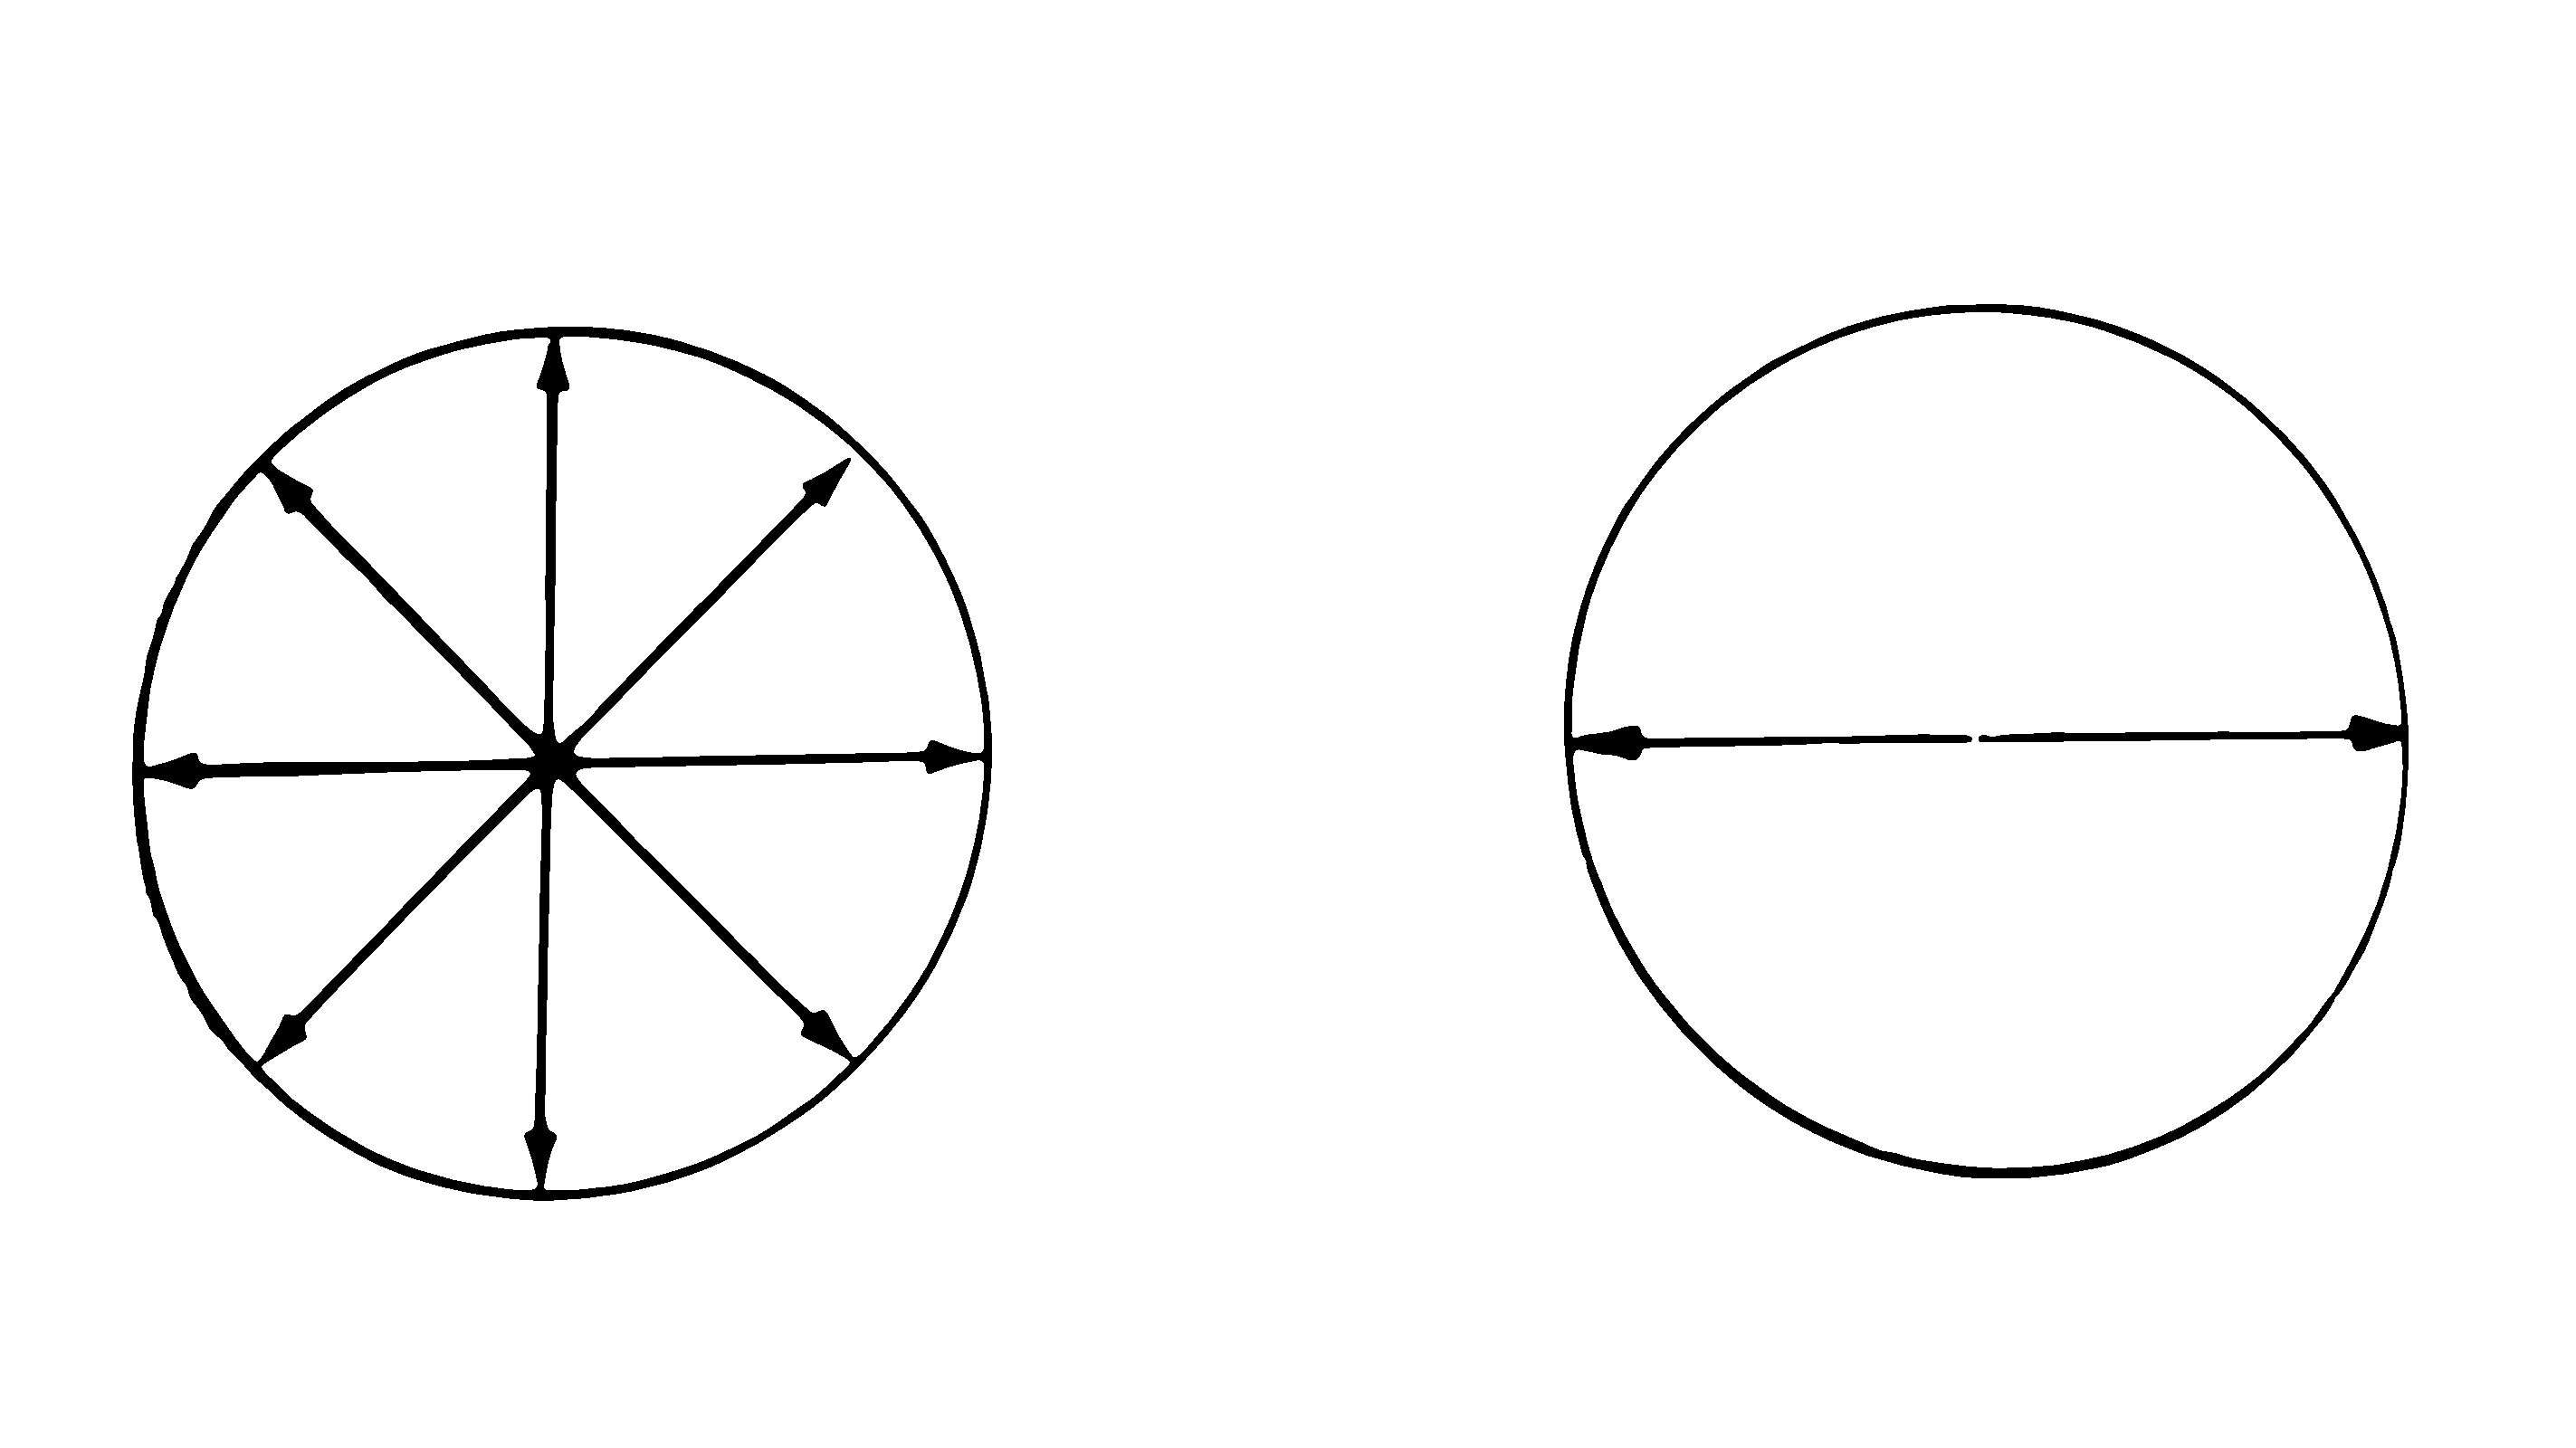
\includegraphics[width=0.5\textwidth,angle=0]{content/images/Figura_6_1.pdf}
    \caption{Vetores elétricos de um feixe de lux comum (esquerda) e polarizada (direita).}
    \label{figura_6_1}
\end{figure}

A luz polarizada (ou, mais propriamente, plano-polarizada) é aquela em que um dos vetores componentes foi removido. A vibração electromagnética resultante está, portanto, em um plano bem definido. Existem inúmeros modos de se conseguir este tipo de polarização um dos quais se utiliza do \textit{prisma de Nicol}. Esse tipo de prisma divide a luz ordinária incidente em dois feixes polarizados em planos perpendiculares.

A Figura \ref{figura_6_2} mostra, esquematicamente, um polarímetro. A luz monocromática ordinária (usualmente luz monocromática de sódio) entra através de um prisma (o polarizador) e é convertida em luz plano-polarizada que atravessa a célula de amostra e chega a outro prisma de Nicol, o chamado \textit{analisador}. Se não há amostra no tubo, a luz polarizada guarda seu aparelho e sua orientação fixa o plano que serve de origem aos ângulos. O prisma analisador pode ser girado à vontade e quando atinge a orientação adequada, toda a luz que a ele chega é capaz de atravessá-lo. A noventa graus dessa orientação a luz não pode atravessá-lo por não estar vibrando neste plano e o campo do visor fica escuro. Para rotações entre estas duas situações a luz é parcialmente transmitida. Os ângulos correspondentes podem ser lidos em um dispositivo semelhante a um transferidor.

\begin{figure}
    \centering
    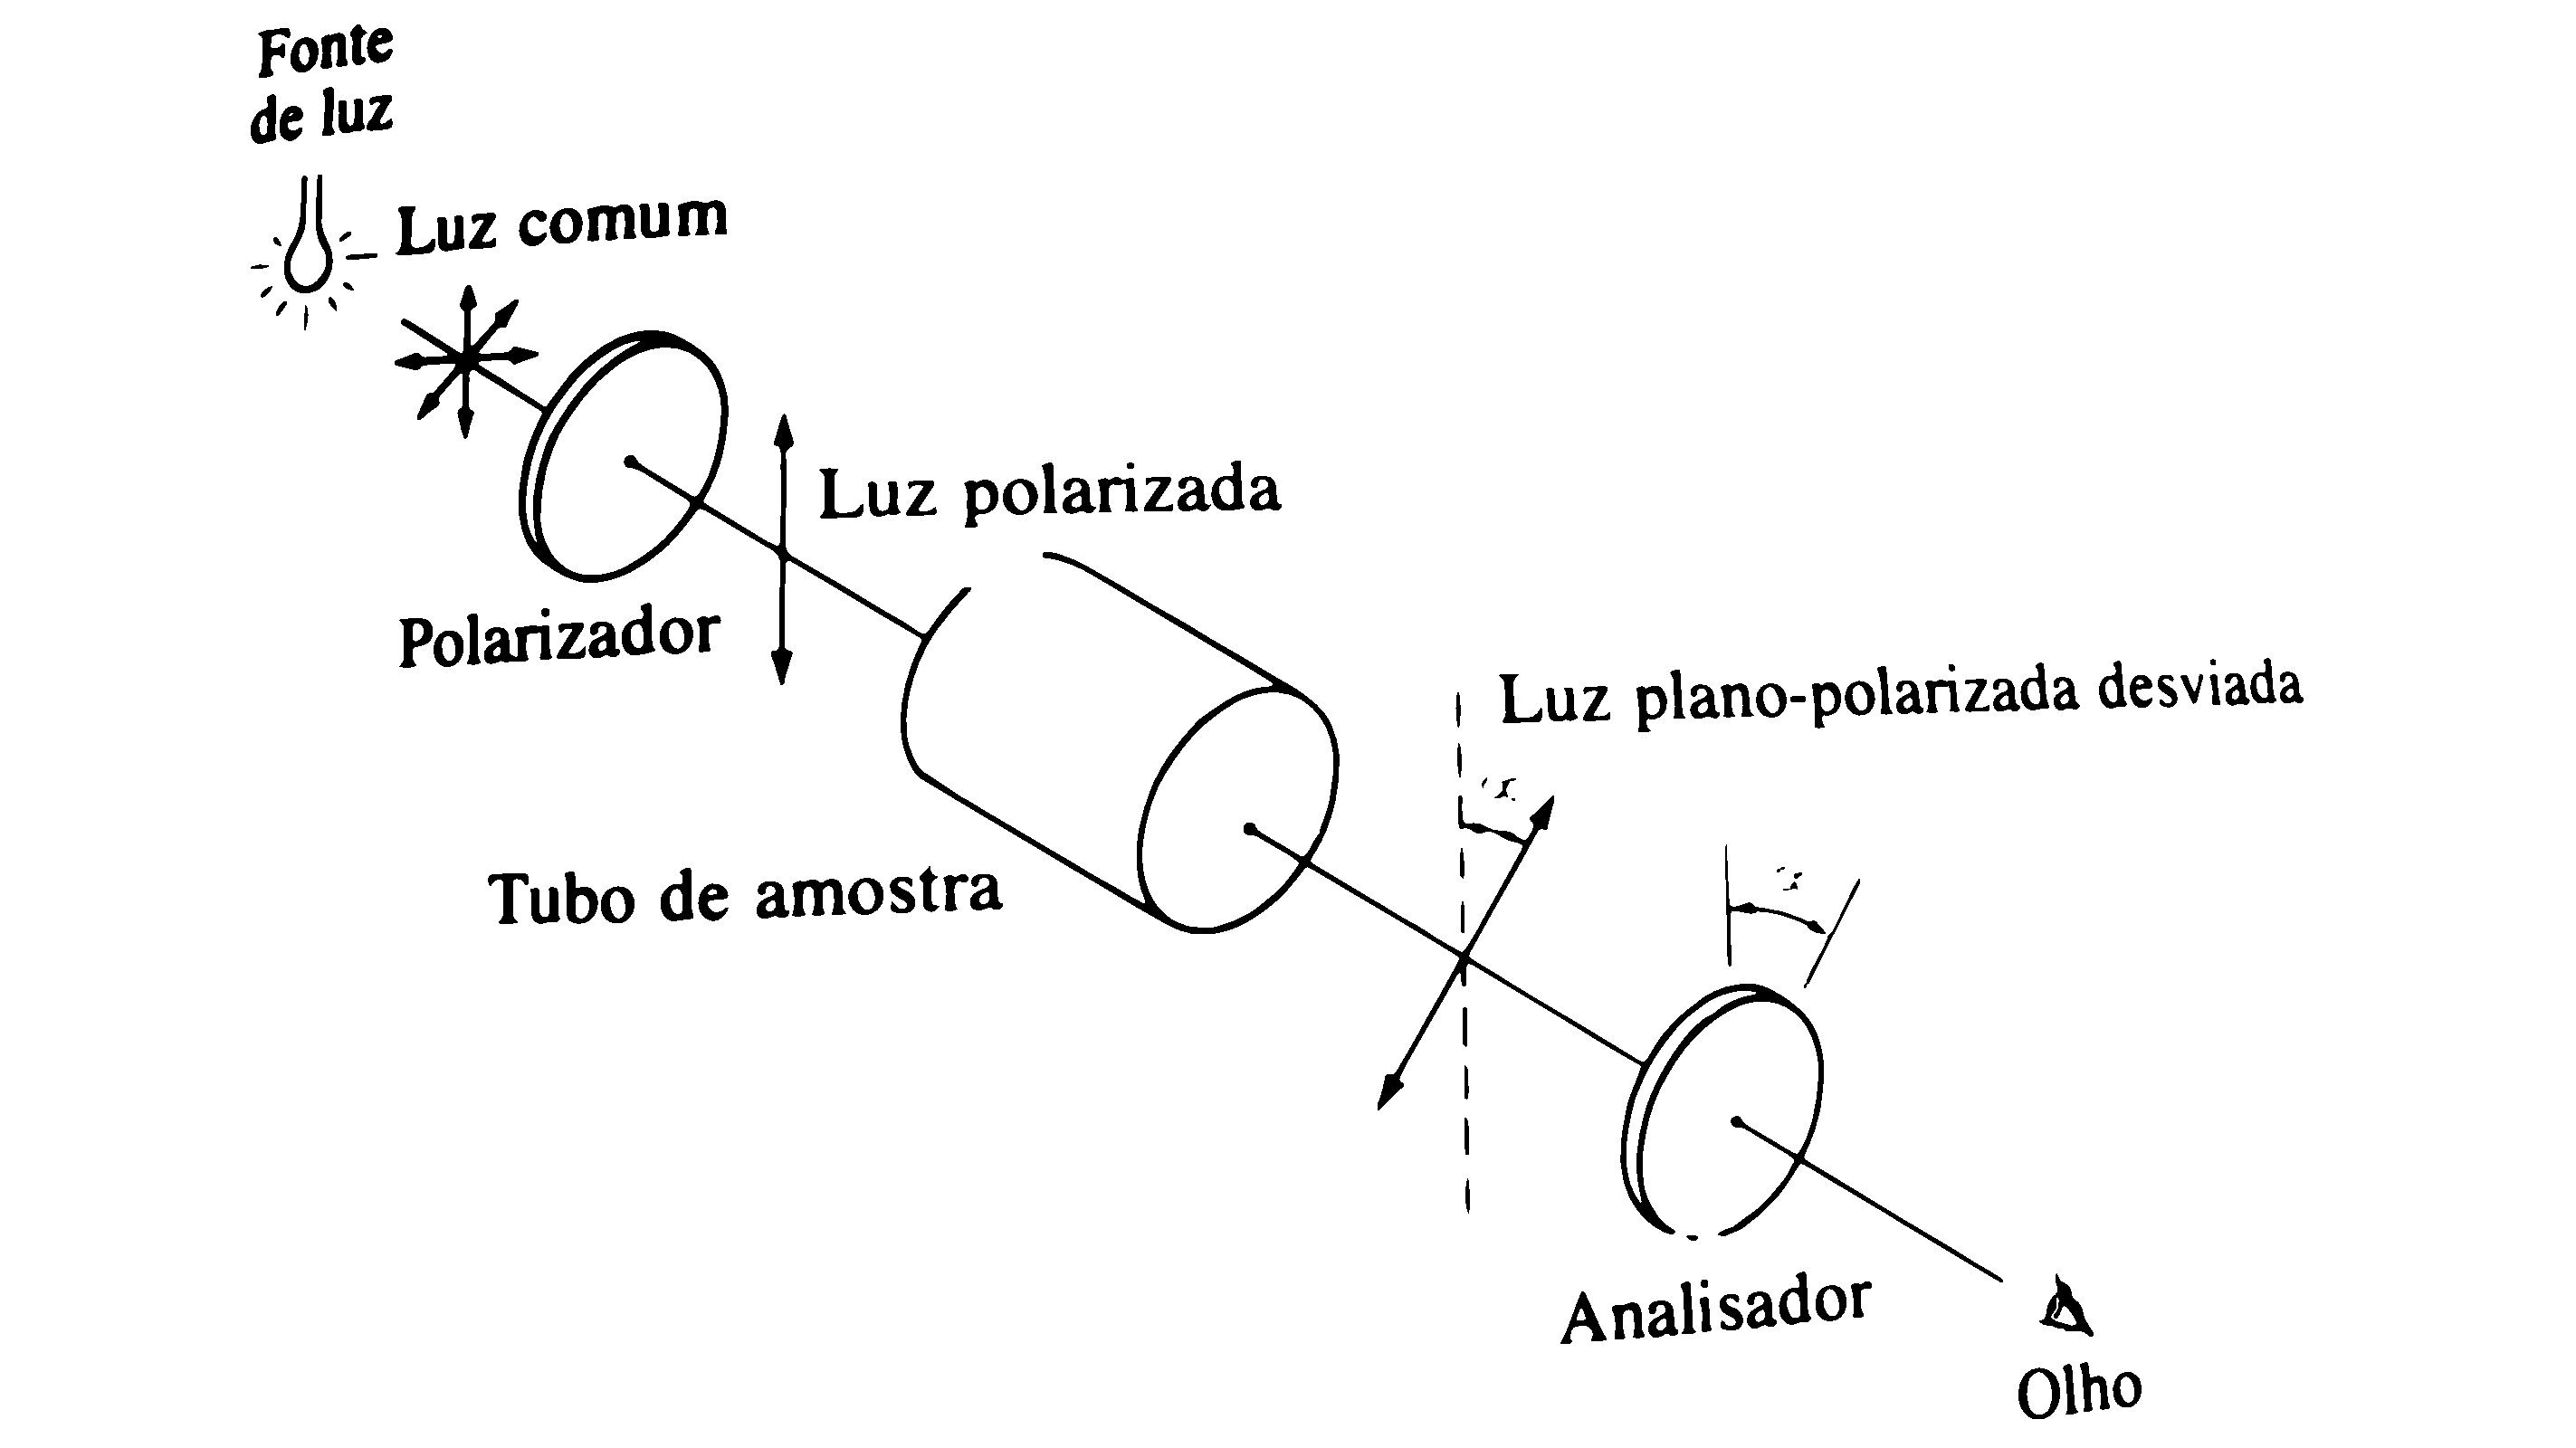
\includegraphics[width=0.7\textwidth,angle=0]{content/images/Figura_6_2.pdf}
    \caption{Representação esquemática de um polarímetro.}
    \label{figura_6_2}
\end{figure}

Quando o tubo de amostra está vazio, o máximo de luz transmitida ocorre para um angulo de rotação do analisador do 0$\degree$. Se substâncias comuns, como a água ou solução salina, são colocadas no tubo de amostra, o máximo de transmissão ainda coincide com a rotação de 0$\degree$ do analisado. Para certas outras substâncias, contudo, ocorre diferentemente. Por exemplo, para uma solução de açúcar,  o analisador tem de sair da posição de 0$\degree$, para que se possa observar um máximo na transmitância. O valor dessa rotação depende da concentração da solução, do comprimento do tubo de amostra, da temperatura, do comprimento de onda da luz utilizada e do solvente.

Para comparar com precisão as medidas de polarizada ode varias amostras, todas as variáveis têm de ser especificadas. Para converter as medidas a uma base mais sistemática, define-se uma quantidade chamada \textit{rotação especifica}, [$\alpha$]. como sendo a rotação em graus produzida em luz plano-polarizada por 1 g de substância em 1 mL de solução quando o comprimento da célula é de 1 decímetro. O valor da rotação, que pode ser direta (sentido dos ponteiros do relógio, positiva) ou inversa (sentido oposto, negativa), é, então, uma característica do composto examinado, desde que as demais variáveis sejam mantidas constantes.

\begin{equation}
    [\alpha] = \dfrac{\text{rotação observada}}{\text{comprimento do tubo (dm)} \times \text{concentração (g$\cdot$mL$^{-1}$)}}
\end{equation}

\noindent A linha $D$ do sódio (a linha de 5893 \AA, que dá a cor amarela à chama do sódio) é a fonte luminosa mais frequentemente usada e a temperatura mais comum é 25$\degree$C. A notação $[\alpha]_D$ fornece essas informações. Uma vez que a rotação especifica depende do solvente e da concentração (neste caso em gramas por 100 mL), é costume especificar a concentração e o solvente em seguida ao valor de $[\alpha]_D$. Por exemplo:

\begin{equation}
    [\alpha]_D = -32.3 \degree \enspace \text{\ch{CHCl3}} \enspace (c \enspace 2.05)
\end{equation}

\section{ENANTIÔMEROS E MISTURAS RACÊMICAS}

A interpretação correta do fenômeno da atividade ótica foi feita independentemente, por van't Hoff, na Holanda, e Le Bel, em Paris, em 1874. Os fatos experimentais exigem que se postule a geometria de um tetraedro regular para o átomo de carbono. Esta geometria, por outro lado, explica plenamente os fatos experimentais. Antes dessa época os químicos consideravam impossível saber qualquer coisa a respeito do arranjo especial das estruturas das moléculas - por arranjo espacial da estrutura entendemos a ordem em que os átomos se combinam para formá-la.

As propriedades geométricas do tetraedro são tais que, se houver quatro substituintes \textit{diferentes} ligados ao átomo de carbono, a molecular não conterá nenhum plano de simetria e isto acarreta a existência de dois arranjos geométricos diferentes para os quatro grupos ligados ao carbono. A diferença entre estes dois arranjos (\textit{configurações}) é que as duas estruturas não são superponíveis, átomo por átomo. Na verdade, as duas estruturas são \textit{imagens especulares não superponíveis} uma da outra (Figura \ref{figura_6_3}).

% \begin{figure}[H]
%     \centering
%     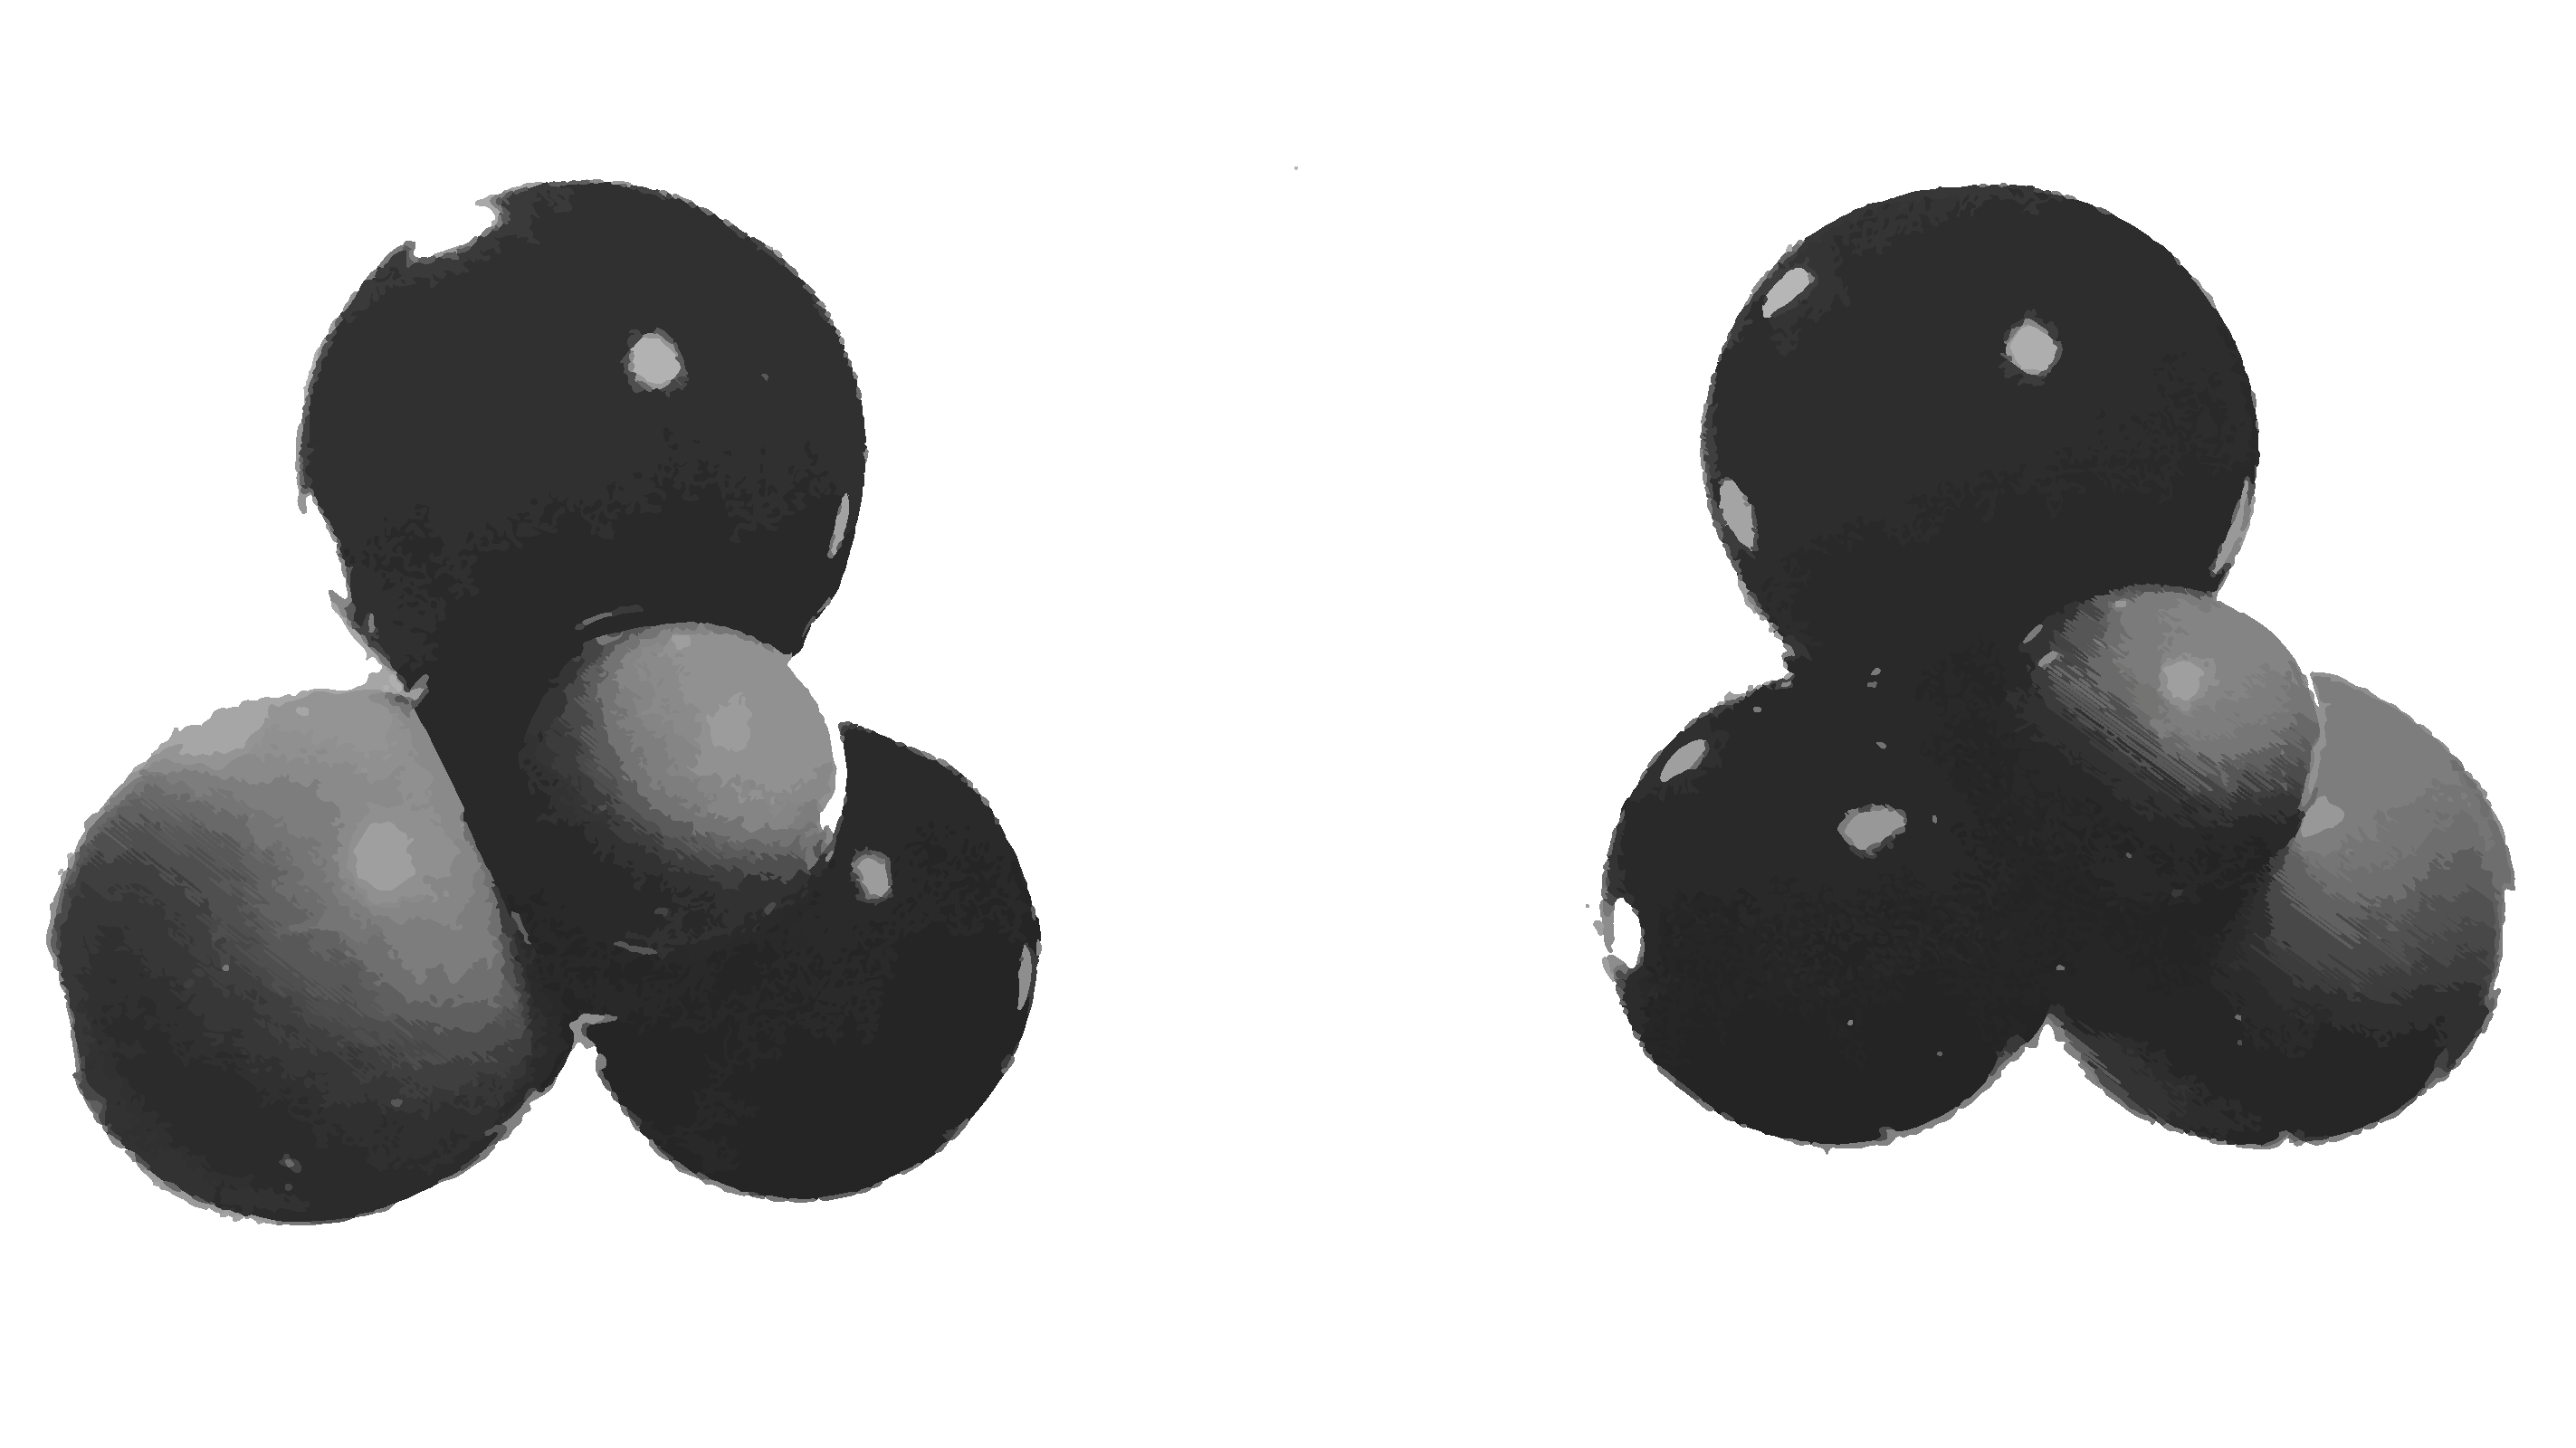
\includegraphics[width=0.5\textwidth,angle=0]{content/images/Figura_6_3.pdf}
%     \caption{Imagens especulares não superponíveis.}
%     \label{figura_6_3}
% \end{figure}

\begin{figure}[H]
    \centering
    \begin{tikzpicture}[help lines/.style={thin,draw=black!50}] 
        %\draw[help lines] (0,0) grid (12,4);
        \shade[ball color = black] (2,3) circle (0.8cm);
        \draw[thick] (2,3) circle (0.8cm);
        \shade[ball color = black] (2.9,1.9) circle (0.7cm);
        \draw[thick] (2.9,1.9) circle (0.7cm);
        \shade[ball color = gray!40] (1.5,1.5) circle (0.8cm);
        \draw[thick] (1.5,1.5) circle (0.8cm);
        \shade[ball color = gray!40] (2.3,2) circle (0.6cm);
        \draw[thick] (2.3,2) circle (0.6cm);
        \begin{scope}[xscale=-1,xshift=-8cm]
            \shade[ball color = black] (2,3) circle (0.8cm);
            \draw[thick] (2,3) circle (0.8cm);
            \shade[ball color = black] (2.9,1.9) circle (0.7cm);
            \draw[thick] (2.9,1.9) circle (0.7cm);
            \shade[ball color = gray!40] (1.5,1.5) circle (0.8cm);
            \draw[thick] (1.5,1.5) circle (0.8cm);
            \shade[ball color = gray!40] (2.0,2) circle (0.6cm);
            \draw[thick] (2.0,2) circle (0.6cm);
        \end{scope}
    \end{tikzpicture}
    \caption{Imagens especulares não superponíveis.}
    \label{figura_6_3}
\end{figure}

\noindent Tais moléculas resultam da ligação de quatro grupos diferentes ao carbono e são chamadas de \textit{assimétricas} ou, então, de moléculas que contêm um \textit{carbono assimétrico}.

\begin{figure}[H]
    \centering
    \chemfig[][scale=0.7]{[1]d>(-[2]a)(<[7]c)(<:[6]b)}
    \qquad\qquad
    \chemfig[][scale=0.7]{[1]c>(-[2]a)(<[7]d)(<:[6]b)}
\end{figure}

\noindent\emph{No decorrer do texto adotaremos a seguinte convenção. A ligação que está no plano do papel é indicada por um traço fino, as que estão para a frente do plano são indicadas por uma cunha em negrito: finalmente, as que estão para trás são indicadas por uma cunha tracejada. Reservaremos o uso de uma linha fina tracejada para indicar outras ideias, como, por exemplo, que uma ligação está parcialmente rompida.}

Se dois compostos são imagem especular não superponível um do outro são chamados de \textit{enanciômeros}. Encontra-se experimentalmente que os enanciômeros possuem propriedades físicas idênticas., como era de se esperar, exceto a de rotação da luz polarizada, que é feita em direções opostas (e pelo mesmo ângulo). O 2-cloro-butano é um exemplo desta situação, já que existe como um par de enanciômeros.

\begin{figure}[H]
    \centering
    \begin{tikzpicture}[help lines/.style={thin,draw=black!50}] 
        %\draw[help lines] (0,0) grid (4,4);
        \draw[dashed,thick] (2,1) node[yshift=-2ex] {\footnotesize{Imagens especulares não superponíveis}} -- (2,3) node[yshift=2ex] {\footnotesize{Plano do espelho}};
        \node at (0,2) {\chemfig[][scale=0.7]{C_2H_5>C(<:[1]H)(<:[7]Cl)(<CH_3)}};
        \node at (4,2) {\chemfig[][scale=0.7]{CH_3>C(<:[1]H)(<:[7]Cl)(<C_2H_5)}};
    \end{tikzpicture}
\end{figure}

\noindent O leitor deveria construir modelos destes enanciômeros e convencer-se de que eles não são superponíveis.

Se dois enanciômeros são misturados em quantidades iguais, o resultado é o que chamamos de \textit{mistura racêmica}, que não muda o plano da luz polarizada porque o desvio de cada enanciômeros cancela o do outro. 

Cotidianamente deparamos com uma série de enanciômeros. Por exemplo, a mão esquerda é a imagem especular da mão direita, e as duas mãos, como bem o sabemos, não se superpõem. Isso fica obvio quando tentamos vestir uma luva de mão direita na mão esquerda. Da mesma forma, nossos sapatos guardam entre si uma relação enanciomérica e o estoque de uma sapataria exemplifica uma mistura racêmica.

Se a molécula é superponível à sua imagem especular (molécula e imagem são idênticas), tal substância não pode existir como um par de enanciômeros, e sim como um composto que não desvia o plano da luz polarizada. Com moléculas simples, é fácil determinar se a atividade ótica será observada ou não. Se dois ou mais átomos ou grupos de átomos ligados ao carbono são iguais, então não haverá carbono assimétrico, as imagens especulares serão superponíveis e as estruturas correspondentes serão idênticas, isto é, a mesma molécula. O 2-cloro-propano exemplifica isto.

\begin{figure}[H]
    \centering
    \begin{tikzpicture}[help lines/.style={thin,draw=black!50}] 
        %\draw[help lines] (0,0) grid (4,4);
        \draw[dashed,thick] (2,1) node[yshift=-2ex] {\footnotesize{Imagens especulares superponíveis}} -- (2,3) node[yshift=2ex] {\footnotesize{Plano do espelho}};
        \node at (0,2) {\chemfig[][scale=0.7]{CH_3>C(<:[1]H)(<:[7]Cl)(<CH_3)}};
        \node at (4,2) {\chemfig[][scale=0.7]{CH_3>C(<:[1]H)(<:[7]Cl)(<CH_3)}};
    \end{tikzpicture}
\end{figure}

\noindent Comparemos esse composto com o 2-cloro-butano em que todos os grupos ligados ao carbono 2 são diferentes. Em compostos simples, a presença de um átomo de carbono assimétrico levará à existência de enanciômeros.

Vale a pena perguntar se os isômeros óticos não passam de curiosidade acadêmica ou se eles têm importância no nosso mundo real. Como ficará claro em capítulos posteriores, muitos, e na, verdade a maioria, dos compostos que ocorrem em sistemas vivos contêm um ou mais átomos de carbono assimétrico. Os sistemas biológicos são particularmente exigentes em relação aos isômeros óticos que preferem e é de suma importância compreender este fenômeno se quisermos compreender os sistemas vivos.

\noindent\emph{Também podemos perguntar: Por que os enanciômeros comportam-se desta maneira em relação à luz polarizada? Se examinarmos uma solução de um composto, um líquido ou gás puros, por exemplo metano, verificamos que eles contêm moléculas orientadas de todos os modos possíveis. Uma dada molécula em uma orientação arbitrariamente fixada desviara o plano de polarização de luz de um pequeno ângulo, digamos, para a esquerda. Se a molécula é superponível à sua imagem especular, como é o caso do metano, é igualmente provável que a luz venha encontrar outra molecular com uma orientação correspondente à imagem especular da primeira em um dado instante do percurso. As contribuições rotacionais das duas moléculas serão, então, iguais, opostas e se cancelarão. Ao trabalharmos com uma amostra macroscópica as varias orientações possíveis desviarão o plano de rotação da luz com diferentes intensidades e em diferentes direções, mas as compensações farão com que a rotação total seja sempre zero na média.}

\emph{Se dispusermos, por outro lado, de uma solução composta de moléculas idênticas, porém não superponíveis a suas imagens especulares, correspondendo a um mesmo enanciômero, cada molécula poderá estar em diferentes orientações de modo que cada uma contribuirá para a rotação ótica da solução como um todo. Mas como a imagem especular de cada orientação corresponde ao enanciômero que não está presente, as rotações não se cancelam, somando-se para dar como resultado um valor qualquer diferente de zero. O outro enanciômero em solução teria um comportamento correspondente e, portanto, um desvio de igual angulo em sentido oposto. Uma mistura constituída de quantidades iguais orientação, haveria uma probabilidade igual de ocorrência de sua imagem especular e a rotação resultante de tal mistura seria zero.}

\section{PROJEÇÕES DE FISCHER}

É difícil fazer a representação tridimensional de um tetraedro com um desenho ou uma formula a duas dimensões. As duas representações adequadas são as \textit{formulas em perspectiva} (Seção 3.1) e de \textit{projeção}. No presente texto usaremos ambas. As formulas de projeção mostram apenas duas dimensões, sendo a terceira perpendicular ao pano do papel. As \textit{projeções de Fischer} são bastante usadas por causa de sua simplicidade (Figura \ref{figura_6_4}).

\begin{figure}[H]
    \centering
    \begin{tikzpicture}[help lines/.style={thin,draw=black!50}] 
       % \draw[help lines] (0,0) grid (12,4);
        \shade[ball color = gray!40, opacity = 0.4] (2,2) circle (0.3cm);
        \draw[thick] (2,2) circle (0.3cm);
        \draw (3.5,2) circle (0.35cm) node {$b$};
        \draw (0.5,2) circle (0.35cm) node {$a$};
        \draw (2,3.5) circle (0.25cm) node {$c$};
        \draw (2,0.5) circle (0.25cm) node {$d$};
        \draw[rounded corners=1pt] (2.1,1.72) -- (2.03,0.6) -- (1.97,0.6) -- (1.9,1.72);
        \draw[rounded corners=1pt] (2.1,2.28) -- (2.03,3.4) -- (1.97,3.4) -- (1.9,2.28);
        \path[draw,fill=white] (2.1,1.68) -- (2.03,0.6) -- (1.97,0.6) -- (1.9,1.68);
        \path[draw,fill=white] (2.1,2.32) -- (2.03,3.4) -- (1.97,3.4) -- (1.9,2.32);
        \draw[rounded corners=1pt] (0.83,2.1) -- (1.90,2.03) -- (1.90,1.97) -- (0.83,1.9);
        \draw[rounded corners=1pt] (3.17,2.1) -- (2.10,2.03) -- (2.10,1.97) -- (3.17,1.9);
        \path[draw,fill=white] (0.88,2.1) -- (1.90,2.03) -- (1.90,1.97) -- (0.88,1.9);
        \path[draw,fill=white] (3.12,2.1) -- (2.10,2.03) -- (2.10,1.97) -- (3.12,1.9);
        \node at (6,2) {\chemfig[][scale=0.7]{a>(<:[2]c)(<:[6]d)<b}};
        \node at (4,0) {\footnotesize{Fórmulas em perspectiva}};
        \node at (9,2) {\chemfig[][scale=0.7]{a-C(-[2]c)(-[6]d)-b}};
        \node at (9,0) {\footnotesize{Fórmula de projeção}};
        \node at (12,2) {\chemfig[][scale=0.7]{d-(-[2]a)(-[6]b)-c}};
        \node at (12,0) {\footnotesize{Projeção de Fischer}};
    \end{tikzpicture}
    \caption{Quatro representações equivalentes de um carbono tetraédrico.}
    \label{figura_6_4}
\end{figure}

Por convenção, as linhas horizontais são imaginadas para cima do plano da página, enquanto que as verticais são entendidas como ligações que se dirigem para baixo do papel. Manipulemos agora algumas destas fórmulas para mostrar claramente o que representam.

\begin{figure}[H]
    \centering
    \schemestart
        \chemfig[][scale=0.7]{a-(-[2]c)(-[6]d)-b}
        \qquad\text{\footnotesize{e}}\qquad
        \chemfig[][scale=0.7]{b-(-[2]d)(-[6]c)-a}
    \schemestop
\end{figure}

\noindent Em uma projeção de Fischer, as duas formulas referem-se à mesma molécula. É fácil vermos porque, desenhando as duas fórmulas em perspectiva correspondentes:

\begin{figure}[H]
    \centering
    \schemestart
        \chemfig[][scale=0.7]{a>(<:[2]c)(<:[6]d)<b}
        \qquad\text{\footnotesize{e}}\qquad
        \chemfig[][scale=0.7]{b>(<:[2]d)(<:[6]c)<a}
    \schemestop
\end{figure}

\noindent Se tomarmos a segunda fórmula e a rodarmos de 180$\degree$ no sentido direto, mantendo-a no plano da página.

\begin{figure}[H]
    \centering
    \schemestart
        \chemfig[][scale=0.7]{@{a2}b>(<:[2]d)(<:[6]c)<a@{a1}}
        \arrow{->}
        \chemfig[][scale=0.7]{a>(<:[2]c)(<:[6]d)<b}
    \schemestop
    \chemmove{\draw(a1).. controls +(south:1.2cm) and +(south:1.2cm).. (a2);}
\end{figure}

\noindent veremos que $a$ e $b$ mudaram de lugar, assim como $c$ e $d$, e que $a$ e $b$ ainda se projetam em nossa direção e $c$ e $d$ para trás do papel. Note que o que conseguimos com esta operação foi colocar a estrutura em uma situação idêntica à da primeira. A conclusão é que as duas fórmulas em perspectiva representam, neste caso, o mesmo composto. 

Vales a pena lembrar que a rotação de 180$\degree$ imposta a uma projeção de Fischer leva sempre à outra projeção, a qual corresponde a uma molécula idêntica. Por outro lado, as duas projeções de Fischer que se seguem não são idênticas e representam um par de enanciômeros:

\begin{figure}[H]
    \centering
    \schemestart
        \chemfig[][scale=0.7]{a-(-[2]c)(-[6]d)-b}
        \qquad\text{\footnotesize{e}}\qquad
        \chemfig[][scale=0.7]{d-(-[2]a)(-[6]b)-c}
    \schemestop
\end{figure}

\noindent Para demonstrar essa afirmativa escrevemos outra vez as fórmulas em perspectiva correspondentes:

\begin{figure}[H]
    \centering
    \schemestart
        \chemfig[][scale=0.7]{a>(<:[2]c)(<:[6]d)<b}
        \qquad\text{\footnotesize{e}}\qquad
        \chemfig[][scale=0.7]{d>(<:[2]a)(<:[6]b)<c}
    \schemestop
\end{figure}

\noindent Para tentar superpô-las, tomamos a segunda estrutura e rodamos 90$\degree$ no sentido inverso, realizando a rotação no plano da página:

\begin{figure}[H]
    \centering
    \schemestart
        \chemfig[][scale=0.7]{d>(<:[2]a@{a2})(<:[6]b)<c@{a1}}
        \arrow{->}
        \chemfig[][scale=0.7]{a>:(<[2]c)(<[6]d)<:b}
    \schemestop
    \chemmove{\draw(a1).. controls +(90:0.5cm) and +(45:0.5cm).. (a2);}
\end{figure}

Se compararmos agora a estrutura obtida com a premeria, podemos ver que os grupos estão ligados ao carbono assimétrico na mesma ordem, em outras palavras, começando com o grupo $a$, no sentido direto a ordem é $acbd$, em ambas as estruturas. Porém os grupos que vice-versa. Isto significa que as duas estruturas aparecem acima do plano na outra estrutura e sendo o plano do papel o plano do espelho. Portanto, as fórmulas de projeção que escrevemos representam um par de enanciômero e têm configurações opostas em torno do átomo de carbono assimétrico. 

O método acima pode ser sempre usado para se descobrir se duas projeções de Fischer correspondem à mesma molécula ou a enanciômeros. Entretanto, essa verificação é bastante laboriosa e leva facilmente a erro. Para simplificar a questão os químicos desenvolveram uma regra simples: para um composto que contém apenas um carbono assimétrico \textit{a troca de dois grupos quaisquer na projeção de Fischer converte a molécula no seu enanciômero}. Considere o exemplo abaixo:

\begin{figure}[H]
    \centering
    \schemestart
        \chemfig[][scale=0.7]{a-(-[2]c)(-[6]d)-b}
        \qquad\text{\footnotesize{trocando $a$ por $d$, obtém-se}}\qquad
        \chemfig[][scale=0.7]{d-(-[2]c)(-[6]a)-b}
    \schemestop
\end{figure}

\noindent que é o enanciômero da primeira molécula.

Suponhamos agora que nós tomamos a segunda fórmula e trocamos dois grupos. Isso nos leva ao enanciômero da segunda fórmula, isto é, nos leva de volta à primeira estrutura. Em outras palavras, o que fizemos foi trocar $a$ e $d$ mais uma vez. Podemos trocar, entretanto, \textit{quaisquer} dois grupos para obter um enanciômero. Usemos a segunda fórmula e troquemos dois outros grupos:

\begin{figure}[H]
    \centering
    \schemestart
        \chemfig[][scale=0.7]{d-(-[2]c)(-[6]a)-b}
        \qquad\text{\footnotesize{trocando $a$ por $c$, obtém-se}}\qquad
        \chemfig[][scale=0.7]{d-(-[2]a)(-[6]c)-b}
    \schemestop
\end{figure}


\include{content/Capítulo_7}
\chapter{Grupos Funcionais que Contêm Oxigênio Ligado Duplamente a um Átomo de Carbono: o Grupo Carbonila}

Nos Capítulos 3 e 7 discutimos com algum detalhe as estruturas e propriedades dos alcanos e alquenos. No Capítulo 4 discutimos os compostos que contêm um ou mais heteroátomos em ligações simples. Iniciaremos agora o estudo do grupo de compostos que contêm ligações múltiplas envolvendo heteroátomos. Começaremos pela ligação dupla carbono-oxigênio, retornando ao assunto no Capítulo 10, que introduz outras ligações múltiplas envolvendo heteroátomos.

\section{O GRUPO CARBONILA}

O arranjo \ch{R2C=O} é chamado \textit{grupo carbonila}, e os compostos que contêm este arranjo de átomos são chamados de \textit{compostos carbonilados}. A Figura \ref{figurar_8_1} mostra as estruturas das classes funcionais mais comuns de compostos que contêm o grupo carbonila:


\begin{figure}[H]
    \centering
    \chemnameinit{}
    \chemname{\setchemfig{atom sep=2em}\chemfig{R-C(=[2]O)-H}}{Aldeído}
    \qquad
    \chemname{\setchemfig{atom sep=2em}\chemfig{R-C(=[2]O)-R^1}}{Cetona}
    \qquad
    \chemname{\setchemfig{atom sep=2em}\chemfig{R-C(=[2]O)-OH}}{Ácido carboxílico}
    \qquad\qquad
    \chemname{\chemname{\setchemfig{atom sep=2em}\chemfig{R-C(=[2]O)-OOH}}{Ácido peróxi-carboxílico}}{(Ácido percarboxílico)}
    \par\bigskip
    \begin{flushleft}
        Derivados de ácidos:
    \end{flushleft}
    \par\bigskip
    \chemnameinit{}
    \chemname{\setchemfig{atom sep=2em}\chemfig[][]{R-C(=[2]O)-OR^1}}{Éster}
    \qquad
    \chemname{\setchemfig{atom sep=2em}\chemfig{R-C(=[2]O)-NR^1_2}}{Amida}
    \qquad
    \chemname{\setchemfig{atom sep=2em}\chemfig{R-C(=[2]O)-O-C(=[2]O)-R}}{Anidrido}
    \qquad\qquad
    \chemname{\setchemfig{atom sep=2em}\chemfig{R-C(=[2]O)-X}}{Halogeneto de acila}
    \caption{Classes funcionais que contêm o grupo carbonila.}
    \label{figurar_8_1}
\end{figure}

\noindent Os grupos funcionais têm o nome particular de:

\begin{tightcenter}
    \schemestart
        \chemnameinit{}
        \chemname[4ex]{\setchemfig{atom sep=2em}\chemfig{C(-[3])(-[5])=O}}{Grupo carbonila}
        \qquad\qquad
        \chemnameinit{}
        \chemname[2.5ex]{\setchemfig{atom sep=2em}\chemfig{-C(=[1]O)(-[7]OH)}}{Grupo carboxila}
        \qquad\qquad
        \chemnameinit{}
        \chemname[1.9ex]{\setchemfig{atom sep=2em}\chemfig{-C(=[1]O)(-[7]O^{-})}}{Íon carboxilato}
        \qquad\qquad
        \chemname[2.3ex]{\setchemfig{atom sep=2em}\chemfig{R-C(=[2]O)-}}{Grupo acila}
    \schemestop
\end{tightcenter}

O composto carbonilado mais simples é o formaldeído, \ch{H2CO}, um gás muito solúvel em água. Os compostos carbonilados de baixo peso molecular são líquidos. Os ésteres têm odor de frutas, e as cetonas cíclicas grandes têm odor muito agradável, sendo, habitualmente, componentes de perfumes de alto preço. Os ácidos carboxílicos, anidridos e halogenetos de acila têm, geralmente, odores desagradáveis. 

A ligação \ch{C=O} em compostos das classes apresentadas na Figura \ref{figurar_8_1} é, do mesmo modo que a ligação \ch{C=C} de olefinas, composta por uma ligação $\sigma$ e uma ligação $\pi$. O grupo carbonila pode ser representado como sendo formado pelo entrosamento de um orbital $sp^2$ do carbono com um orbital $2p_x$ do oxigênio para formar a ligação $\sigma$ e pelo entrosamento lateral dos orbitais $2p_z$ do carbono e do oxigênio para formar uma ligação $\pi$ (Figura \ref{figura_8_2}). Há um par de elétrons livres no orbital $2s$ e outro par no orbital $2p_y$ do oxigênio.

\begin{figure}[H]
    \centering
    \begin{tikzpicture}[help lines/.style={thin,draw=black!50}] 
        %\draw[help lines] (0,0) grid (7,7);
        \path (2,3.2) node (m) {C} ($ (m) + (350:2) $) node (o) {O};
        \path ($ (m) + (90:0.9) $) node (ma) {} ($ (o) + (90:0.9) $) node (oa) {};
        \draw[] (m) -- ++(270:2);
        \draw[] (m) -- ++(90:1);
        \draw[] (o) -- ++(270:2);
        \draw[] (m) -- ++(170:1);
        \draw[dashed] (m) -- (o);
        \draw[] (o) -- ++(90:1);
        \draw[] (m) -- ++(30:2);
        \draw[] (o) -- ++(30:2);
        \draw[] (m) -- ++(210:2);
        \draw[] (o) -- ++(210:2) node[align=center] {\enspace\enspace\footnotesize{y}};
        
        \filldraw[fill=white,thick] ($ (m) + (90:0.8) $) ellipse (0.6 and 0.4);

        \draw[->,>=stealth] (ma) -- ++(90:1);

        \filldraw[fill=white,thick] ($ (m) + (270:0.8) $) ellipse (0.6 and 0.4);

        \filldraw[fill=white,thick] ($ (o) + (30:0.8) $) ellipse (0.4 and 0.6);

        \draw[->,>=stealth] (o) -- ++(350:1.5) node[align=right] {\enspace\footnotesize{x}};

        \filldraw[fill=white,thick] ($ (o) + (90:0.8) $) ellipse (0.6 and 0.4);

        \draw[->,>=stealth] (oa) -- ++(90:1) node[align=right] {\enspace\enspace\footnotesize{z}};

        \filldraw[fill=white,thick] ($ (o) + (270:0.8) $) ellipse (0.6 and 0.4);

        \node (t1) at ($ (m) + (90:1) $) {};
        \node (t2) at ($ (o) + (90:1) $) {};
        \node (b1) at ($ (m) + (270:1) $) {};
        \node (b2) at ($ (o) + (270:1) $) {};
        \draw[dashed] (t1) -- (t2);
        \draw[dashed] (b1) -- (b2);

        \filldraw[fill=white,thick] ($ (o) + (210:0.8) $) ellipse (0.4 and 0.6);
    \end{tikzpicture}
    \caption{Grupo carbonila planar com o oxigênio ($p^3$) não-hibridado. Não aparece o par de elétrons livres do orbital $2s$ do oxigênio.}
    \label{figura_8_2}
\end{figure}

A ligação \ch{C=O} é uma ligação muito forte, 176-179 kcal mol$^{-1}$, um pouco mais forte do que duas ligações \ch{C-O} (2 $\times$ 85,5 kcal mol$^{-1}$) mas, apesar disto, é uma ligação dupla muito reativa. A alta reatividade é devida à diferença de eletronegatividade entre o carbono e o oxigênio, que leva a uma contribuição importante da forma de ressonância polar na qual o oxigênio é negativo e o carbono positivo. Estudos de momento de dipolo indicam que a contribuição da forma polar pode chegar a 50 por cento:

\begin{tightcenter}
\schemestart
    \setchemfig{atom sep=2em}\chemfig[][]{C(-[3])(-[5])=\lewis{0:6:,O}}
    \qquad\arrow{<->}
    \setchemfig{atom sep=2em}\chemfig[][]{\chemabove{C}{\hspace{+5mm}\scriptstyle +}(-[3])(-[5])=\lewis{0:2:6:,\chemabove{O}{\hspace{+5mm}\scriptstyle -}}}
\schemestop
\end{tightcenter}

Em compostos nos quais o átomo ligado ao grupo carbonila tem orbitais $p$ ocupados, a ligação é complicada pela possibilidade de deslocalização adicional dos elétrons (ressonância). 

\begin{tightcenter}
\schemestart
    \setchemfig{atom sep=2em}\chemfig[][]{-C(=[1]\lewis{0:2:,O})(-[7]\lewis{0:4:6:,Y})}
    \qquad\arrow{<->}
    \setchemfig{atom sep=2em}\chemfig[][]{-C(=[1]\lewis{0:2:6:,\chemabove{O}{\hspace{+5mm}\scriptstyle -}})(-[7]\lewis{0:6:,\chemabove{Y}{\hspace{+5mm}\scriptstyle +}})}
\schemestop
\end{tightcenter}

\noindent A importância da forma dipolar aumenta quando eletronegatividade de Y decresce na ordem halogênio, oxigênio, nitrogênio. Observe que, quando a contribuição da forma dipolar aumenta, o caráter de ligação dupla do grupo carbonila diminui.

Um sistema $\pi$ de quatro centros é possível quando Y é um grupo vinda.

\begin{tightcenter}
\schemestart
    \setchemfig{atom sep=2em}\chemfig[][]{-C(=[2]O)-CH=CH-}
    \arrow{<->}
    \setchemfig{atom sep=2em}\chemfig[][]{-C(-[2]O)=CH-\chemabove{C}{\scriptstyle +}H-}
\schemestop
\end{tightcenter}

Em uma estrutura deste tipo, as ligações duplas são conjugadas como as do butadieno. O leitor deve voltar a este assunto (Seções 7.12 e 7.13). 

\section{ACIDEZ E BASICIDADE DE COMPOSTOS CARBONILADOS}

\noindent\textbf{O grupo carbonila como ácido de Lewis}

Há muitos compostos orgânicos nos quais um átomo em ligação múltipla pode aceitar parcialmente um par de elétrons, geralmente com o deslocamento síncrono de elétrons na ligação múltipla. (O caso no qual uma ligação múltipla \textit{doa} um par compartilhado de elétrons foi discutido na Seção 7.15.) Podemos adicionar à nossa lista anterior de ácidos de Lewis (Seção 4.1) \textit{os grupos contendo ligações múltiplas possuindo uma região de baixa densidade eletrônica}. 



Observe que o átomo com o qual a base se coordena não tem um orbital vazio, porém um orbital fica disponível pelo deslocamento de elétrons. O mais importante destes ácidos de Lewis é o grupo carbonila. As reações de grupos carbonila como ácidos de Lewis, envolvendo adições à ligação \ch{C=O}, estão entre as mais importantes da química orgânica.




Uma classificação importante das reações iônicas de moléculas orgânicas é baseada na descrição do reagente "que ataca". Pela definição de Lewis, um ácido é qualquer espécie capaz de aceitar um par de elétrons e uma base é um doador de par de elétrons. Os reagentes que são ávidos por elétrons (e, portanto, ácidos de Lewis) são chamados \textit{eletrófilos} (que gostam de elétrons) e os reagentes que são doadores de elétrons (e, portanto, bases de Lewis) são chamados \textit{nucleófilos} (que gostam de núcleos). As reações iônicas são, em consequência, classificadas como \textit{eletrofílicas} ou \textit{nucleofílicas}, de acordo com o tipo de reagente envolvido. Por exemplo, a equação anterior descreve uma \textit{adição nucleofílica} ao grupo carbonila. 

Estas palavras, um tanto elegantes, descreveriam uma situação nova? A resposta é sim. A \textit{basicidade} é medida em termos da posição de \textit{equilíbrio} entre um doador de elétrons e um ácido (geralmente o próton). A \textit{nucleofilia}, por outro lado, é medida em termos da \textit{velocidade} da reação do nucleófilo com o substrato. (A palavra \textit{substrato} é um termo geral para a molécula que está participando da reação em questão.) Considere os exemplos do íon metóxido, \ch{CH3O^{-}}, e do metil-mercapteto, \ch{CH3S^{-}}. Metóxido é a base mais forte, mas o mercapteto é o nucleófilo mais potente. Falaremos mais sobre basicidade e nucleofilia nos próximos capítulos.

\noindent\textit{Bases}
\begin{tightcenter}
    \schemestart
        \ch{CH3O- + H2O}
        \arrow{<->>}
        \ch{CH3OH + HO-}
    \schemestop\par\bigskip
    \schemestart
        \ch{CH3S- + H2O}
        \arrow{<<->}
        \ch{CH3SH + HO-}
    \schemestop
\end{tightcenter}

\noindent\textit{Nucleófilos}

É fácil observar que os ácidos práticos e de Lewis são, ambos, catalisadores eficientes em adições nucleofílicas ao grupo carbonila.



A forma protonada da carbonila tem mais carga positiva no carbono do que a carbonila original, como mostramos. O ataque por um nucleófilo é, assim, facilitado.

\noindent\textbf{O grupo carbonila como base de Lewis} 

O oxigênio do grupo carbonila possui dois pares de elétrons livres e, além disto, uma boa parte da densidade eletrônica dos elétrons ligantes $\sigma$ e $\pi$. Em consequência, o oxigênio funciona como base de Lewis, embora seja $10^{12}$ a $10^{18}$ vezes menos básico do que o nitrogênio de uma amina. 


Deste modo, enquanto a maior parte dos compostos carbonilados, exceto os de peso molecular muito baixo, é insolúvel em água, eles se dissolvem em \ch{H2SO4} concentrado, com a formação de \ch{R2C=OH+}. 

\noindent\textbf{Compostos carbonilados como ácidos próticos} 

Vimos que um grupo carbonila pode atuar como ácido ou base de Lewis. Os compostos carbonilados que contêm um hidrogênio ligado a um dos átomos adjacentes ao grupo carbonila também podem funcionar como ácidos próticos.



Os ácidos carboxílicos estão dentre os ácidos orgânicos mais fortes. O ácido acético (\ch{CH3COOH}) é $10^{11}$ vezes mais ácido do que o etanol. Embora a forma de ressonância sem cargas seja da maior importância para a maioria dos compostos orgânicos, as formas com cargas algumas vezes contribuem significativamente para a estrutura, como no caso dos ácidos carboxílicos.

A forma à esquerda é consideravelmente mais importante do que a da direita. 

Quando o ácido carboxílico se ioniza, o ânion resultante tem duas formas de ressonância, as quais são equivalentes. 


Como discutimos nas \textit{regras para o uso do método de ressonância} (Capítulo 7), a ressonância será tanto mais efetiva quanto mais próximas forem as energias das duas formas de ressonância. Ela estabiliza o ácido carboxílico, porém estabiliza muito mais o ânion. 

A estabilização extra do produto no lado direito da equação:



\noindent faz com que o equilíbrio se desloque para a direita mais do que aconteceria se não houvesse ressonância. A grande acidez dos ácidos carboxílicos comparada com os álcoois pode ser atribuída:

\noindent principalmente a este efeito de ressonância.
\noindent Entre os compostos do tipo:

\noindent os ácidos carboxílicos são os mais ácidos. As amidas, \ch{RCONH2}, são fracamente ácidas, compostos essencialmente neutros, como deveríamos esperar das eletronegatividades relativas do nitrogênio e do oxigênio. No extremo oposto, quando Y é um átomo de carbono em compostos tais como nas cetonas, não há um sistema deslocalizado de três átomos no composto inicial. Entretanto, há no ânion a possibilidade de deslocalização eletrônica mesmo que as duas formas de ressonância não sejam de igual energia.



Assim, um hidrogênio no carbono adjacente ao grupo carbonila de uma cetona é muito mais ácido (pKa $\sim$ 19) que um hidrogênio de um alcano (pKa $\sim$ 40), mas é bem menos ácido do que o próton de um ácido carboxílico (pKa $\sim$ 5). Como uma cetona é menos ácida do que a água (pKa = 16), nós a consideramos, geralmente, como sendo neutra, porém esta pequena acidez é importante nas propriedades químicas deste tipo de composto (Seções 18.12-18.14). 

Quando um hidrogênio está ligado a um carbono colocado entre dois grupos carbonila, o composto é consideravelmente mais ácido (pKa $\sim$ 10) que um composto carbonilado normal, graças à maior estabilidade conferida ao ânion pela ressonância devida ao grupo carbonila adicional, 



\section{TAUTOMERIA CETO-ENÓLICA}

A protonação de qualquer um dos oxigênios em um ânion carboxilato produz a mesma estrutura, o ácido carboxílico. No caso do íon enolato, a protonação pode ocorrer no carbono, produzindo uma cetona, ou no oxigênio, produzindo um \textit{enol} (\textit{en-}, \ch{C=C}; \textit{-ol}, OH), o qual é equivalente a um álcool vinílico. Na maioria das vezes, uma cetona está em equilíbrio com o enol correspondente. 



\noindent Interconversão ceto-enólica está sujeita à catálise por ácido ou base ou, mais precisamente, uma combinação. O processo pode ocorrer por etapas ou de maneira concertada. A base pode remover o próton do carbono, formando um íon enolato, que, por sua vez, é protonado no oxigênio, formando o enol. 

\noindent \textit{Catalisador básico}

\noindent Ou então a protonação pode ocorrer no oxigênio, formando o ácido conjugado da cetona, seguindo-se a abstração do próton do carbono pela base. 

\noindent\textit{Catalisador ácido}

\noindent Ou, ainda, a protonação e a desprotonação podem ocorrer simultaneamente, e é desta maneira que o processo é geralmente escrito: 

\noindent Exceto na ausência completa de ácido ou base, as formas cetônica e enólica se interconvertem rapidamente, existindo em um equilíbrio móvel cuja posição depende dos detalhes estruturais do composto e das condições ambientes (solvente, temperatura, concentração, etc.). 

Observe que as formas ceto e enol de um composto são moléculas distintas. Elas não devem ser confundidas com formas de ressonância, que não têm existência independente. Um nome especial foi criado para descrever o relacionamento entre as formas ceto e enol. Elas são chamadas \textit{tautômeras} e sua interconversão é chamada de \textit{tautomeria}. Os tautômeros são interconvertidos fácil e rapidamente sob condições normais, As forma, ceto e enol da ciclo-hexanona:



\noindent que diferem entre si apenas na posição relativa do átomo de hidrogênio, são tautômeras enquanto que metileno-ciclo-hexano e 1-metil-ciclo-hexeno:



\noindent que existem independentemente sob condições normais, são isômeros estruturais e não tautômeros. A diferença entre isômeros estruturais e tautômeros é de grau, não de qualidade.


Para aldeídos e cetonas simples, o equilíbrio está muito deslocado para o lado da forma ceto. Por outro lado, compostos 1,3-dicarbonilados contêm uma proporção alta da forma enólica.

\begin{tightcenter}
    \chemnameinit{}
    \chemname{\setchemfig{atom sep=2em}\chemfig{CH_3-C(=[2]O)-CH_3}}{Acetona} 
    \qquad
    \chemname{\setchemfig{atom sep=2em}\chemfig{CH_3-C(=[2]O)-CH_2-C(=[2]O)-O-CH_2-CH_3}}{Aceto-acetato de etila}
    \qquad
    \chemname{\setchemfig{atom sep=2em}\chemfig{CH_3-C(=[2]O)-CH_2-C(=[2]O)-CH_3}}{Acetil-acetona}
\end{tightcenter}

\noindent A existência da forma enólica em proporções apreciáveis em um composto 1,3-dicarbonilado é o resultado da estabilização por conjugação da ligação dupla carbono-carbono do enol com o segundo grupo carbonila, acrescida, em certos casos, de estabilização adicional por formação de ligação hidrogênio interna. As formas enólicas da maioria dos compostos 1,3-dicarbonilados existem em estruturas anelares, formadas por ligações hidrogênio internas, hamadas, geralmente, \textit{anéis quelato} (do grego \textit{quela}, garra). Excepcionalmente estáveis e geralmente cristalinos, sais quelatados formam-se entre compostos $\beta$-dicarbonilados e vários íons metálicos. É necessário que o íon metálico possua orbitais não-ocupados, de baixa energia, disponíveis para coordenação. 

\begin{tightcenter}
    \chemnameinit{}
    \chemname[2ex]{\setchemfig{atom sep=2em}\chemfig{[:30]C(-[5]H_3C)*6(-\chembelow{C}{H}=C(-CH_3)-O-H-[,,,,dash pattern=on 2pt off 2pt]O=)}}{Enol da acetil-acetona}
    \qquad\qquad
    \chemname{\setchemfig{atom sep=2em}\chemfig{C*6(-A-B?*6(-Z-X-Y-W-T?)-C-D-E-)}}{Acetil-acetonato de cobre}
\end{tightcenter}

\par\bigskip
\noindent SEPARAÇÃO DE TAUTÔMEROS. \textit{Muito tempo antes de se entender a natureza da tautomerização, os químicos já estavam envolvidos pelo desafio de isolar o mais simples dos enóis, o álcool vinílico. Até hoje isto não pôde ser conseguido. O equilíbrio favorece em muito o aldeído.}

\textit{O aceto-acetato de etila foi sempre considerado como o caso clássico da tautomeria ceto-enólica. Em 1911, o químico alemão Knorr conseguiu separar e isolar ambas as a formas cetônica e enólica do acero-acetato de etila: a forma cetônica cristaliza-se de soluções a -78$\degree$C. Quando se passa cloreto de hidrogênio seco em uma solução do sal de sódio do aceto-acetato de etila a -78$\degree$C, obtém-se a forma enólica na forma de um sólido vítreo. Entretanto, ao voltar à temperatura ambiente, a mistura dos dois tautômeros é novamente obtida em equilíbrio, mesmo no material assim isolado.}

\section{ALDEÍDOS E CETONAS}

Se um carbono da carbonila está ligado a dois hidrogênios ou a um hidrogênio e um grupo alquila, o composto resultante é um \textit{aldeído}. Em uma \textit{cetona}, a carbonila está ligada a dois grupos alquila.

\begin{tightcenter}
    \setchemfig{atom sep=2em}\chemfig{C(-[5]H)(-[7]H)(=[2]O)}
    \qquad
    \setchemfig{atom sep=2em}\chemfig{C(-[5]R)(-[7]H)(=[2]O)}
    \qquad
    \setchemfig{atom sep=2em}\chemfig{C(-[5]R)(-[7]R)(=[2]O)}
    \qquad
    \setchemfig{atom sep=2em}\chemfig{C(-[5]R)(-[7])(=[2]O)}
\end{tightcenter}


Os aldeídos são obtidos pela oxidação dos álcoois primários, enquanto que as cetonas são obtidas pela oxidação de álcoois secundários. Os aldeídos estão sujeitos a oxidação subsequente, produzindo ácidos carboxílicos. Na química orgânica, a \textit{oxidação} geralmente envolve a remoção de hidrogênio associada frequentemente à adição de oxigênio ou algum outro elemento eletronegativo. A \textit{redução} quase sempre envolve a adição de hidrogênio ou a remoção de um elemento eletronegativo como o oxigênio. 


Os espectros de RMN de aldeídos e cetonas fornecem informações estruturais de importância, embora o grupo carbonila não produza sinais no espectro de RMN. Os núcleos de hidrogênio vizinhos a um grupo carbonila apresentam desblindagem significativa, resultante do caráter elétron-atraente do carbono da carbonila carregado positivamente. Os hidrogênios de grupos metila adjacentes ao grupo carbonila em aldeídos e cetonas aparecem perto de $\delta$ 2, e os hidrogênios de grupos metileno (\chemfig{—CH2—CO-}) aparecem em campo ligeiramente mais baixo, perto de $\delta$ 2,5 (Figuras 8.3 e 8.4). Uma desblindagem muito forte é observada no caso do hidrogênio dos aldeídos, ligados diretamente ao carbono da carbonila. Tais hidrogênios aparecem perto de $\delta$ 10 (Figura 8.3). Como praticamente nenhum outro tipo de núcleo de hidrogênio aparece a campo tão baixo, a espectroscopia de RMN nos proporciona um método excelente para a identificação de aldeídos.

\begin{figure}[H]
    \centering
    \adjustbox{margin=1em,width=\textwidth,set height=4cm,set depth=4cm,frame,center}{Dummy}
    \caption{Espectro de RMN do acetaldeído em solução de \ch{CDCl3} (deslocamento de 2,0 ppm). Observe a ressonância a baixo campo característica do quarteto aldeído a $\delta$ 9,80.}
    \label{fig8_3}
\end{figure}

\par\bigskip
\noindent OBSERVAÇÃO TÉCNICA SOBRE ESPECTROS DE RMN. \textit{Os papéis registradores mais comumente usados para espectros de RMN cobrem uma faixa de 500 Hz ($\delta$ 0 a 8,33). Uma recalibração do ponto de partida (usualmente $\delta$ O) é necessária para colocar no papel qualquer pico que sai da faixa padrão. A recalibração não se aplica à curva inferior na Figura \ref{figura_8_3}, que cobre toda a extensão do gráfico, mas sim à porção superior do traço, começando na margem esquerda. Para se determinar o deslocamento químico dos prótons mostrados em um traçado deslocado deste tipo, o deslocamento obtido da recalibração em ppm é simplesmente adicionado aos valores mostrados na parte inferior do gráfico. Por exemplo, na Figura \ref{fig8_3} o próton aldeídico está aparentemente centrado em $\delta$ 7,80. O deslocamento dado pela recalibração foi de $\delta$ 2,0 ppm. O deslocamento químico do próton do aldeído é então 7,80 + 2,0 ou $\delta$ 9,80. O quarteto maior é uma expansão do multiplete a $\delta$ 9,80.} 
\par\bigskip

\begin{figure}[H]
    \centering
    \adjustbox{margin=1em,width=\textwidth,set height=4cm,set depth=4cm,frame,center}{Dummy}
    \caption{Espectro do RMN da metil-etil-cetona.}
    \label{fig8_4}
\end{figure}

\section{NOMENCLATURA DE ALDEÍDOS E CETONAS}

Os nomes UIQPA de aldeídos são formados substituindo-se a terminação \textit{-o} dos hidrocarbonetos pelo sufixo \textit{-al}. O carbono aldeídico é sempre o de número 1. Os nomes vulgares são derivados dos nomes dos ácidos carboxílicos correspondentes (Seção 8.8) substituindo-se a terminação \textit{-ico} ou \textit{-bico} por \textit{-aldeído}. Nomes vulgares são quase sempre usados para aldeídos com até cinco carbonos.

\begin{tightcenter}
    \chemnameinit{}
    \chemname{\chemname{\ch{CH3CH2COOH}}{\footnotesize{Ácido propiônico}}}{\footnotesize{propanóico}}
    \qquad
    \chemnameinit{}
    \chemname{\chemname{\ch{CH3CH2CHO}}{\footnotesize{Propionaldeído}}}{\footnotesize{propanal}}
    \qquad
    \chemnameinit{}
    \chemname{\chemname{\ch{CH3CH(CH3)CH2CHO}}{\footnotesize{Isovaleraldeído}}}{\footnotesize{3-metil-butanal}}
\end{tightcenter}

Nos nomes UIQPA, as posições dos substituintes na estrutura principal são designadas por números. Na nomenclatura vulgar indicam-se, normalmente, as posições dos substituintes por intermédio de letras gregas, começando com a no carbono \textit{adjacente} ao grupo funcional principal, seguido por beta ($\beta$), gama ($\gamma$), delta ($\delta$), epsilon ($\epsilon$) etc.; ômega ($\omega$) é algumas vezes usado para designar o último carbono na cadeia, seja qual for o seu número.

\begin{tightcenter}
    \chemnameinit{}
    % need to find away to add greek symbols here
    \setchemfig{atom sep=2em}\chemfig{C-C-\chemabove{C}{\footnotesize BETA}-\chemabove{C}{\footnotesize ALPHA}-X}
    \qquad
    \chemname{\ch{CH3CH2CHBrCHO}}{\footnotesize{$\alpha$-bromo-butiraldeído}}
\end{tightcenter}

Os nomes UIQPA de cetonas derivam-se dos nomes dos hidrocarbonetos adicionando-se o sufixo \textit{-ona} ao nome da maior cadeia de carbono que contenha o grupo carbonila. A locação do grupo carbonila é dada pelo menor número possível. O número é colocado imediatamente antes do nome principal ou, quando usado juntamente com outros sufixos, imediatamente antes do sufixo \textit{-ona}. Em sistemas complicados, quando além da cetona existem outros grupos funcionais presentes, costuma-se usar o prefixo \textit{-oxo} acompanhado do número apropriado. Os nomes vulgares das cetonas são formados nomeando-se os grupos hidrocarbônicos ligados à carbonila e adicionando-se a palavra cetona. Às vezes as cetonas são conhecidas pelos nomes triviais que refletem sua origem. 

\begin{tightcenter}
    \chemnameinit{}
    \chemname{\chemname{\setchemfig{atom sep=2em}\chemfig{CH_3-CH_2-C(=[2]O)-CH_3}}{\footnotesize Metil-etil-cetona}}{\footnotesize (2-butanona)}
    \qquad
    \chemname{\chemname{\setchemfig{atom sep=2em}\chemfig{CH_2=CH-C(=[2]O)-CH_3}}{\footnotesize Metil-vinil-cetona}}{\footnotesize (3-buteno-2-ona)}
    \qquad
    \chemname{\chemname{\setchemfig{atom sep=2em}\chemfig{C(-[3]CH_3)(-[5]CH_3)=CH-C(=[2]O)-CH_3}}{\footnotesize Óxido de mesitila}}{\footnotesize (4-metil-3-peteno-2-ona)}
    \qquad
    \chemnameinit{}
    \chemname{\setchemfig{atom sep=2em}\chemfig{Cl-CH_2-C(=[2]O)-CH_3}}{\footnotesize Cloro-acetona}
    \qquad
    \chemname{\setchemfig{atom sep=2em}\chemfig{CH_3-CH_2-C(=[2]O)-CH(-[2]Cl)-CH_3}}{\footnotesize 2-cloro-3-pentanona}
    \qquad
    \chemname{\chemname{\setchemfig{atom sep=2em}\chemfig{CH_3-C(=[2]O)-CH_2-CH_2-C(=[2]O)-OH}}{\footnotesize 4-oxo-pentanóico}}{\footnotesize (ácido levulínico)}
\end{tightcenter}

\section{PROPRIEDADES DE ALDEÍDOS E CETONAS}

As propriedades físicas de um certo número de importantes aldeídos e cetonas encontram-se na Tabela \ref{tab8_1}. A maioria dos aldeídos e cetonas simples têm momentos de dipolo em torno de 2,7 D. Associação por interação dos dipolos explica a magnitude dos pontos de ebulição destes compostos. Os pontos de ebulição são intermediários entre os dos hidrocarbonetos e os dos álcoois de pesos moleculares semelhantes. Os aldeídos de baixo peso molecular têm odores desagradáveis, enquanto que as cetonas, largamente distribuídas na natureza, geralmente têm odores muito agradáveis. Várias cetonas naturais e sintéticas são usadas em perfumes e aromatizantes. Outras são importantes substâncias medicinais ou componentes de sistemas biológicos. 

\begin{table}[H]
    \centering
    \caption{Propriedades físicas de aldeídos e cetonas.}
    \label{tab8_1}
    \begin{tabular}{cccc}
        \toprule
        Nome & Estrutura & PF ($\degree$C) & PE ($\degree$C) \\
        \midrule
        \multicolumn{1}{l}{\underline{Aldeídos}} & & & \\  
        Formaldeído & \ch{CH2O} & -117 & -19 \\
        Acetaldeído & \ch{CH3CHO} & -123 & 21 \\
        Propionaldeído & \ch{CH3CH2CHO} & -81 & 48 \\
        Butiraldeído & \ch{CH3(CH2)2CHO} & -97 & 75 \\
        Valeraldeído & \ch{CH3(CH2)3CHO} & -51 & 93 \\
        Caproaldeído & \ch{CH3(CH2)4CHO} & -56 & 129 \\
        Acroleína & \ch{CH2=CHCHO} & -87 & 53 \\
        \underline{Cetonas} & & & \\
        Acetona & \ch{CH3COCH3} & -95 & 56 \\
        Metil-etil-cetona & \ch{CH3COCH2CH3} & -86 & 80 \\
        Dietil-cetona & \ch{CH3CH2COCH2CH3} & -39 & 102 \\
        3-Hexanona & \ch{CH3CH2COCH2CH2CH3} & & 124 \\
        $t$-Butil-metil-cetona & \ch{(CH3)3CCOCH3} & -53 & 106 \\[2ex]
        Ciclo-pentanona & \setchemfig{atom sep=2em}\chemfig{*5(--(=O)---)} & -58 & 106 \\[2ex]
        Ciclo-hexanona & \setchemfig{atom sep=2em}\chemfig{[:-30]*6(---(=O)---)} & -31 & 156 \\[2ex]
        Metil-vinil-cetona & \ch{CH3COCH=CH2} & & 80 \\
        Óxido de mesitila & \ch{CH3COCH=C(CH3)3} & -53 & 130 \\
        Biacetila & \ch{CH3COCOCH3} & -2 & 88 \\
        Acetil-acetona & \ch{CH3COCH2COCH3} & -23 & 138 \\
        \bottomrule
    \end{tabular}
\end{table}

\par\bigskip
\noindent USOS DE COMPOSTOS CARBONIZADOS. \emph{A biacetila é o principal ingrediente aromatizante da margarina. A muscona, extraída das glândulas de secreção externa do almíscar macho, é um ingrediente importante dos perfumes. A cânfora, obtida da madeira da canforeira (Cinnamomum camphora), nativa do Vietnã, Japão e China, foi utilizada para fins medicinais por muitos séculos e ainda o é, embora aparentemente não tenha valor terapêutico maior. A testosterona, o hormônio sexual responsável pelo desenvolvimento das características masculinas do homem e outros mamíferos, é obtida comercialmente pela extração de testículos de touro.}

\emph{Formol, uma solução aquosa a 37\% de formaldeído, é um preservativo bem conhecido de espécimens biológicos. Mais de três milhões de toneladas de formol são fabricados a cada ano nos Estados Unidos da América, principalmente para o uso da indústria de plásticos e resinas. O acetaldeído é também um intermediário químico importante, sendo usado na síntese industrial de compostos orgânicos.}

\emph{A acetona é, sem dúvida, a mais importante das cetonas. Mais de um milhão de toneladas são consumidos anualmente nos Estados Unidos da América. É um excelente solvente para compostos orgânicos. A metil-etil-cetona é também muito usada como solvente industrial.}
\par\bigskip

\section{ESTRUTURA DOS ÁCIDOS CARBOXÍLICOS}

O grupo carboxila, —COOH, formalmente uma combinação de uma carbonila e um grupo hidroxila, representa o estado de oxidação de um carbono primário imediatamente acima do de um aldeído. O resultado mais visível da combinação dos dois grupos é um grande aumento na acidez da hidroxila. Embora a ionização esteja longe de ser completa, o grupo carboxila ioniza-se suficientemente em água a ponto de tornar vermelho o papel de tornas-sol. O porquê da acidez da carboxila foi discutido na Seção 8.2. Os ácidos formam ligações hidrogênio ainda mais fortes do que os álcoois, porque as ligações O—H estão mais fortemente polarizadas e a ponte de hidrogênio pode se ligar ao oxigênio mais negativo da carbonila ao invés de se ligar a um oxigênio de outra hidroxila. Os ácidos carboxílicos nos estados sólido e líquido, e mesmo, em certa proporção, no estado de vapor, existem na forma de dímeros cíclicos. 

A densidade eletrônica no hidrogênio da carboxila é muito baixa e o próton aparece, como seria de esperar, em campo anormalmente baixo na RMN, na região $\delta$ 11-13. No espectro de RMN do ácido acético em solução de clorofórmio deuterado, o singlete do grupamento metila é observado em $\delta$ 2,10 e o singlete do próton ácido em $\delta$ 11,37. O espectro de RMN de um ácido carboxílico comum, simples, é apresentado na Figura 8.5.

\section{NOMENCLATURA DOS ÁCIDOS CARBOXÍLICOS}

Os nomes vulgares de alguns ácidos carboxílicos importantes são apresentados na Tabela \ref{tab8_2}. Como estes nomes e alguns de seus derivados serão constantemente usados, o leitor deve tentar memorizá-los. Acima de seis carbonos, apenas os ácidos com número par de átomos de carbono são importantes, visto que eles são os únicos que ocorrem em quantidades significantes em fontes naturais. Como veremos mais tarde (Capítulo 27), a natureza constrói estes ácidos de cadeias longas pela combinação de resíduos de ácido acético. 

\begin{figure}[H]
    \centering
    \adjustbox{margin=1em,width=\textwidth,set height=4cm,set depth=4cm,frame,center}{Dummy}
    \caption{Espectro de RMN de um ácido carboxílico simples.}
    \label{fig8_5}
\end{figure}

É igualmente importante conhecer-se os nomes vulgares dos ácidos dicarboxílicos simples apresentados na Tabela \ref{tab8_2}. 

\par\bigskip
\noindent NOTA HISTÓRICA. \emph{Muitos dos ácidos carboxílicos comuns foram inicialmente isolados de fontes naturais, especialmente de gorduras, daí serem frequentemente chamados de "ácidos graxos". Os nomes vulgares, usados antes de serem conhecidas suas estruturas químicas, referem-se à origem natural e não às estruturas. Assim, a irritação causada por uma mordida de formiga é devida em parte ao ácido fórmico (do latim formica, formiga); o principal ingrediente do vinagre é o ácido acético (do latim acetum, vinagre); o ácido butírico (do latim butirum, manteiga) dá o odor característico da manteiga rançosa; o ácido valérico foi isolado da raiz da valeriana (do latim valere, ser forte); e os ácidos capróico, caprílico e cáprico são os responsáveis pelo odor tão pouco social das cabras.}
\par\bigskip

Os ácidos que contêm um grupo isopropila na extremidade de uma cadeia de hidrocarboneto normal podem ser nomeados pela adição do prefixo \textit{-iso} ao nome vulgar do ácido com o mesmo número total de carbonos.

\begin{tightcenter}
\chemnameinit{}
    \chemname{\ch{CH3CH2CH2CH2COOH}}{\footnotesize Ácido valérico}
    \qquad
    \chemname{\setchemfig{atom sep=2em}\chemfig{CH_3-CH(-[2]CH_3)-CH_2-COOH}}{\footnotesize Ácido isovalérico}
\end{tightcenter}

No sistema UIQPA a terminação \textit{-o} da maior cadeia hidrocarbônica que carboxila é substituída por \textit{-óico}. O carbono da carboxila é sempre o de número 1. Observe que, na nomenclatura vulgar com o uso de letras gregas, o carbono \textit{adjacente} à carboxila é chamado de $\alpha$, e não o carbono da carboxila. O nome sistemático raramente é um ácido que possua menos de cinco átomos de carbono.

Quando um grupo carboxila aparece como substituinte de uma cadeia principal, pode-se usar o prefixo \textit{carboxi-} e a numeração adequada. Uma outra maneira é usar o nome do hidrocarboneto principal antecedido da palavra \textit{ácido} e seguido da palavra \textit{carboxílico}. 
 
\begin{table}[H]
    \centering
    \caption{Ácidos carboxílicos..}
    \label{tab8_2}
    \begin{tabular}{ccccc}
        \toprule
        Ácido & Estrutura & PF ($\degree$C) & PE ($\degree$C) & pKa \\
        \midrule
        \multicolumn{1}{l}{\underline{Ácidos monocarboxílicos}} & & & & \\  
        Fórmico & \ch{HCOOH} & 8 & 100,5 & 3,77 \\
        Acético & \ch{CH3COOH} & 17 & 118 & 4,76 \\
        Propiônico & \ch{CH3CH2COOH} & -22 & 141 & 4,88 \\
        Butírico & \ch{CH3CH2CH2COOH} & -5 & 163 & 4,82 \\
        Valérico & \ch{CH3CH2CH2CH2COOH} & -35 & 187 & 4,81 \\
        Capróico (hexanóico) & \ch{CH3(CH2)4OOH} & -2 & 163 & 4,85 \\
        Caprílico (octanóico) & \ch{CH3(CH2)6COOH} & 16 & 237 & 4,85 \\
        Cáprico (decanóico) & \ch{CH3(CH2)8COOH} & 31 & 269 & - \\
        Láurico (dodecanóico) & \ch{CH3(CH2)10COOH} & 43 & - & - \\
        Mirístico (tetradecanóico) & \ch{CH3(CH2)12COOH} & 54 & - & - \\
        Palmítico (hexadecanóico) & \ch{CH3(CH2)14COOH} & 64 & - & - \\
        Esteárico (octadecanóico) & \ch{CH3(CH2)16COOH} & 70 & - & - \\
        Glicólico & \ch{HOCH2COOH} & 79 & - & 3,83 \\
        Láctico & \ch{CH3CHOHCOOH} & 18 & - & 3,87 \\
        Acrílico & \ch{CH2=CHCOOH} & 13 & 141 & 4,26 \\
        \multicolumn{1}{l}{\underline{Ácidos dicarboxílicos}} & & & & \\
        Oxálico & \ch{HOOC-COOH} & 190 & - & 1,46 \\
        Malônico & \ch{HOOC-CH2-COOH} & 135 & - & 2,80 \\
        Succínico & \ch{HOOC-(CH2)2-COOH} & 187 & 235 & 4,17 \\
        Glutárico & \ch{HOOC-(CH2)3-COOH} & 98 & 303 & - \\
        Adípico (hexanodióico) & \ch{HOOC-(CH2)4-COOH} & 152 & 340 & - \\
        Pimélico (heptanodióico) & \ch{HOOC-(CH2)5-COOH} & 105 & - & - \\
        Maléico & \ch{HOOC-CH=CH-COOH} (\textit{cis}) & 131 & - & - \\
        Fumárico & \ch{HOOC-CH=CH-COOH} (\textit{trans}) & 287 & - & - \\
        \bottomrule
    \end{tabular}
\end{table}

Os nomes dos ânions carboxilato (\ch{RCOO-}) são formados a partir do nome vulgar dos ácidos, perdendo-se a palavra \textit{ácido}, e o sufixo -\textit{ico} e colocando-se o sufixo -\textit{ato}. Os sais de ácidos carboxílicos são nomeados escrevendo-se primeiro o nome do ânion carboxilato e depois o do cátion. 

\begin{tightcenter}
    \chemname{\ch{CH3COO^-NH4^+}}{\footnotesize Acetato de amônio}
    \qquad\qquad\qquad
    \chemname{}{\footnotesize Ciclo-hexano-carboxilato de sódio}
    \qquad\qquad\qquad
    \chemname{\chemname{\ch{HOOCCH2CH2COO^-Na^+}}{\footnotesize Hidrógeno-succinato de sódio}}{\footnotesize (succinato ácido de sódio)}
\end{tightcenter}

\section{PROPRIEDADES DOS ÁCIDOS CARBOXÍLICOS}

Os dados de ponto de fusão e de ebulição de alguns ácidos carboxílicos são apresentados rio Tabela \ref{tab8_2}. Estes dados mostram que estas substâncias têm pontos de fusão e de ebulição muito mais altos do que os de outras classes de compostos com peso molecular semelhante. Isto é atribuído à forte associação intermolecular através de ligações hidrogênio (seções 4.18 e 8.7). A solubilidade dos ácidos em água é mais ou menos semelhante à dos álcoois, animas e outros compostos que são solvatados pela água através da formação de ligações hidrogênio. Os ácidos fórmico, acético, propiônico e butírico são completamente miscíveis em água.

\par\bigskip
\noindent ODOR DOS ÁCIDOS CARBOXÍLICOS. \emph{Os ácidos fórmico e acético têm cheiro agudo, irritante e paladar azedo, ácido. Os ácidos de quatro a oito carbonos têm odores excepcionalmente desagradáveis. Por estranho que pareça, entretanto, em pequenas concentrações eles são responsáveis por muitas fragrâncias deliciosas; o queijo Roquefort não seria o mesmo sem o ácido valérico.}

\emph{A grande sensibilidade olfativa dos cães é bem conhecida. Um cão pode diferenciar uma pessoa da outra porque pode detectar a composição aproximada da mistura de ácidos carboxílicos de baixo peso molecular que são um produto do metabolismo do indivíduo e que estão sempre presentes em quantidades traço na pele. O metabolismo de cada pessoa é um pouco diferente e a composição dos ácidos graxos na pele é, portanto, diferente. Os seres humanos, com seu sentido acurado de visão, tendem a se identificar pela visão. Já um cão possui a visão relativamente pouco desenvolvida, mas, em compensação, o senso de olfato altamente desenvolvido, o qual é usado para o mesmo fim.}
\par\bigskip

Os ácidos carboxílicos formam carboxilatos de sódio solúveis por reação com hidróxido de sódio aquoso ou bicarbonato de sódio: 

\begin{tightcenter}
    \ch{RCOOH + NaHCO3 -> RCOO^-Na^+ + CO2 + H2O}    
\end{tightcenter}

\noindent Os sais de sódio dos ácidos que contêm 12 ou mais carbonos são pouco solúveis em água, sendo muito utilizados por isto como sabões (Seção 8.12). Os sais dos ácidos carboxílicos têm as propriedades que seriam de se esperar: altos pontos de fusão e baixa solubilidade em solventes orgânicos.

\par\bigskip
\noindent USOS DOS ÁCIDOS CARBOXÍLICOS. \emph{Todos os ácidos apresentados na Tabela \ref{tab8_2} são disponíveis para uso comercial como intermediários sintéticos. O mais importante de todos é o ácido acético, usado como reagente e solvente, tanto em processos industriais como em laboratório. O ácido acético é comercializado na forma de ácido acético glacial (\sim 99,5 por cento), assim chamado porque em dias muito frios ele se transforma em um sólido com aspecto de gelo. Mais um milhão de toneladas são consumidas anualmente nos Estados Unidos da América.}

\emph{Muitos ácidos e seus derivados são encontrados na natureza e desempenham papéis importantes no metabolismo animal e vegetal. O ácido acético, o produto final de fermentação, é um constituinte fundamental para a biossíntese de uma grande variedade de produtos naturais, desde ácidos graxos até a borracha natural (Capítulo 27).}
\par\bigskip

\section{ÉSTERES E LACTONAS}

Em uma \textit{reação de condensação}, duas moléculas se unem, geralmente com perda de água ou outra molécula simples. O produto de uma reação de condensação entre um ácido carboxílico e um álcool é um \textit{éster}:


Antigamente a esterificação era considerada como análoga à neutralização, e os ésteres são ainda nomeados como se fossem "sais de alquila" dos ácidos carboxílicos.

\begin{tightcenter}
    \chemnameinit{}
    \chemname{\ch{CH3COOH}}{\footnotesize Ácido acético}
    \qquad
    \chemname{\ch{CH3COONa}}{\footnotesize Acetato de sódio} 
    \qquad
    \chemname{\ch{CH3COOCH2CH3}}{\footnotesize Acetato de etila}
    \qquad\par\bigskip
    \chemname{\ch{CH3CH2COOCH2CH=CH2}}{\footnotesize Propionato de alila } 
    \qquad
    \chemname{\ch{CH2=CHCOOC(CH3)3}}{\footnotesize Acrilato de $t$-butila}
    \qquad
    \chemname{\ch{ClCH2COOCH=CH2}}{\footnotesize Cloroacetato de vinila}
\end{tightcenter}

Algumas vezes o grupo éster pode ser considerado como um substituinte em um composto principal.

Os ésteres são algo menos enólicos do que as cetonas, mas um $\beta$-ceto-éster, tal como a 2-metoxí-carbonil-ciclo-hexanona, contém pelo menos uma pequena percentagem do enol no equilíbrio.

Um éster cíclico é conhecido como \textit{lactona}. O tamanho do anel de uma lactona é designado pela letra grega que corresponde à posição de hidroxila com a qual o ácido foi condensado.

\begin{tightcenter}
    \chemnameinit{}
    \chemname{\setchemfig{atom sep=2em}\chemfig{CH_2(-[6]OH)-CH_2-C(=[1]O)(-[7]OH)}}{\footnotesize ácido \beta-hidroxi-propiônico}
    \qquad\qquad
    \chemname{\setchemfig{atom sep=2em}\chemfig{O*4(-C(=O)-CH_2-H_2C-)}}{\footnotesize \beta-propiolactona}
\end{tightcenter}

\noindent As lactonas mais frequentemente encontradas contêm anéis de cinco e seis membros, livres de tensão, as $\gamma$- e $\delta$-lactonas. Os $\gamma$- e $\delta$-hidroxi-ácidos raramente existem como tal. Quando sintetizado, tais compostos perdem água espontaneamente e formam lactonas. As $\gamma$- e $\delta$-lactonas são muito difundidas na natureza, especialmente em plantas. Os anéis de três membros de $\alpha$-lactonas estão sujeitos à tensão muito alta e ocorrem apenas como intermediários transientes em reações.

\begin{tightcenter}
    \chemnameinit{}
    \chemname{\setchemfig{atom sep=2em}\chemfig{O*4(-C(=O)-CH_2-CH(-CH_2-CH_3)-)}}{\footnotesize \beta-valerolactona}
    \qquad\qquad
    \chemname{\setchemfig{atom sep=2em}\chemfig{O*5(-C(=O)-CH2-CH2-CH(-CH_3)-)}}{\footnotesize \gamma-valerolactona}
    \qquad\qquad
    \chemname{\setchemfig{atom sep=2em}\chemfig{CH_2*6(-CH_2-O-C(=O)-CH_2-CH_2-)}}{\footnotesize \delta-valerolactona}
\end{tightcenter}

Os ésteres são geralmente insolúveis em água e têm pontos de ebulição ligeiramente maiores do que os dos hidrocarbonetos de peso molecular semelhante (Tabela \ref{tab8_3}). Os ésteres voláteis têm aromas característicos de frutas. Os ésteres, assim como as cetonas, são responsáveis pelo sabor e fragrância de muitas frutas, flores e de aromatizantes artificiais.

\begin{table}[H]
    \centering
    \caption{Ésteres.}
    \label{tab8_3}
    \begin{tabular}{cccc}
        \toprule
        Nome & PE ($\degree$C) & Nome & PE ($\degree$C)  \\
        \midrule
        Formiato de metila & 32 & Acetato de $n$-butila & 127 \\
        Acetato de metila & 57 & Propionato de etila & 99 \\
        Acetato de etila & 77 & Butirato de $n$-butila & 166 \\
        Acetato de $n$-propila & 102 & Isovalerato de isopentila & 194 \\
        \bottomrule
    \end{tabular}
\end{table}

\par\bigskip
\noindent\emph{A delicadeza de muitos sabores e fragrâncias naturais é devida a misturas complexas. Assim, por exemplo, mais de 100 substâncias contribuem para o sabor dos morangos frescos. Os aromatizantes artificiais de baixo preço, tais como os usados caramelos e balas, consistem, normalmente, de um só composto ou são no máximo misturas muito simples. O odor e o sabor do acetato de isopentila são semelhantes aos de bananas, do} 

\chapter{Espectroscopia no infravermelho}

\section{ESPECTRO ELETROMAGNÉTICO}

Discutimos em capítulos anteriores as estruturas de muitos (na verdade, a maior parte) dos tipos conhecidos de compostos orgânicos. No Capítulo 5 evidenciamos a utilidade dos espectros de RMN no estudo dessas estruturas. Um outro grupo de importantes métodos físicos para o estudo de estruturas utiliza o espectro eletromagnético e um desses métodos, aliás dos mais úteis, será discutido em detalhes neste capítulo.

Se uma molécula absorve energia proveniente de radiação eletromagnética pode sofrer vários tipos de \textit{excitação}. A excitação pode causar vários tipos de efeitos: excitação eletrônica, excitação rotacional, mudança de spin nuclear, deformação de ligação, etc. Se a energia disponível se aproxima do potencial de ionização, um elétron pode escapar e ocorre a ionização. Como cada tipo de excitação requer uma quantidade específica energia, a absorção ocorrerá em regiões diferentes do espectro eletromagnético (Tabela \ref{tabela_9_1}).

\begin{table}[H]
\centering
\caption{Espectro electromagnético.}
\label{tabela_9_1}
    \begin{tabular*}{0.9\textwidth}{CCCC}
        \toprule
        Região & Comprimento de onda$^a$ & Energia de excitação ($kcal \cdot mol^{-1}$) & Tipo de excitação \\
        \midrule
        Radiação gama, Raios X, Raios cósmicos & < 100 nm & > 286 &  \\
        \underline{Ultravioleta} &  &  &  \\
        Vácuo & 100-200 nm & 286-143 & Eletrônica \\
        Quartzo & 20-350 nm & 143-82 & Eletrônica \\
        Visível & 350-800 nm & 82-36 & Eletrônica \\
        \underline{Infravermelho$^b$} &  &  & \\
        Infravermelho próximo & 0,8-2,0 $\mu$m & 36-14,3 & Sobretons de deformações de ligação \\
        Infravermelho & 2-16 $\mu$m & 14,3-1,8 & Deformações de ligação \\
        Infravermelho distante & 16-300 $\mu$m & 1,8-0,1 & Deformações de ligação \\
        Microondas & 1 cm & $10^{-4}$ & Rotacional \\
        Radiofrequência & metros & $10^{-6}$ & Transições de spin eletrônico e nuclear \\
        \bottomrule
        \multicolumn{4}{l}{$^a$Veja o Tabela \ref{tabela_9_2} para uma explicação das unidades.} \\
        \multicolumn{4}{p{0.88\textwidth}}{$^b$O espectro Raman pode ser determinado pela exposição da substância a um feixe intenso de radiação de alta energia (usualmente ultravioleta) e medição da luz espalhada pela substância, que é de comprimento de onda diferente do da radiação incidente. Pode-se obter a partir deste espectro o mesmo tipo de informações obtidas do espectro no infravermelho.}
    \end{tabular*}
\end{table}

Quando uma molécula absorve radiação eletromagnética e é excitada de um estado de menor energia a um estado de maior energia, a frequência de absorção é dada pela relação:

\begin{equation}
    E = hv
\end{equation}

\noindent onde $E$ é a energia absorvida, $v$ é frequência radiação eletromagnética e $h$ é a constante de Planck, $6624 \times 10^{-27}\enspace erg \cdot s$. Como a frequência, $v$, e o comprimento de onda, $\lambda$, da radiação absorvida são relacionados, a energia pode ser também expressa em termos de comprimento de onda:

\begin{equation}
    v = \dfrac{c}{\lambda}
\end{equation}
\begin{equation}
    E = hv = \dfrac{hc}{\lambda}
\end{equation}

\noindent onde $\lambda$ é o comprimento de onda, e $c$ é a velocidade de luz, $2998 \times 10^{10}$ centímetros por segundo ($cm \cdot s^{-1}$). O número de ondas, $n$, é definido como o inverso do comprimento de onda em centímetros e é normalmente usado em substituição ao comprimento de onda porque os valores numéricos são de magnitude conveniente:

\begin{equation}
    n = \dfrac{1}{\lambda}
\end{equation}

\noindent onde $n$ é em cm$^{-1}$.

As regiões de ultravioleta e infravermelho podem ser subdivididas em sub-regiões, como é mostrado na Tabela \ref{tabela_9_1}. A relação $E = \dfrac{hc}{\lambda}$ mostra que a energia de excitação é inversamente proporcional ao comprimento de onda. Assim, quando o comprimento de onde aumenta na Tabela \ref{tabela_9_1} a energia decresce. As energias maiores (menores comprimentos de onda) do que as encontradas na região do ultravioleta, a energia poderá ser suficiente para ionizar a molécula ou mesmo causar transformações nucleares.

Os termos \textit{espectrometria} e \textit{espectroscopia} são sinônimos. Um \textit{espectrofotômetro} é o instrumento usado para medir os espectros no ultravioleta, visível e infravermelho. O instrumento usado para medir os espectros de ressonância magnética nuclear ou de massas é usualmente chamado de \textit{espectrômetro}. Outros símbolos e termos correntemente utilizados estão definidos no Tabela \ref{tabela_9_2}.

\begin{table}[H]
\centering
\caption{Abreviaturas e definições.}
\label{tabela_9_2}
    \begin{tabular*}{0.8\textwidth}{cc}
        \toprule
        Abreviaturas & Definição \\
        \midrule
        UV & Ultravioleta \\
        IV & Infravermelho \\
        \AA & A unidade Angstrom, igual a $10^{-8}$ centímetros \\
        $\mu$m$^a$ & A unidade micrômetro, igual a $10^{-6}$ metros\\
        nm & A unidade nanômetro, igual a $10^{-9}$ metros \\
        cm$^{-1}$ & A unidade centímetro inverso, igual ao inverso de um centímetro \\
        \bottomrule
        \multicolumn{2}{p{0.78\textwidth}}{$^a$As unidades mícron ($\mu$) e milimícron (m$\mu$) eram usadas na antiga literatura e estão atualmente sendo substituídas pelos seus equivalentes micrômetro e nanômetro, respectivamente.}
    \end{tabular*}
\end{table}

\noindent É importante enfatizar que para cada tipo de excitação uma \textit{quantidade definida de energia é necessária}. Estes fenômenos são quantizados. Assim uma radiação de frequência determinada e característica é absorvida para uma determinada transição. A interpretação de um espectro de absorção é baseada na associação da absorção de energia à presença de determinados grupos estruturais na molécula. Dados obtidos dos espectros de absorção, embora úteis, nem sempre são suficientes para levar à estrutura completa e correta da molécula sob exame. Tais dados são mais eficazes quando usados juntamente com dados químicos.

\section{ESPECTROS NO INFRAVERMELHO}

A divisão da região do espectro eletromagnético correspondente ao infravermelho em três sub-regiões, infravermelho próximo, infravermelho e infravermelho distante, é baseada arbitrariamente no desenho e custo do instrumento. Nós discutiremos a região de comprimento de onda 2,5 a 16 $\mu$m (em termos de número de ondas, 4000 a 625 cm$^{-1}$) porque é região usada habitualmente pelo químico orgânico no trabalho de identificação de estruturas.

A Figura \ref{figura_9_1} apresenta o diagrama esquemático de um espectrofotômetro. É possível obter-se a intensidade de radiação que penetra o tubo da amostra a partir da intensidade do feixe de referência, que é a mesma do feixe incidente. A diferença entre a intensidade do feixe referência e a do feixe transmitido mede a quantidade de radiação absorvida. A frequência da radiação sob exame é variada automaticamente pelo \textit{monocromador}. No \textit{fotômetro} são comparadas às intensidades relativas dos feixes transmitido e de referência e a percentagem obtida é lançada em gráfico como função do número de ondas.

\begin{figure}[H]
    \centering
    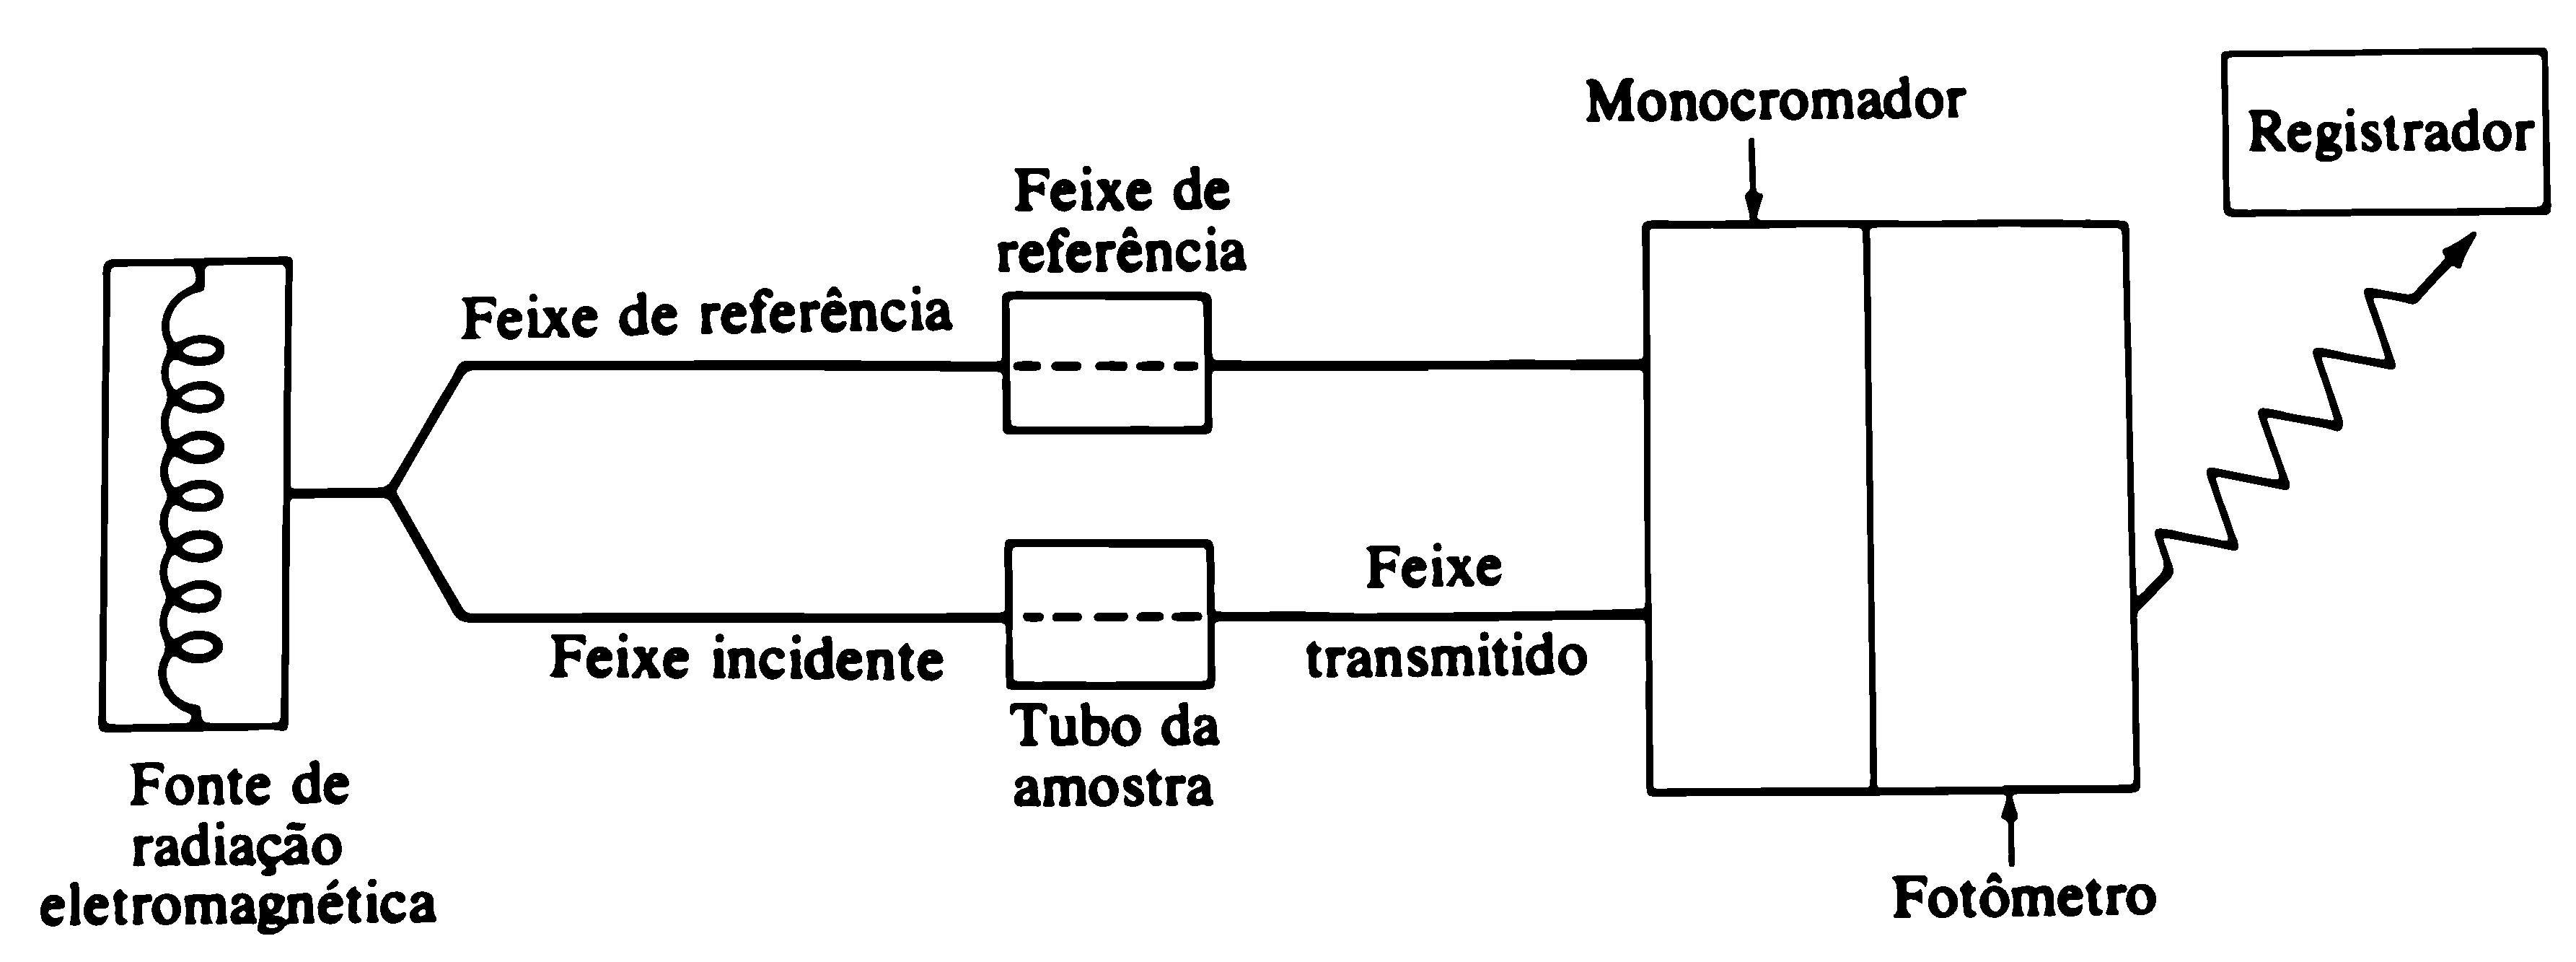
\includegraphics[width=0.9\textwidth,angle=0]{content/images/Figura_9_1.pdf}
    \caption{Diagrama esquemático de um espectrofotômetro simples.}
    \label{figura_9_1}
\end{figure}

A Figura \ref{figura_9_2} mostra o espectro do $n$-hexano no infravermelho. Note que é habitual apresentar o espectro em função da luz transmitida (de 0 a 100\%) e não em função da luz absorvida. Assim, os espectros no infravermelho mostram absorção \textit{máxima} nos \textit{mínimos} do gráfico, ao contrário dos espectros de RMN onde é habitual usar-se absorção.

\begin{figure}[H]
    \centering
    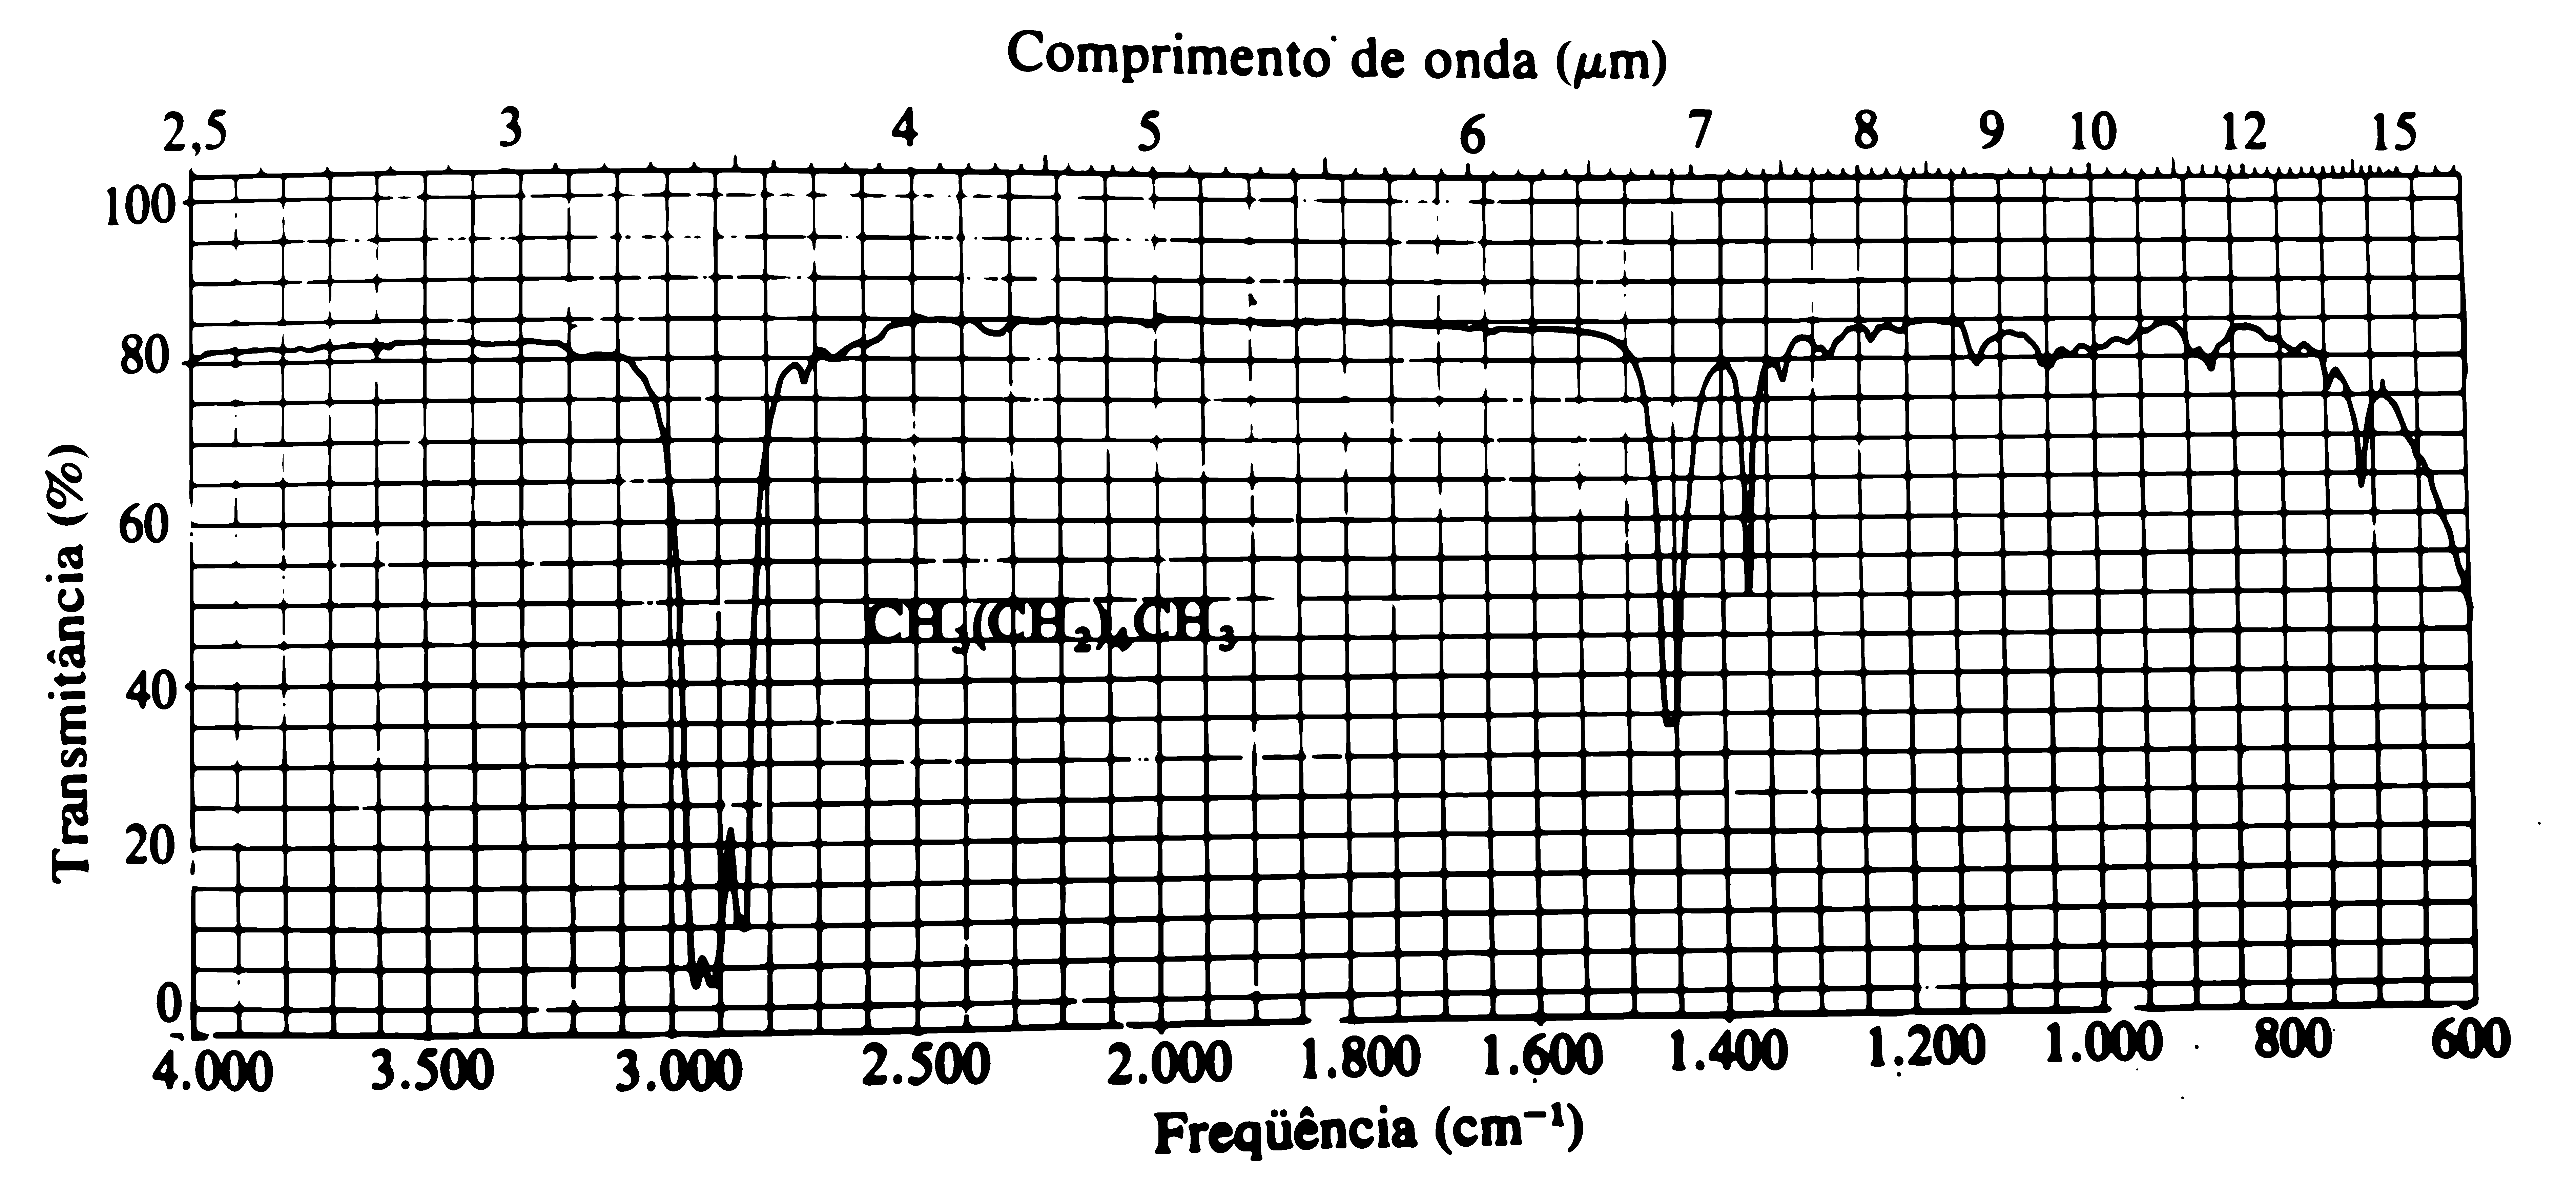
\includegraphics[width=0.9\textwidth,angle=0]{content/images/Figura_9_2.pdf}
    \caption{Espectro do $n$-hexano no infravermelho (filme líquido).}
    \label{figura_9_2}
\end{figure}

Em muitos partes do gráfico a transmitância é próxima de 100\%, significando que a substância é transparente à radiação daquelas frequências. Note as fortes bandas de absorção a 2900 a 1450 cm$^{-1}$, que resultam dos movimentos de deformação axial e angular da ligação \ch{C-H}, respectivamente. As bandas de absorção não são linhas finas porque os níveis de energia vibracional têm a eles associados um certo número de níveis rotacionais e as transições entre estes níveis causam o alargamento das bandas.

O espectro de substâncias no infravermelho pode ser obtido nos estados \textit{líquido} (líquidos homogêneos não contendo solventes), no gasoso ou sólido ou, ainda, em solução. No caso de espectros de soluções um tubo contendo \textit{apenas} o \textit{solvente} pode ser colocado no feixe de referencia (Figura \ref{figura_9_1}). A absorção do solvente no feixe incidente é compensada pela absorção no feixe referência e obtém-se assim o registro apenas do soluto.

A energia absorvida na excitação de uma molécula a um estado de energia mais alto é liberada quando a molécula retorna a um estado de energia mais baixo. Na região do infravermelho a energia é liberada sob a forma de calor, o que causa um aumento temperatura da amostra.

Diferentes tipos de átomos têm diferentes massas. Diferentes tipos de ligações têm forças de ligação diferentes, as quais aproximadamente independentes dos átomos que não participam diretamente da ligação sob exame (exceto no caso de sistemas conjugados e outros casos especiais). Logo, combinações diferentes de masses atômicas e energias de ligação dão origem a sistemas que vibram a frequências diferentes quando a molécula absorve energia eletromagnético. Por exemplo, o sistema de ligações, \ch{O-C-O} do dióxido de carbono absorve energia de número de ondas 667 cm$^{-1}$ quando há deformação angular, enquanto no sistema \ch{H-O-H} o mesmo acontece a 1595 cm$^{-1}$.

\begin{figure}[H]
    \centering
    \chemnameinit{}
    \chemname[0.8ex]{\chemname[2ex]{\chemfig[][scale=0.7]{\chemabove{O}{\footnotesize\uparrow}=\chembelow{C}{\footnotesize\downarrow}=\chemabove{O}{\footnotesize\uparrow}}}{\footnotesize{Deformação angular de \ch{O-C-O}}}}{\footnotesize{$n$ = 667 cm$^{-1}$}}
    \chemnameinit{}
    \qquad\qquad\qquad\qquad
    \chemname[0.8ex]{\chemname{\chemfig[][scale=0.7]{\chemabove{H}{\footnotesize\nwarrow}(-[1]\chembelow{O}{\footnotesize\downarrow}(-[7]\chemabove{H}{\footnotesize\nearrow}))}}{\footnotesize{Deformação angular de \ch{H-O-H}}}}{\footnotesize{$n$ = 1595 cm$^{-1}$}}
    \chemnameinit{}
\end{figure}

Os diferentes movimentos vibracionais dos átomos de uma molécula podem levar também à absorção em diferentes números de onda. Considere, por exemplo, a molécula da água. Os movimentos dos dois hidrogênios não são independentes, havendo um acoplamento entre eles, como acontece com dois pêndulos com suas origens na mesma barra. Este acoplamento leva a um movimento simétrico, no qual os dois hidrogênios se afastam e se aproximam ao mesmo tempo, e a um movimento assimétrico, no qual um dois hidrogênios se aproxima do oxigênio enquanto o outro se afasta. Uma ligação \ch{O-H} isolada, isto é, sem os efeitos do acoplamento, teria uma vibração de deformação axial absorvendo a 3700 cm$^{-1}$ (equidistante das vibrações simétrica e assimétrica). A mudança em qualquer um desses movimentos requer absorção de diferentes quantidades de energia, o que leva à absorção em frequências características do espectro no infravermelho. Assim, a molécula \ch{H2O} tem um total de três absorções características a frequências diferentes:

\begin{figure}[H]
    \centering
    \chemnameinit{}
    \chemname[0.8ex]{\chemname[2.5ex]{\chemfig[][scale=0.7]{\chembelow{H}{\footnotesize{\swarrow}}(-[1]O(-[7]\chembelow{H}{\searrow}))}}{\footnotesize{Deformação axial simétrica}}}{\footnotesize{$n$ = 3655 cm$^{-1}$}}
    \chemnameinit{}
    \qquad\qquad\qquad\qquad
    \chemname[0.8ex]{\chemname[2.5ex]{\chemfig[][scale=0.7]{\chembelow{H}{\footnotesize{\swarrow}}(-[1]O(-[7]\chembelow{H}{\nwarrow}))}}{\footnotesize{Deformação axial assimétrica}}}{\footnotesize{$n$ = 3756 cm$^{-1}$}}
    \chemnameinit{}
    \qquad\qquad\qquad\qquad
    \chemname[0.8ex]{\chemname[2.5ex]{\chemfig[][scale=0.7]{\chemabove{H}{\footnotesize{\nwarrow}}(-[1]O(-[7]\chemabove{H}{\nearrow}))}}{\footnotesize{Deformação angular}}}{\footnotesize{$n$ = 1595 cm$^{-1}$}}
    \chemnameinit{}
\end{figure}

\noindent\textbf{Espectro de hidrocarbonetos no infravermelho}

O acoplamento de frequências vibracionais ocorre mais efetivamente quando as frequências são próximas. Nas moléculas orgânicas há usualmente muitas ligações \ch{C-C} e \ch{C-H} e as frequências de vibração dos átomos geralmente se acoplam dando um espectro muito complicado. Entretanto, certas características são identificáveis nos espectros dos hidrocarbonetos. No espectro do $n$-hexano (Figura \ref{figura_9_2}), as bandas de absorção mais fortes são observadas a 2900 e 1450 cm$^{-1}$, originando-se nas deformações axial e angular, respectivamente. Todos as moléculas que contêm grupos alquila mostram essas bandas de absorção que são, portanto, encontradas em quase todos os espectros de compostos orgânicos no infravermelho. A deformação angular simétrica de um a grupamento metila leva à absorção a aproximadamente 1380 cm$^{-1}$. O grupamento metila terminal de grupamentos alquila mostra esta absorção e consequentemente uma banda a 1380 cm$^{-1}$ é encontrada na maioria dos espectros de compostos orgânicos.

A ligação \ch{C+C} é mais forte do que ligação \ch{C=C} e em consequência a deformação axial é mais difícil. A formação axial da ligação \ch{C+C} é responsável, portanto, pela absorção a um número de ondas mais alto do que a deformação axial da ligação \ch{C=C}. Esta última, por outro lado, causa absorção a um número de onda mais alto do que a deformação axial ligação \ch{C-C}. Graças ao acoplamento dos modos de vibração de deformação axial das ligações \ch{C-C} e \ch{C-H}, a região 1.400-800 cm$^{-1}$ do espectro de uma molécula tipica é usualmente muito complicada e as bandas não podem ser individualmente associadas a determinadas ligações. Por outro lado, esta região é característica de uma determinada molécula. Esta parte do espectro é conhecido como a região da impressão digital, por razões óbvias.

\noindent MATÉRIA OPCIONAL
Relações entre as frequências vibracionais e as propriedades de ligação. Em uma aproximação grosseira todas as ligações simples têm forças de ligação ou constantes de força de deformação axial semelhantes e a energia para esta deformação é dada por:

\begin{equation}
    E = \dfrac{1}{2}k(\delta l )^2
\end{equation}

A constante $K$ é chamada a constante de força e mede a resistência de ligação ao movimento de deformação axial. A quantidade $\delta l$ é uma medida da extensão da deformação. Este tipo de relação é o mesmo que descreve classicamente o movimento de duas massas ligadas por molas (lei do Hooke).

Para ligações duplas, \ch{X=Y}, as constantes de força são mais ou menos o dobro das observadas para ligações simples e para ligações triplas, \ch{X+Y}, o triplo. A frequência vibracional da ligação \ch{X-Y} em cm$^{-1}$, quando a massa de Y é muito maior do que a da X, é dada por:

\begin{equation}
    v = \dfrac{1}{2 \pi c}\sqrt{\dfrac{k}{m_x}}
\end{equation}

\noindent onde $k$ é a constante de força para a deformação axial, $m_x$ é massa do átomo X, e $c$ é a velocidade da luz. Para X constante as razões das frequências de vibração de \ch{X-Y}, \ch{X=Y} e \ch{X+Y} são aproximadamente 1, $\sqrt{2}$ e $\sqrt{3}$. Note, também, que quando $m_x$ aumenta a frequência diminui, porque neste caso é proporcional a $\dfrac{1}{\sqrt{m_x}}$. Como a massa do hidrogênio é pequena, as frequências de vibração de deformação axial da ligações \ch{H-Y} são excepcionalmente altas.

Podemos agora construir o diagrama sumariando as regiões de absorção no infravermelho de ligações carbono-carbono e carbono-hidrogênio (Figura 9.3). A absorção de deformação axial de \ch{C-H} ocorre próxima a 2900 cm$^{-1}$ (alquila), 3100 cm$^{-1}$ (vinila) e 3300 cm$^{-1}$ (\ch{H-C+C\bond{normal}}).

\begin{figure}[H]
    \centering
    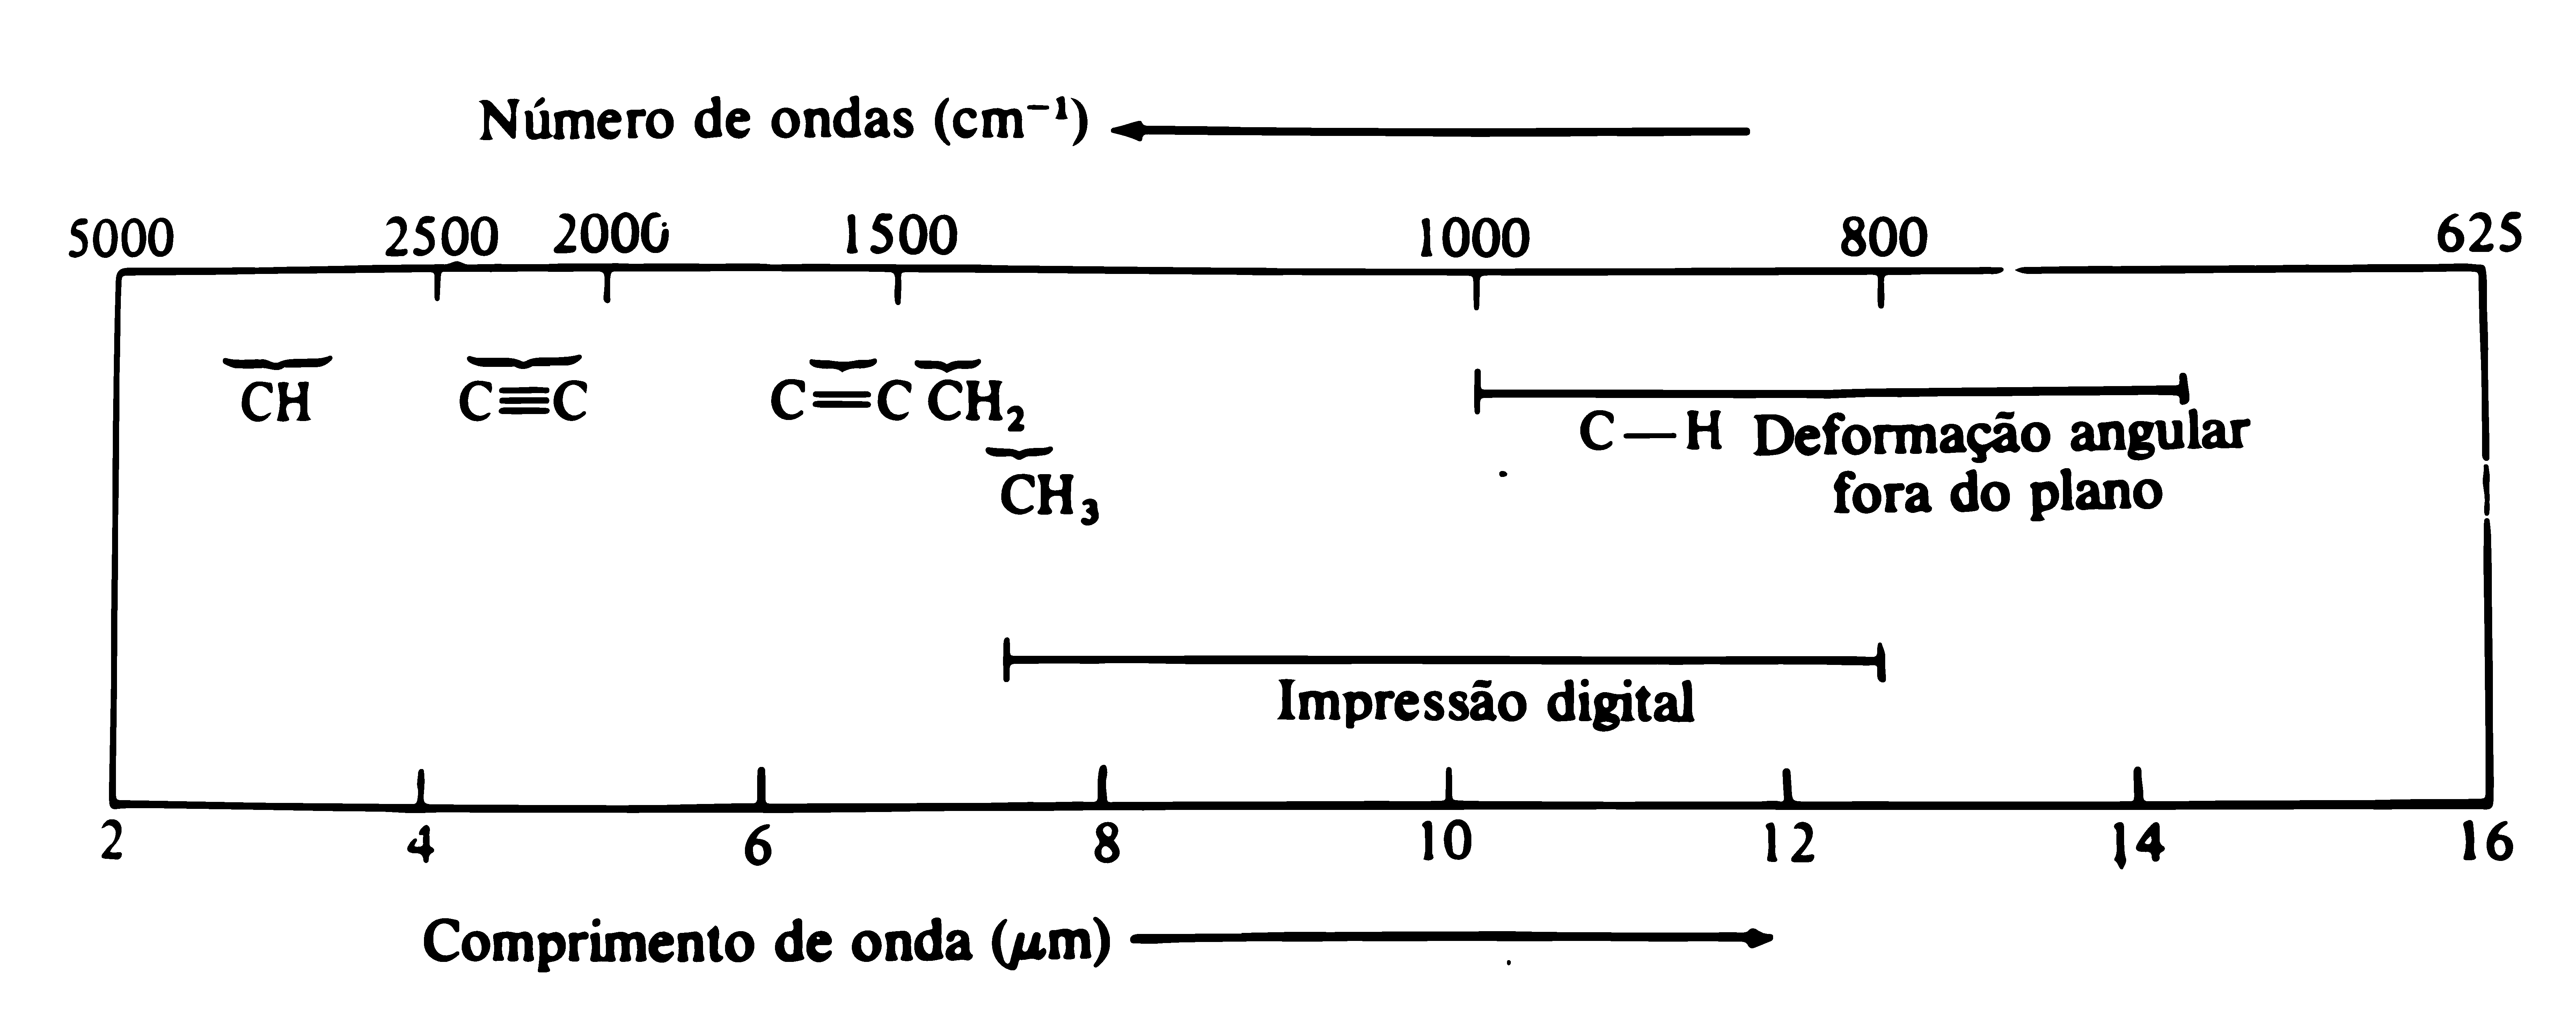
\includegraphics[width=0.9\textwidth,angle=0]{content/images/Figura_9_3.pdf}
    \caption{Regiões de absorção de ligações \ch{C-C} e \ch{C-H} no infravermelho.}
    \label{figura_9.3}
\end{figure}

Ligações triplas absorvem a 2300-2100 cm$^{-1}$ e ligações duplas próximas a 1650 cm$^{-1}$. Hidrogênios vinílicos mostram bandas fortes correspondendo às 'deformações angulares fora do plano' na região 1000-700 cm$^{-1}$. Muitas destas características aparecem no espectro do metileno-ciclo-hexano (Figura \ref{figura_9_4}).

\noindent\textbf{Espectro IV de grupos funcionais}

\noindent Os espectros de infravermelho são regularmente usados pelos químicos orgânicos para facilitar a identificação de grupos funcionais. Comparando os espectros das Figuras \ref{figura_9_4}-\ref{figura_9_7} vemos como a presença e a ausência de absorções específicas podem ser usadas para reconhecer-se a presença ou a ausência de determinado grupo funcional em uma molécula.

O espectro no infravermelho do 1-hexanol (Figura \ref{figura_9_5}) ilustra a absorção de deformação axial característica da hidroxila de um álcool em ligação hidrogênio - a banda larga e forte a 3330 cm$^{-1}$ e mostra também a absorção da ligação \ch{C-O} a 1060 cm$^{-1}$. Em contraste, o espectro do dietil-éter (Figura 9.6) não apresenta a absorção da hidroxila a 3330 cm$^{-1}$ mas tem uma absorção forte a 1125 cm$^{-1}$, característica da deformação axial da ligação \ch{C-O}.

O espectro do butirato de etila no infravermelho (Figura \ref{figura_9_7}) mostra absorção forte na região de 1730 cm$^{-1}$ atribuída à vibração de deformação axial da carbonila. A Figura \ref{figura_9_7} não mostra, por outro lado, a banda característica da deformação axial de \ch{O-H} de álcoois em ligação hidrogênio a 3330 cm$^{-1}$ (Figura \ref{figura_9_5}), mas tem a deformação axial de \ch{C-O} a 1180 cm$^{-1}$ (Figura \ref{figura_9_6}). As Figuras \ref{figura_9_4}-\ref{figura_9_6} não mostram a absorção forte a 1.730 cm$^{-1}$ característica de \ch{C=O} (Figura \ref{figura_9_7}). Podemos concluir que o composto da Figura \ref{figura_9_7} contém um grupo carbonila, o que não acontece com os das Figuras \ref{figura_9_4}-\ref{figura_9_6}, que a Figura \ref{figura_9_4} corresponde a um composto não contém nenhum dos grupos funcionais que aparecem nas Figuras 9.5-9.7, e que todos os compostos das Figuras \ref{figura_9_5}-\ref{figura_9_7} contêm ligações \ch{C-O}. Deste modo, os químicos podem comparar os espectros de compostos conhecidos com espectros de compostos desconhecidos e, frequentemente, identificar os grupos funcionais presentes nos desconhecidos.

\begin{figure}[H]
    \centering
    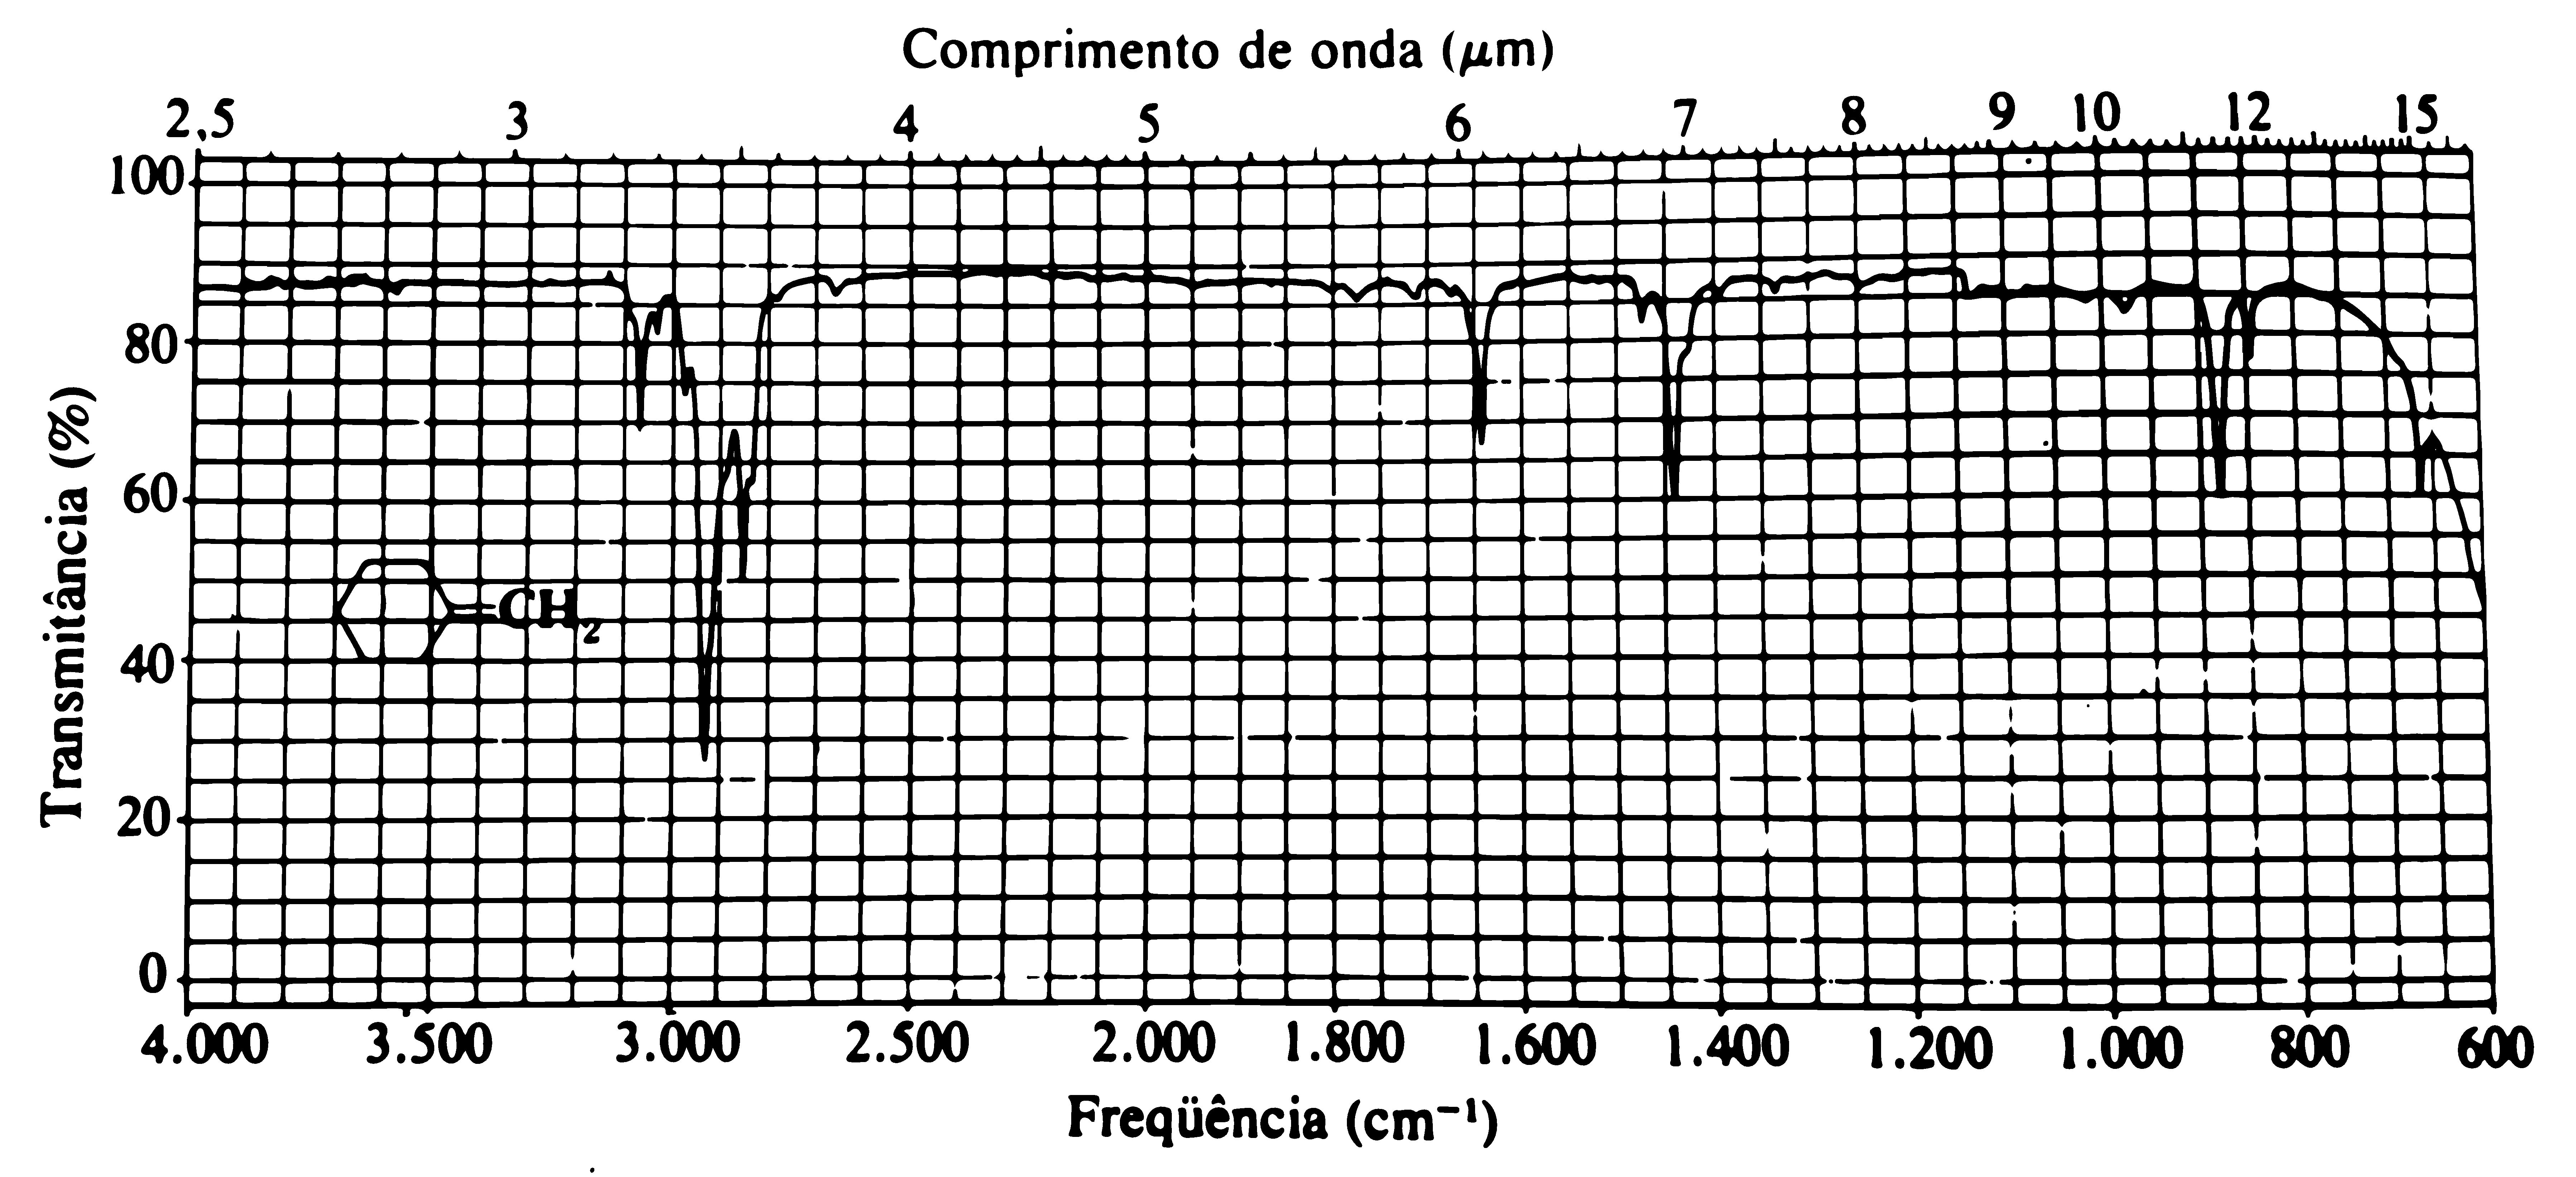
\includegraphics[width=0.85\textwidth,angle=0]{content/images/Figura_9_4.pdf}
    \caption{Espectro do metileno-ciclo-hexano no infravermelho (filme líquido).}
    \label{figura_9_4}
\end{figure}

\begin{figure}[H]
    \centering
    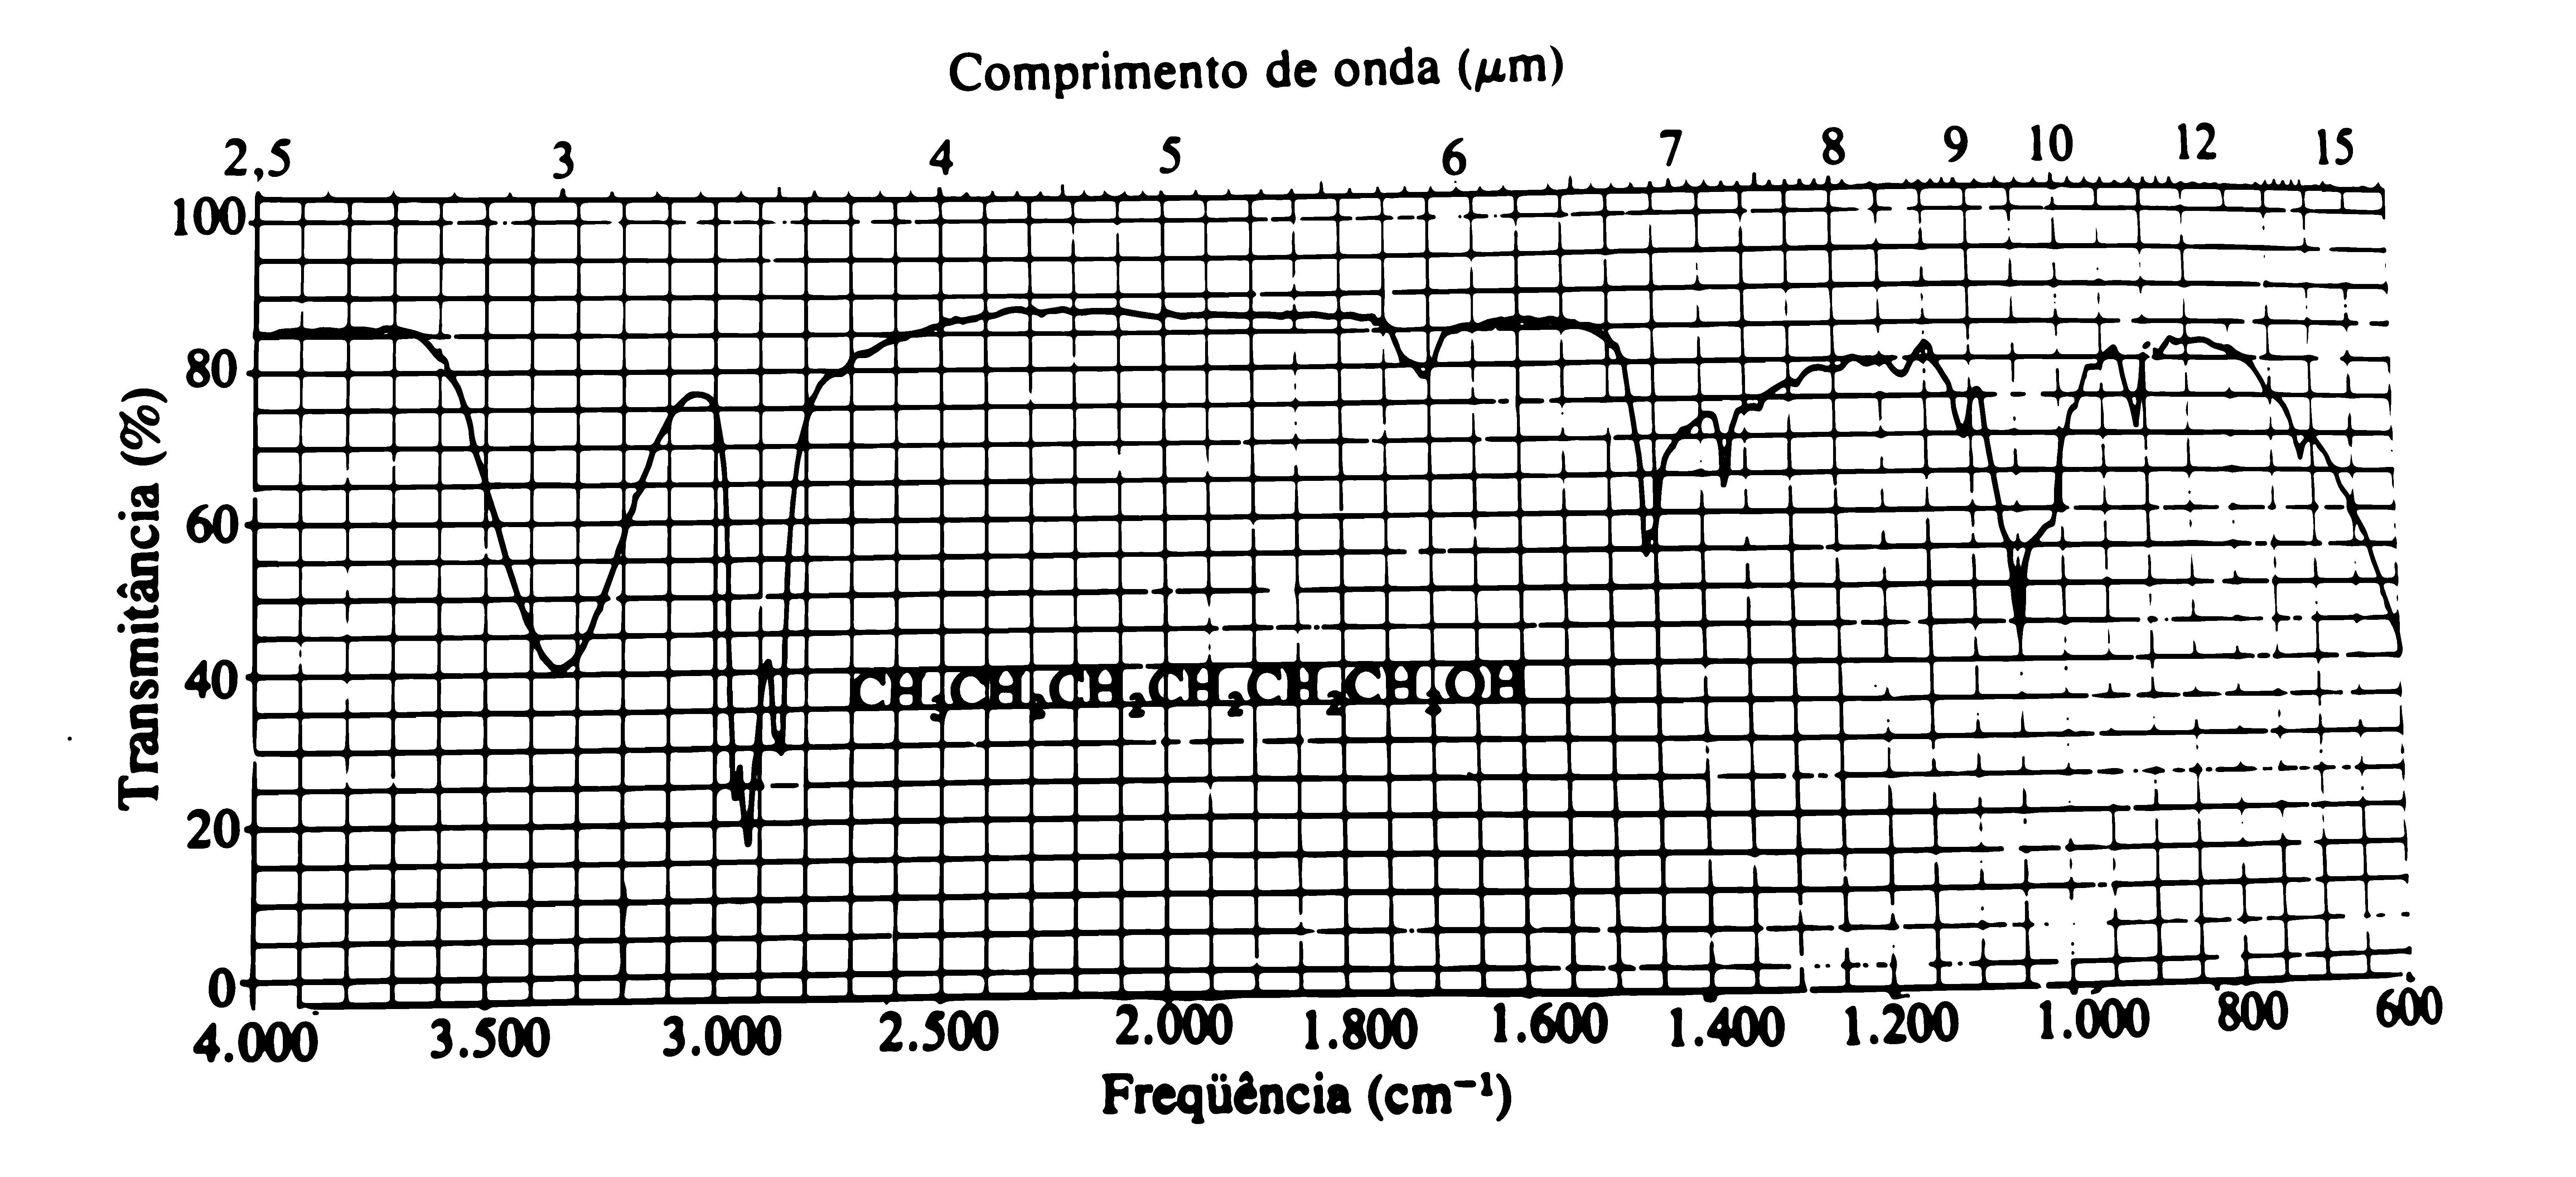
\includegraphics[width=0.9\textwidth,angle=0]{content/images/Figura_9_5.pdf}
    \caption{Espectro do 1-hexanol no infravermelho (filme líquido).}
    \label{figura_9_5}
\end{figure}

\begin{figure}[H]
    \centering
    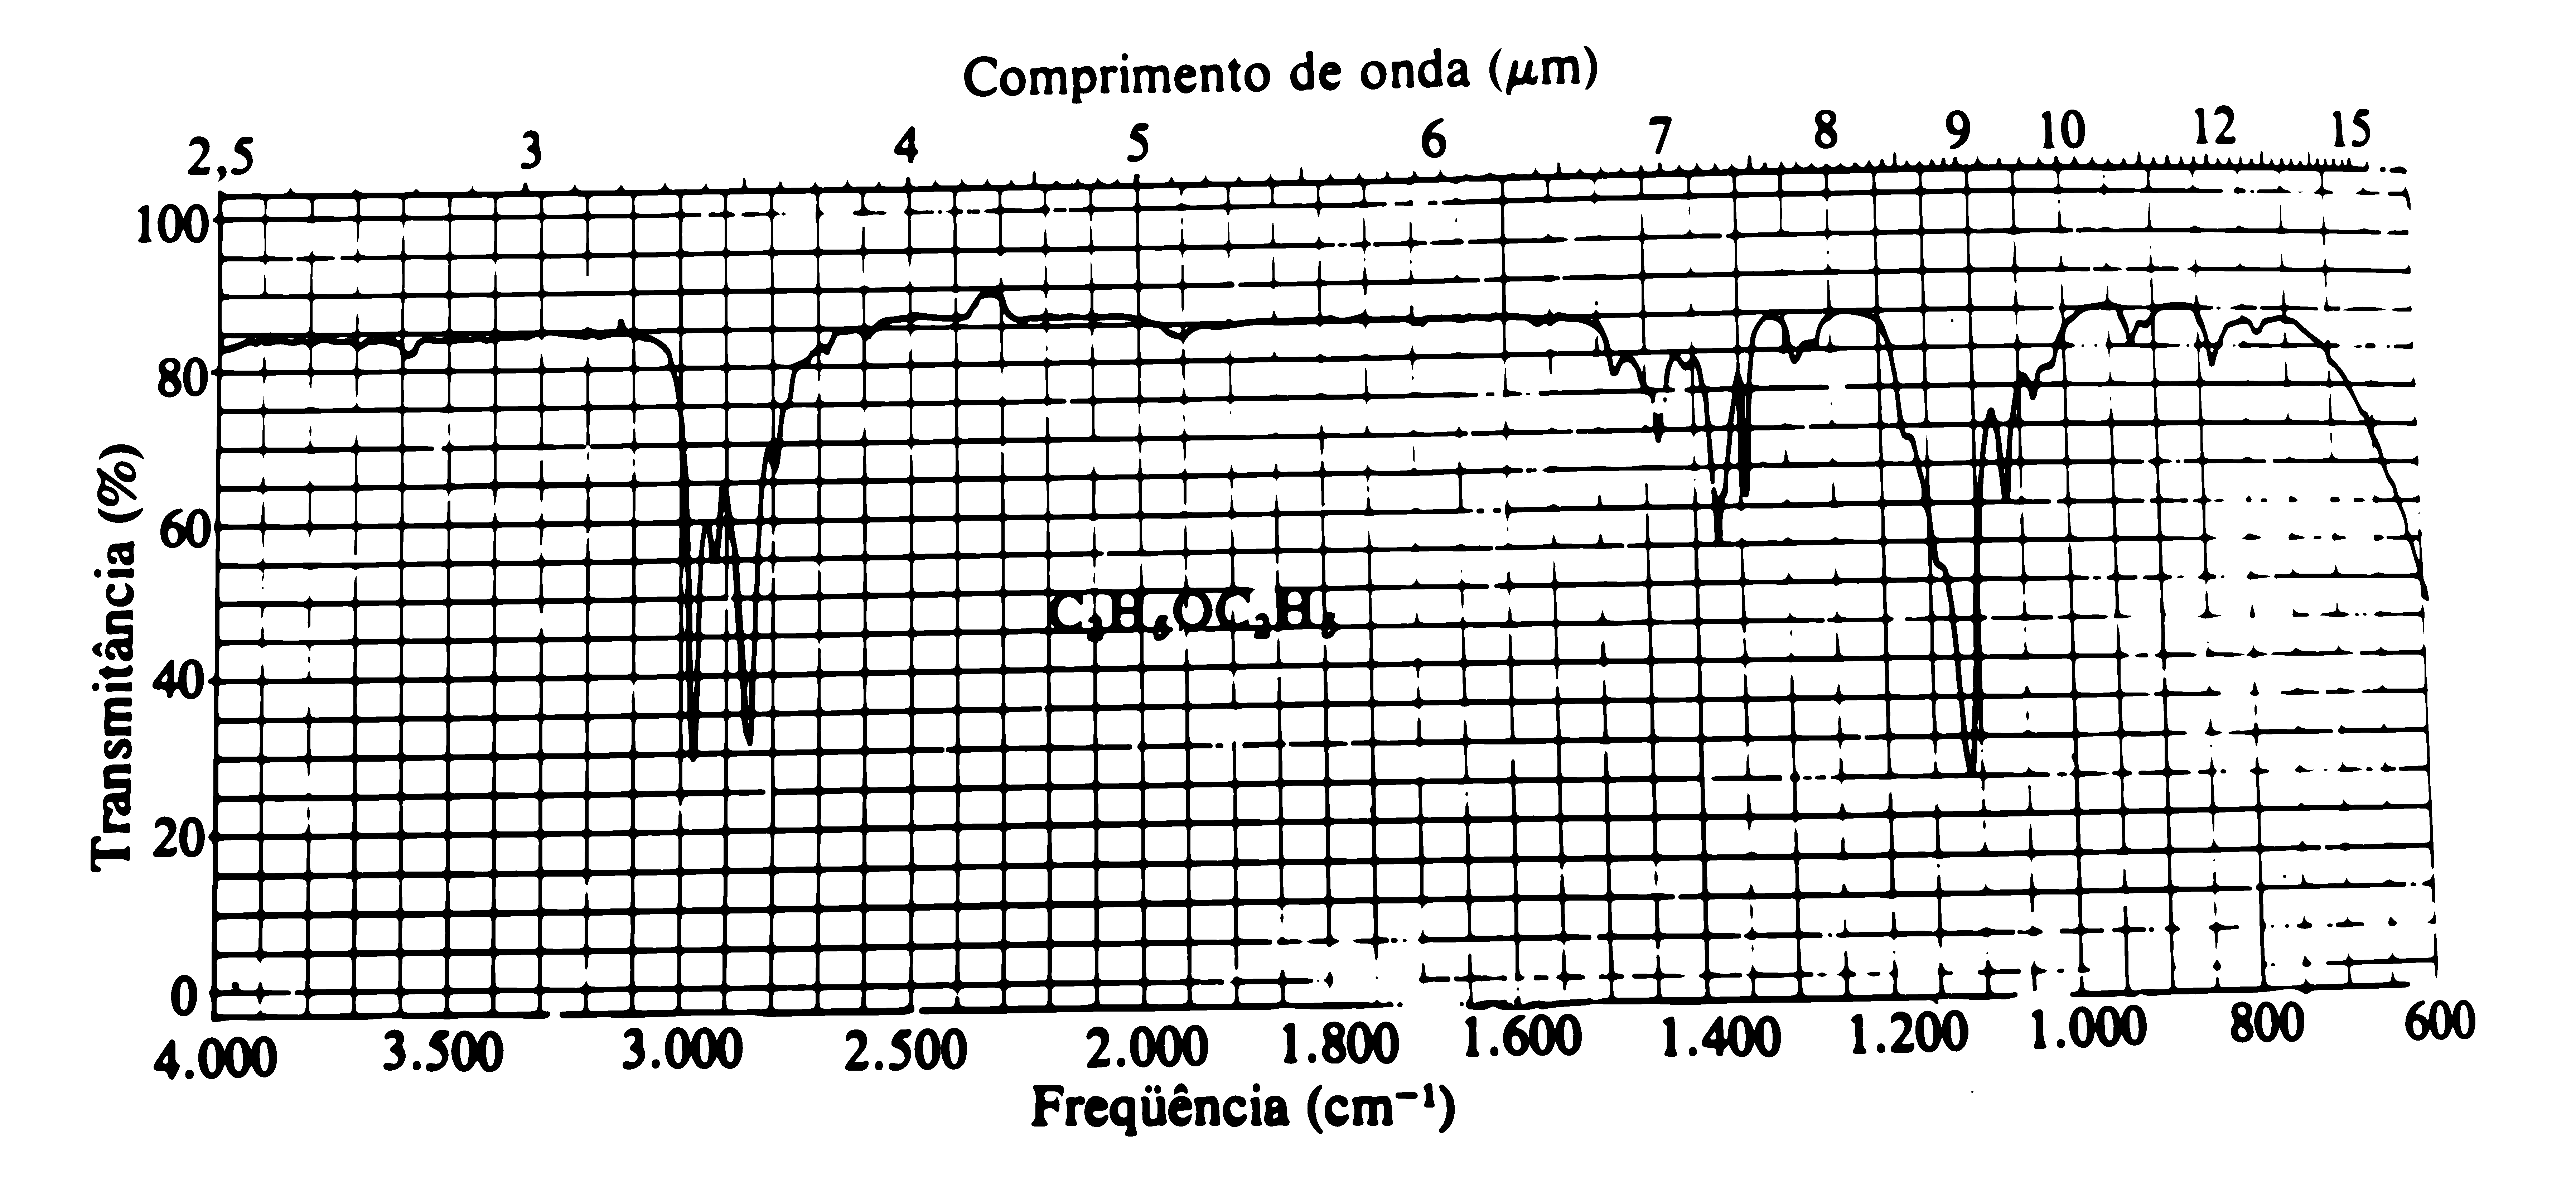
\includegraphics[width=0.9\textwidth,angle=0]{content/images/Figura_9_6.pdf}
    \caption{Espectro do dietil-éter no infravermelho (filme líquido).}
    \label{figura_9_6}
\end{figure}

\begin{figure}[H]
    \centering
    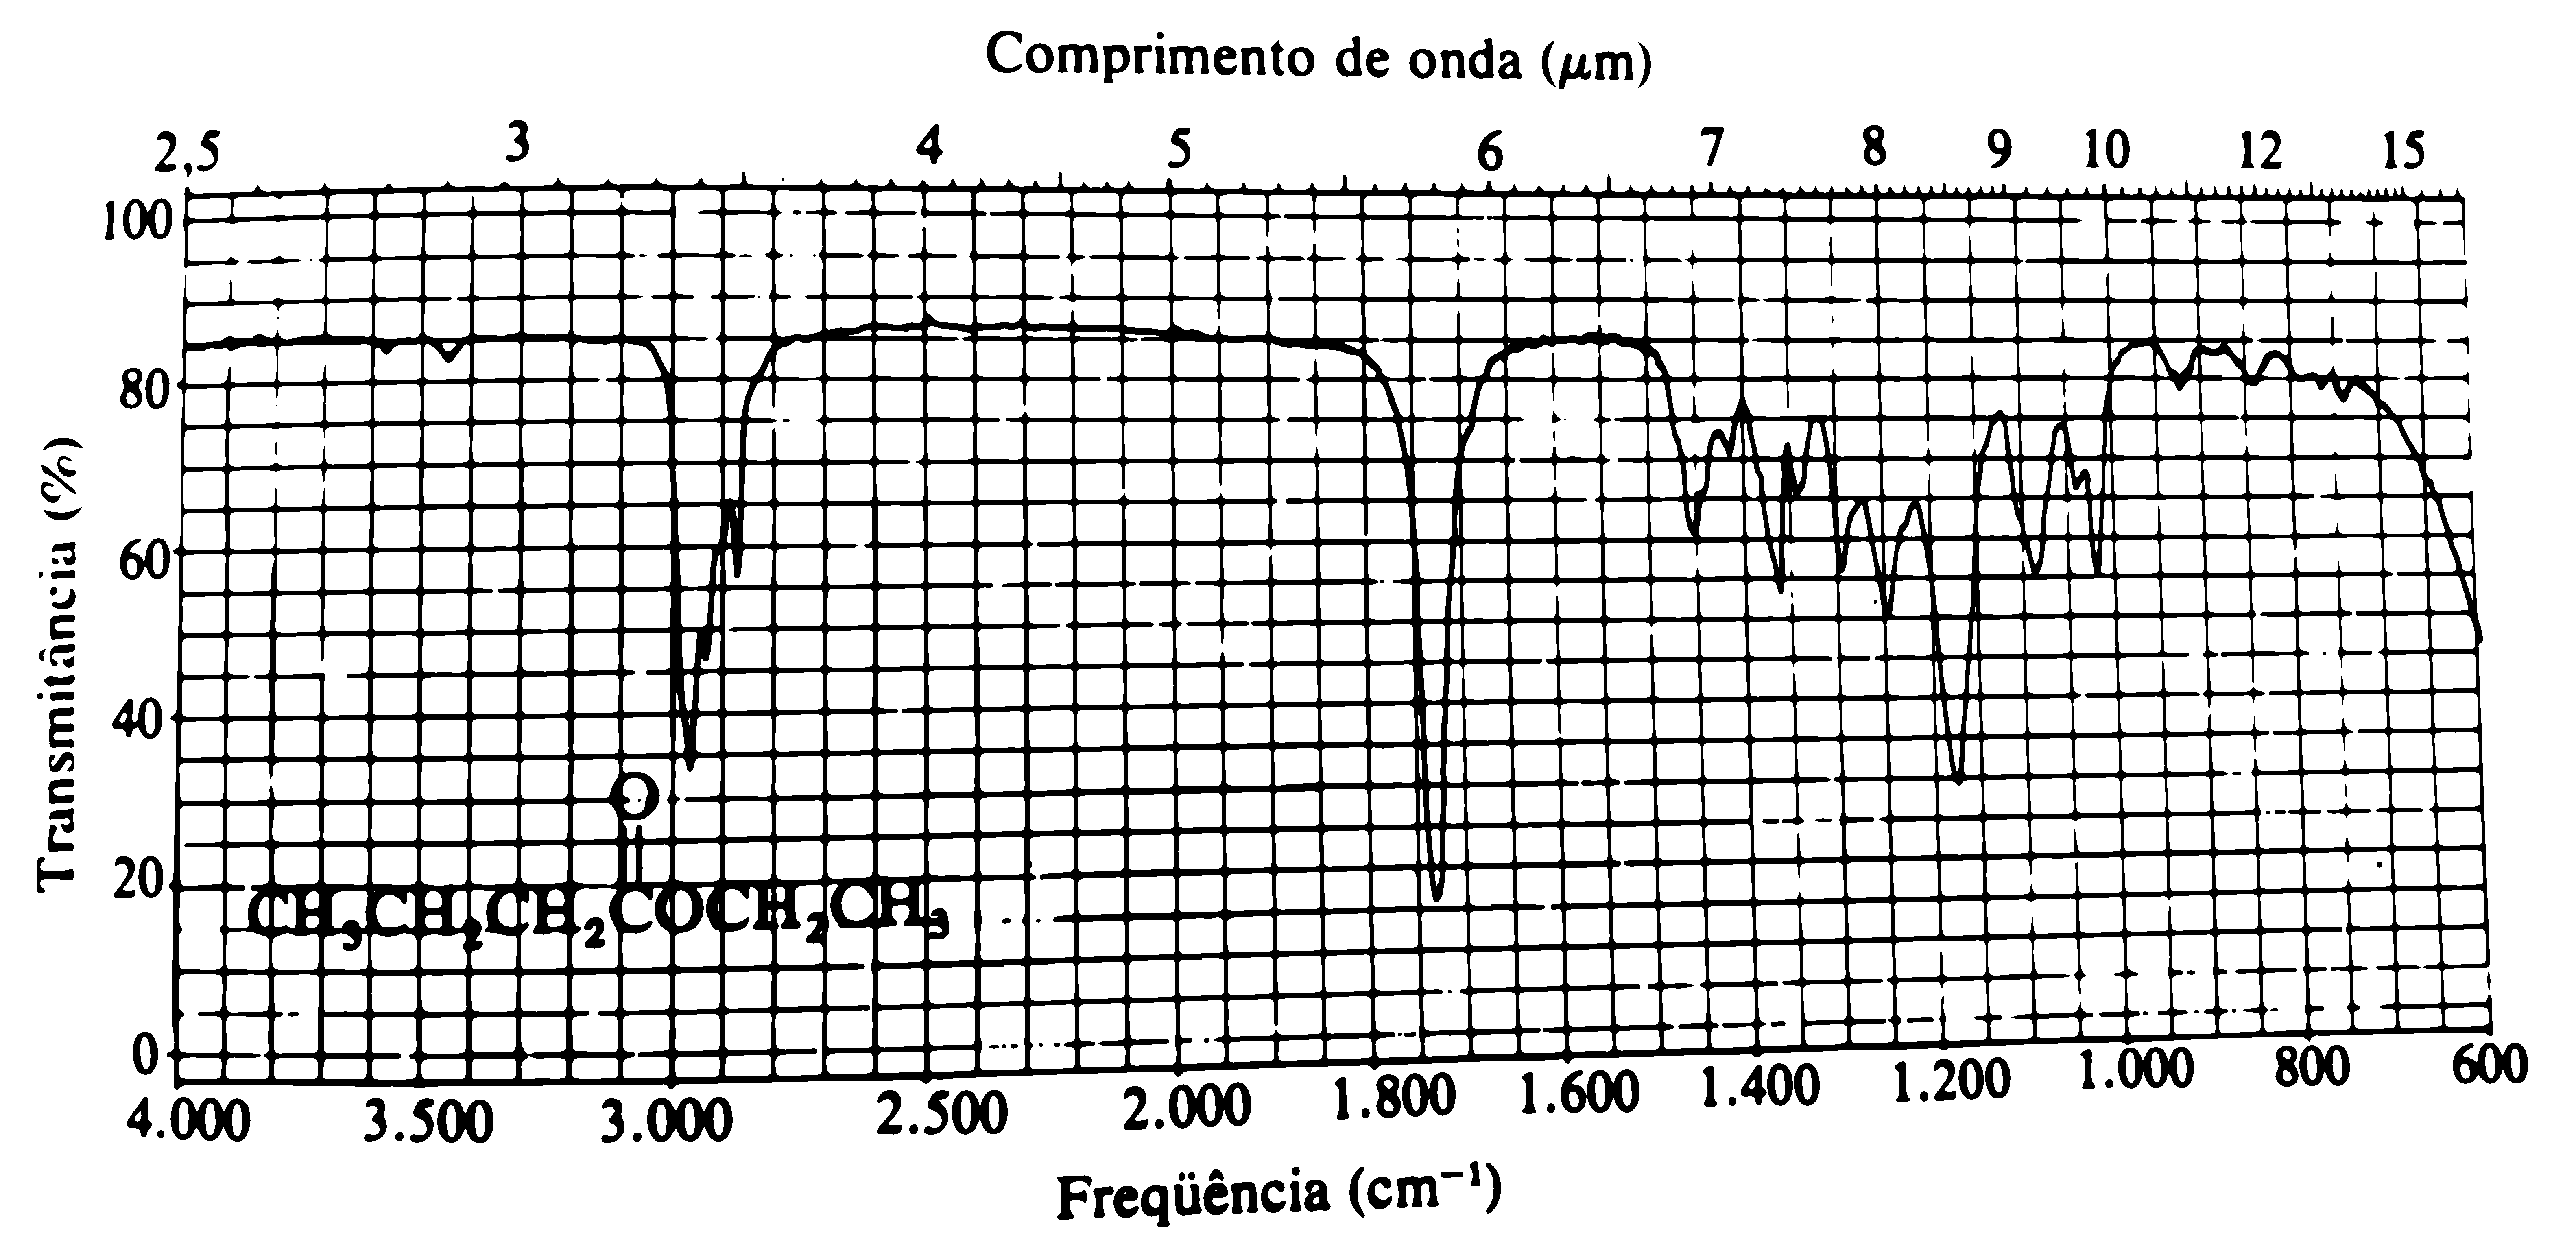
\includegraphics[width=0.9\textwidth,angle=0]{content/images/Figura_9_7.pdf}
    \caption{Espectro do butirato no infravermelho (filme líquido).}
    \label{figura_9_7}
\end{figure}

Nos espectros de RMN a intensidade do pico é proporcional ao número de prótons que contribuem para aquele pico. Nos espectros no infravermelho não existe uma relação deste tipo. A intensidade de um dado pico no infravermelho é proporcional à variação do momento de dipolo da molécula causada pela absorção. Esta variação não é previsível, em geral, em uma forma simples, entretanto algumas generalizações feitas podem ser úteis.

Primeiro, a vibração de uma ligação polar (\ch{C-O}, \ch{C=O}, \ch{C-Br}) deve levar a uma variação maior do momento de dipolo da molécula do que a de uma ligação menos polar (\ch{C-C}, \ch{C-N}, \ch{C=N}) e, portanto, os grupos mais polares levam, geralmente, a bandas de absorção mais fortes. Segundo, a vibração através de um centro de simetria não causa mudança no momento de dipolo e tais vibrações levam a absorções muito fracas (ou a nenhuma absorção) no infravermelho. Assim, a absorção de deformação axial a cerca de 1.650 cm$^{-1}$ é muito fraca no etileno e no tetrametil-etileno mas é mais forte no propano e no isobutileno.

Em geral os sistemas conjugados absorvem a frequência mais baixas do que os sistemas não conjugados. Por exemplo, os alquenos absorvem a 1670-1640 cm$^{-1}$ enquanto que os alquenos conjugados com um grupo carbonila ou outra ligação dupla absorvem a cerca de 1.600 cm$^{-1}$. Estas variações podem ser interpretadas em termos de formas ressonantes, como no butadieno:

\begin{figure}[H]
    \centering
    \schemestart
        \chemfig[][scale=0.7]{CH_2=CH-CH=CH_2}
        \arrow{<->}
        \chemfig[][scale=0.7]{^{-}CH_2-CH=CH=CH_2^{+}}
    \schemestop
\end{figure}

\noindent contribuições das formas iônicas tendem a enfraquecer as ligações duplas e tornar mais fortes as ligações simples. Estas formas de ressonância contribuem relativamente pouco e as variações na frequências de absorção não são muito grandes.

Na prática a absorção do grupo carbonila no infravermelho é de grande importância. A absorção é forte (Por quê?) e ocorre em uma região onde usualmente não aparecem outras bandas. É, portanto, fácil de localizar e identificar. A frequência exata da absorção de \ch{C=O} depende de um certo número de variáveis bem conhecidas. Se a frequência puder ser determinada, poderemos inferir muito da estrutura do composto. Um éster absorve a frequência maior do que uma cetona que, por sua vez, absorve a maior frequência do que uma amida. Se uma cetona está em um anel a frequência de absorção é uma função do tamanho do anel. A frequência varia inversamente com o ângulo \ch{C-C-C} do grupamento carbonila. Em regra, as carbonilas em anéis de seis membros têm frequências de absorção de valor aproximadamente o mesmo que os compostos de cadeia aberta correspondentes, enquanto que a \textit{diminuição do tamanho do anel aumenta a frequência de 30 cm$^{-1}$ por cada átomo de carbono}. Esta tendência é ilustrada abaixo:

\begin{figure}[H]
    \centering
    \chemnameinit{}
    \chemname{\chemfig[][scale=0.7]{R-C(=[2]O)-R}}{\footnotesize{1715 cm$^{-1}$}}
    \qquad
    \chemnameinit{}
    \chemname{\chemfig[][scale=0.7]{*6(----(=[2]O)--)}}{\footnotesize{1715 cm$^{-1}$}}
    \qquad
    \chemnameinit{}
    \chemname{\chemfig[][scale=0.7]{*5(---(=O)--)}}{\footnotesize{1745 cm$^{-1}$}}
    \qquad
    \chemnameinit{}
    \chemname{\chemfig[][scale=0.7]{*4(--(=[1]O)--)}}{\footnotesize{1775 cm$^{-1}$}}
\end{figure}

Quando uma ligação dupla carbono-carbono está em conjugação com uma carbonila esta \textit{conjugação abaixa de 30 cm$^{-1}$ a frequência observada da carbonila}. Este efeito é ilustrado nos exemplos seguintes.

\begin{figure}[H]
    \centering
    \chemnameinit{}
    \chemname{\chemfig[][scale=0.7]{CH_3(-[7]CH(-[5]CH_3)-CH_2-C(=[2]O)(-CH_3))}}{\footnotesize{1715 cm$^{-1}$}}
    \qquad
    \chemnameinit{}
    \chemname{\chemfig[][scale=0.7]{CH_3(-[7]C(-[5]CH_3)=CH-C(=[2]O)(-CH_3))}}{\footnotesize{1685 cm$^{-1}$}}
    \qquad
    \chemnameinit{}
    \chemname{\chemfig[][scale=0.7]{*6(---O-(=[2]O)--)}}{\footnotesize{1735 cm$^{-1}$}}
    \qquad
    \chemnameinit{}
    \chemname{\chemfig[][scale=0.7]{*6(---O-(=[2]O)-=)}}{\footnotesize{1705 cm$^{-1}$}}
\end{figure}

Vemos, então, que a frequência da carbonila no espectro no infravermelho de um composto de estrutura desconhecida pode fornecer informações úteis. Podemos saber o grupo funcional do qual a carbonila faz parte, se o grupo carbonila faz parte de uma anel ou se é conjugado.

Embora muitas bandas não possam ser relacionadas a uma vibração específica, o estudo comparativo de aproximadamente 125.000 espectros de compostos de estrutura conhecida resultou em muitas correlações empíricas que podem ser utilizadas para reconhecer-se características estruturais de compostos desconhecidos pelo exame de seus espectros no infravermelho. Na Tabela \ref{tabela_9_3} são fornecidas algumas frequências características de absorção de grupos funcionais no infravermelho. (Um quadro mais completo é dado no Apêndice).

\noindent \textbf{Comparações espectrais}

\noindent Os espectros de compostos no infravermelho contêm bandas de formas e tamanhos variados. Isto permite que um espectro no infravermelho possa ser usado como 'impressão digital' de um composto. Em caso de compostos de complexidade moderada, a \textit{superposição dos espectros de um composto desconhecido e de um composto conhecido estabelece a identidade entre os dois}. Esta comparação não é prove suficiente em dois casos especiais. Primeiro, moléculas diferentes de estrutura simples muito semelhantes, tais como pentadecano e hexadecano podem ter diferenças insignificantes e difíceis de detectar em seus espectros. Segundo, em moléculas muito grandes e complicadas, como polímeros e peptídeos, a resolução obtida no espectro é usualmente insuficiente para permitir uma identificação positiva.

\begin{table}[H]
\centering
\caption{Frequências de absorção características de grupos funcionais no infravermelho.}
\label{tabela_9_3}
    \begin{tabular*}{\textwidth}{cccc}
        \toprule
        Grupo & Classe do compostos & Frequência (cm$^{-1}$) & Intensidade \\
        \midrule
        \ch{C-H} & Alcano & 2965-2850 (deformação axial) & Forte \\
         & \ch{-CH3} & 1450 (deformação angular & Média \\
         &  & 1380 (deformação angular) & Média \\
         & \ch{-CH2-} & 1465 & Média \\
         & Alqueno & 3095-3010 (deformação axial) & Média \\
         &  & 700-1000 (deformação angular) & Forte \\
         & Alquino & \sim 3300 & Forte \\
         & Aldeído & 2900-2820 & Fraca \\
         &  & 2775-2700 & Fraca \\
        \ch{C-C} & Alcano & 700-1200 (geralmente não é útil) & Fraca \\
         & Alqueno$^a$ & 1680-1620 & Variável \\
         & Alquino$^a$ & 2260-2100 & Variável \\
        \ch{C=O}$^a$ & Cetona & 1715 & Forte \\
         & Aldeído & 1725 & Forte \\
         & Ácido carboxílico & 1710 & Forte \\
         & Ester & 1735 & Forte \\
         & Amida & 1650 & Forte \\
         & Anidrido & 1820 e 1760 & Forte \\
        \ch{C-O} & Álcool, éster, ácido carboxílico, éter & 1300-1000 & Forte \\
        \ch{O-H} & \underline{Álcool} &  &  \\
         & Monômero & 3650-3590 & Variável e aguda \\
         & Em ligação hidrogênio & 3400-3200 & Forte e larga \\
         & \underline{Ácido carboxílico} &  & \\
         & Em ligação hidrogênio & 3300-3500 & Variável e larga \\
        \ch{N-H} & Amina e amida primárias & \sim 3500 (deformação axial)$^b$ & Média \\
         & Amine e amida secundárias & 3500 (deformação axial)$^b$ & Média \\
        \ch{C+N} & Nitrila$^a$ & 2260-2240 & Média \\
        \ch{C-X} & Fluoreto & 1400-1000 & Forte \\
         & Cloreto & 800-600 & Forte \\
         & Brometo & 600-500 & Forte \\
         & Iodeto & \sim 500 & Forte \\
        \bottomrule
        \multicolumn{4}{p{0.98\textwidth}}{$^a$Não conjugada. Conjugação com ligações múltiplas abaixam de 30 cm$^{-1}$ a frequência de deformação axial.}\\
       \multicolumn{4}{p{0.98\textwidth}}{$^b$Mais baixa se em ligação hidrogênio.}
    \end{tabular*}
\end{table}

\section{INTERPRETAÇÃO DOS ESPECTROS}
Embora, não existam regras rígidas para a interpretação de um espectro no infravermelho, algumas diretrizes poder ser úteis.

\begin{enumerate}
    \item \textit{Comece pelo lado esquerdo do espectro e faça um exame preliminar da região 4000-1500 cm$^{-1}$}. Não tente interpretar com detalhes a ragião de deformação axial da ligação \ch{C-H} próxima a 3000 cm$^{-1}$. Assinale, tentativamente, todas as demais bandas. As vibrações de deformação axial características de grupos funcionais muito importantes, como \ch{OH}, \ch{NH}, \ch{C=O} e \ch{C=C}, ocorrem nesta região. Lembre-se que a ausência de absorções nas regiões habituais de vibração é muito importante para reduzir o número de compostos que deveremos considerar a seguir.
    \item \textit{Sempre que possível, o assinalamento de bandas feito acima deve ser confirmado pelo exame de outras porções do espectro.}
    \item \textit{Examine a região de deformação axial do \ch{CH} logo acima de 3000 cm$^{-1}$ para determinar se o hidrogênio está ligado a carbono insaturado.} Se tal indicação é encontrada, tente descobrir o tipo de insaturação em outras regiões do espectro.
    \item \textit{Examine o espectro na região 1500-600 cm$^{-1}$ para um a indicação de outros grupos funcionais, tais como éteres ou halogênios.} Este é um passo importante se o item 1 não revelou a presença dos grupos funcionais mais óbvios.
\end{enumerate}

\begin{figure}[H]
    \centering
    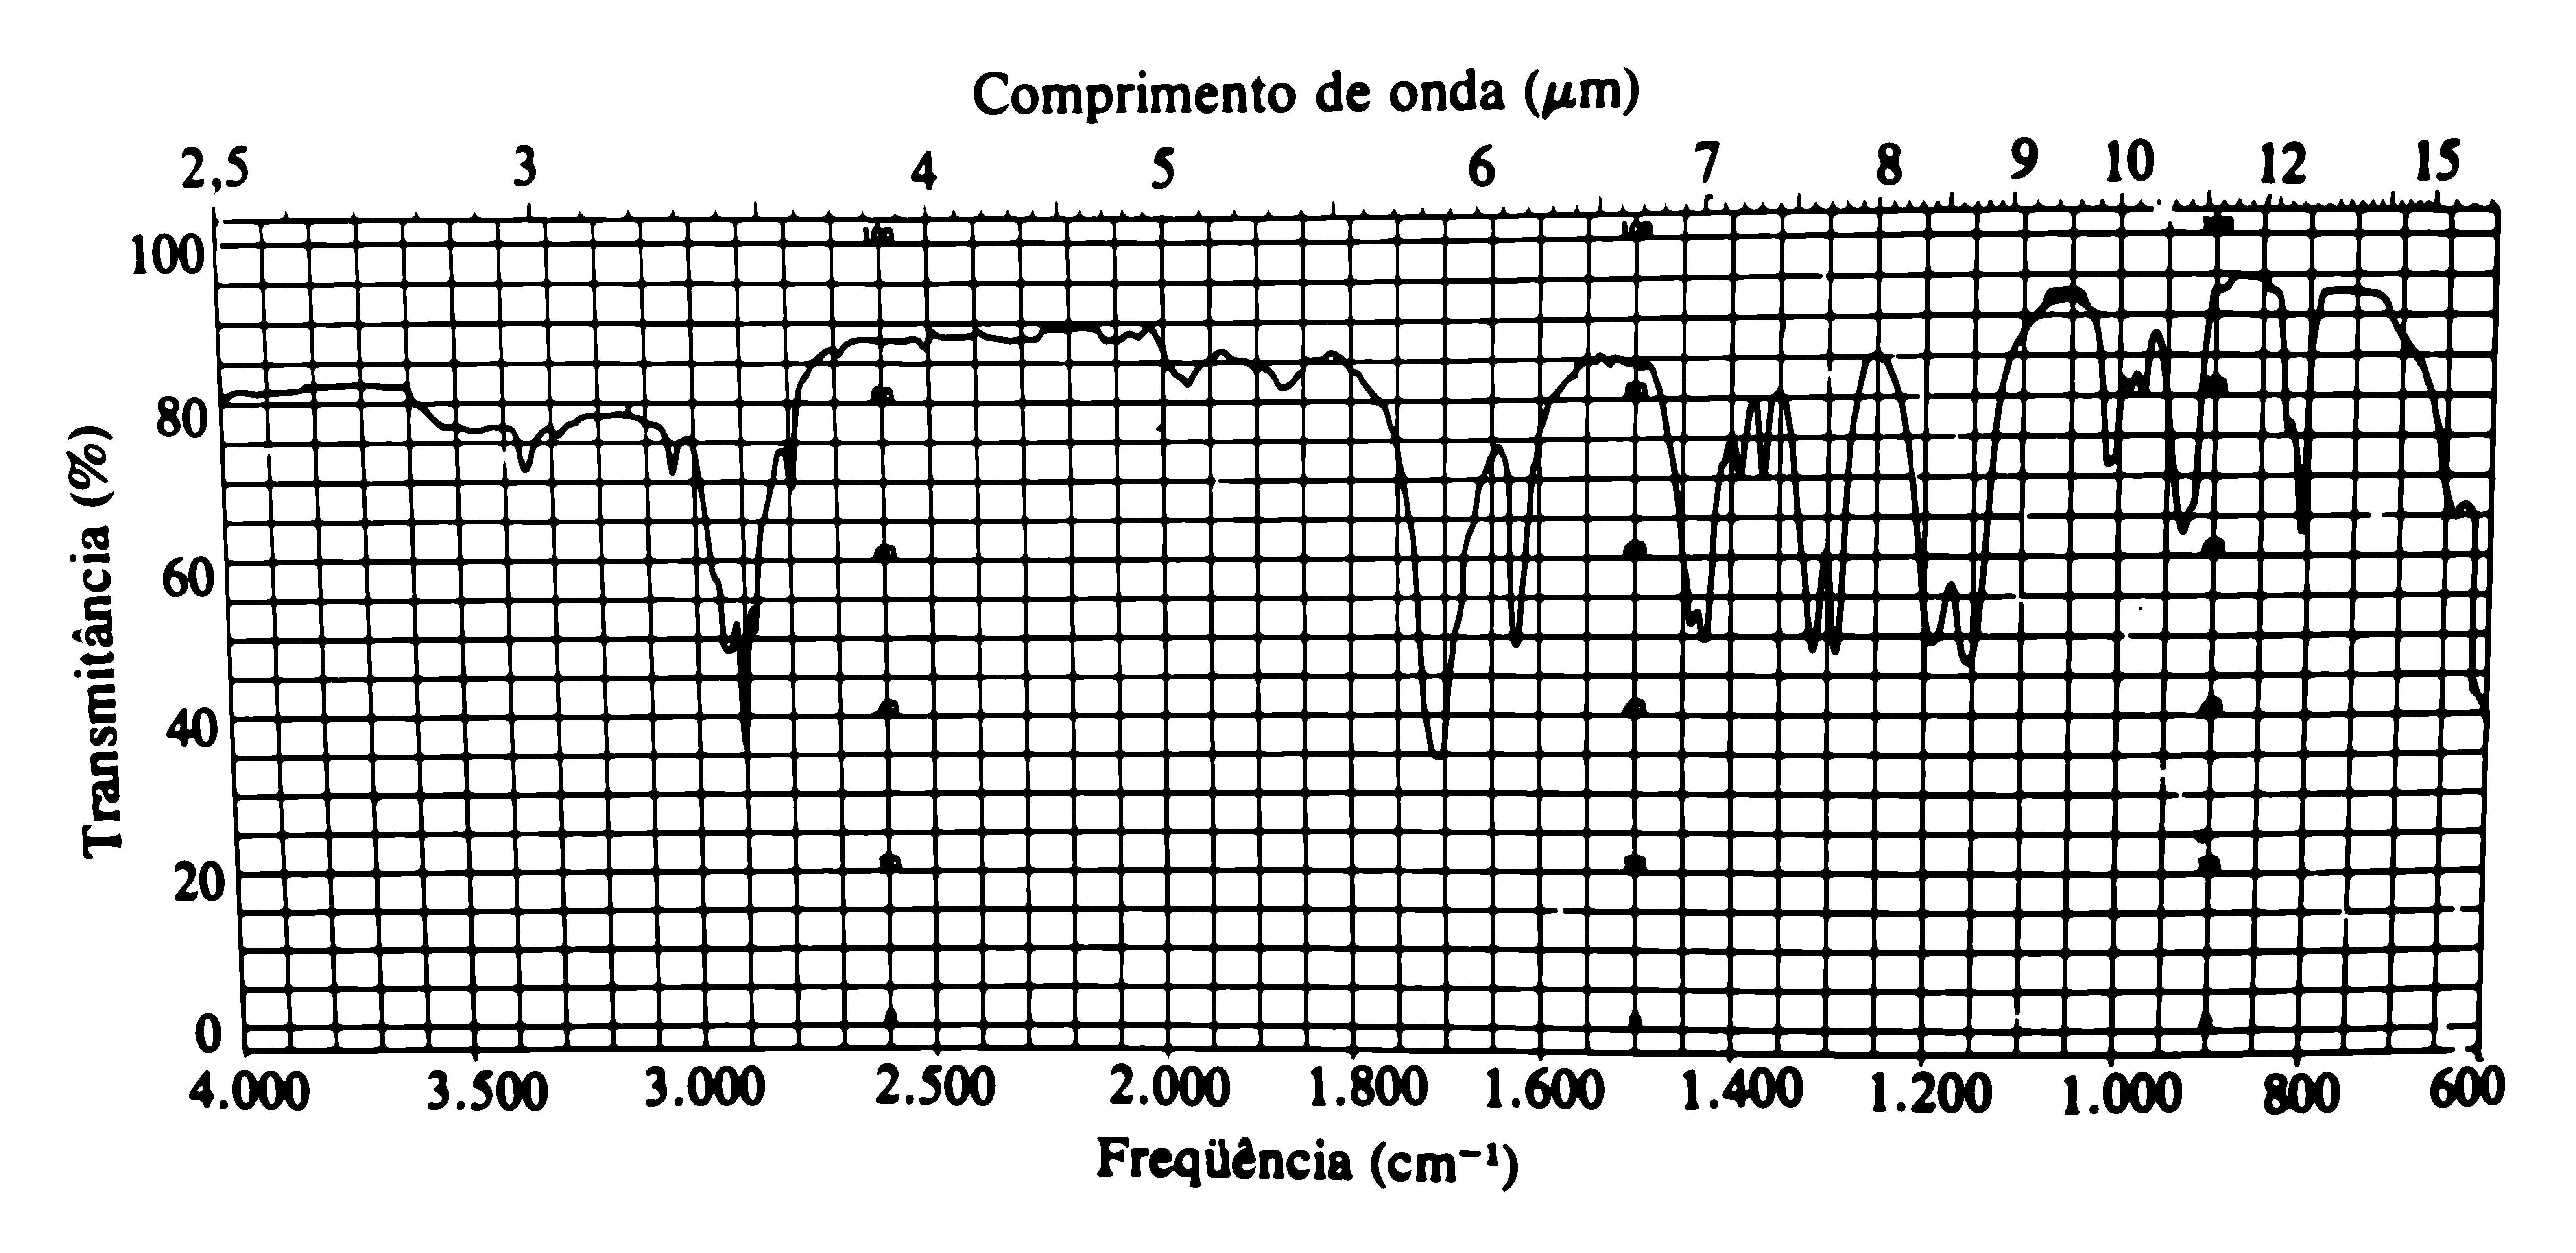
\includegraphics[width=0.9\textwidth,angle=0]{content/images/Figura_9_8.pdf}
    \caption{Espectro no infravermelho de um composto desconhecido (filme líquido).}
    \label{figura_9_8}
\end{figure}

Como um exemplo da aplicação dessa diretrizes consideremos o exemplo do espectro no infravermelho de um composto desconhecido apresentado na Figura \ref{figura_9_8}. Aplicação do item 1 revela uma banda de \ch{C=O} a 1708 cm$^{-1}$ a de \ch{C=C} a 1625 cm$^{-1}$. A banda de \ch{C=O} a 1708 cm$^{-1}$ é consistente  com a estrutura de um aldeído, cetona, ácido carboxílico ou éster. O exame de outras partes do espectro (item 2) nos permitirá a descoberta do tipo da carbonila. Um aldeído pode ser confirmado peloa presença de uma banda, ou melhor, um par de bandas a 2800 e 2700 cm$^{-1}$ (veja a Figura \ref{figura_9_9}). Um ácido carboxílico mostra uma banda muito larga característica de \ch{OH} a 3500-2500 cm$^{-1}$ (veja a Figura \ref{figura_9_11}) e foi eliminado pelo exame preliminar desta região que indicou a ausência de absorção de \ch{OH}. Um éter sempre exibe uma ou duas bandas fortes na região 1300-100 cm$^{-1}$ (veja a Figura \ref{figura_9_7}). Observe na Figura \ref{figura_9_8} as duas bandas fortes próximas a 1200 cm$^{-1}$, sugerindo fortemente que nosso desconhecido é um éster. A posição da carbonila do éster a 1708 cm$^{-1}$ sugere que o \ch{C=O} é conjugado. Olhando o espectro novamente (item 3) encontramos evidencia adicional na região do \ch{CH} olefínico acima de 3000 cm$^{-1}$, na banda \ch{C=C} a 1625 cm$^{-1}$ e, provavelmente, também na região de deformação angular do \ch{CH} olefínico a 930 cm$^{-1}$. Neste ponto é razoável afirmar que nosso exemplo desconhecido é um éster $\alpha$,$\beta$-insaturado.

Como um segundo exemplo, reexaminemos o espectro do dietil-éter, mostrado na Figura \ref{figura_9_6}. Suponha que a identidade deste composto não tivesse sido revelada. O exame do espectro na região 4000-1500 cm$^{-1}$ revela apenas a existência de deformações axiais de \ch{CH}. Aplicando o item 3, notamos a ausência de \ch{CH} olefínico acima de 3000 cm$^{-1}$. Aplicando o item 4, notamos a presença de uma banda forte próxima a 1100 cm$^{-1}$ que não existe no espectro do hidrocarbonetos simples (veja a Figura \ref{figura_9_2}). Esta banda está na região de \ch{C-O} (Tabela \ref{tabela_9_3} e Apêndice) e, na ausência de \ch{C=O} e \ch{O-H}, podemos concluir que o composto é um éter.

\section{EXEMPLOS DO USO DA ESPECTROSCOPIA NO INFRAVERMELHO}
Para ilustrar como a espectroscopia no infravermelho pode ser usada para ajudar a resolver problemas encontrados no laboratório examinemos duas situações tipicas.

\noindent \textit{Exemplo}: uma garrafa, contendo 100 g de butanal, foi comprada de um fornecedor. Este declarava que o material era 99,9\% puro. Como este nível de pureza era insatisfatório para o comprador, este purificou o butanal isolando 0,1 g de impurezas. Como um espectrofotômetro de infravermelho estava disponível, os espectros do butanal e da impureza no infravermelho foram obtidos.

O espectro do butanal puro no infravermelho está Figura \ref{figura_9_9}. A absorção da carbonila está a 1730 cm$^{-1}$, como deveríamos esperar para um aldeído alifático. Duas bandas devidas à deformação axial do \ch{C-H} do grupo aldeído são encontradas a 2800 e 2700 cm$^{-1}$.

O espectro da impureza no infravermelho aparece na Figura \ref{figura_9_10}. Absorção forte da carbonila é encontrada a 1710 cm$^{-1}$. Esta absorção (e o fato de que absorções que esperaríamos para outros grupos tais como \ch{-CHO} e \ch{-COOH} estão ausentes) sugerem que a impureza é uma cetona alifática saturada.

A impureza foi submetida à análise por RMN e o espectro obtido era idêntico ao da Figura 8.4. Assim, a impureza era butanona, um isômero do butanal.

\noindent\textit{Exemplo}: Deu-se aos estudantes de um laboratório de química orgânica uma amostra de manteiga rançosa e pediu-se que isolassem e identificassem o ingrediente que dá o odor rançoso característico. Eles acharam que a extração da manteiga rançosa com base removia o cheiro e a acidificação do extrato básico o regenerava. Após trabalho considerável, eles isolaram um composto ácido responsável pelo odor, cujo espectro no infravermelho é dado na Figura \ref{figura_9_11}. A absorção a 1770 cm$^{-1}$ é característica de um ácido carboxílico alifático. A vibração de deformação axial do \ch{OH} se estende de 3600 a 2500 cm$^{-1}$ por causa de ligação hidrogênio. Este tipo de banda de absorção, larga, é característico de um ácido carboxílico. Os estudantes descobriram que seu espectro era superponível ao espectro do ácido butírico. Outros dados químicos e espectroscópicos concordavam com este resultado.

\begin{figure}[h]
    \centering
    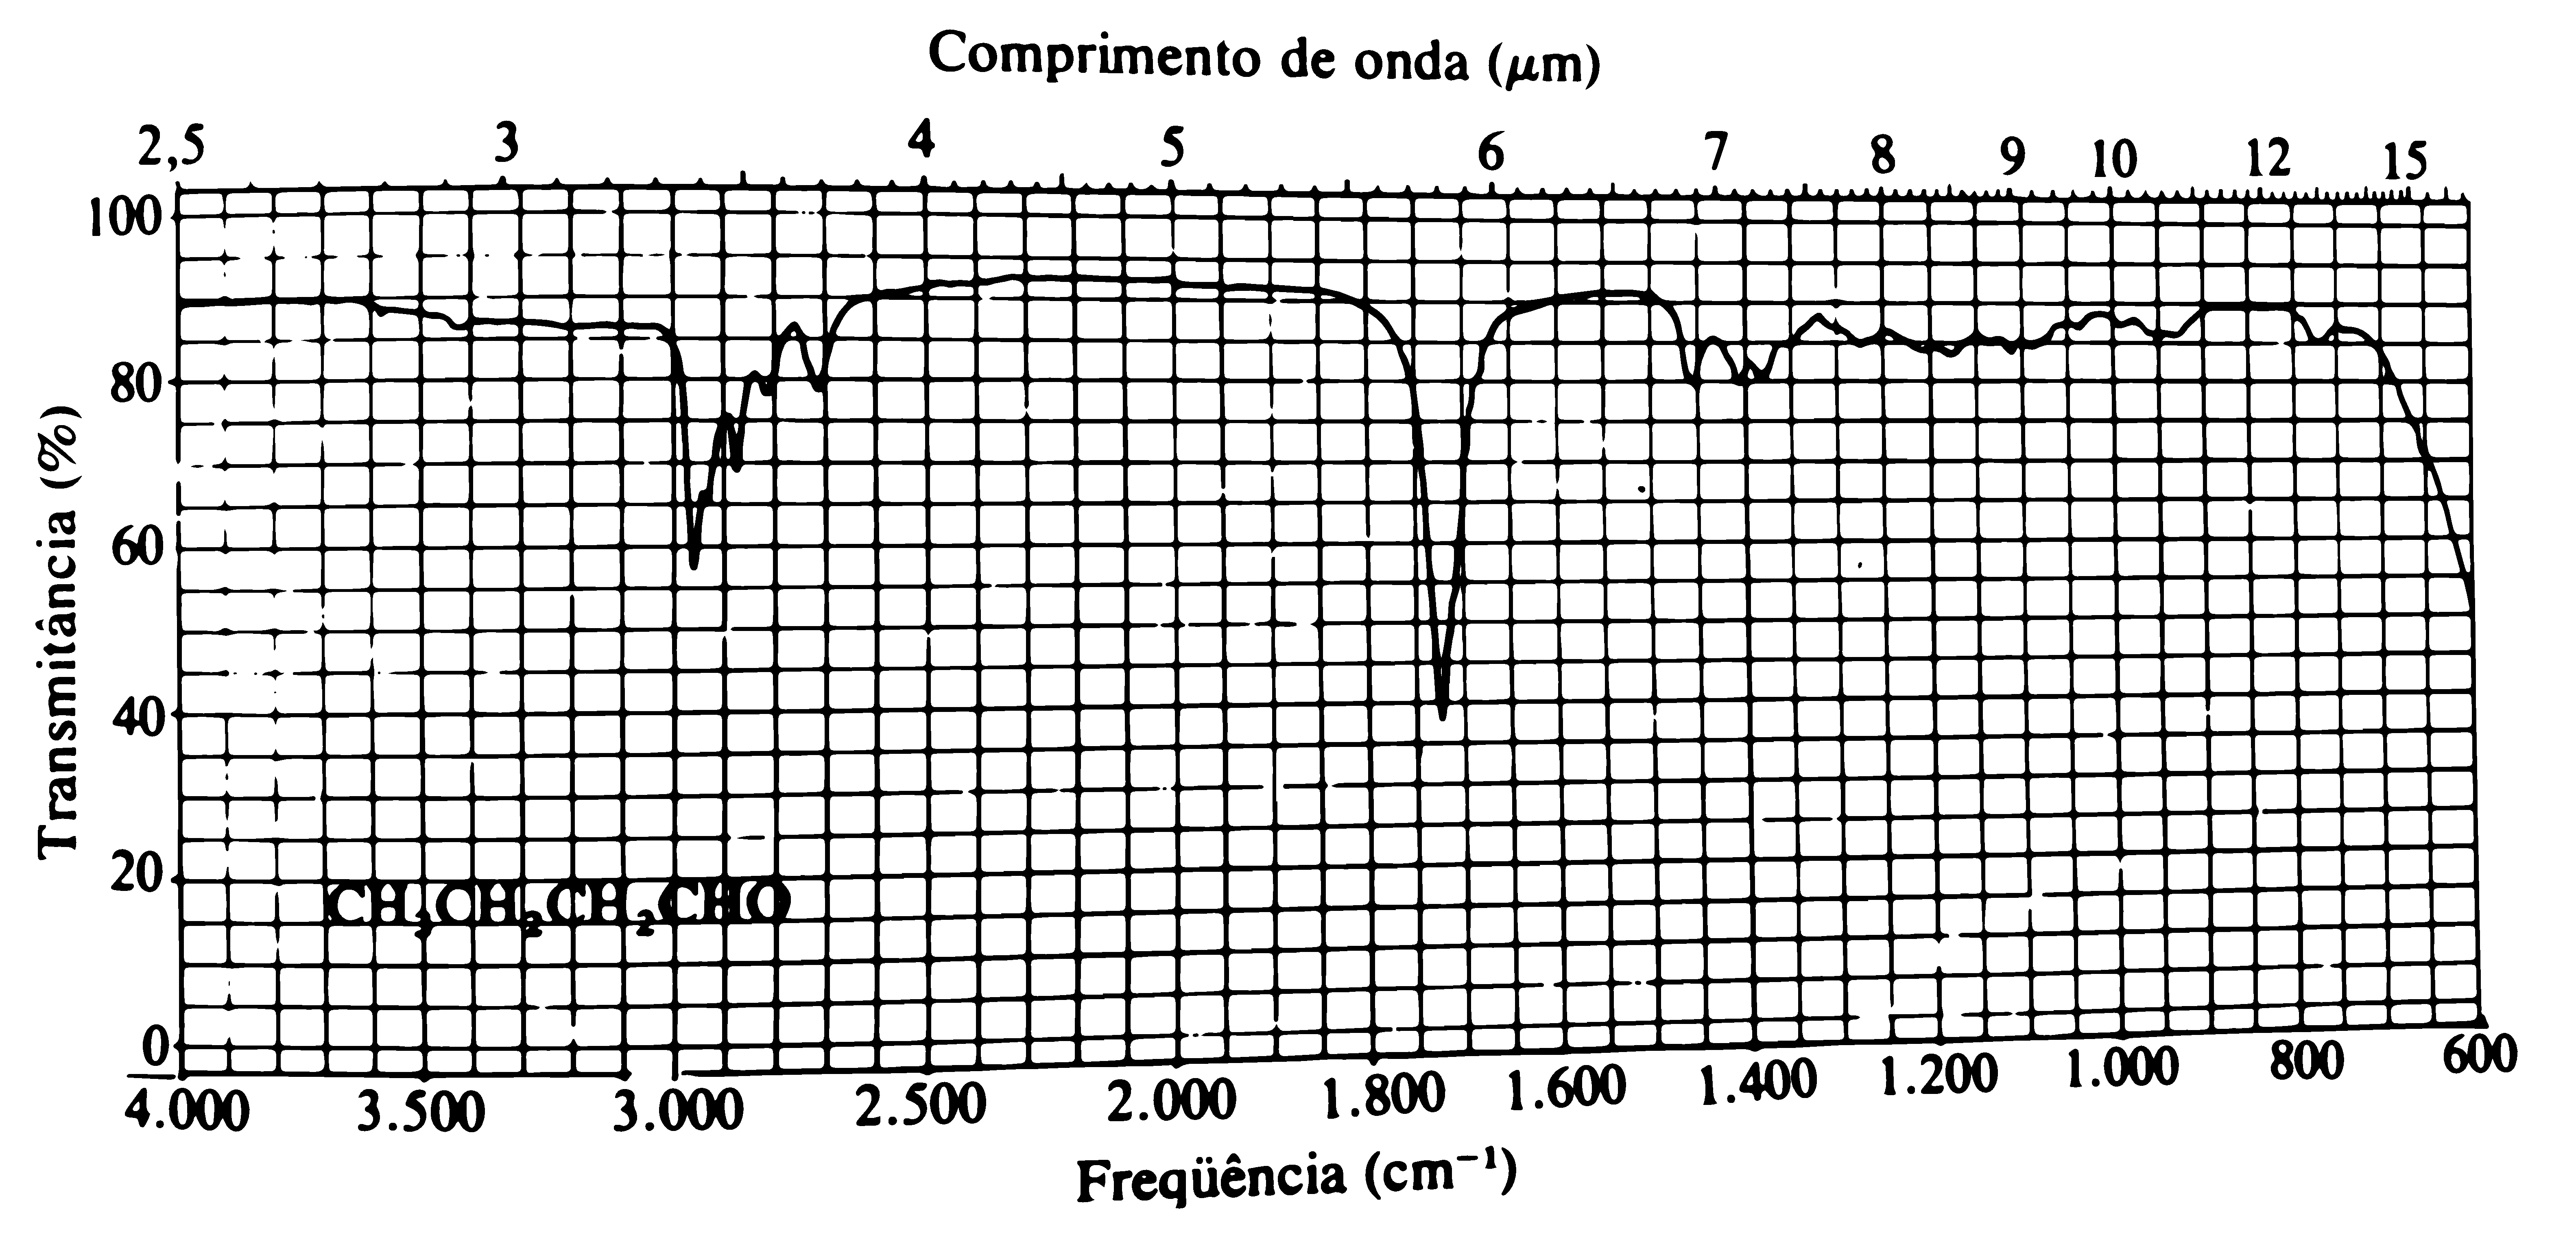
\includegraphics[width=0.9\textwidth,angle=0]{content/images/Figura_9_9.pdf}
    \caption{Espectro do butanal no infravermelho (filme líquido).}
    \label{figura_9_9}
\end{figure}

\begin{figure}[h]
    \centering
    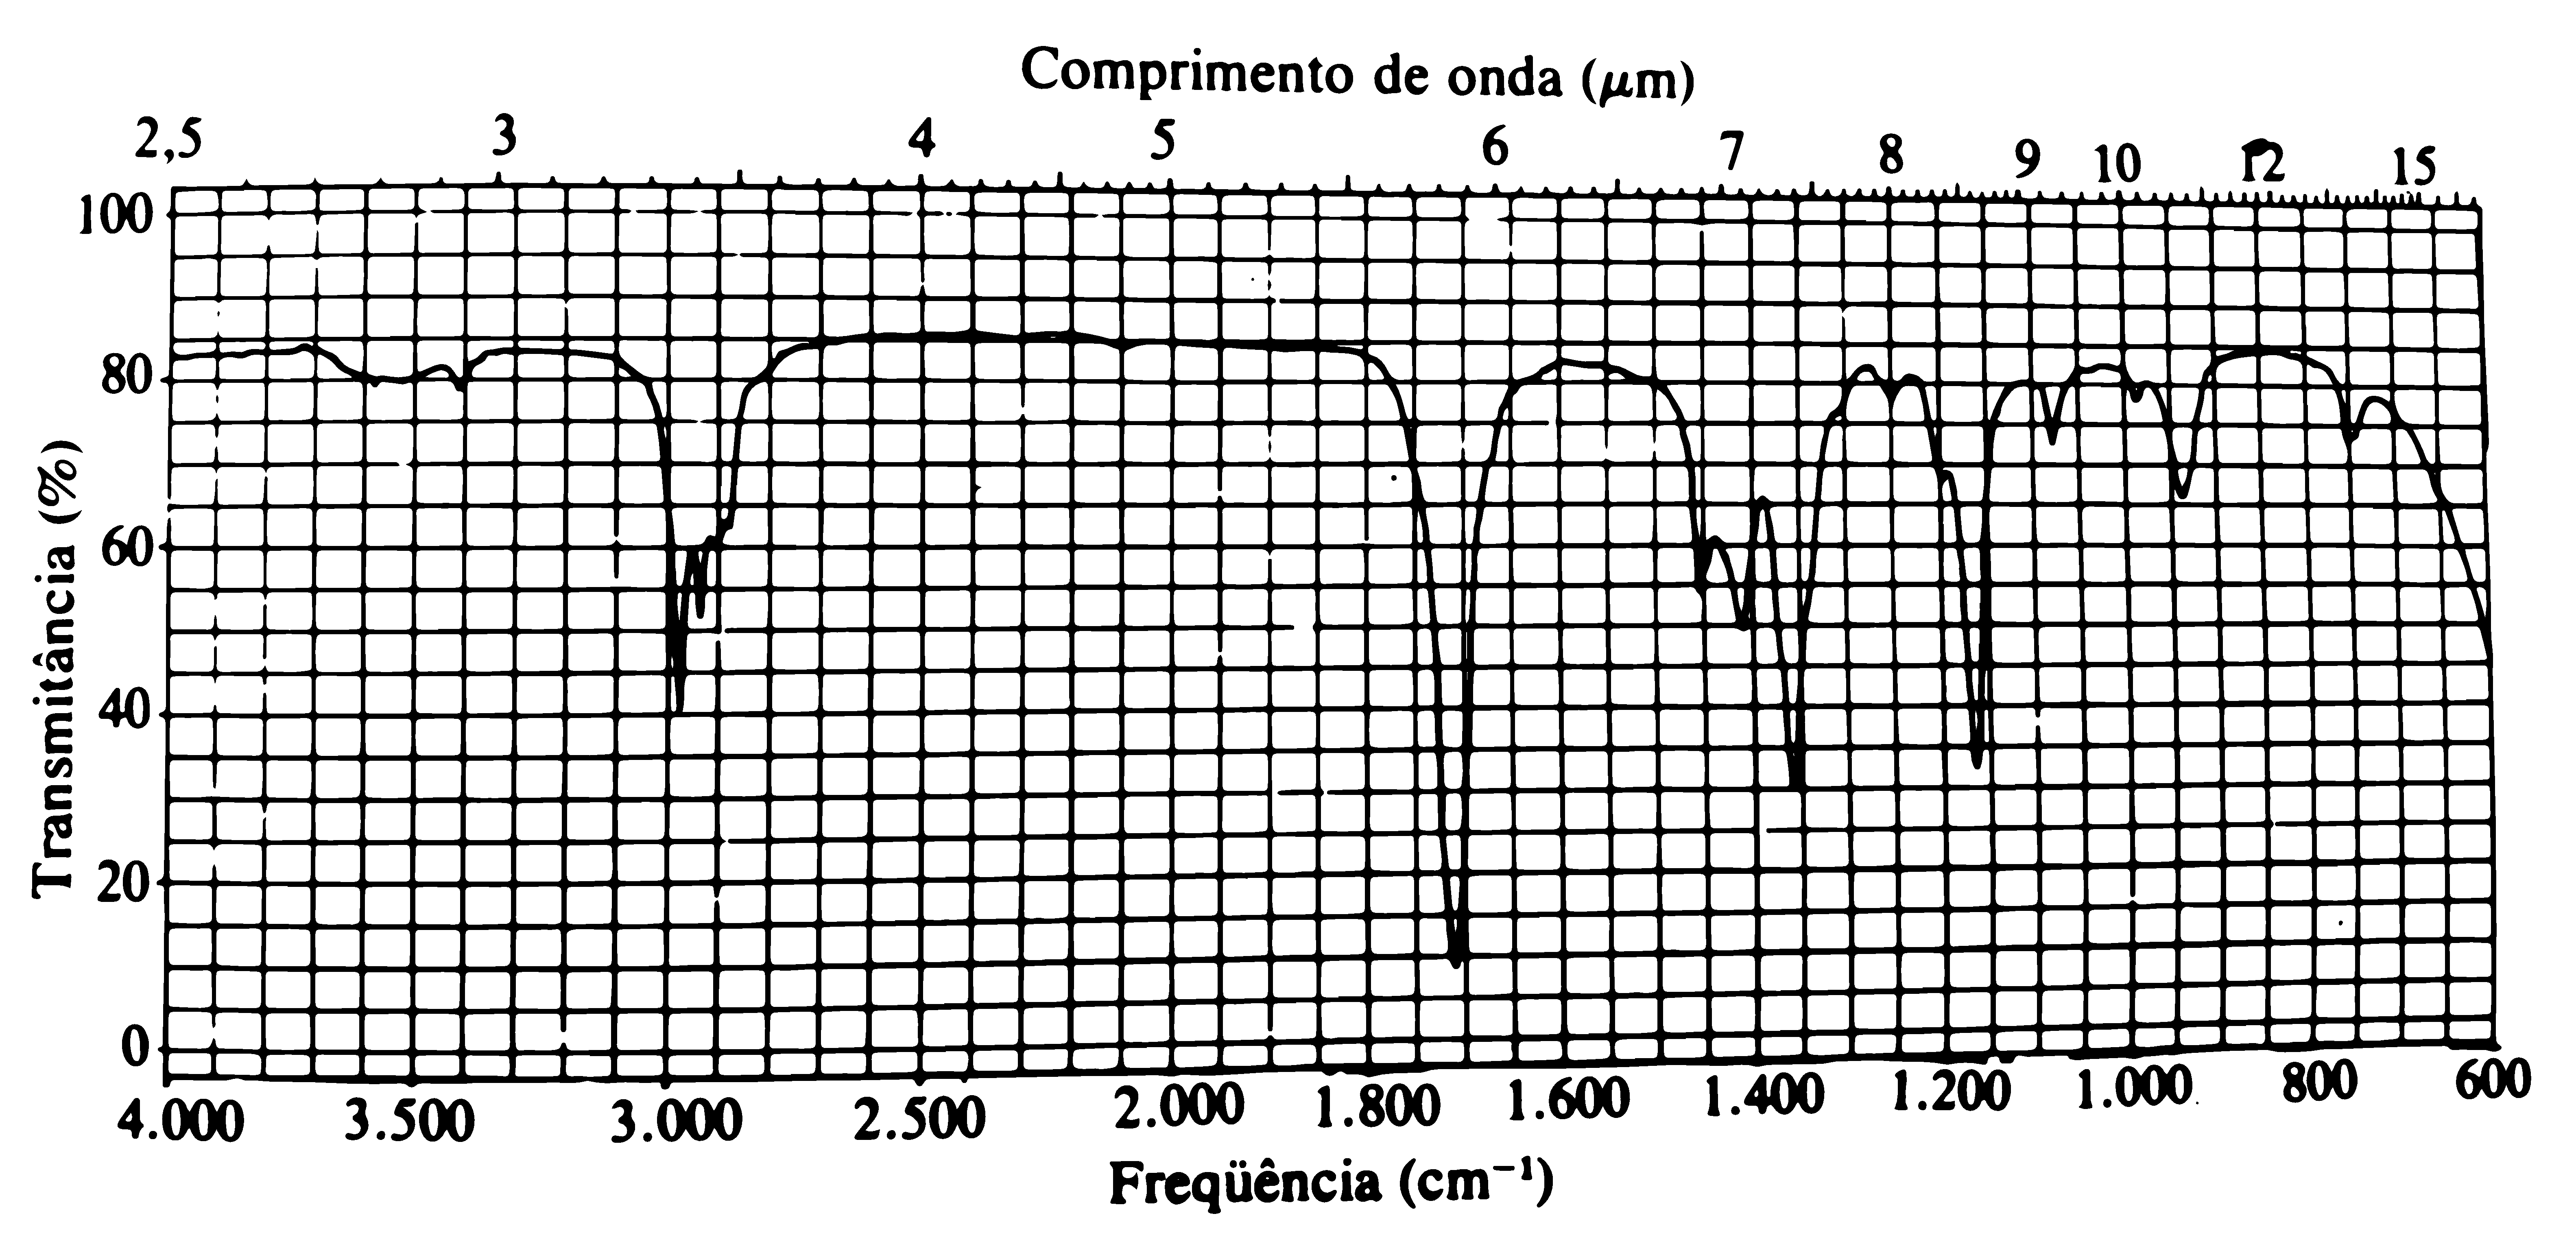
\includegraphics[width=0.9\textwidth,angle=0]{content/images/Figura_9_10.pdf}
    \caption{Espectro no infravermelho (filme líquido) de uma impureza isolada de butanal comercial e identificada como butanona.}
    \label{figura_9_10}
\end{figure}

\begin{figure}[h]
    \centering
    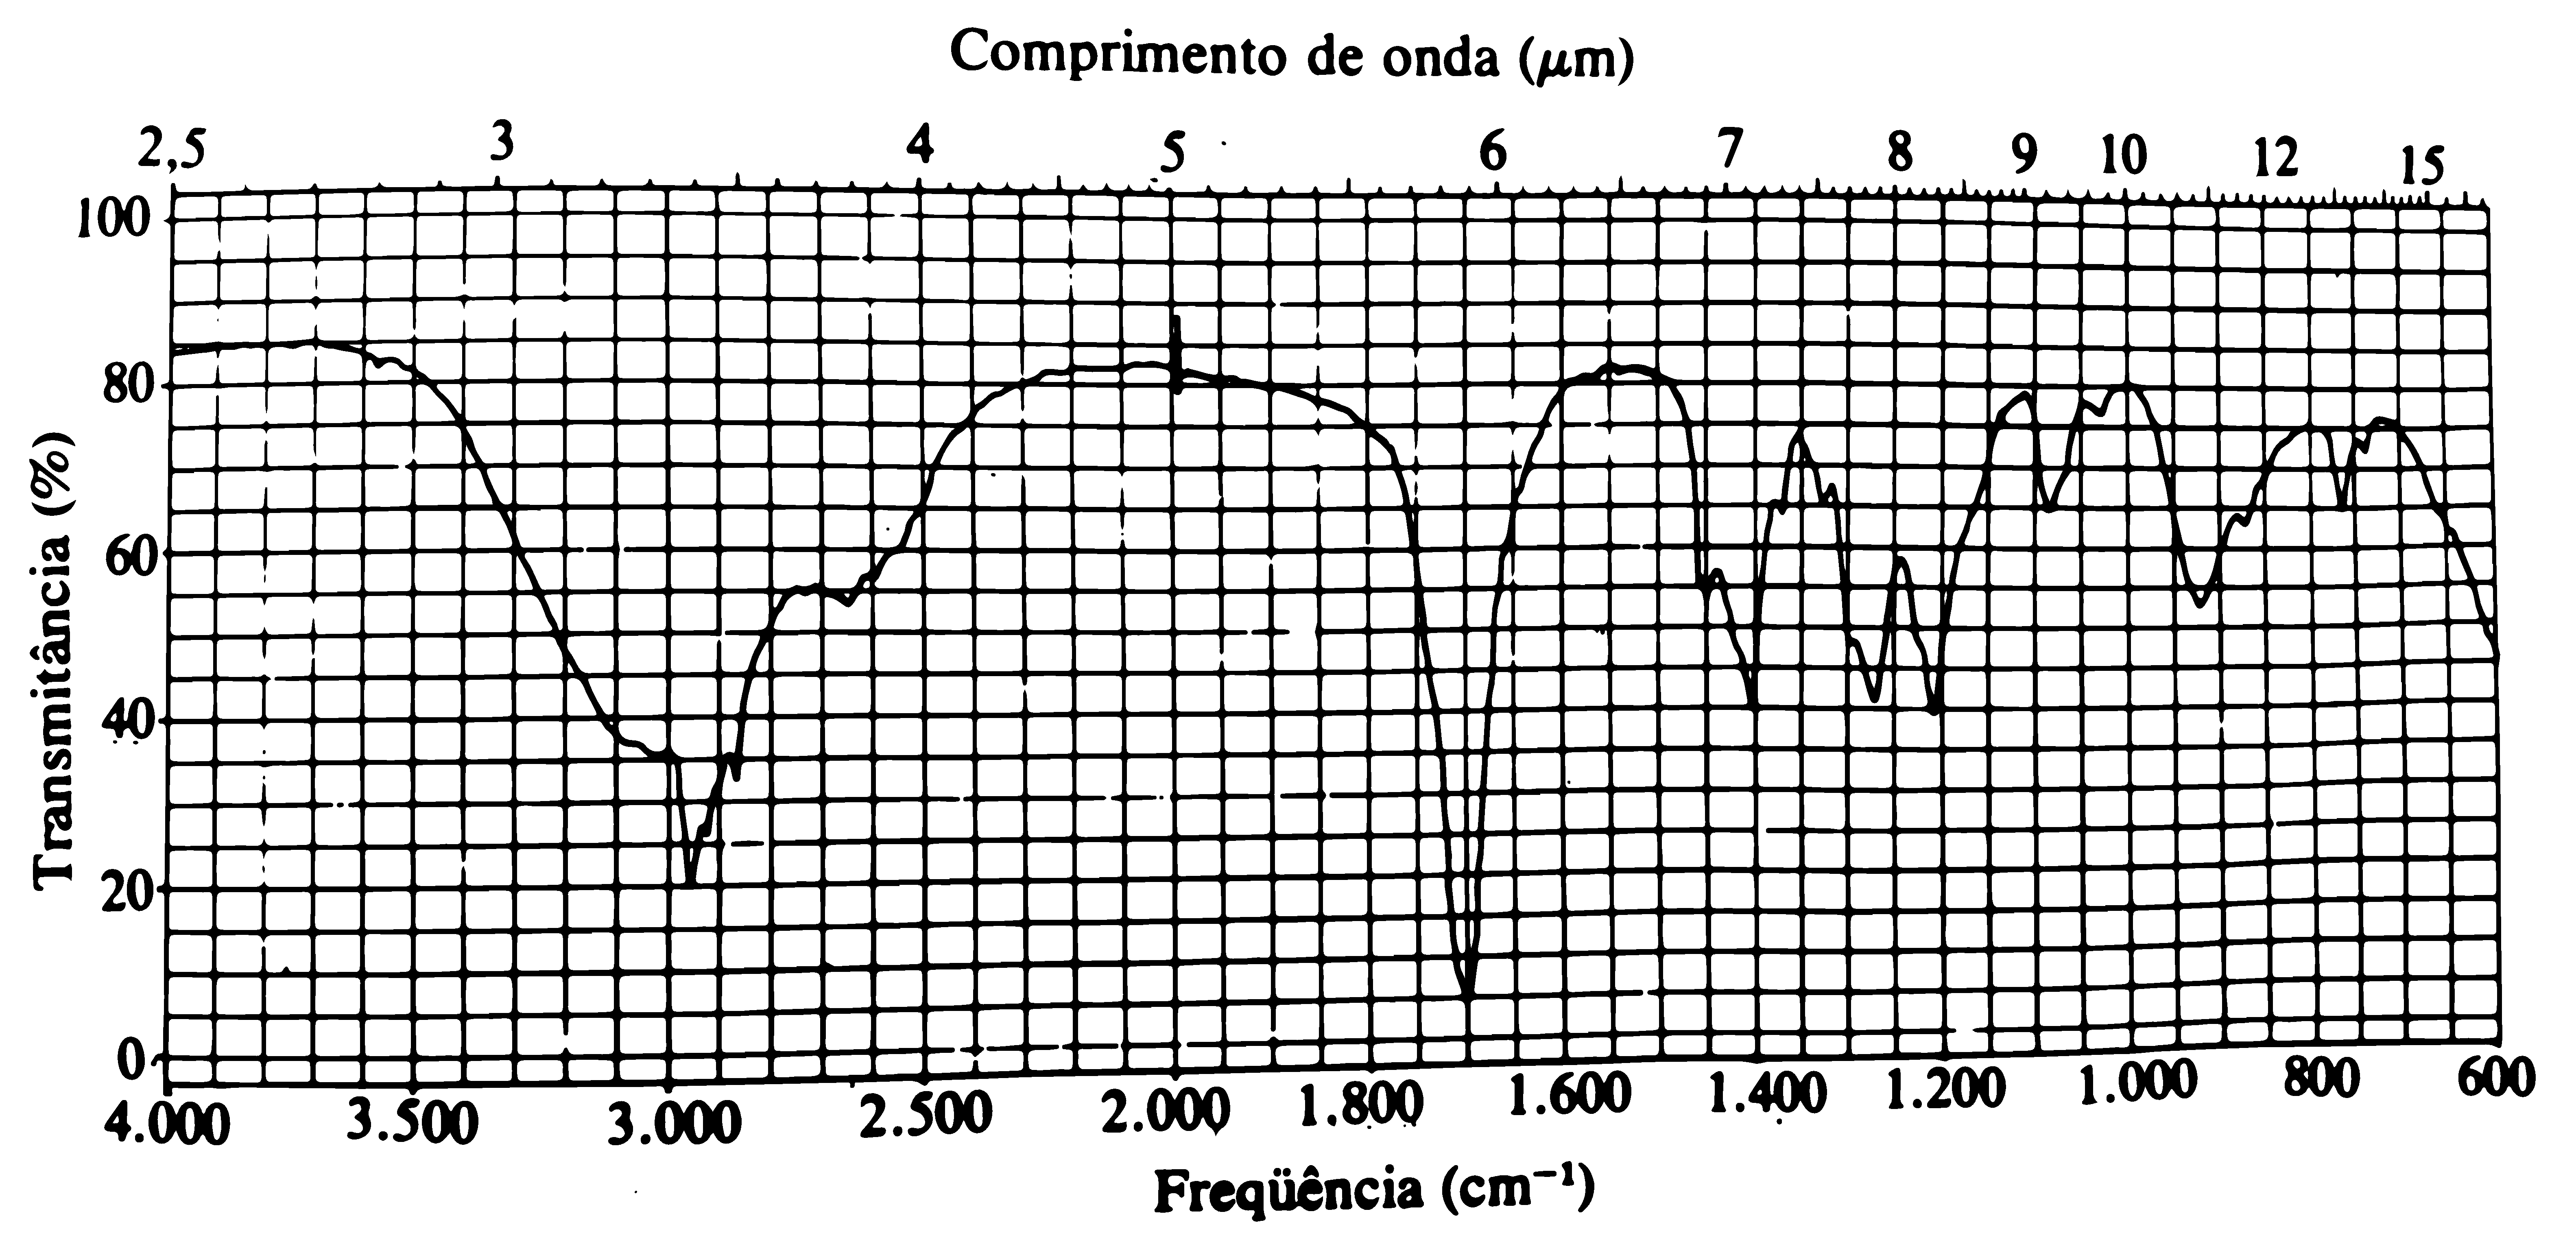
\includegraphics[width=0.9\textwidth,angle=0]{content/images/Figura_9_11.pdf}
    \caption{Espectro no infravermelho (filme líquido) de um composto desconhecido identificado como ácido butírico.}
    \label{figura_9_11}
\end{figure}

Existem outros classes de compostos, ainda não discutidos, para os quais pode-se obter informações e estruturais importantes a partir de seus espectros no infravermelho. Os fatos pertinentes serão apresentados quando estudarmos tais compostos. Veja o quadro no Apêndice para um sumário.

\end{document}
